% Summary results, v2 (final). Every number is read from FINAL_v2/v2_gridsearch/REPORT.md (run 2026-10-16 14:32, 31 datasets x 11 models)
% and the generated tables under paper/v2/tables/.  Compile from FINAL_v2/paper/ (tables resolve through \input@path) or as paper/v2/main.tex.
\documentclass[11pt]{article}
\usepackage[margin=1in]{geometry}
\usepackage{booktabs,graphicx,longtable,tabularx,array,caption,subcaption,amsmath,hyperref,enumitem,xcolor,pdflscape}
\usepackage{pdflscape}
\usepackage[T1]{fontenc}
\usepackage{lmodern}
\captionsetup{font=small,labelfont=bf}
\setlist{nosep,leftmargin=*}
\newcolumntype{L}{>{\raggedright\arraybackslash}X}
\graphicspath{{figures/}{v2/figures/}}
\makeatletter\def\input@path{{./}{v2/}}\makeatother
\emergencystretch=1.5em
\newcommand{\notable}[1]{\par\noindent\begingroup\small\textbf{Notable.} #1\endgroup\par\medskip}
\newcommand{\inoneline}[1]{\par\noindent\begingroup\small\textit{In one line: #1}\endgroup\par\medskip}
\hypersetup{colorlinks=true,linkcolor=blue!60!black,citecolor=blue!60!black,urlcolor=blue!60!black}

\title{Summary Results, v2}
\author{}
\date{2026}

\begin{document}
\maketitle

\section{Setup}
\label{sec:setup}

\subsection{Suite and pools}
\begin{itemize}
\item 31 datasets: 11 entity matching (EM), 6 schema matching (SM), 11 table question answering and understanding (TQA), 3 financial documents (FIN). Each adapter reads the official test or dev split and emits items with a question, a context (table, document, or record pair), a gold answer with aliases, a list gold where the answer is a set, an answer type (numeric / boolean / text / free-form) and the dataset's native metric.
\item Pools: 150 items per dataset by seeded stratified sampling (strata: question type, sub-task, database, product category, match label); 100 flagged for answering (OfficeQA Pro V2: all 90; Alaska schema: 93). The remaining 50 are a seeded reserve and are not used by any step. Total answered items: 3,083 per model.
\item Entity-matching pools are 50/50 match / non-match (Papadakis--Christen keeps its real 1.8\,\% match ratio). Schema matching is framed as one question per source column with a candidate list that always contains the gold. BIRD is graded on the executed result of the gold SQL, not on SQL text.
\item Official census: every dataset's official population is counted by the same strata, so that pool numbers can be re-weighted to the official split (Section~\ref{sec:setup:official}).
\end{itemize}

\subsection{Collecting answers}
\begin{itemize}
\item One prompt per item: context, question, and an answer-format line requesting \texttt{FINAL ANSWER: <answer>}.
\item Models (eleven): Claude Opus 5, Claude Sonnet 5, GPT-5.5, GPT-5.4-mini, Gemini 3.1 Pro, Gemini 3.8 Flash, Grok 4, DeepSeek-chat, DeepSeek-R1, gpt-oss-120b (Together), Llama 3.3 70B (Together). Gemini 3.1 Pro was collected over three weeks under Google's daily quota (a scheduled GitHub Actions workflow plus a final local run) and entered the study once it passed the 90\,\% coverage rule.
\item Decoding: temperature 0 where the API accepts it (Gemini, Grok, DeepSeek, Llama, gpt-oss). Claude 5 reports the parameter deprecated and GPT-5.5 rejects any non-default value; those ran at provider defaults. Every cached row records which applied.
\item Output budget 700 tokens. A reply cut off for length with no final-answer line is re-asked at 2,500 tokens, then 8,000, then 16,000 (and 32,000 for the two Claude Sonnet 5 replies still unfinished at 16,000). The trigger is mechanical (finish reason plus absence of the final line), never correctness. Originals are archived with a reason; replacement rows carry \texttt{attempt} = 2 to 5. The budget is counted in each provider's own tokens and, for the reasoning models, includes their chain of thought, so it is a termination test rather than an equal text allowance. Replies still unfinished at the last stage are scored as given (effectively failures): 41 DeepSeek-R1 answers at 16,000 tokens, plus 123 DeepSeek-R1 answers whose 16,000-token re-ask is pending on provider balance and stand at their 8,000-token replies.
\item Every answer is cached with tokens, latency, cost, finish reason and decoding; re-runs skip cached items. Cost: USD 174 for the answers in the final cache (Claude Opus 5: USD 107 including its re-asks; Gemini 3.1 Pro: USD 12), USD 224 over the whole project including the archived truncated originals.
\end{itemize}

\subsection{Scoring an answer}
\begin{itemize}
\item Extraction: the \texttt{FINAL ANSWER:} line; else a boxed expression; else the last short line of the reply.
\item Normalisation: Unicode NFKC, lower-case, canonical numbers (``1,577.00'' $\to$ ``1577'', ``(12.6)'' $\to$ ``$-$12.6''), currency symbols and punctuation removed, articles dropped, whitespace collapsed.
\item Units and scale: every number is parsed with sign, percent marker (\%, ``percent'', ``pp'') and scale word (thousand / million / billion / trillion and abbreviations). A parsed number exposes its equivalent readings (raw, scaled, $\div 100$ if marked percent, $\times 100$ if an unmarked fraction); the relative error between prediction and gold is the minimum over all pairs of readings. Real-unit conversions (km $\leftrightarrow$ miles) are not attempted.
\item Aliases: each item carries the primary gold plus acceptable alternatives supplied by the adapter (e.g.\ \emph{yes} $\equiv$ \emph{match} $\equiv$ 1; several legitimate target columns in schema matching; comma- and pipe-joined forms of list golds). Every component is computed against each alias and the best-scoring alias is kept. Booleans are canonicalised before comparison.
\item Components per answer: token F1, numeric decay $e^{-2.5\cdot\text{rel.\ err}}$ (error clipped at 2; falls back to exact match for non-numeric golds), token precision, token recall; also exact match, numeric tolerance (1\,\%), ROUGE-L, and a hedge flag (several distinct numeric candidates, ``A or B'', or an enumeration of short candidates).
\item Native metric per dataset (baseline column): numeric tolerance for numeric golds, exact match for text and boolean golds, ROUGE-L for free-form (FeTaQA).
\item Composite under weighting $w$ on the simplex: $R_w = \sum_k w_k m_k$, $k \in \{$F1, decay, precision, recall$\}$. v1 is $w = (0.35, 0.35, 0.15, 0.15)$.
\item Dataset score of a model: mean $R_w$ over the items that every model answered. A model is in the study only if it covered $\ge 90\,\%$ of the suite; a dataset is used only with $\ge 20$ answered items.
\end{itemize}

\subsection{Evaluating a weighting}
\begin{enumerate}
\item \textbf{Agreement $J(w)$.} Rank the eleven models inside each dataset under $w$; pool the 31 rankings by Borda; $J$ is the mean Kendall $\tau_b$ between each dataset's ranking and the pooled one. $J$ measures consistency between datasets, not correctness. Computed for all 1,771 weightings of the step-0.05 simplex lattice (v1, the four corners and the uniform mix are lattice points), and also under Kemeny, Copeland and Bradley--Terry pooling.
\item \textbf{Correctness $\rho(w)$.} 31,380 synthetic answers of known utility generated from the golds of the answered items by typed operators (identity, alias, unit variant, typo, rounding, magnitude error, sign flip, wrong value, partial list, superset, hedge, verbose, no answer, \dots). Reported: Spearman $\rho$ between $R_w$ and utility, AUC correct vs wrong, mean score of wrong answers, hedge gap; the $(J,\rho)$ Pareto front and its knee.
\item \textbf{Honest selection.} Nested item bootstrap ($B=1{,}000$): choose the best $w$ on in-bag items, score it out of bag. Reported: the optimism gap, the paired out-of-bag difference to v1 with a 95\,\% interval, and the plateau (weightings not significantly below the best, paired bootstrap $p>.05$) plus a practical plateau (within 0.02 of the best).
\item \textbf{Transfer.} Leave-one-dataset-out and leave-one-family-out: re-fit $w$ on the rest, measure $\tau$ of the held-out dataset's ranking to the pooled rest; per-family optima; sensitivity to one lattice step (0.05).
\item \textbf{Designs.} Uniform-lattice, Dirichlet-snapped and Latin-hypercube samples of 100 weightings, 20 seeds each, compared with the exhaustive optimum (regret, rank of the found best, centred $L_2$ discrepancy, minimum pairwise $L_1$).
\end{enumerate}

\subsection{From scores to a leaderboard}
\label{sec:setup:official}
\begin{itemize}
\item Rules reported: exact match only, v1, the five best by $J$, the best by $\rho$, the $(J,\rho)$ Pareto knee.
\item Pooling: Bradley--Terry strengths from item-level pairwise wins (MLE, ridge 0.01, standard errors from the observed information) as the headline; Borda, mean-$z$, Kemeny (with cost), Copeland, reciprocal-rank fusion and family-balanced $z$ as checks.
\item Uncertainty: 1,000 item bootstraps of the Borda and Bradley--Terry rankings (rank intervals, probability of first place), saved in full.
\item Significance: Friedman with the Iman--Davenport correction across datasets, Nemenyi critical difference, Holm-corrected pairwise Wilcoxon; paired permutation and Wilcoxon per dataset and model pair (Holm within dataset); Kendall's $W$ among datasets; majority-class baselines for boolean sets.
\item Official-split estimates: the same answers re-weighted by official stratum share / sample share (post-stratification) with a weighted item bootstrap; positive-class precision, recall and F1 at the official match ratio for the matching sets.
\item Diagnostics: pairwise $\tau$ between dataset rankings; floor, ceiling and self-stability flags per dataset.
\item Reporting: one script regenerates the report from the cached answers in minutes, so text and numbers cannot disagree.
\end{itemize}

\section{Results}
\label{sec:results}

All numbers are from the run of 2026-10-16 (31 datasets $\times$ 11 models, 3,083 answered items per model). Table~\ref{tab:summary} gives the audit in one place; the subsections that follow give one figure or table per row.

\begin{table}[htbp]
\centering\small
\caption{Audit summary. $J$ = agreement objective (mean Kendall $\tau_b$ of each dataset's model ranking to the Borda pool); $\rho$ = Spearman correlation of the composite with known utility on 31,380 synthetic anchors.}
\label{tab:summary}
\begin{tabularx}{\textwidth}{>{\bfseries}p{0.30\textwidth} L}
\toprule
Exhaustive grid & 1,771 weightings (step 0.05); best F1 .35 / decay .60 / precision .05 / recall 0, $J=0.414$; v1 $J=0.392$ (rank 1,602 of 1,771) \\
$J$ over the lattice & range 0.376--0.414; median 0.401, 90th percentile 0.407, 99th percentile 0.412: a flat landscape \\
Plateau (paired bootstrap $p>.05$ vs best) & 1,749 of 1,771 (v1 inside, $p=0.63$); practical plateau within 0.02: 1,731 \\
Nested selection ($B=1{,}000$) & in-bag $J$ of the selected weighting 0.370, out-of-bag 0.323 (optimism gap 0.047); v1 out-of-bag 0.330 \\
Selected vs v1, out of bag & $-0.007$, 95\,\% CI $[-0.033,\,+0.011]$, $p=0.72$; 624 distinct weightings selected across resamples \\
Sampled designs (100 points, 20 seeds) & Dirichlet / LHS / uniform all reach $0.412$--$0.413\pm0.001$, regret $\le 0.004$: sampling would have sufficed \\
Objective under other pooling rules & Kemeny, Copeland and Bradley--Terry each pick a different ``best''; v1's rank swings from 615 (Bradley--Terry) to 1,602 (Borda): rank is noise \\
Transfer (leave-one-dataset-out) & held-out $\tau$: re-fitted weights $+0.33$, full best $+0.35$, v1 $+0.32$ \\
Leave-one-family-out & v1 within 0.05 of the held-out-fitted weights in every family (EM $+0.32$ vs $+0.32$, SM $+0.28$ vs $+0.33$, TQA $+0.33$ vs $+0.33$, FIN $+0.44$ vs $+0.45$) \\
Anchors (31,380 synthetic answers) & v1 $\rho=0.878$, best-$\rho$ weighting 0.883, best-$J$ weighting 0.876, exact match 0.828; AUC correct-vs-wrong 0.994 for every rule \\
$J$ vs $\rho$ across the lattice & $-0.23$ (was $-0.34$ at ten models and $+0.38$ on the 2,500-token cache): unstable because $J$ is flat; Pareto front of 17, knee = best $J$ \\
Sensitivity & one 0.05 step moves $J$ by at most 0.012 around v1 and 0.017 around the best \\
Leaderboard & Friedman $p<0.001$ under every rule; Kendall's $W$ among datasets 0.26--0.27 \\
Significant pairs (Holm, v1) & 15 of 55: nine models $>$ Llama 3.3 70B; Opus, GPT-5.5, Gemini 3.1 Pro, Gemini 3.8 Flash, DeepSeek-R1 and Grok 4 $>$ gpt-oss-120b \\
First place & Bradley--Terry: Gemini 3.8 Flash under v1 and every calibrated rule ($P(\text{first})$ 0.91--0.95), Claude Opus 5 under exact match (0.79); Borda: GPT-5.5 under v1 and the calibrated rules, Opus under exact match \\
Gemini 3.1 Pro & enters fifth by Bradley--Terry under v1 (fourth under exact match), below Flash, Opus, GPT-5.5 and Sonnet \\
Official-split comparability & accuracy moves by $\le 0.09$ after post-stratification (OpenSanctions); positive-class F1 on the balanced pools overstates official-ratio F1 by up to 0.19 (Amazon--Google) \\
Datasets at ceiling & Valentine, WDC LSPC, WDC Products (means 0.98): flagged; still inside the objective \\
Cost & USD 174 for the final cache (Opus 107); USD 224 over the project including archived truncated originals \\
\bottomrule
\end{tabularx}
\end{table}

\subsection{The objective is flat}
\inoneline{Every weighting of the four ingredients gives nearly the same agreement; v1's low rank is a rank inside noise.}
Figure~\ref{fig:landscape} shows $J$ for all 1,771 weightings. The whole lattice spans 0.376--0.414. The best weighting (F1 0.35, decay 0.60, precision 0.05) reaches 0.414 and v1 reaches 0.392; 1,601 weightings are nominally better than v1, but the entire spread is smaller than the bootstrap noise of a single weighting (about 0.027). No single weight has a slope worth acting on (Figure~\ref{fig:marginals}); the four ingredients correlate at 0.91--0.98 with one another and in 82\,\% of answers all four equal exact match, which is the mechanical reason.

\begin{figure}[htbp]
\centering
\begin{subfigure}{0.48\textwidth}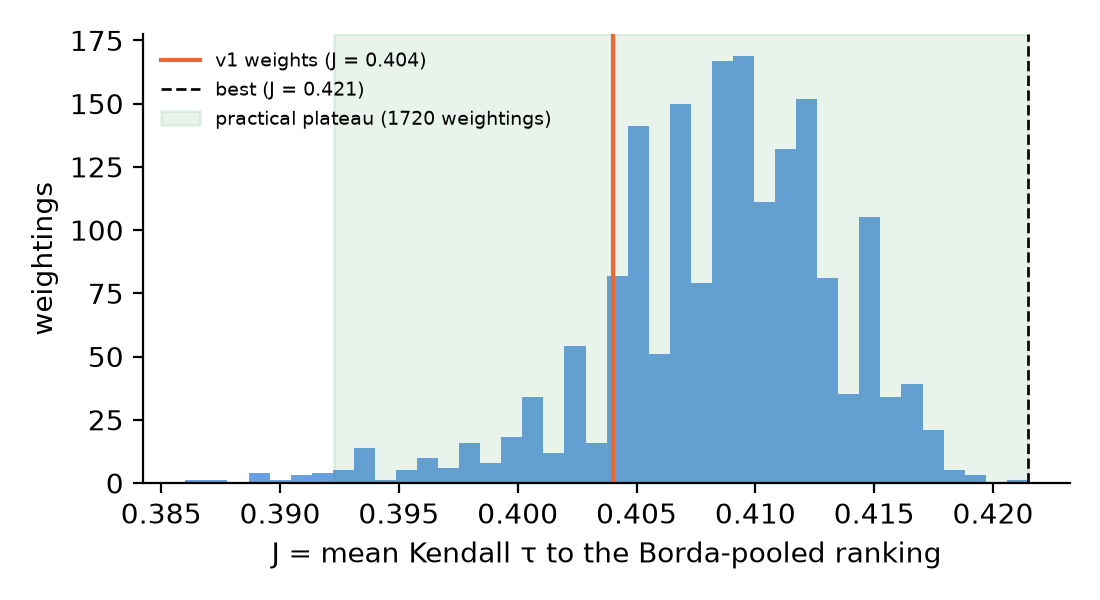
\includegraphics[width=\linewidth]{fig_j_histogram.png}\caption{Distribution of $J$ over the lattice with v1, the best and the plateau band.}\end{subfigure}\hfill
\begin{subfigure}{0.48\textwidth}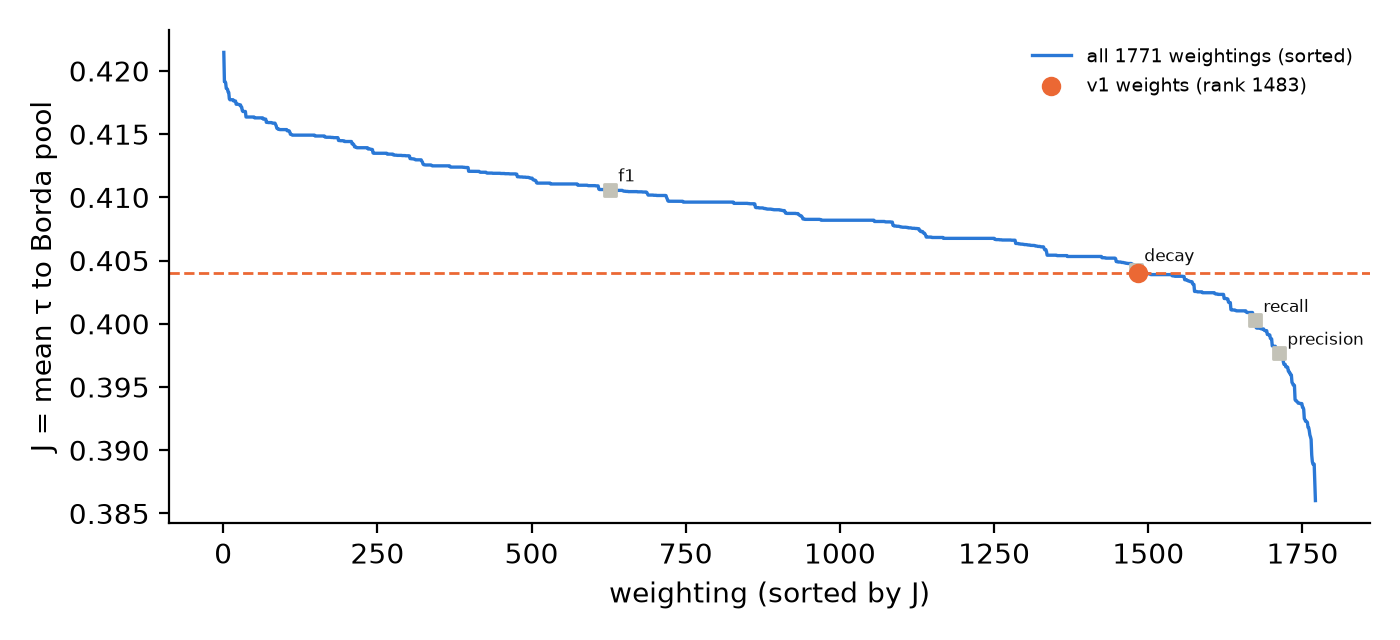
\includegraphics[width=\linewidth]{fig_landscape.png}\caption{Sorted $J$ with v1 and the four single-ingredient corners.}\end{subfigure}
\caption{The agreement landscape over all 1,771 step-0.05 weightings.}
\label{fig:landscape}
\end{figure}
\notable{(a) The histogram is narrow: 1,771 weightings fit between 0.376 and 0.414, and v1 (0.392) sits in the main body, not in a tail. (b) The sorted curve is flat for 1,700 weightings and only drops at the single-ingredient corners; v1's rank of 1,602 is a position on a plateau, which is why the report never quotes rank as a result.}

\begin{figure}[htbp]
\centering
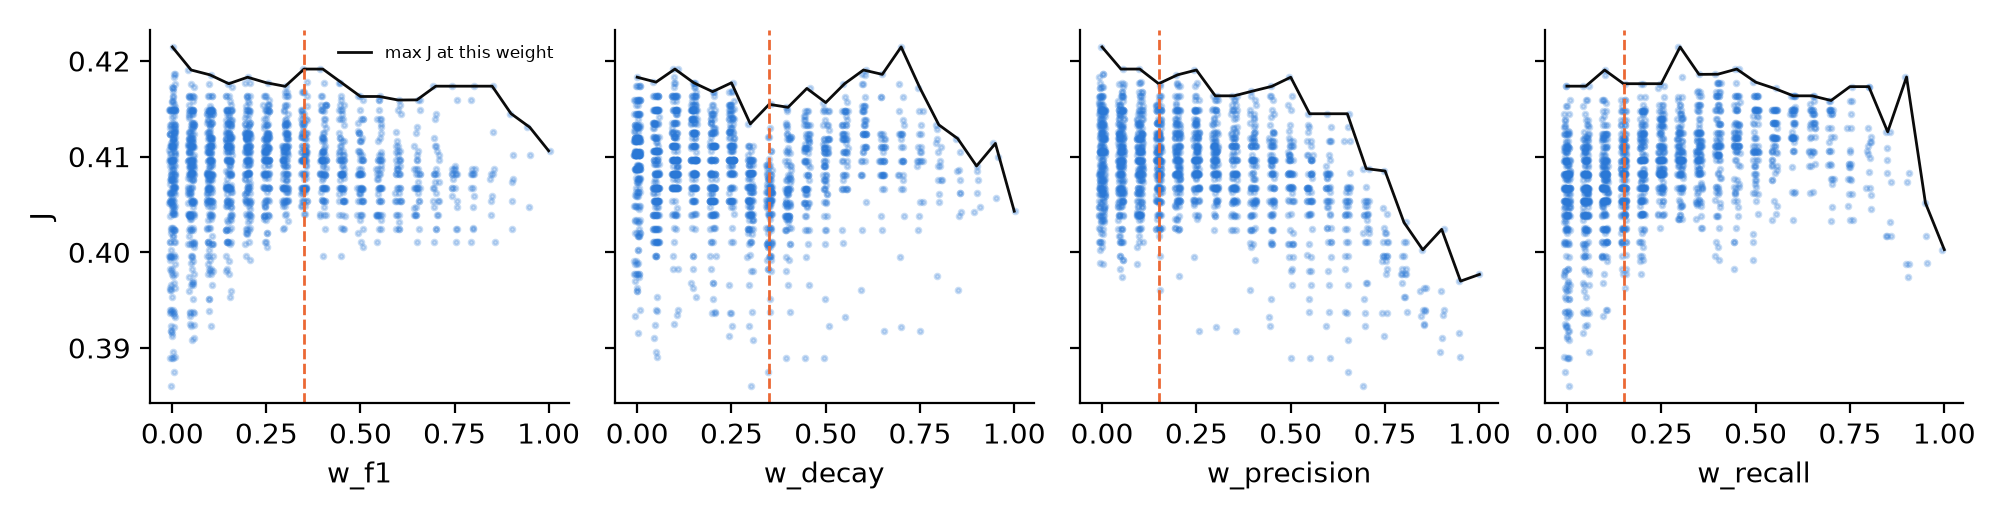
\includegraphics[width=0.95\textwidth]{fig_marginals.png}
\caption{$J$ against each of the four weights. Corners: F1 only 0.409, decay only 0.394, precision only 0.386, recall only 0.389; uniform 0.401.}
\label{fig:marginals}
\end{figure}
\notable{No panel has a slope worth acting on: the mean line moves by at most 0.018 across the full range of any weight (precision, falling as it approaches 1). The vertical scatter at every weight level, caused by the other three weights, is wider than any slope, so no ingredient can be tuned in isolation.}

\subsection{The best weighting does not survive honest selection}
\inoneline{Chosen honestly, the best weighting is no better than v1; 624 different weightings win depending on which items are drawn.}
Figure~\ref{fig:nested} reports the nested item bootstrap. The weighting chosen on in-bag items scores 0.370 in bag but 0.323 out of bag (optimism gap 0.047), below v1's out-of-bag 0.330. The paired out-of-bag difference to v1 is $-0.007$ with a 95\,\% interval of $[-0.033, +0.011]$ ($p=0.72$); the selected weighting is ahead of v1 in 28\,\% of resamples, and 624 distinct weightings were selected across the 1,000 resamples. The plateau of weightings not significantly below the best contains 1,749 of 1,771 points and v1 is inside it ($p=0.63$).

\begin{figure}[htbp]
\centering
\begin{subfigure}{0.48\textwidth}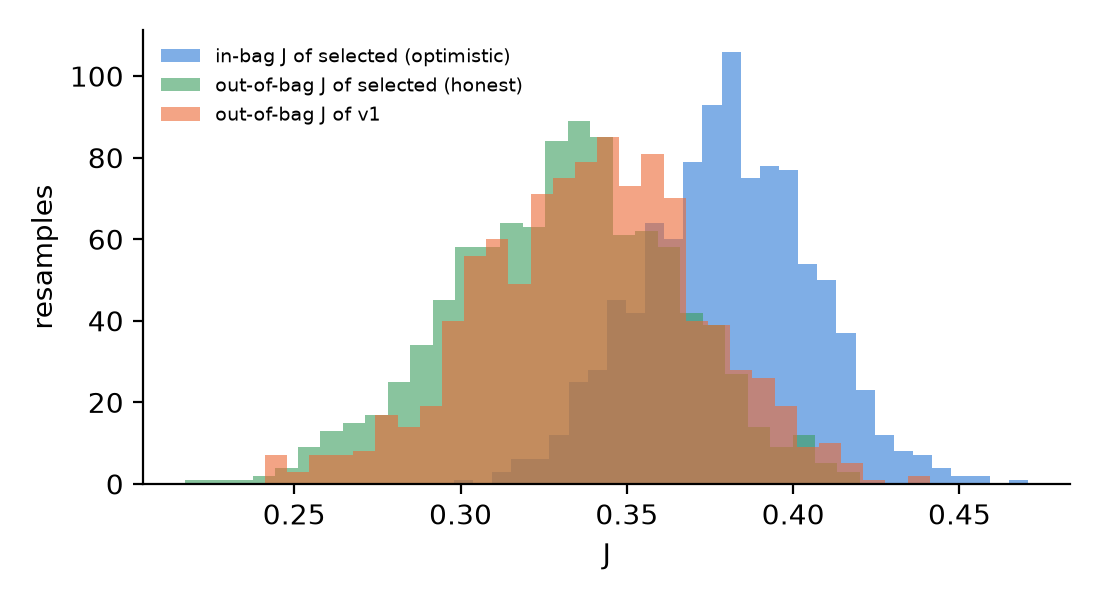
\includegraphics[width=\linewidth]{fig_nested.png}\caption{In-bag vs out-of-bag $J$ of the selected weighting against v1.}\end{subfigure}\hfill
\begin{subfigure}{0.48\textwidth}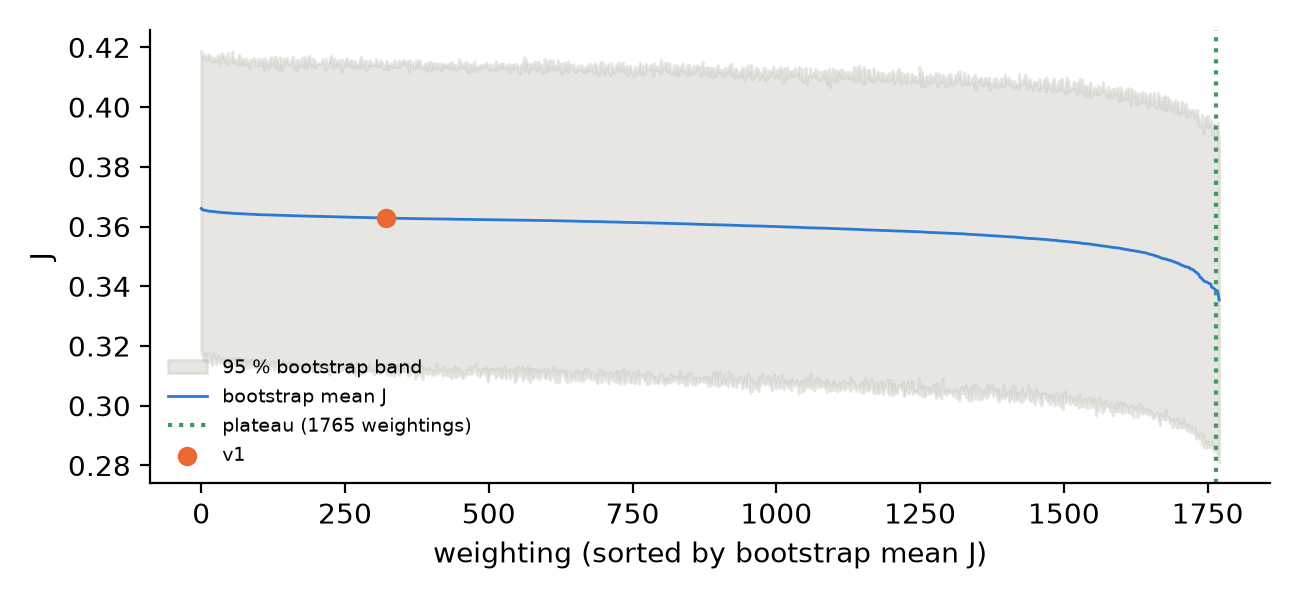
\includegraphics[width=\linewidth]{fig_plateau.png}\caption{Bootstrap band over sorted weightings; the plateau boundary.}\end{subfigure}
\caption{Honest selection: the optimism gap and the plateau.}
\label{fig:nested}
\end{figure}
\notable{(a) The in-bag winner looks 0.047 better than it is; out of bag it scores 0.323 against v1's 0.330, and the paired difference of $-0.007$ has a 95\,\% interval through zero. (b) 1,749 of 1,771 weightings are inside the plateau and v1 is one of them ($p = 0.63$); the only points outside are decay-dominated corners with no F1 or recall.}

\begin{table}[htbp]
\centering\scriptsize
\caption{Sampled designs at a budget of 100 weightings, 20 seeds each, against the exhaustive optimum.}
\label{tab:designs_short}
\setlength{\tabcolsep}{3pt}
\begin{tabular}{p{0.451\linewidth}p{0.189\linewidth}rp{0.160\linewidth}r}
\toprule
design & best J (mean) & sd & regret mean & regret max \\
\midrule
dirichlet\_\allowbreak{}lattice & 0.4123 & 0.0012 & 0.0020 & 0.0041 \\
lhs\_\allowbreak{}simplex & 0.4126 & 0.0012 & 0.0017 & 0.0038 \\
uniform\_\allowbreak{}lattice & 0.4125 & 0.0012 & 0.0018 & 0.0041 \\
\bottomrule
\end{tabular}
\end{table}

\notable{All three 100-point designs reach 0.412--0.413 with a worst-seed regret of 0.004 against the exhaustive 0.414. With four weights the exhaustive grid costs nothing, so the table matters only as evidence that sampling would have sufficed in the larger sibling searches.}

\begin{figure}[htbp]
\centering
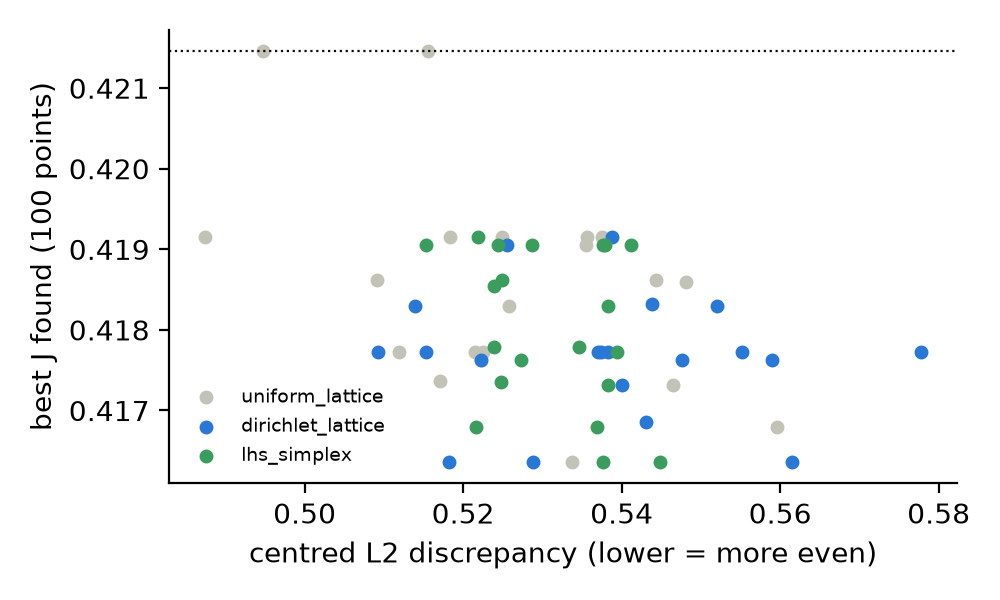
\includegraphics[width=0.8\textwidth]{fig_designs.png}
\caption{Any 100-point design finds the plateau; regret against the exhaustive optimum is at most 0.004.}
\label{fig:designs}
\end{figure}


\subsection{The optimum does not transfer, and neither does the rank}
\inoneline{Re-fitted weights predict a held-out dataset no better than v1, and families want different weights.}
Leave-one-dataset-out: weights re-fitted without the held-out dataset predict its ranking with mean $\tau=+0.33$, the full-data best with $+0.35$, v1 with $+0.32$ (Table~\ref{tab:lofo_short} gives the family-level version). Per-family optima pull in different directions (Figure~\ref{fig:family}): decay-only for schema matching, recall-heavy for table QA and finance, F1-and-decay for entity matching, yet none is far from the plateau. Changing only the pooling rule inside the objective moves v1's rank from 615 (Bradley--Terry) to 1,602 (Borda) and changes which weighting is ``best'', so rank inside a flat objective carries no information.

\begin{table}[htbp]
\centering\scriptsize
\caption{Leave-one-family-out: weights re-fitted without the family (F1 / decay / precision / recall) and the held-out family's $\tau$ to the pooled rest under those weights, the full-data best and v1.}
\label{tab:lofo_short}
\setlength{\tabcolsep}{3pt}
\begin{tabular}{lp{0.269\linewidth}p{0.194\linewidth}p{0.194\linewidth}p{0.194\linewidth}}
\toprule
family & LOFO weights & tau: LOFO weights & full best & v1 \\
\midrule
EM & 0.70 / 0.15 / 0.05 / 0.10 & 0.320 & 0.312 & 0.316 \\
SM & 0.05 / 0.25 / 0.00 / 0.70 & 0.329 & 0.304 & 0.280 \\
TQA & 0.05 / 0.00 / 0.60 / 0.35 & 0.335 & 0.367 & 0.330 \\
FIN & 0.05 / 0.75 / 0.05 / 0.15 & 0.449 & 0.489 & 0.440 \\
\bottomrule
\end{tabular}
\end{table}

\notable{Held-out $\tau$ under re-fitted weights is within 0.05 of v1 in every family (EM $+0.32$ vs $+0.32$, SM $+0.33$ vs $+0.28$, TQA $+0.33$ vs $+0.33$, FIN $+0.45$ vs $+0.44$). The re-fitted weights themselves swing from F1-heavy (EM) to recall-heavy (SM) to decay-heavy (FIN): there is no single weighting the families agree on.}

\begin{figure}[htbp]
\centering
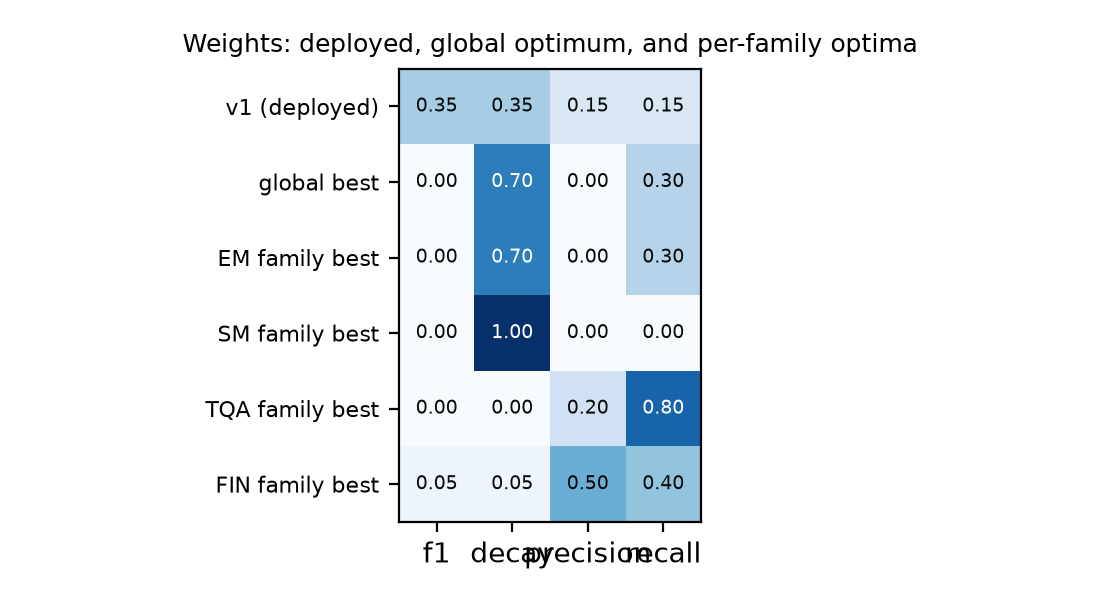
\includegraphics[width=0.85\textwidth]{fig_family_weights.png}
\caption{Deployed weights (v1), the global optimum and the per-family optima.}
\label{fig:family}
\end{figure}
\notable{Schema matching wants decay only, table QA and finance want recall-heavy mixes, entity matching wants F1 and decay; the global optimum is a compromise between them, and v1 is another. The suite-level flatness is partly these pulls cancelling, which is also why leave-one-family-out re-fits land far from the global best without doing better on the held-out family.}

\subsection{Agreement and correctness do not pull the same way}
\inoneline{Agreement among datasets and correctness on known answers are different criteria; v1 is near the correctness optimum.}
On 31,380 synthetic answers of known utility, v1 scores $\rho=0.878$; the best weighting by $\rho$ reaches 0.883 and the best by $J$ 0.876; exact match 0.828. Every rule separates correct from wrong answers with AUC 0.994. Across the lattice $J$ and $\rho$ correlate $-0.23$ on this cache, $-0.34$ at ten models and $+0.38$ on the earlier 2,500-token cache, which is what a flat $J$ predicts. With eleven models the Pareto knee coincides with the best-$J$ weighting (Table~\ref{tab:anchors_rules}, Figure~\ref{fig:pareto}).

\begin{landscape}
\begin{table}[htbp]
\centering\tiny
\caption{Anchor correctness for the labelled rules.}
\label{tab:anchors_rules}
\setlength{\tabcolsep}{3pt}
\resizebox{\linewidth}{!}{%
\begin{tabular}{lrrrrrrrrrrrr}
\toprule
label & rank & w\_\allowbreak{}f1 & w\_\allowbreak{}decay & w\_\allowbreak{}precision & w\_\allowbreak{}recall & J & tau\_\allowbreak{}native & rho & rho\_\allowbreak{}ds & auc & wrong\_\allowbreak{}mean & hedge\_\allowbreak{}gap \\
\midrule
only\_\allowbreak{}f1 & 96 & 1.000 & 0.000 & 0.000 & 0.000 & 0.409 & 0.881 & 0.856 & 0.846 & 0.989 & 0.030 & -0.496 \\
uniform & 806 & 0.250 & 0.250 & 0.250 & 0.250 & 0.401 & 0.897 & 0.875 & 0.866 & 0.994 & 0.033 & -0.480 \\
only\_\allowbreak{}decay & 1513 & 0.000 & 1.000 & 0.000 & 0.000 & 0.394 & 0.910 & 0.772 & 0.804 & 0.991 & 0.040 & -0.595 \\
v1\_\allowbreak{}original & 1602 & 0.350 & 0.350 & 0.150 & 0.150 & 0.392 & 0.910 & 0.878 & 0.868 & 0.994 & 0.034 & -0.506 \\
only\_\allowbreak{}recall & 1703 & 0.000 & 0.000 & 0.000 & 1.000 & 0.389 & 0.826 & 0.736 & 0.741 & 0.989 & 0.030 & -0.244 \\
only\_\allowbreak{}precision & 1744 & 0.000 & 0.000 & 1.000 & 0.000 & 0.386 & 0.845 & 0.848 & 0.839 & 0.989 & 0.031 & -0.587 \\
\bottomrule
\end{tabular}
}
\end{table}
\end{landscape}

\notable{v1 scores $\rho = 0.878$, within 0.005 of the best attainable 0.883; the best-by-$J$ weighting is 0.876 and exact match 0.828. Every rule has AUC 0.994: all separate right from wrong, and they differ only in partial credit for near misses, unit variants and partial lists.}

\begin{figure}[htbp]
\centering
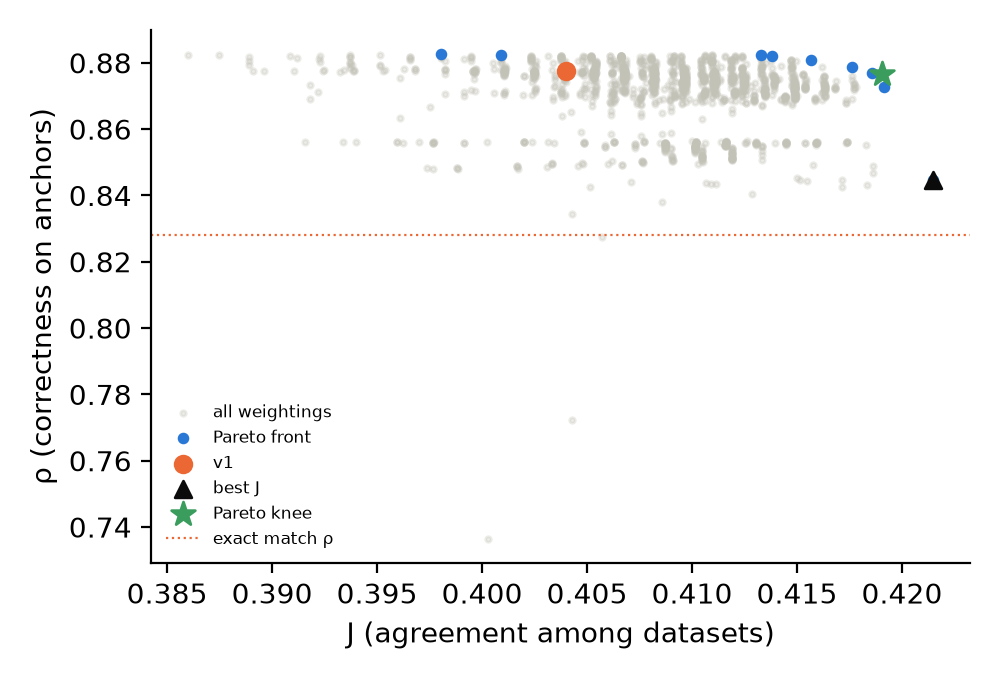
\includegraphics[width=0.75\textwidth]{fig_pareto.png}
\caption{Agreement $J$ against anchor correctness $\rho$ for every weighting; v1, the best-$J$, best-$\rho$ and knee points marked.}
\label{fig:pareto}
\end{figure}
\notable{The cloud is wide in $\rho$ (0.74--0.88) and narrow in $J$ (0.38--0.41), and the two correlate $-0.23$: agreement is not a proxy for correctness. v1 sits on the upper edge near the $\rho$ optimum; recall-only and decay-only, the corners that score well on $J$, are the worst by $\rho$.}

\subsection{Leaderboard}
\inoneline{The ends of the table are certain, the top three reorder with the rule, and Gemini 3.1 Pro lands fifth.}
Under every rule the Friedman test rejects equal models ($p<0.001$) while datasets agree only moderately (Kendall's $W$ 0.26--0.27). The ends of the ranking are stable: Llama 3.3 70B is last and gpt-oss-120b tenth under every rule and every pooling method, with Holm-corrected significance against the top group. The order inside the top three depends on the rule and the pooling method (Tables~\ref{tab:leaderboard_headline} and \ref{tab:ranks_by_rule}, Figure~\ref{fig:leaderboard}): Bradley--Terry puts Gemini 3.8 Flash first under v1 and all calibrated rules, Borda puts GPT-5.5 first under those rules, and exact match puts Claude Opus 5 first under both. Gemini 3.1 Pro, added in this run, lands fifth by Bradley--Terry under v1 and fourth under exact match; DeepSeek-R1 moved up one place after its unfinished answers were re-asked at 16,000 tokens.

\begin{landscape}
\begin{table}[htbp]
\centering\tiny
\caption{Leaderboard under the deployed rule (v1 weights): Bradley--Terry strength $\pm$ SE vs reference with the 95\,\% bootstrap rank interval, Borda rank with its interval, and the mean composite over the suite.}
\label{tab:leaderboard_headline}
\setlength{\tabcolsep}{3pt}
\resizebox{\linewidth}{!}{%
\begin{tabular}{lrrrrrrrrr}
\toprule
rank & model & BT strength & SE & BT 95\% & P(first) BT & Borda rank & Borda 95\% & P(first) Borda & mean score \\
\midrule
1 & Gemini 3.8 Flash & 0.115 & 0.015 & [1, 2] & 0.910 & 3 & [1, 3] & 0.040 & 0.812 \\
2 & Claude Opus 5 & 0.101 & 0.000 & [1, 2] & 0.090 & 2 & [1, 3] & 0.500 & 0.812 \\
3 & GPT-5.5 & 0.045 & 0.015 & [3, 5] & 0.000 & 1 & [1, 3] & 0.440 & 0.808 \\
4 & Claude Sonnet 5 & 0.027 & 0.015 & [3, 6] & 0.000 & 4 & [4, 7] & 0.000 & 0.796 \\
5 & Gemini 3.1 Pro & 0.026 & 0.015 & [3, 6] & 0.000 & 6 & [4, 7] & 0.000 & 0.799 \\
6 & Grok 4 & 0.020 & 0.015 & [4, 6] & 0.000 & 7 & [4, 7] & 0.000 & 0.797 \\
7 & DeepSeek-R1 & -0.007 & 0.015 & [7, 9] & 0.000 & 5 & [4, 8] & 0.000 & 0.794 \\
8 & GPT-5.4-mini & -0.017 & 0.015 & [7, 9] & 0.000 & 9 & [7, 9] & 0.000 & 0.790 \\
9 & DeepSeek-chat & -0.026 & 0.015 & [7, 9] & 0.000 & 8 & [7, 9] & 0.000 & 0.784 \\
10 & gpt-oss-120b & -0.107 & 0.015 & [10, 10] & 0.000 & 10 & [10, 11] & 0.000 & 0.767 \\
11 & Llama 3.3 70B & -0.177 & 0.015 & [11, 11] & 0.000 & 11 & [10, 11] & 0.000 & 0.738 \\
\bottomrule
\end{tabular}
}
\end{table}
\end{landscape}

\notable{Gemini 3.8 Flash is first by Bradley--Terry with $P(\text{first}) = 0.91$ because it wins many items by small margins; by Borda, which counts dataset-level ranks, GPT-5.5 is first and Flash third. The bottom two (gpt-oss-120b, Llama 3.3 70B) have rank intervals of width zero; ranks 4--9 overlap and are not established.}
\begin{landscape}
\begin{table}[htbp]
\centering\tiny
\caption{Bradley--Terry rank (Borda rank in brackets) under each reported rule, with the Friedman $p$ and Kendall's $W$ among datasets.}
\label{tab:ranks_by_rule}
\setlength{\tabcolsep}{3pt}
\resizebox{\linewidth}{!}{%
\begin{tabular}{lrrrrrrrrrrrrr}
\toprule
rule & Gemini 3.8 Flash & Claude Opus 5 & GPT-5.5 & Claude Sonnet 5 & Gemini 3.1 Pro & Grok 4 & DeepSeek-R1 & GPT-5.4-mini & DeepSeek-chat & gpt-oss-120b & Llama 3.3 70B & Friedman p & W \\
\midrule
exact match & 3 (3) & 1 (1) & 2 (2) & 7 (4) & 4 (7) & 5 (6) & 6 (5) & 8 (9) & 9 (8) & 10 (10) & 11 (11) & 1.3e-14 & 0.27 \\
v1 & 1 (3) & 2 (2) & 3 (1) & 4 (4) & 5 (6) & 6 (7) & 7 (5) & 8 (9) & 9 (8) & 10 (10) & 11 (11) & 1.5e-13 & 0.26 \\
top1 & 1 (3) & 2 (2) & 3 (1) & 4 (4) & 5 (5) & 6 (5) & 7 (7) & 8 (8) & 9 (9) & 10 (10) & 11 (11) & 6.8e-14 & 0.26 \\
top2 & 1 (3) & 3 (1) & 2 (2) & 7 (5) & 4 (4) & 5 (6) & 6 (7) & 9 (9) & 8 (8) & 10 (10) & 11 (11) & 1.0e-13 & 0.26 \\
top3 & 1 (3) & 3 (1) & 2 (2) & 7 (5) & 4 (4) & 5 (6) & 6 (7) & 9 (9) & 8 (8) & 10 (10) & 11 (11) & 1.0e-13 & 0.26 \\
top4 & 1 (3) & 3 (1) & 2 (2) & 7 (5) & 4 (4) & 6 (7) & 5 (5) & 9 (9) & 8 (8) & 10 (10) & 11 (11) & 8.0e-14 & 0.26 \\
top5 & 1 (3) & 2 (1) & 3 (2) & 4 (6) & 5 (6) & 6 (5) & 7 (4) & 9 (9) & 8 (8) & 10 (10) & 11 (11) & 4.3e-14 & 0.27 \\
best-rho & 1 (3) & 2 (2) & 3 (1) & 4 (4) & 5 (5) & 7 (7) & 8 (6) & 6 (8) & 9 (9) & 10 (10) & 11 (11) & 7.2e-13 & 0.25 \\
knee & 1 (3) & 2 (2) & 3 (1) & 4 (4) & 5 (5) & 6 (5) & 7 (7) & 8 (8) & 9 (9) & 10 (10) & 11 (11) & 6.8e-14 & 0.26 \\
\bottomrule
\end{tabular}
}
\end{table}
\end{landscape}

\notable{Rows 10 and 11 never move; the top three permute with the rule (exact match favours Opus, every graded rule favours Flash by Bradley--Terry and GPT-5.5 by Borda). Gemini 3.1 Pro is fourth or fifth under every rule (fourth under exact match and the second to fourth $J$ weightings, fifth otherwise); DeepSeek-R1 sits fifth to eighth, seventh under v1, after its 16,000-token re-asks. Kendall's $W$ among datasets is 0.26--0.27 under every rule.}

\begin{figure}[htbp]
\centering
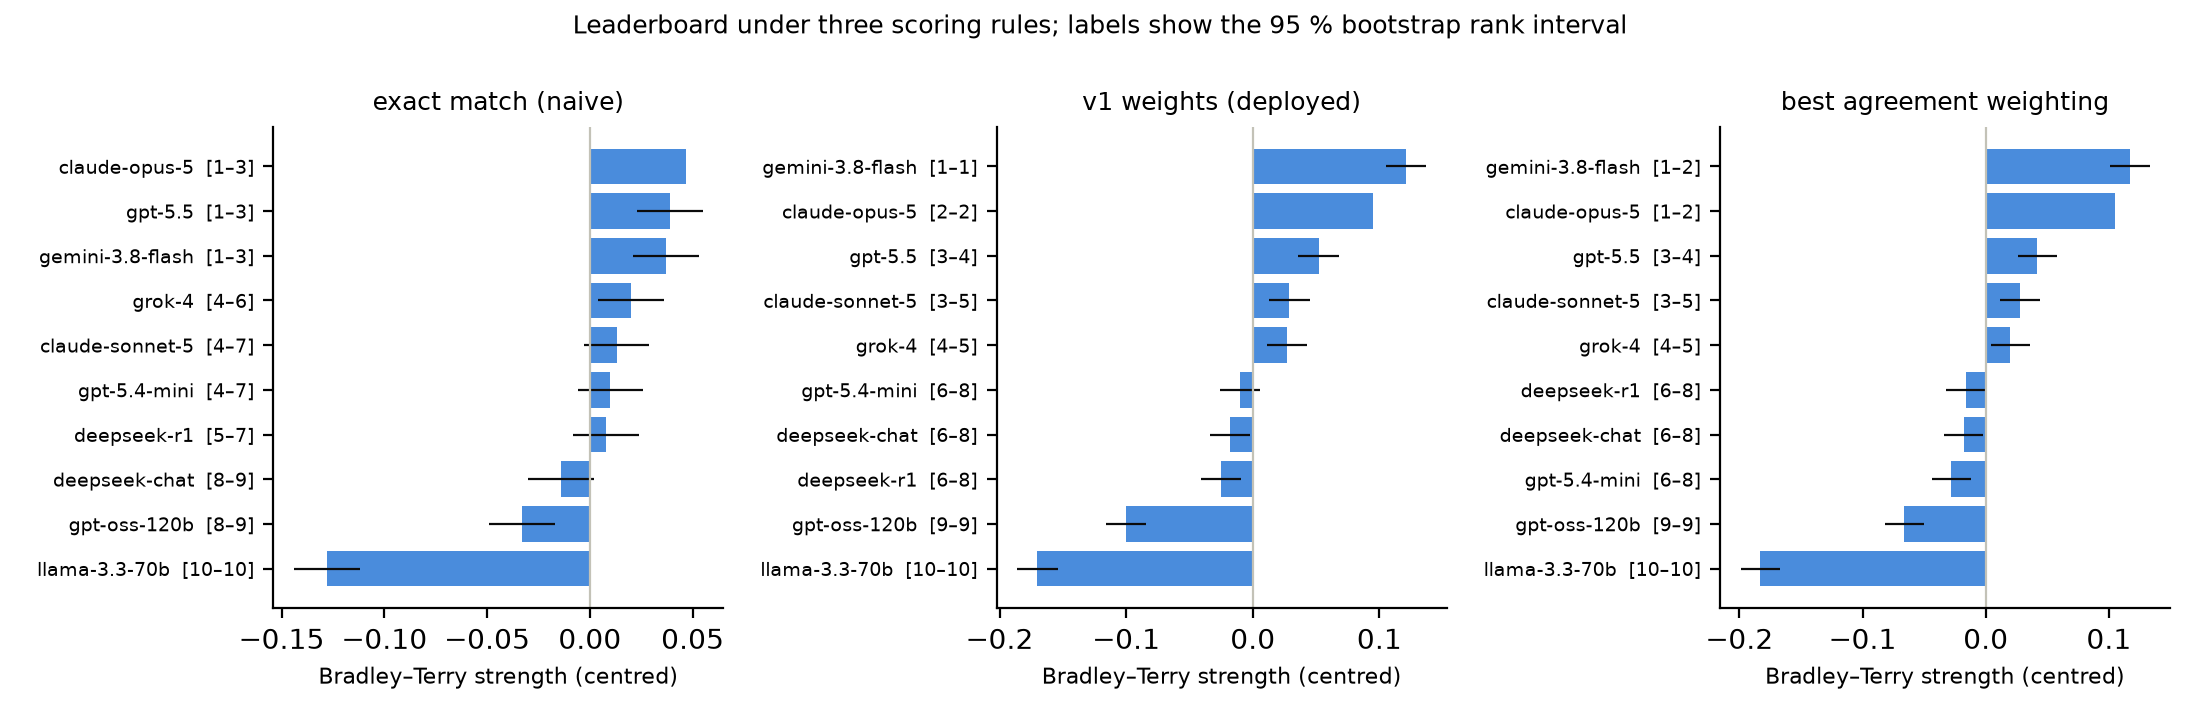
\includegraphics[width=0.95\textwidth]{fig_leaderboard_rules.png}
\caption{Bradley--Terry strengths $\pm$ SE with bootstrap rank intervals under exact match, v1 and the best-$J$ weighting. The ends are stable; the top order is rule-dependent.}
\label{fig:leaderboard}
\end{figure}
\notable{The strengths of ranks 4--9 lie within about 0.05 of each other with overlapping error bars; the gap from rank 9 to rank 10 and from 10 to 11 is larger than the whole middle band. The figure is the visual form of the Holm result: 15 of 55 pairs significant, all of them against the bottom two models.}

\begin{figure}[htbp]
\centering
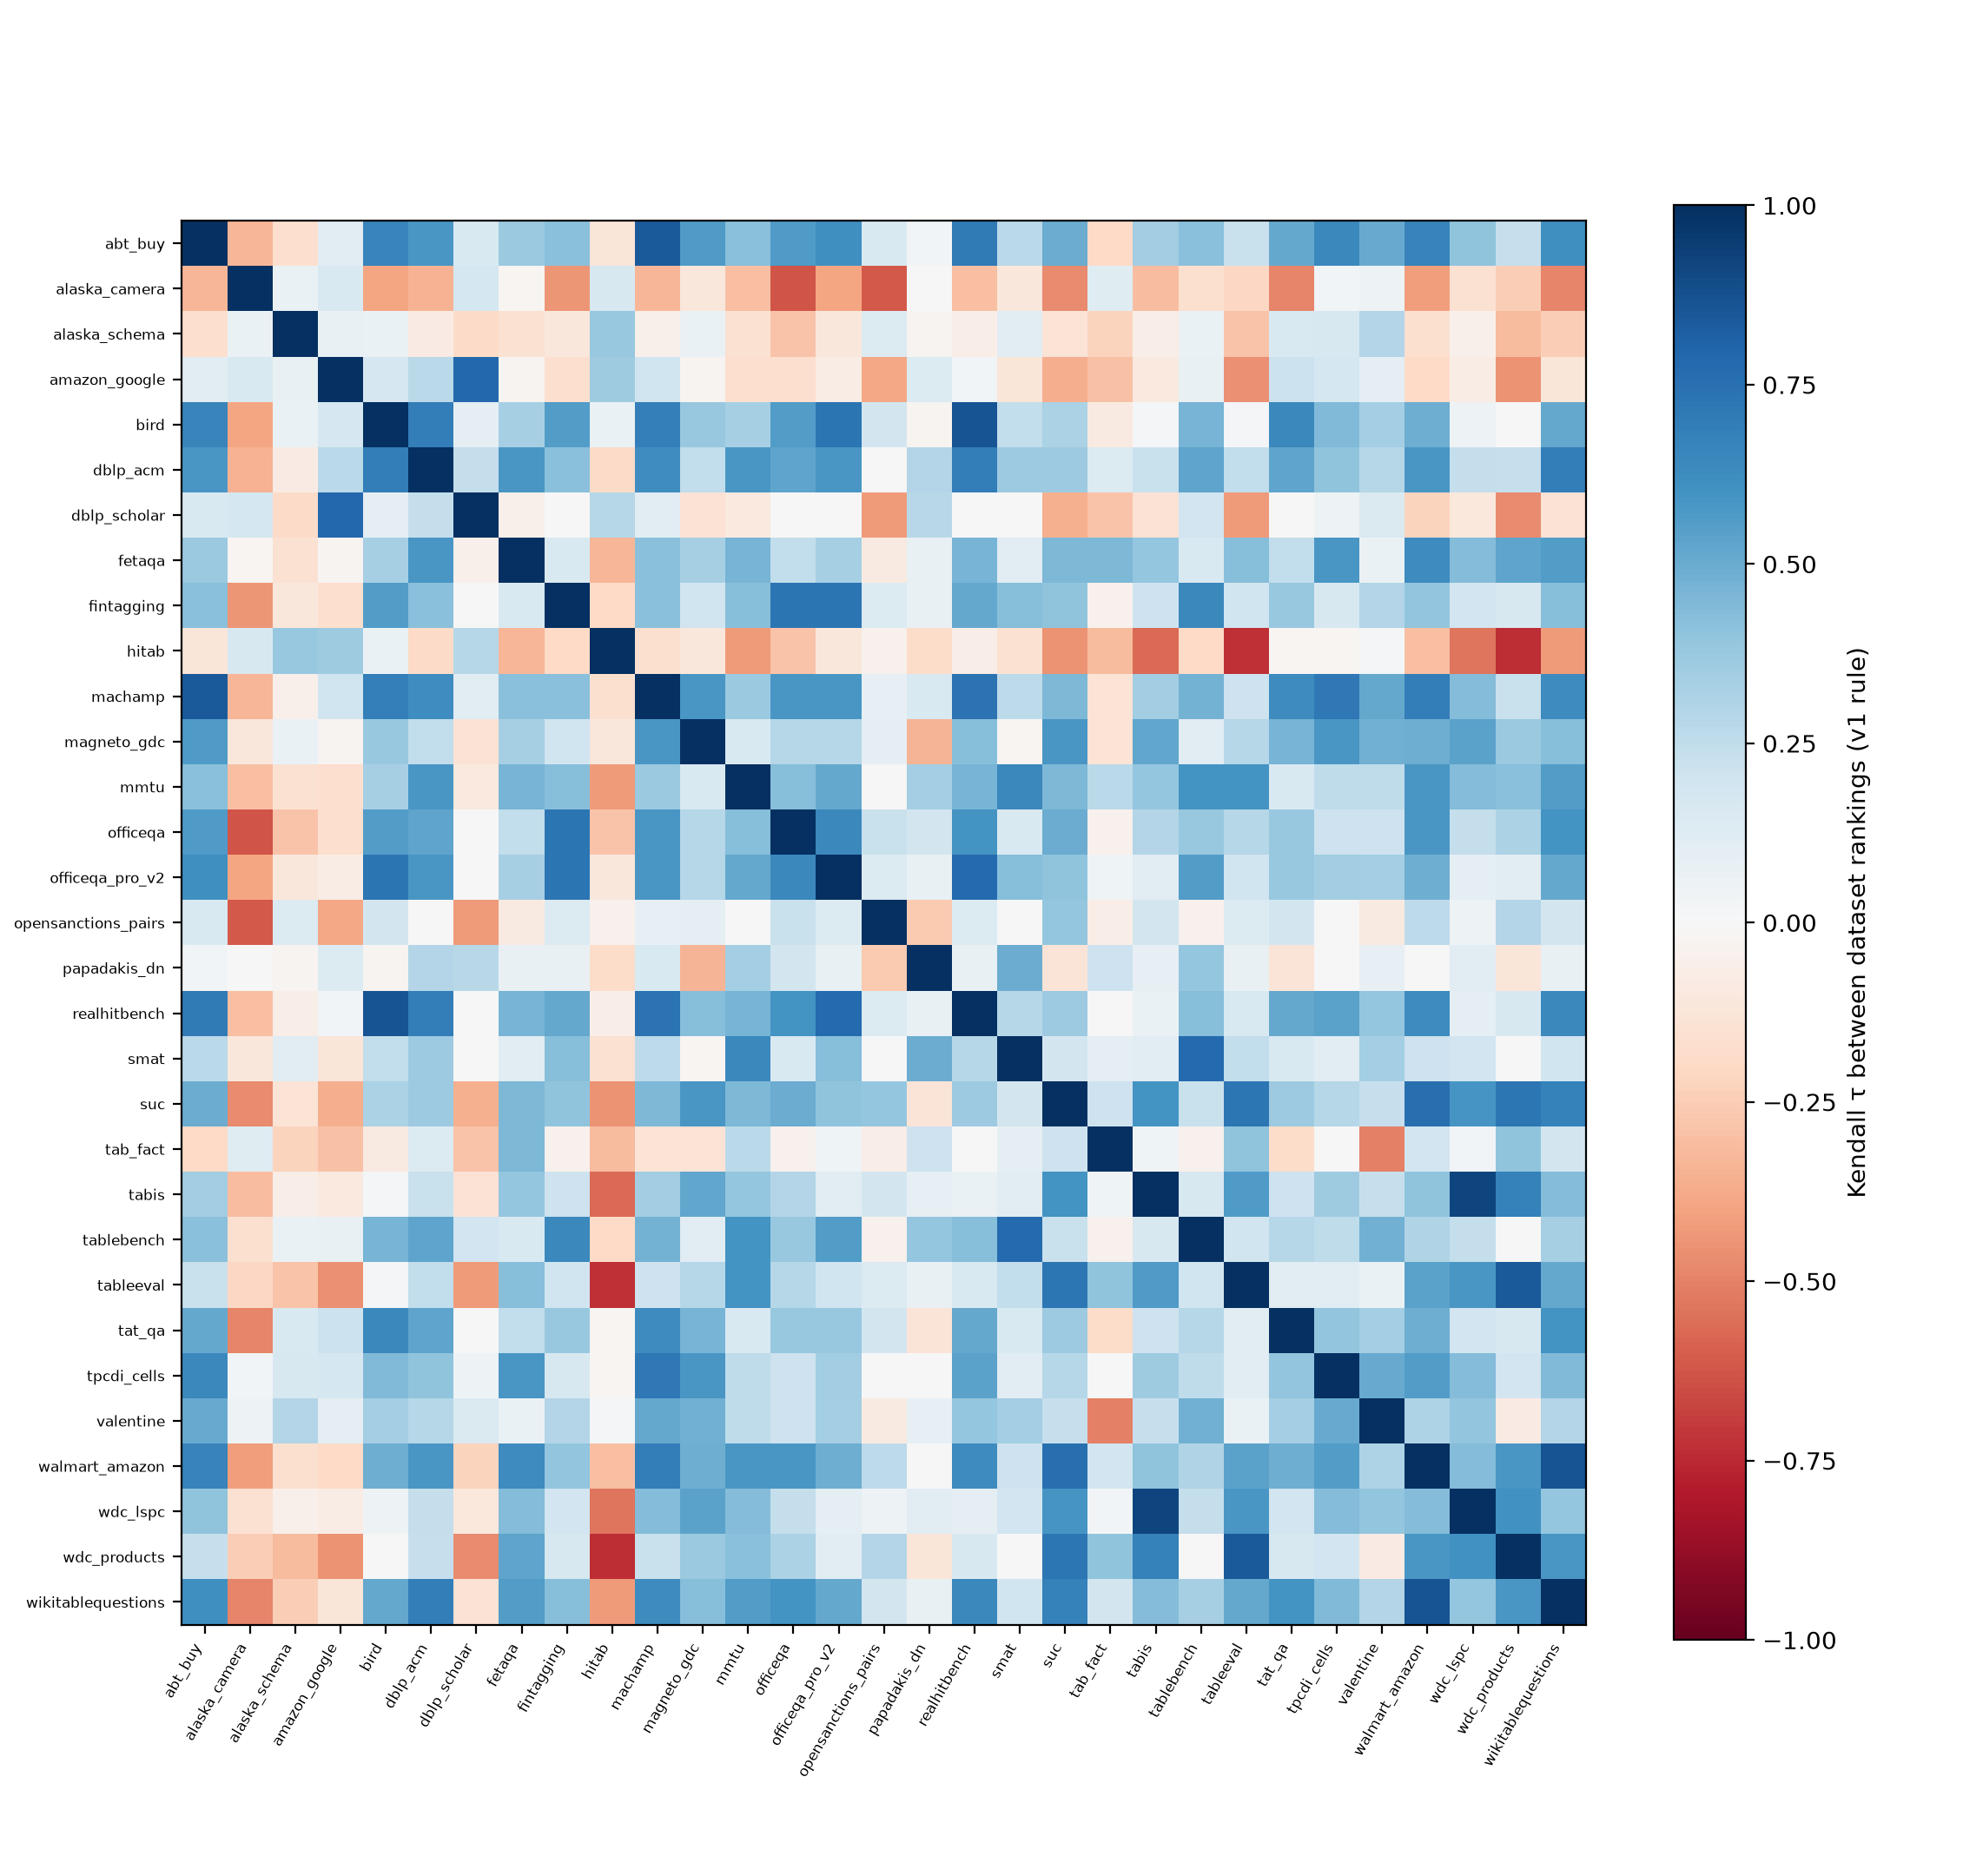
\includegraphics[width=0.8\textwidth]{fig_dataset_tau.png}
\caption{Kendall $\tau$ between the model rankings of each pair of datasets under v1. Datasets agree only moderately ($W\approx0.26$).}
\label{fig:dataset_tau}
\end{figure}
\notable{Blue blocks sit inside families and the finance and table-QA sets agree with most of the suite; Alaska Camera and HiTab are red against almost everyone. The leaderboard is an average over datasets that disagree about the middle of the table, which is what $W = 0.26$ says in one number.}

\subsection{Comparability with published numbers}
\inoneline{Accuracy survives re-weighting to the official splits; balanced-pool F1 on sparse matching sets does not.}
Post-stratification to the official split changes dataset accuracy by at most 0.09 (OpenSanctions pairs). For the matching sets, positive-class F1 computed on the balanced 50/50 pool overstates F1 at the official match ratio wherever the official split is sparse, by up to 0.19 on Amazon--Google (Table~\ref{tab:official_split_by_dataset}, Figure~\ref{fig:official}).

\begin{table}[htbp]
\centering\tiny
\caption{Official-split estimates under v1 averaged over the ten models.}
\label{tab:official_split_by_dataset}
\setlength{\tabcolsep}{3pt}
\begin{tabular}{p{0.112\linewidth}p{0.063\linewidth}p{0.081\linewidth}p{0.104\linewidth}p{0.130\linewidth}p{0.123\linewidth}p{0.112\linewidth}p{0.133\linewidth}}
\toprule
dataset & suite\_\allowbreak{}mean & official\_\allowbreak{}estimate & suite\_\allowbreak{}f1\_\allowbreak{}pos & official\_\allowbreak{}precision\_\allowbreak{}pos & official\_\allowbreak{}recall\_\allowbreak{}pos & official\_\allowbreak{}f1\_\allowbreak{}pos & official\_\allowbreak{}positive\_\allowbreak{}share \\
\midrule
abt\_\allowbreak{}buy & 0.970 & 0.986 & 0.968 & 0.926 & 0.949 & 0.936 & 0.108 \\
alaska\_\allowbreak{}camera & 0.958 & 0.958 & 0.955 & 1.000 & 0.921 & 0.955 & 0.500 \\
alaska\_\allowbreak{}schema & 0.928 & 0.928 & -- & -- & -- & -- & -- \\
amazon\_\allowbreak{}google & 0.936 & 0.932 & 0.929 & 0.611 & 0.942 & 0.739 & 0.102 \\
bird & 0.187 & 0.213 & -- & -- & -- & -- & -- \\
dblp\_\allowbreak{}acm & 0.986 & 0.991 & 0.985 & 0.979 & 0.978 & 0.976 & 0.180 \\
dblp\_\allowbreak{}scholar & 0.949 & 0.966 & 0.948 & 0.900 & 0.924 & 0.910 & 0.186 \\
fetaqa & 0.382 & 0.382 & -- & -- & -- & -- & -- \\
fintagging & 0.880 & 0.876 & -- & -- & -- & -- & -- \\
hitab & 0.770 & 0.773 & -- & -- & -- & -- & -- \\
machamp & 0.887 & 0.890 & 0.892 & 0.644 & 0.853 & 0.733 & 0.175 \\
magneto\_\allowbreak{}gdc & 0.934 & 0.938 & -- & -- & -- & -- & -- \\
mmtu & 0.867 & 0.829 & -- & -- & -- & -- & -- \\
officeqa & 0.129 & 0.129 & -- & -- & -- & -- & -- \\
officeqa\_\allowbreak{}pro\_\allowbreak{}v2 & 0.139 & 0.139 & -- & -- & -- & -- & -- \\
opensanctions\_\allowbreak{}pairs & 0.821 & 0.727 & 0.773 & 0.993 & 0.649 & 0.777 & 0.769 \\
papadakis\_\allowbreak{}dn & 0.941 & 0.988 & 0.833 & 0.550 & 0.963 & 0.683 & 0.018 \\
realhitbench & 0.673 & 0.673 & -- & -- & -- & -- & -- \\
smat & 0.918 & 0.916 & -- & -- & -- & -- & -- \\
suc & 0.914 & 0.912 & -- & -- & -- & -- & -- \\
tab\_\allowbreak{}fact & 0.798 & 0.789 & 0.758 & 0.896 & 0.674 & 0.764 & 0.500 \\
tabis & 0.915 & 0.918 & -- & -- & -- & -- & -- \\
tablebench & 0.818 & 0.816 & -- & -- & -- & -- & -- \\
tableeval & 0.749 & 0.754 & -- & -- & -- & -- & -- \\
tat\_\allowbreak{}qa & 0.803 & 0.758 & -- & -- & -- & -- & -- \\
tpcdi\_\allowbreak{}cells & 0.456 & 0.461 & -- & -- & -- & -- & -- \\
valentine & 0.984 & 0.979 & -- & -- & -- & -- & -- \\
walmart\_\allowbreak{}amazon & 0.958 & 0.975 & 0.947 & 0.832 & 0.927 & 0.875 & 0.094 \\
wdc\_\allowbreak{}lspc & 0.982 & 0.983 & 0.983 & 0.965 & 0.979 & 0.971 & 0.264 \\
wdc\_\allowbreak{}products & 0.978 & 0.985 & 0.979 & 0.980 & 0.968 & 0.974 & 0.280 \\
wikitablequestions & 0.846 & 0.844 & -- & -- & -- & -- & -- \\
\bottomrule
\end{tabular}
\end{table}

\notable{Accuracy moves by at most 0.09 (OpenSanctions, whose official class ratio is 0.77 rather than 0.5). Positive-class F1 drops by 0.19 on Amazon--Google, 0.17 on Papadakis--Christen and 0.16 on Machamp, all through precision: at a 2--10\,\% official match rate a 1\,\% false-positive rate costs more than any recall gain.}

\begin{figure}[htbp]
\centering
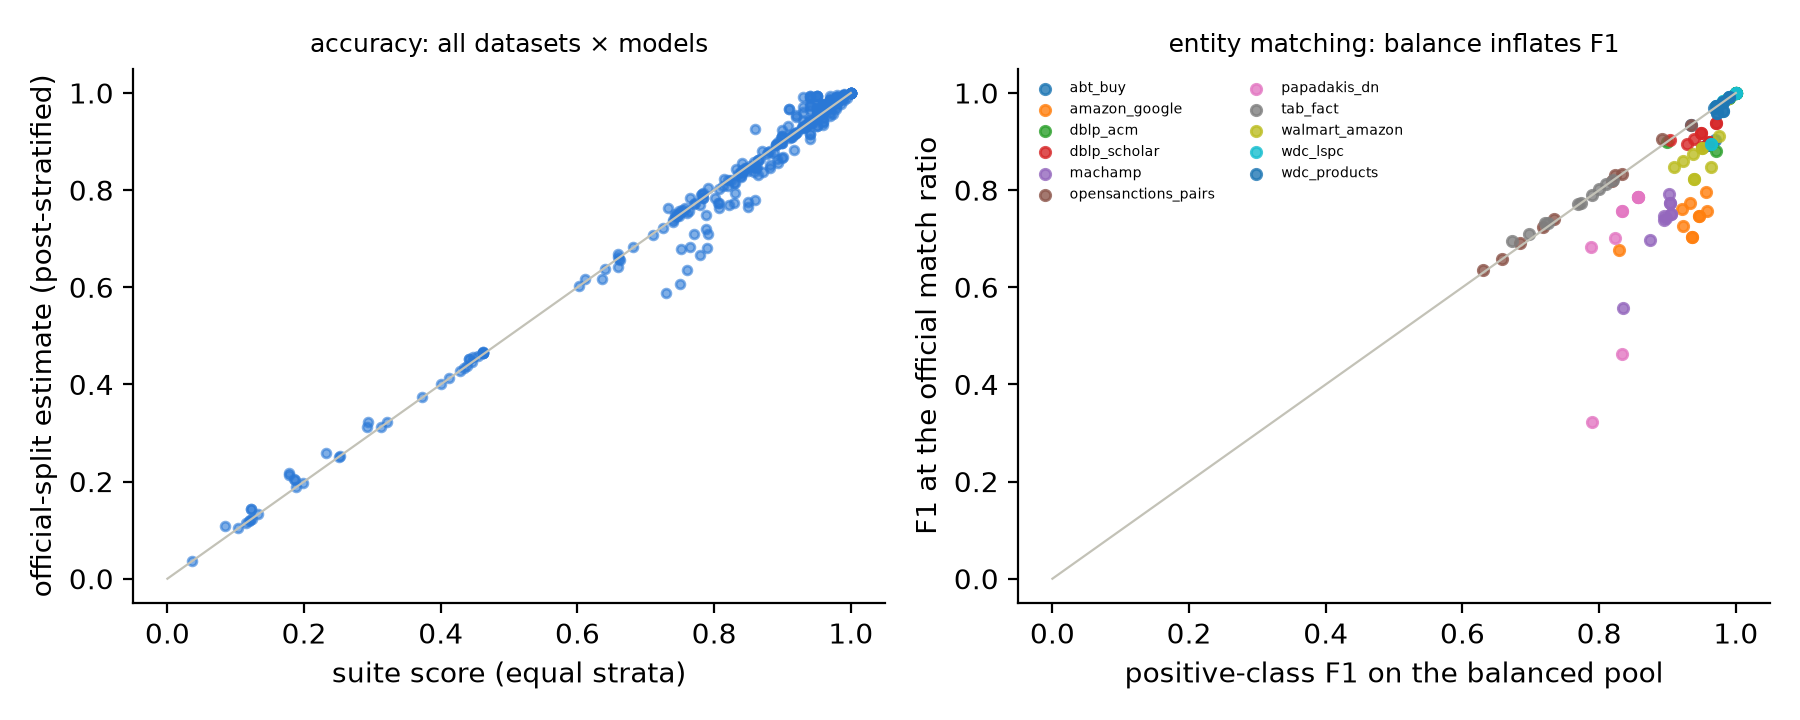
\includegraphics[width=0.9\textwidth]{fig_official_split.png}
\caption{Suite score vs post-stratified official estimate per dataset, and matching F1 on the balanced pool vs at the official match ratio.}
\label{fig:official}
\end{figure}
\notable{Almost every (dataset, model) point lies on the diagonal for accuracy; the sparse matching sets fall below it for F1. Model order is preserved after re-weighting; the absolute numbers are not, so the official-ratio column is the one to compare with published results.}

\subsection{Dataset diagnostics}
\inoneline{Three sets are at ceiling and twelve separate no model pair; a dozen table and document sets carry the result.}
Three datasets sit at ceiling (mean composite 0.98 with a spread of 0.02--0.04 across models): Valentine, WDC LSPC and WDC Products. They are flagged and remain inside the objective in this run. Two sit near floor for every model (OfficeQA closed-book and OfficeQA Pro V2) and one is a known hard set (BIRD); none is excluded. Self-stability $\tau$ (rank agreement between bootstrap halves of a dataset) ranges from 0.57 to 0.92. Twelve datasets, all the entity-matching sets plus Valentine and TPC-DI, separate no model pair at the item level; four separate twenty or more.

\clearpage
\appendix
\section{All figures, with a reading guide}
\label{app:figures}
Every figure that can be drawn from the saved outputs, each followed by what it encodes, how to read it and what it shows. Source data for each is in \texttt{data/}.

\begin{figure}[htbp]\centering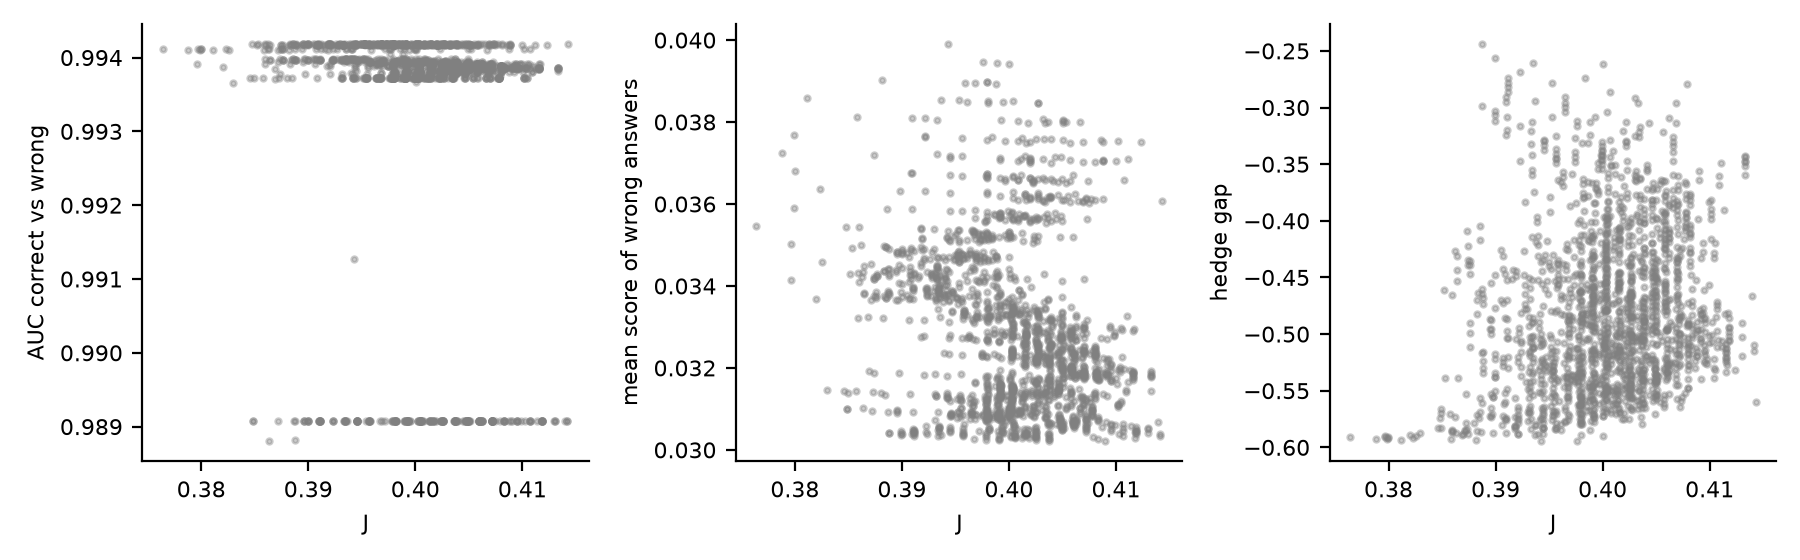
\includegraphics[width=0.9\textwidth]{fig_anchor_metrics_vs_j.png}\caption{Three further anchor diagnostics against $J$ for every weighting.}\label{figall:fig_anchor_metrics_vs_j}\end{figure}
\noindent{\small \textbf{What it encodes.} Three anchor diagnostics against $J$ for every weighting: AUC for separating correct from wrong anchors, the mean score given to wrong anchors, and the hedge gap (score of a committed answer minus the same answer hedged). \textbf{How to read it.} Flat clouds mean the diagnostic does not depend on the weighting; a slope means agreement trades against it. \textbf{What it shows.} AUC is 0.989--0.994 for every weighting: all separate right from wrong. Wrong answers score below 0.06 everywhere. The differences between weightings are in partial credit, not in discrimination.}
\clearpage

\begin{figure}[htbp]\centering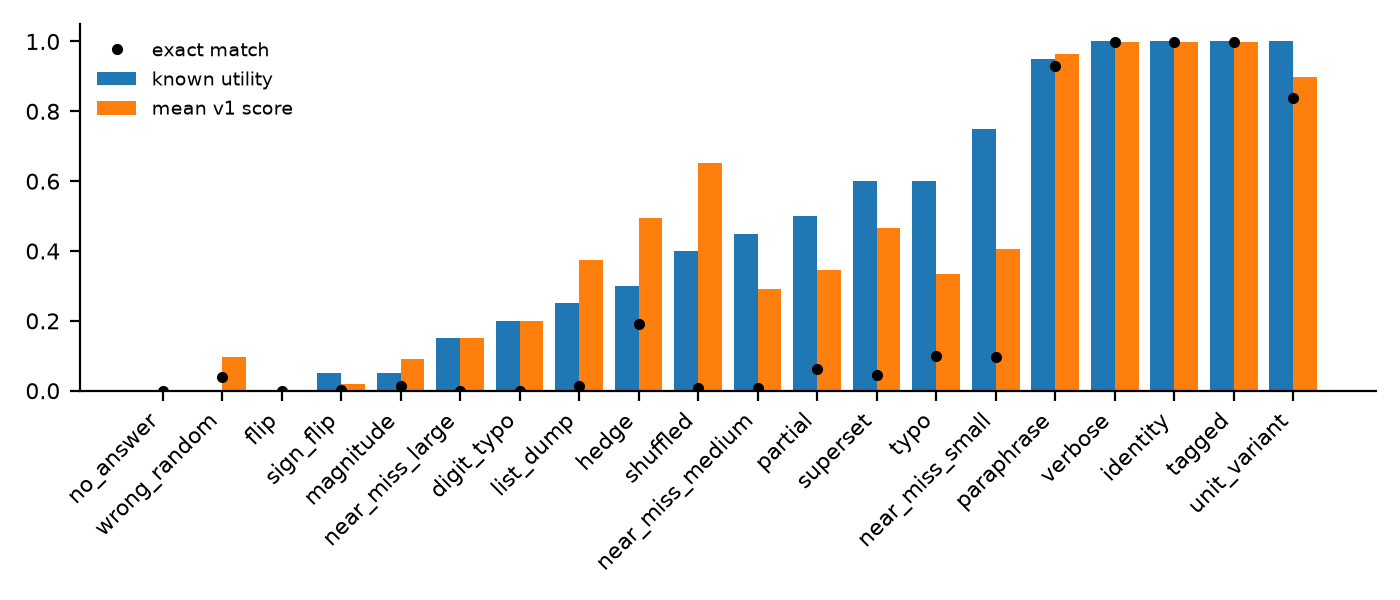
\includegraphics[width=0.9\textwidth]{fig_anchor_operators.png}\caption{Synthetic anchors: known utility of each perturbation operator against the mean v1 score and exact match it receives.}\label{figall:fig_anchor_operators}\end{figure}
\noindent{\small \textbf{What it encodes.} Each anchor operator (a typed perturbation applied to gold answers) with its assigned utility, the mean v1 score it receives, and its exact-match rate. \textbf{How to read it.} A perfect judge would put the blue point on the grey one for every operator. Blue above grey is over-generosity, blue below is over-severity. \textbf{What it shows.} The ends are right (identity, verbose and tagged score 1; flips and non-answers score 0). The judge is generous to shuffled lists, supersets and list dumps (token overlap rewards extra correct tokens) and severe on typos, digit typos and medium near misses. These operators are where a human label would disagree with any lexical rule.}
\clearpage

\begin{figure}[htbp]\centering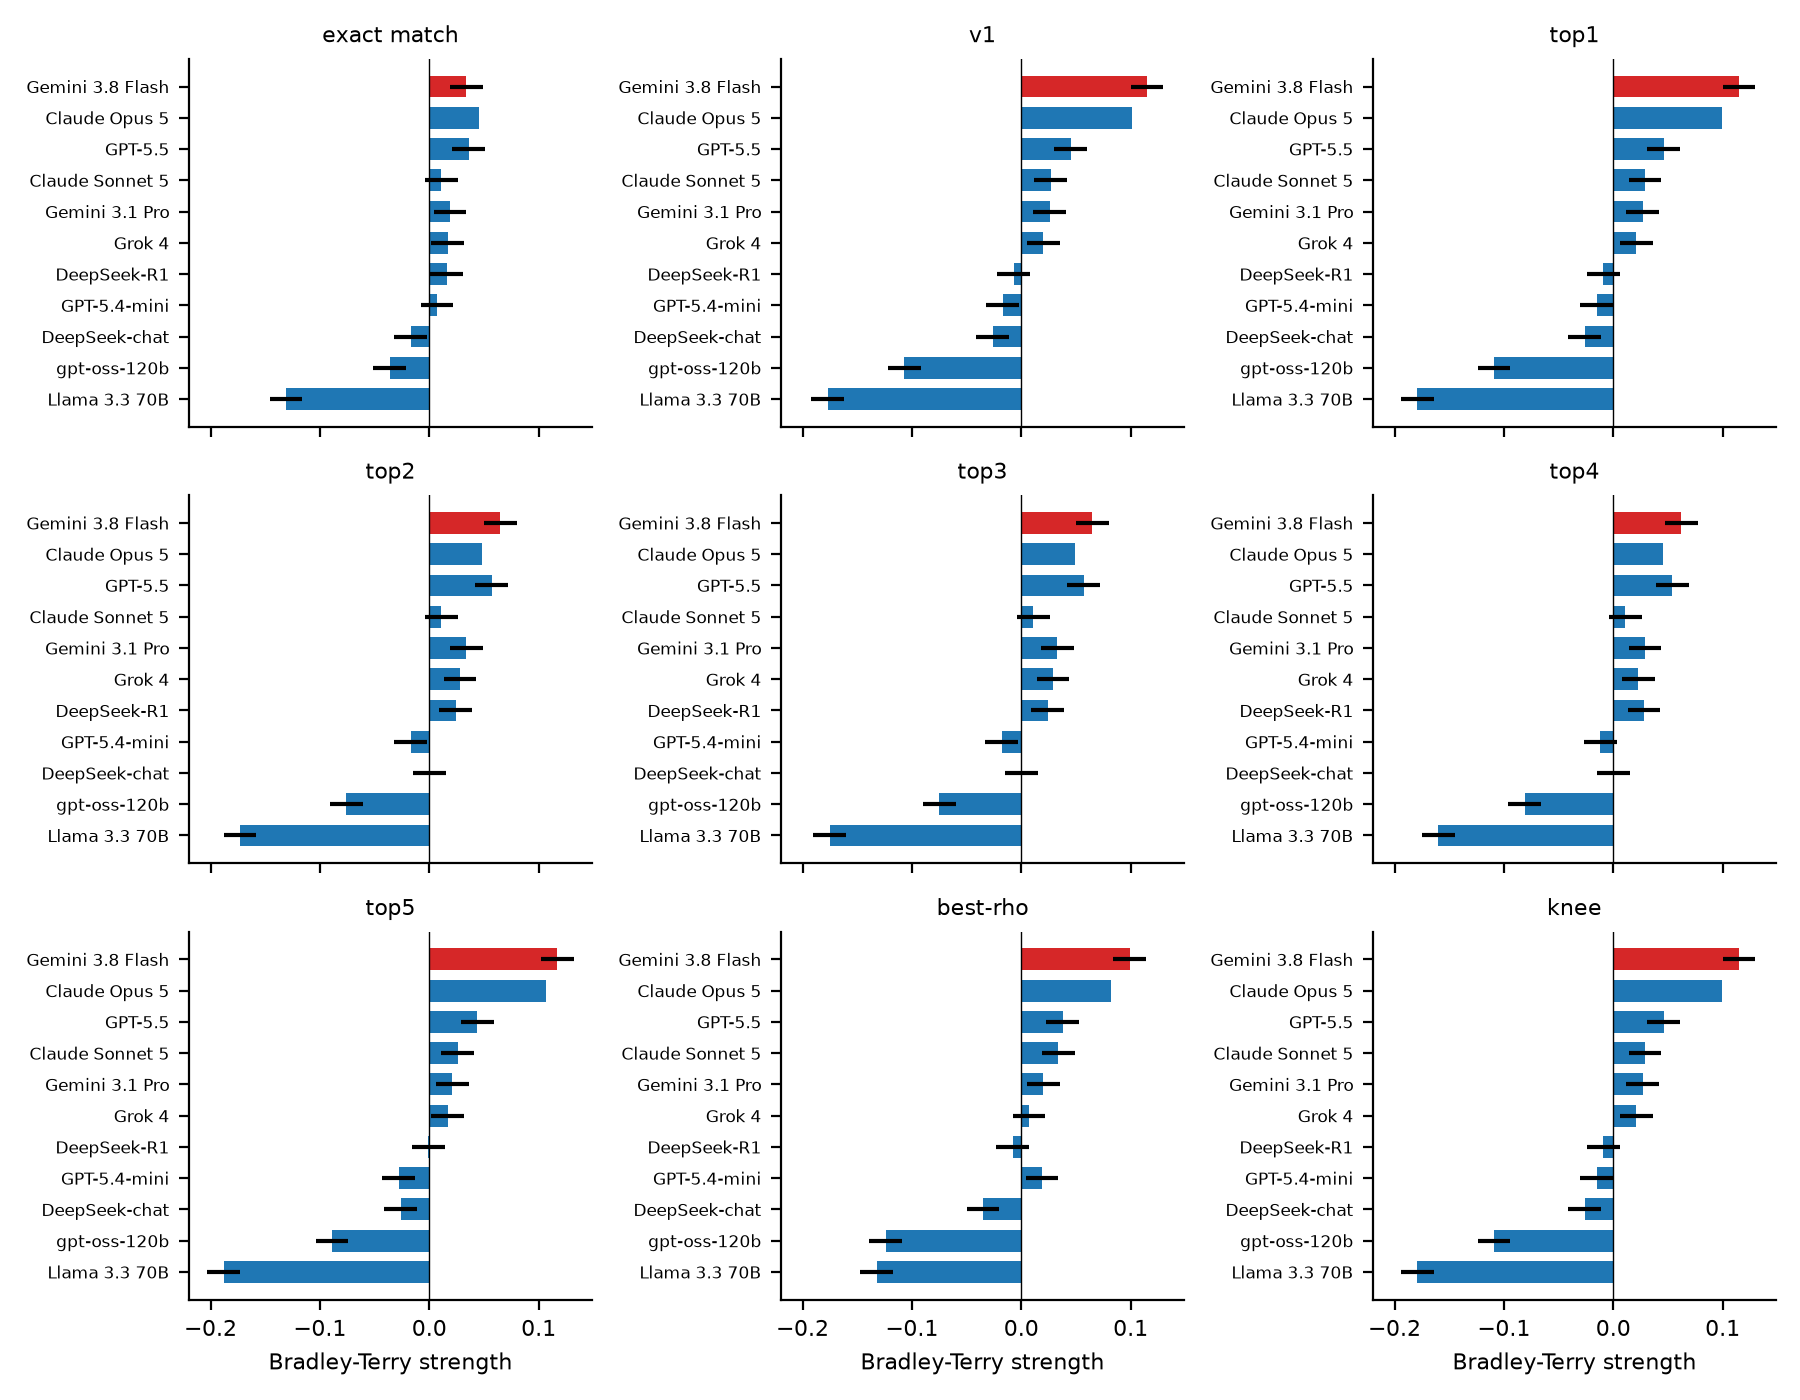
\includegraphics[width=0.9\textwidth]{fig_bt_all_rules.png}\caption{Bradley--Terry strengths ($\pm$ SE vs reference) under every reported rule; models fixed in v1 order.}\label{figall:fig_bt_all_rules}\end{figure}
\noindent{\small \textbf{What it encodes.} Nine small panels, one per reported rule (exact match, v1, the five best by $J$, the best by $\rho$, the Pareto knee), each showing Bradley--Terry strength $\pm$ SE for the ten models in a fixed order; the first-placed model is orange. \textbf{How to read it.} Scan a row across panels to see whether a model's strength is stable; scan the orange markers to see who is first under which rule. \textbf{What it shows.} Rows 4--10 barely move; first place is Opus under exact match and Gemini Flash under every graded rule. Kendall $\tau$ between the rules' rankings is 0.71--1.00.}
\clearpage

\begin{figure}[htbp]\centering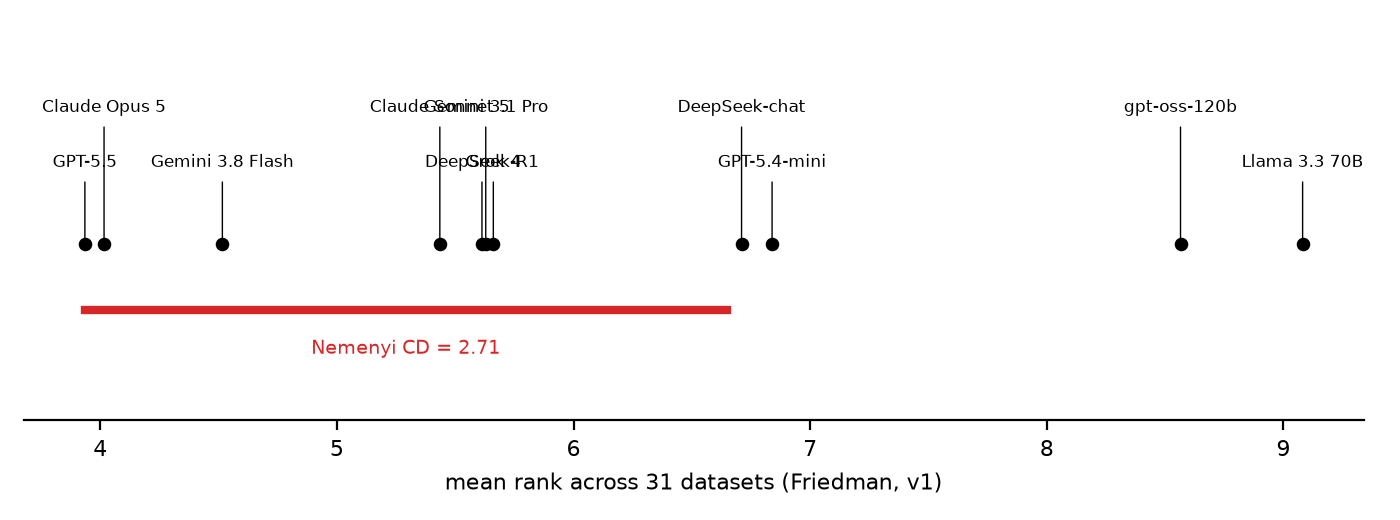
\includegraphics[width=0.9\textwidth]{fig_cd_diagram_v1.png}\caption{Critical-difference view of the Friedman test under v1: mean rank per model and the Nemenyi critical difference at $\alpha = .05$.}\label{figall:fig_cd_diagram_v1}\end{figure}
\noindent{\small \textbf{What it encodes.} The Friedman test's mean rank of each model across the 31 datasets on a single axis, with the Nemenyi critical difference (2.71) drawn as a bar; models closer than the critical difference are not separated at $\alpha$ = .05. \textbf{How to read it.} Two models are significantly different only if their positions differ by more than the bar's length. \textbf{What it shows.} The top group is separated from the bottom two; nothing inside the top group, and nothing in the middle, is separated. With 31 datasets and eleven models this is the resolution the cross-dataset test can offer.}
\clearpage

\begin{figure}[htbp]\centering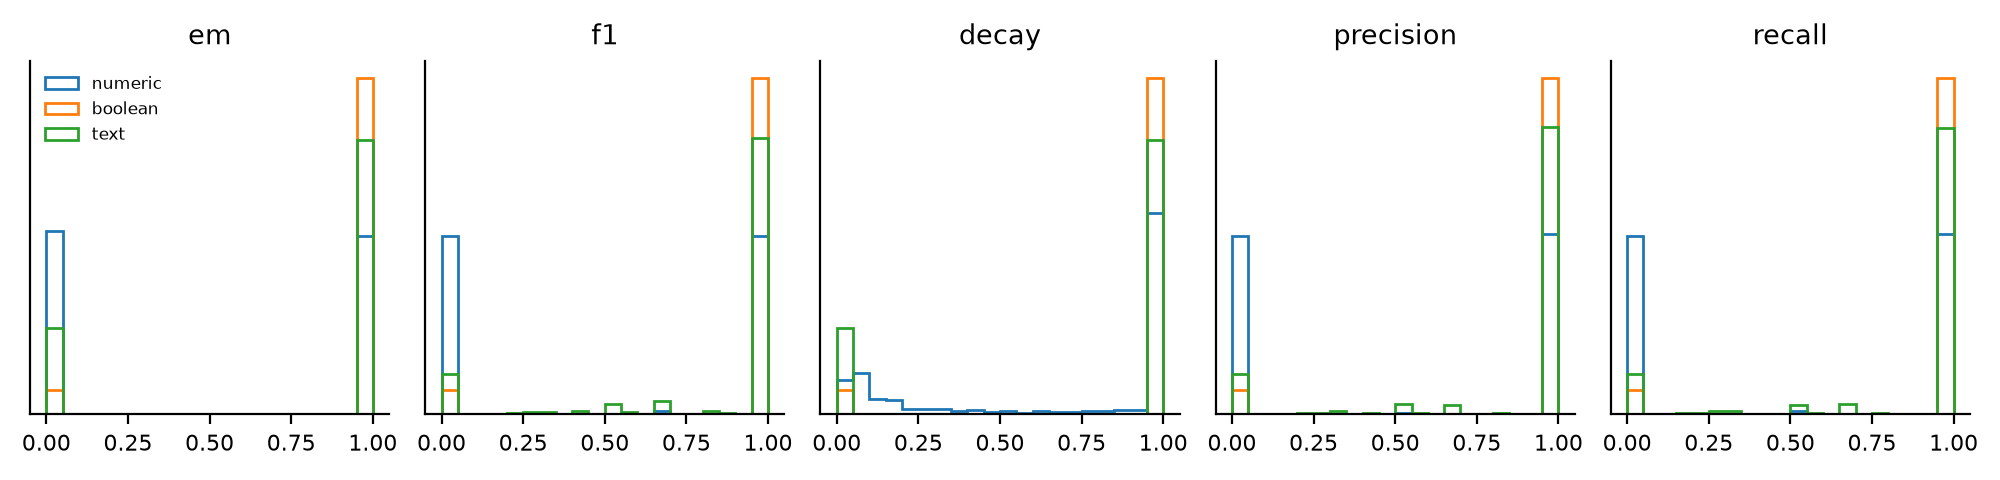
\includegraphics[width=0.9\textwidth]{fig_component_distributions.png}\caption{Distribution of each v1 ingredient over all answers, by answer type.}\label{figall:fig_component_distributions}\end{figure}
\noindent{\small \textbf{What it encodes.} Five panels (exact match, F1, decay, precision, recall); within each, one density curve per answer type (numeric, boolean, text, free-form). \textbf{How to read it.} A curve concentrated at 0 and 1 means the ingredient behaves like a binary score on that answer type; mass in between is graded credit. \textbf{What it shows.} On boolean and text golds every ingredient is binary and identical to exact match. Decay is graded only on numeric golds; F1, precision and recall are graded only on free-form and some text golds. This is the mechanical reason the weights barely matter: the ingredients differ on a minority of answers.}
\clearpage

\begin{figure}[htbp]\centering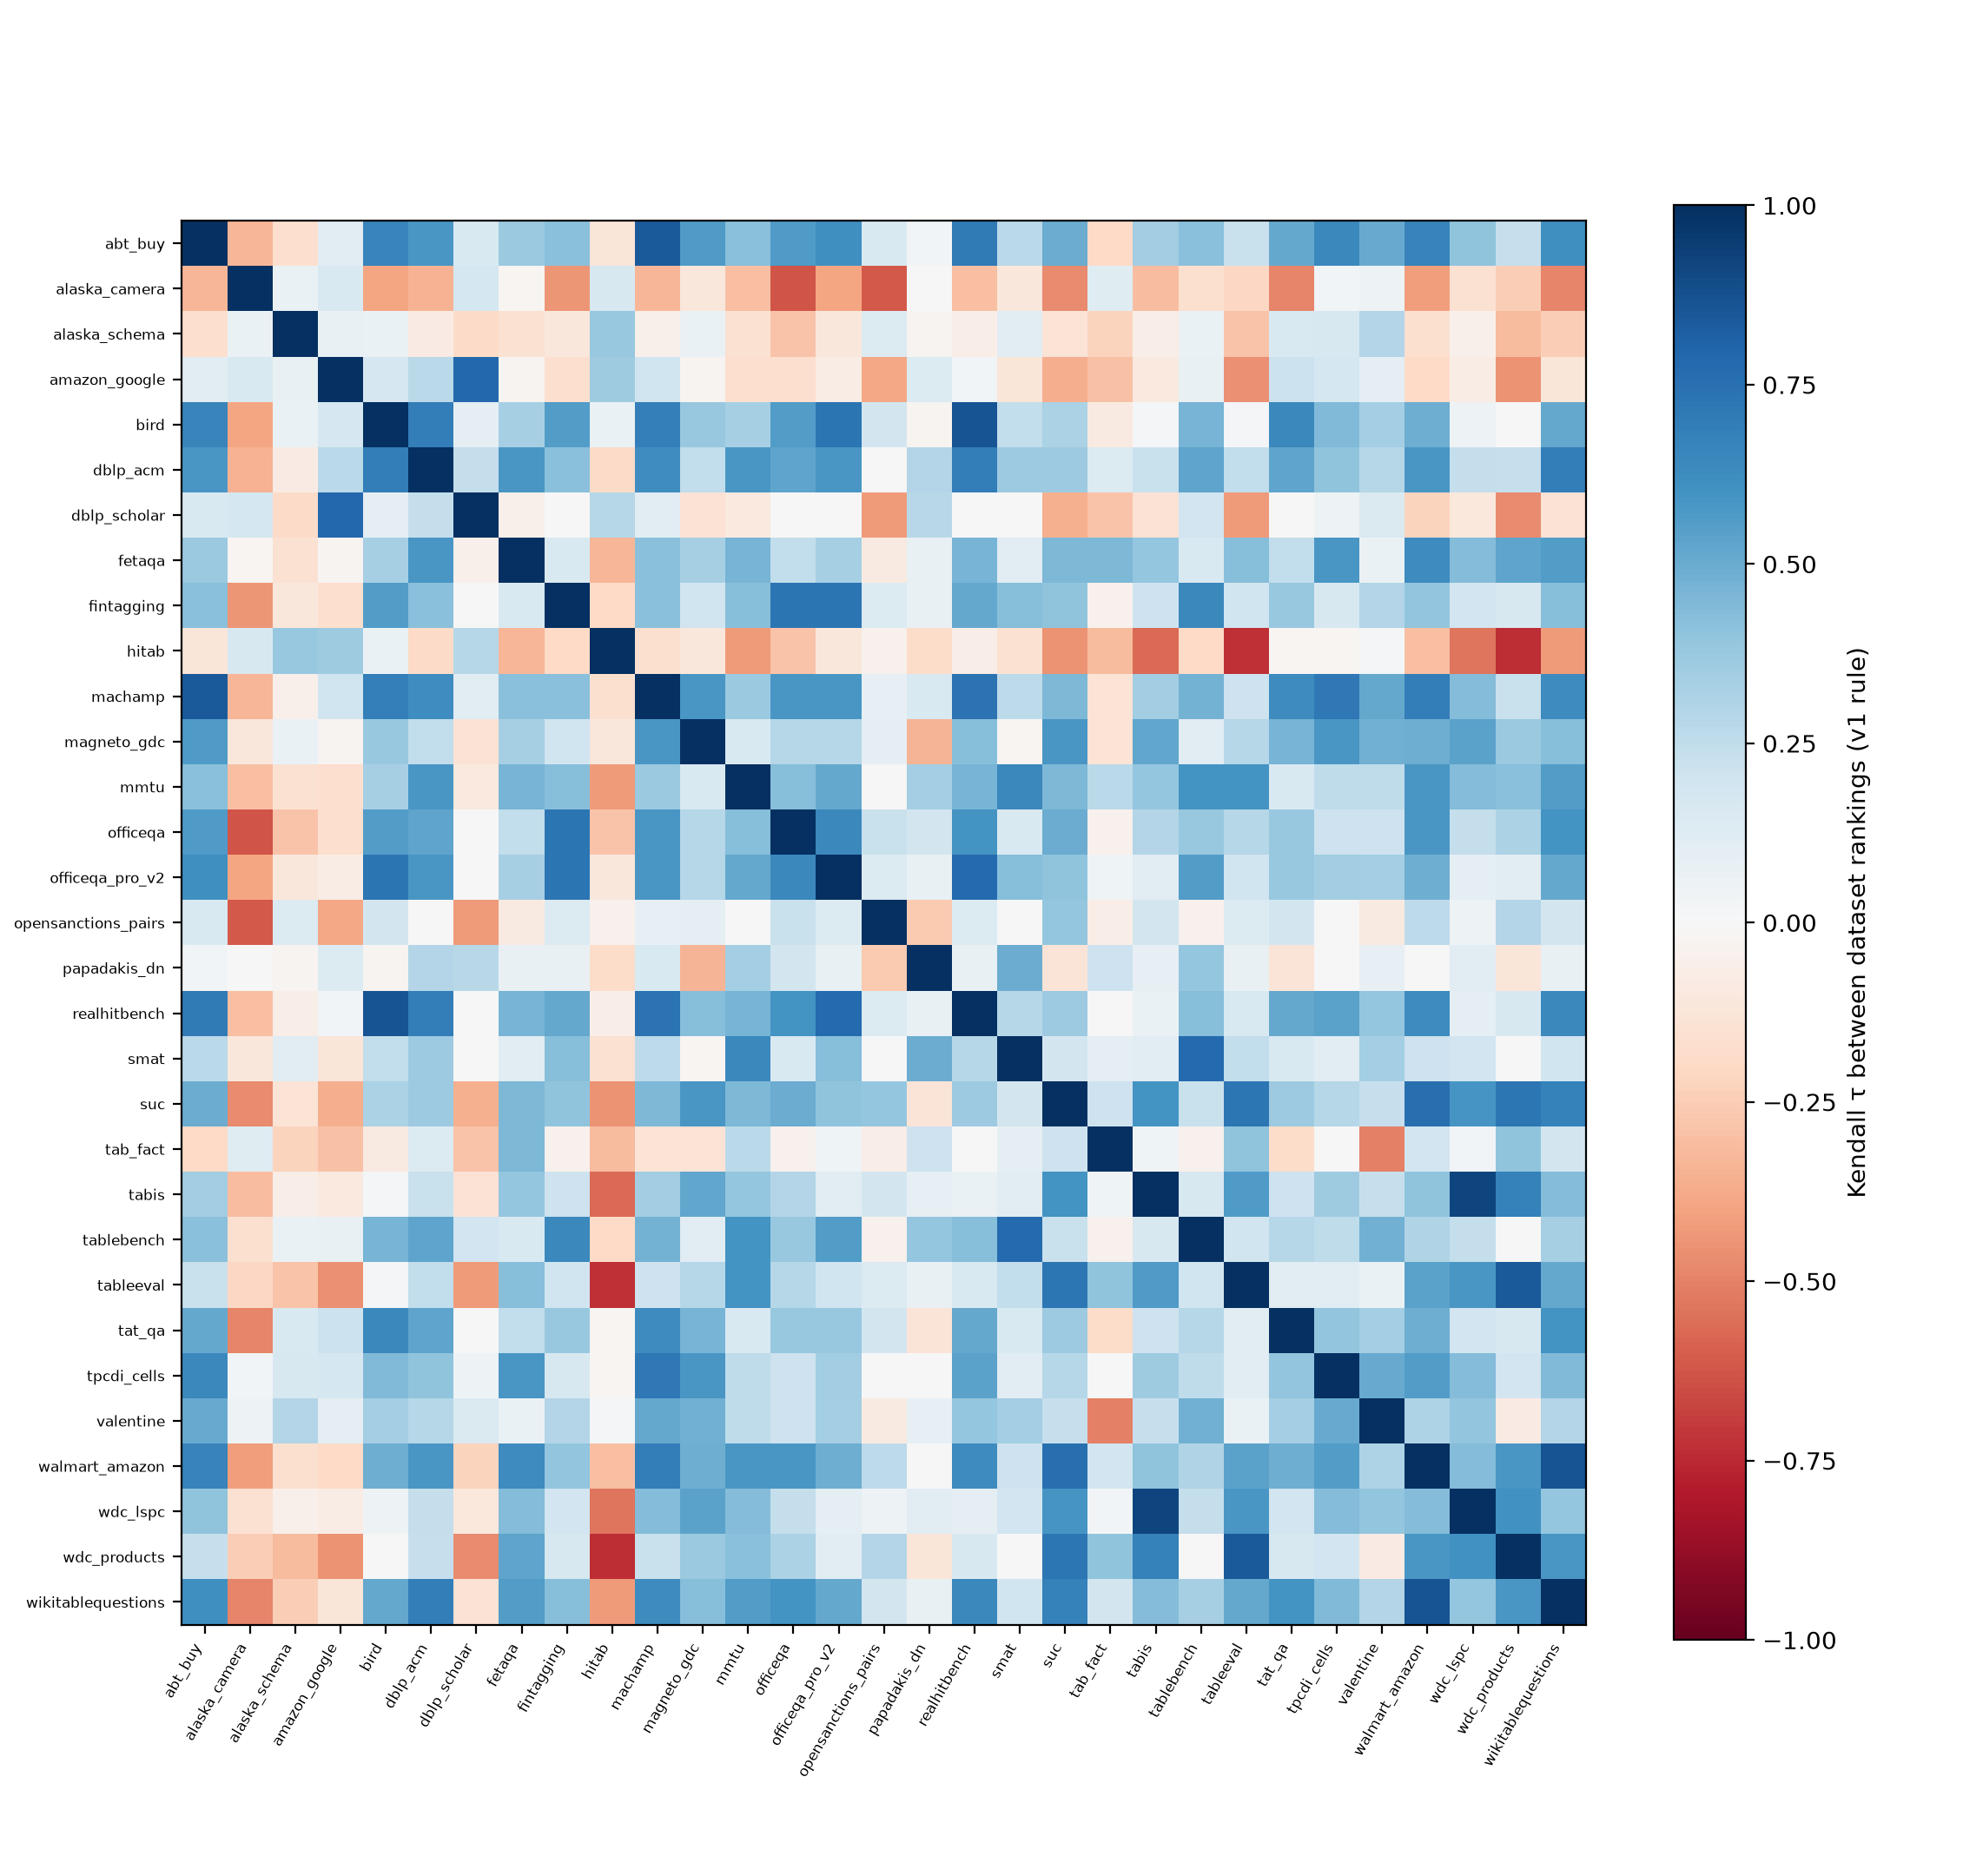
\includegraphics[width=0.9\textwidth]{fig_dataset_tau.png}\caption{Kendall $\tau$ between dataset rankings under v1.}\label{figall:fig_dataset_tau}\end{figure}
\noindent{\small \textbf{What it encodes.} Kendall $\tau$ between the model rankings of every pair of datasets under v1 (blue agreement, red disagreement). \textbf{How to read it.} Blocks of blue are groups of datasets that rank the models the same way; red rows are datasets that disagree with most others. \textbf{What it shows.} Mean pairwise $\tau$ is +0.20 and Kendall's $W$ is 0.26: datasets agree about the ends of the table and disagree about the middle. Alaska Camera and HiTab are red against most of the suite.}
\clearpage

\begin{figure}[htbp]\centering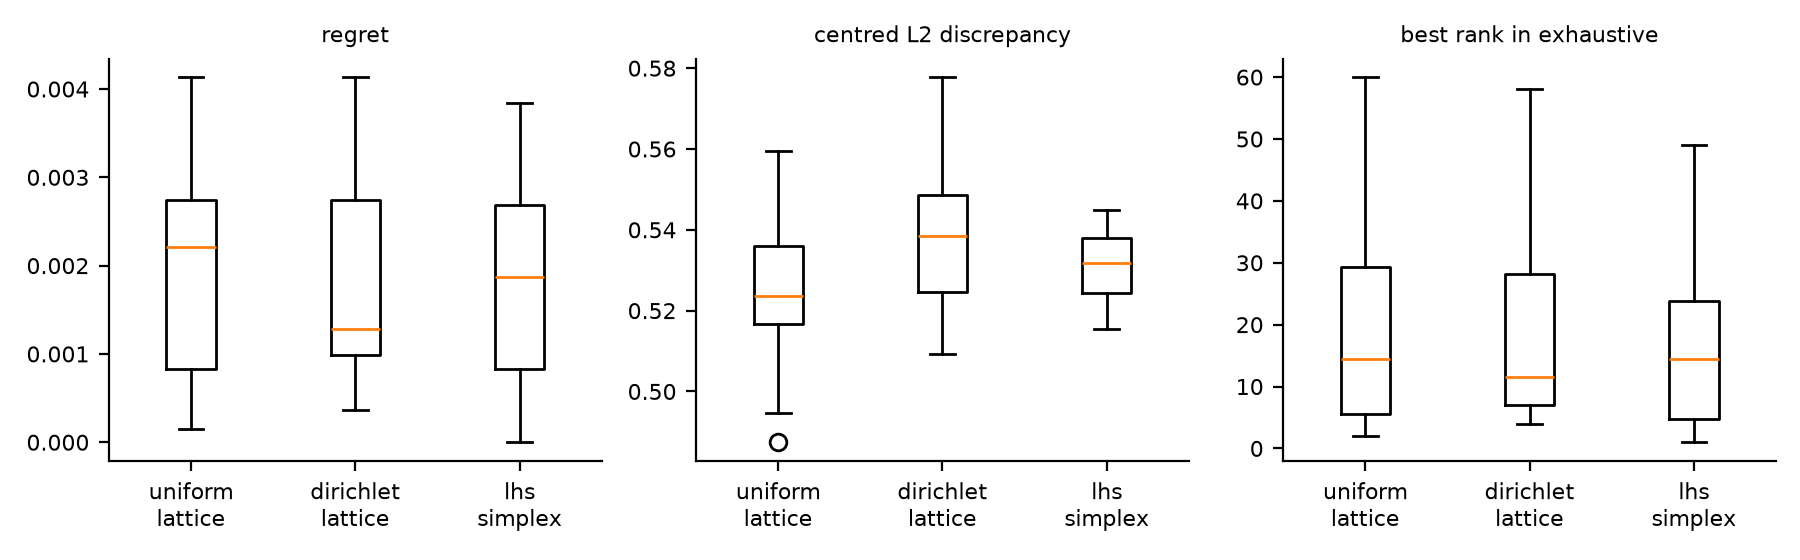
\includegraphics[width=0.9\textwidth]{fig_design_metrics.png}\caption{Sampled designs over 20 seeds: regret against the exhaustive optimum, centred $L_2$ discrepancy and rank of the found best.}\label{figall:fig_design_metrics}\end{figure}
\noindent{\small \textbf{What it encodes.} Box plots over 20 seeds of regret, centred $L_2$ discrepancy (coverage of the simplex, lower is more even) and the rank of the found best within the exhaustive grid, per design. \textbf{How to read it.} Lower discrepancy means the sample is spread more evenly; lower regret and rank mean the sample found a better point. \textbf{What it shows.} The three designs are interchangeable at this budget; the uniform lattice has marginally better coverage and the Latin hypercube marginally lower regret, and all three differ by less than the bootstrap noise of $J$.}
\clearpage

\begin{figure}[htbp]\centering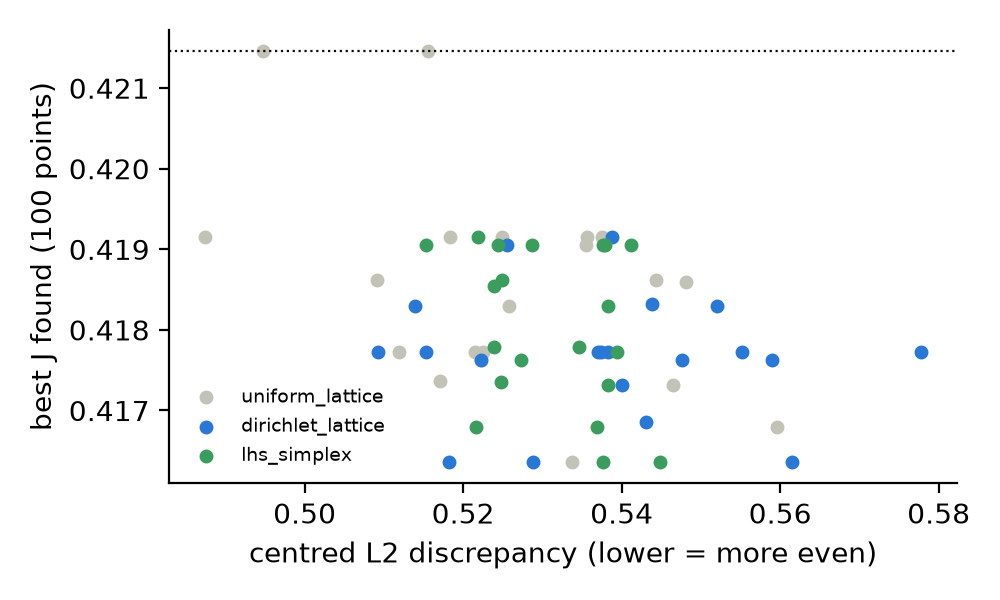
\includegraphics[width=0.9\textwidth]{fig_designs.png}\caption{Sampled designs against the exhaustive optimum.}\label{figall:fig_designs}\end{figure}
\noindent{\small \textbf{What it encodes.} For three sampling designs of 100 weightings (uniform lattice, Dirichlet-snapped, Latin hypercube) and 20 seeds each, the best $J$ found, against the exhaustive optimum. \textbf{How to read it.} Regret is the vertical distance to the exhaustive best; the spread across seeds is the risk of an unlucky sample. \textbf{What it shows.} Every design and every seed lands within 0.004 of the optimum; the worst seed of any design still finds a top-60 weighting. With four weights the exhaustive grid is free, so the designs serve only to show that sampling would have sufficed.}
\clearpage

\begin{figure}[htbp]\centering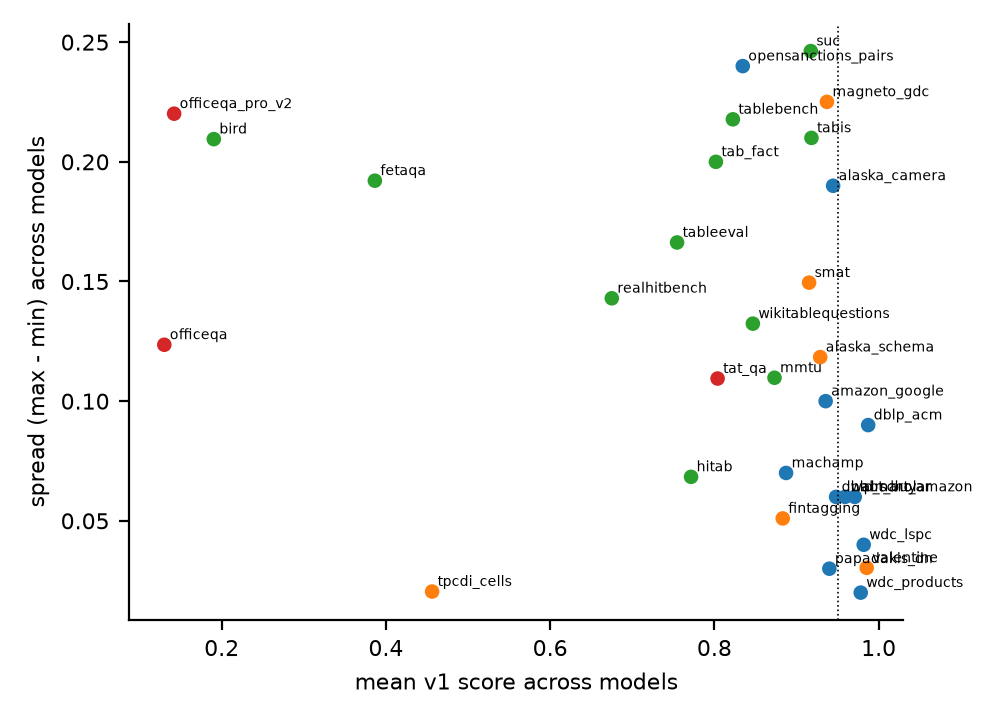
\includegraphics[width=0.9\textwidth]{fig_diagnostics_scatter.png}\caption{Dataset diagnostics: mean score against spread across models; dotted line marks the ceiling flag.}\label{figall:fig_diagnostics_scatter}\end{figure}
\noindent{\small \textbf{What it encodes.} Each dataset placed by its mean v1 score across models (horizontal) and the spread between the best and worst model (vertical); the dotted line is the ceiling flag. \textbf{How to read it.} Datasets at the right with low spread are at ceiling and cannot rank models; datasets with high spread are the discriminating ones. \textbf{What it shows.} 3 datasets are flagged at ceiling (mean $\ge$ 0.95, spread $\le$ 0.04). They remain inside the objective in this run and are listed as a limitation.}
\clearpage

\begin{figure}[htbp]\centering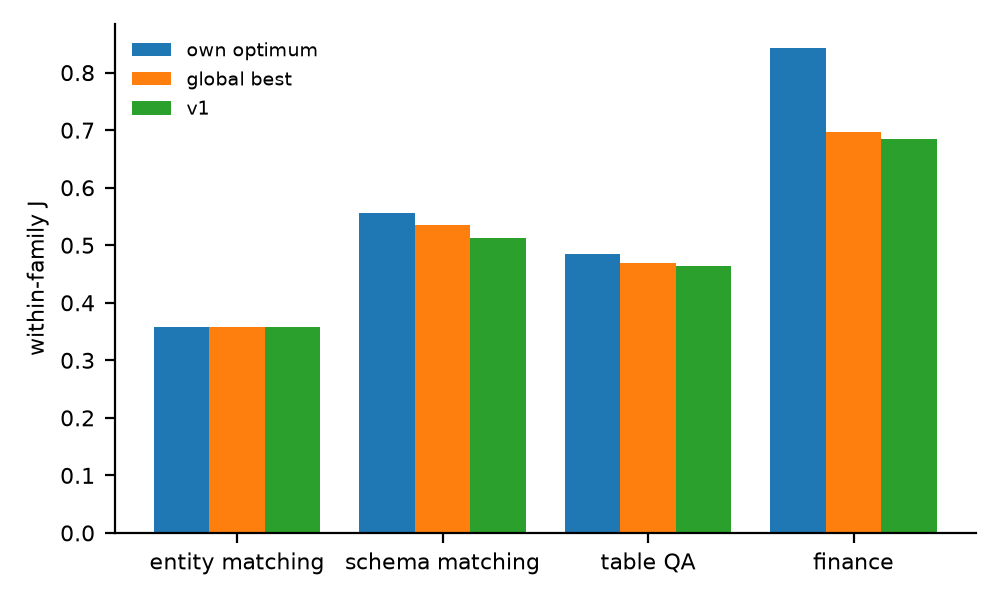
\includegraphics[width=0.9\textwidth]{fig_family_j.png}\caption{Within-family agreement $J$ under each family's own optimum, the global best and v1.}\label{figall:fig_family_j}\end{figure}
\noindent{\small \textbf{What it encodes.} Within-family agreement $J$ (computed over that family's datasets only) under the family's own optimum, the global best and v1. \textbf{How to read it.} The gap between the first bar and the other two is what family-specific weights would gain for that family. \textbf{What it shows.} Within a family the datasets agree far more than across the suite (finance highest, entity matching lowest), and the family optimum beats the global best by a visible margin only for table QA and finance.}
\clearpage

\begin{figure}[htbp]\centering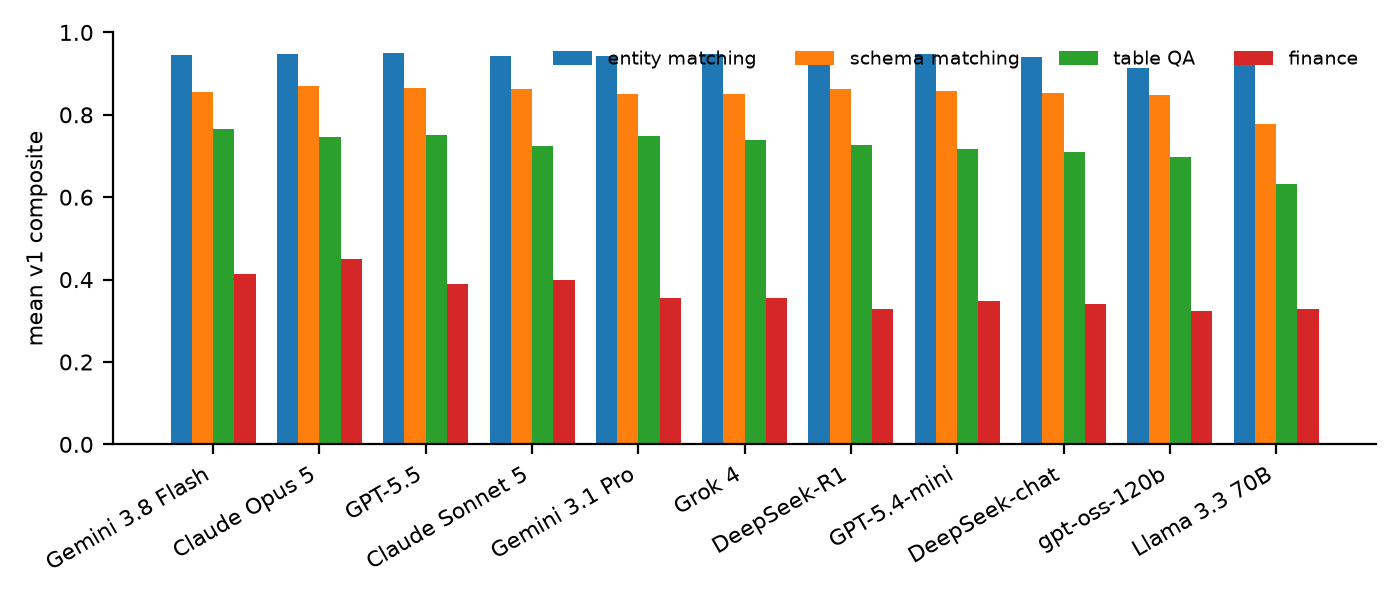
\includegraphics[width=0.9\textwidth]{fig_family_scores.png}\caption{Mean v1 composite per model within each task family.}\label{figall:fig_family_scores}\end{figure}
\noindent{\small \textbf{What it encodes.} For each model, four bars: its mean v1 composite within entity matching, schema matching, table QA and finance. \textbf{How to read it.} Compare bars of the same colour across models to see the family-specific ranking; compare the four bars of one model to see which family drives its overall mean. \textbf{What it shows.} Entity matching is near ceiling for every model, finance is near floor for every model, and the differences between models live in table QA and schema matching. A model's overall position is therefore decided by a minority of the suite.}
\clearpage

\begin{figure}[htbp]\centering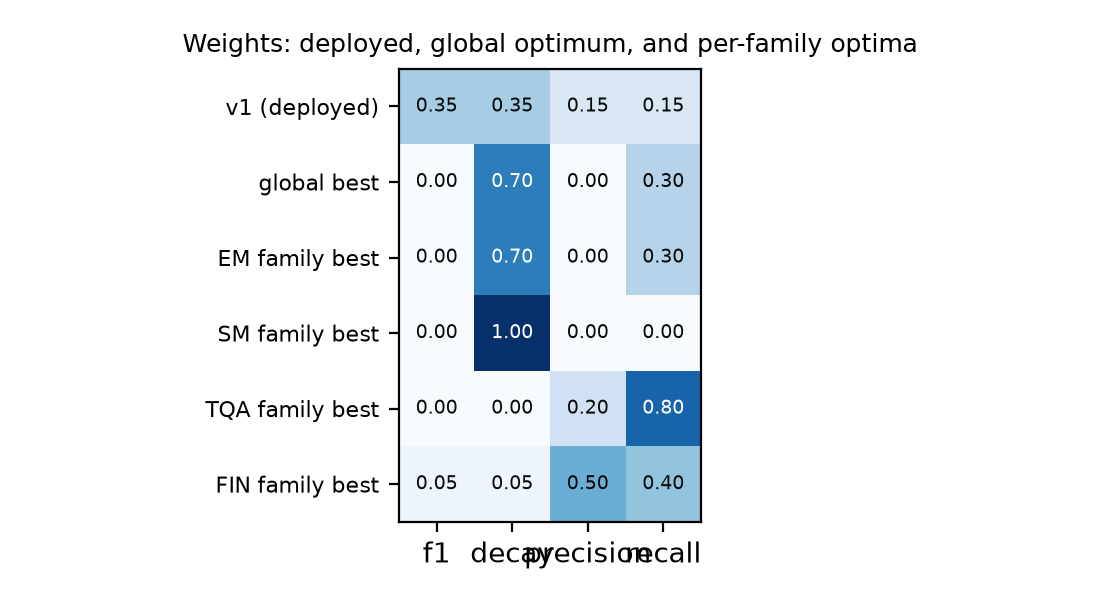
\includegraphics[width=0.9\textwidth]{fig_family_weights.png}\caption{Deployed, global-optimum and per-family weights.}\label{figall:fig_family_weights}\end{figure}
\noindent{\small \textbf{What it encodes.} The four weights of v1, of the global optimum, and of the optimum fitted inside each task family. \textbf{How to read it.} Compare the family profiles with each other and with the global point. Agreement would show the same shape in every row. \textbf{What it shows.} The families disagree: decay dominates for schema matching, recall for table QA, precision for finance. The suite-level flatness is partly these pulls cancelling, which also explains why leave-one-family-out re-fits land far from the global best.}
\clearpage

\begin{figure}[htbp]\centering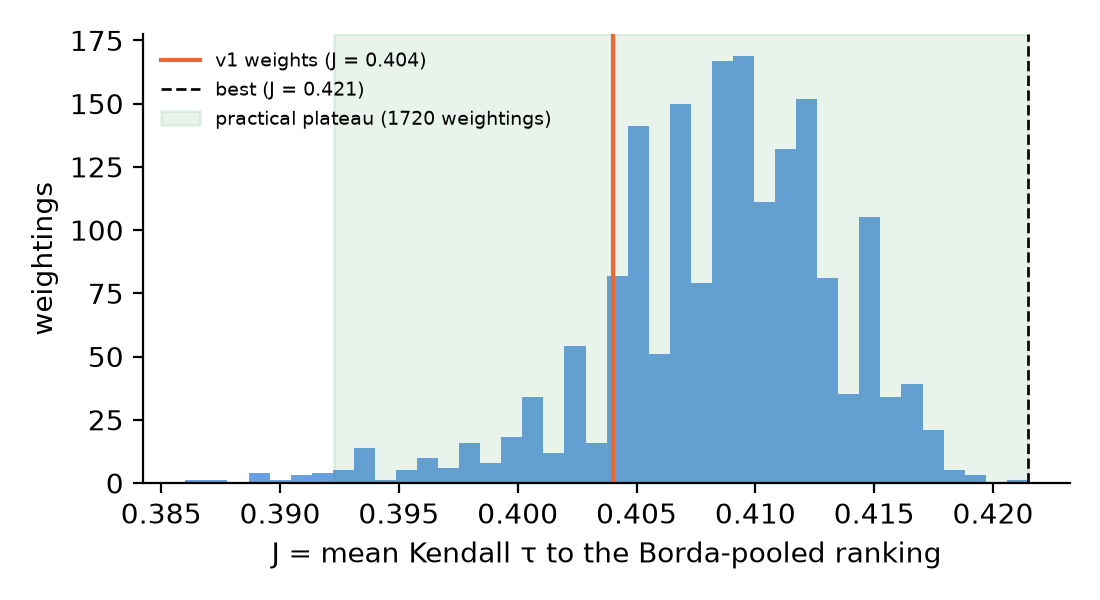
\includegraphics[width=0.9\textwidth]{fig_j_histogram.png}\caption{Distribution of $J$ over the 1,771 weightings with v1, the best and the plateau band.}\label{figall:fig_j_histogram}\end{figure}
\noindent{\small \textbf{What it encodes.} The horizontal axis is the agreement objective $J$ (mean Kendall $\tau$ between each dataset's model ranking and the Borda-pooled ranking); the bars count how many of the 1,771 step-0.05 weightings fall in each bin. The vertical lines mark the deployed weights (v1) and the best weighting; the shaded band is the plateau of weightings statistically indistinguishable from the best. \textbf{How to read it.} If the weights mattered, the histogram would be wide and v1 would sit in a low tail far from the best. Instead the whole distribution spans 0.376--0.414, v1 sits at 0.398 and the best at 0.414, and the plateau covers 1,749 of 1,771 points. \textbf{What it shows.} The objective is flat: moving weight between F1, decay, precision and recall changes $J$ by less than the bootstrap noise of a single point, so no weighting is distinguishable from v1 on this suite.}
\clearpage

\begin{figure}[htbp]\centering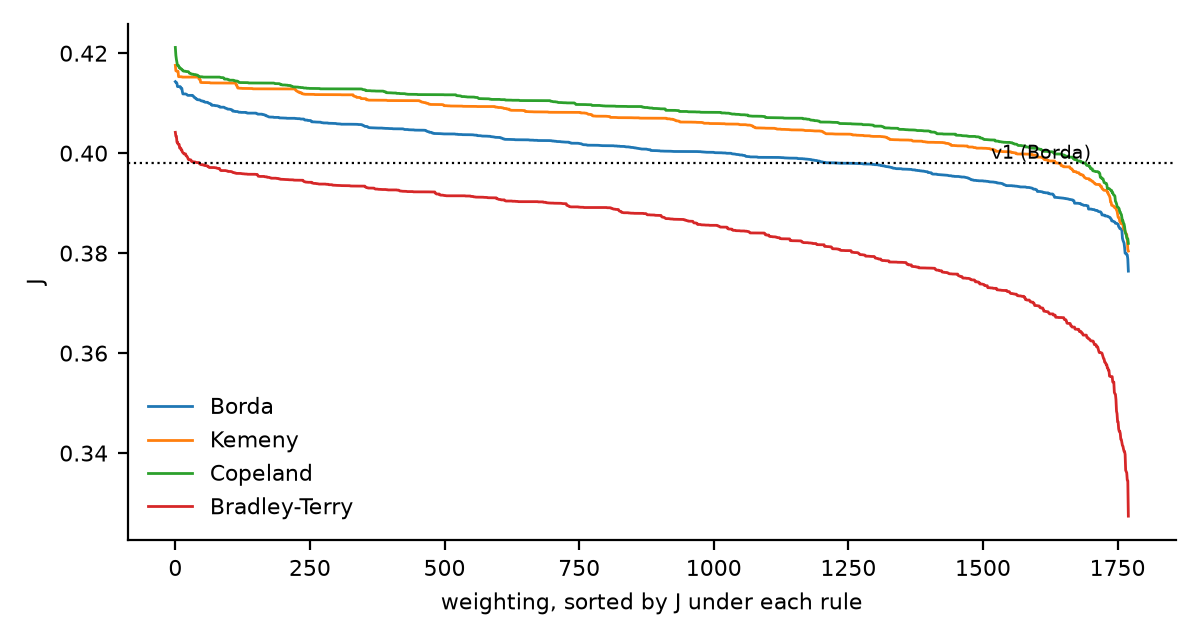
\includegraphics[width=0.9\textwidth]{fig_j_pooling_rules.png}\caption{Agreement objective $J$ over all 1,771 weightings under four pooling rules (each curve sorted separately). The landscape is flat under every rule.}\label{figall:fig_j_pooling_rules}\end{figure}
\noindent{\small \textbf{What it encodes.} The objective recomputed under four ways of pooling the 31 per-dataset rankings into one (Borda, Kemeny, Copeland, Bradley--Terry), each curve sorted separately from best to worst. \textbf{How to read it.} The curves answer whether the flatness is an artefact of Borda pooling. If another rule produced a steeper curve or a clear winner, the choice of pooling rule would matter for the audit. \textbf{What it shows.} All four curves are flat and sit within a few hundredths of each other; which weighting is ``best'' changes with the rule (v1's rank moves from 1,116 under Bradley--Terry to 1,311 under Kemeny), confirming that rank inside the lattice is noise.}
\clearpage

\begin{figure}[htbp]\centering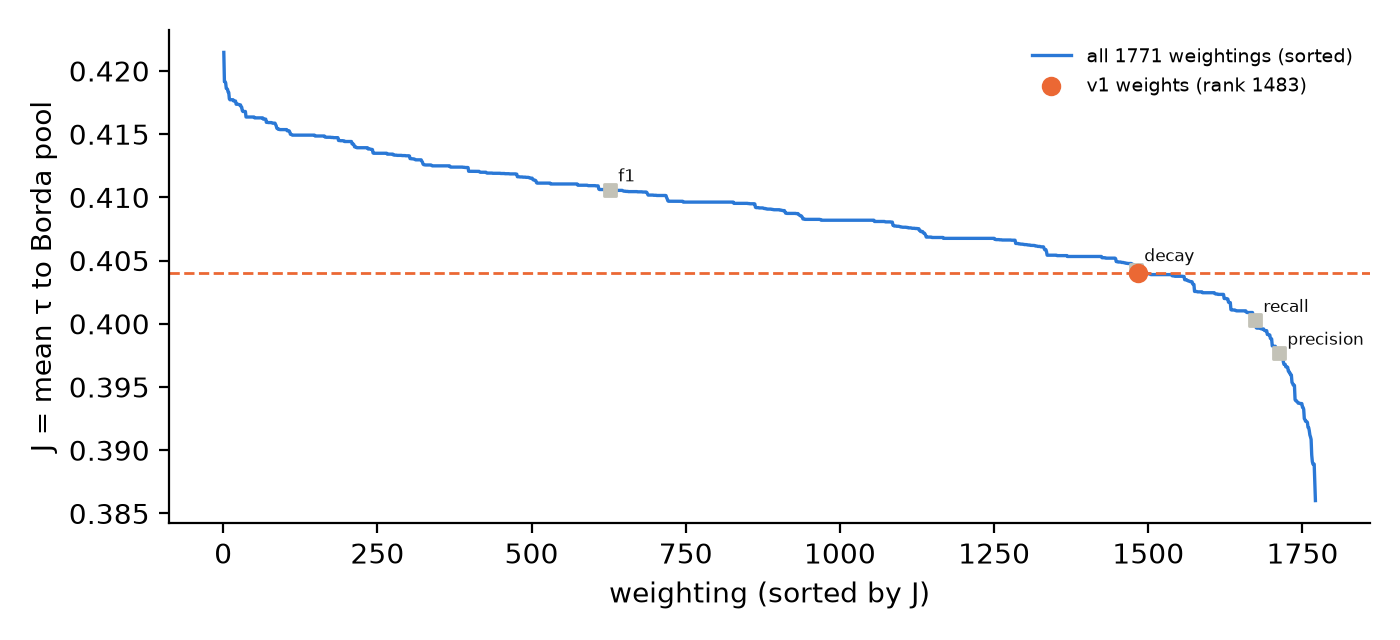
\includegraphics[width=0.9\textwidth]{fig_landscape.png}\caption{Sorted $J$ with v1 and the four single-ingredient corners.}\label{figall:fig_landscape}\end{figure}
\noindent{\small \textbf{What it encodes.} Every weighting sorted from best (left) to worst (right) by $J$; the curve is $J$ itself, and the marked points are v1 and the four single-ingredient corners (F1 only, decay only, precision only, recall only). \textbf{How to read it.} The height of the curve at any rank is the $J$ of that weighting; the vertical drop from left to right is the whole range the search could ever exploit. A rank far to the right looks bad until the vertical scale is read: v1 is at rank 1,260 of 1,771, but the curve drops only 0.038 from first to last. \textbf{What it shows.} The curve is nearly horizontal until the last few dozen weightings, which are the extreme corners. Rank inside such a curve carries no information, which is why the report quotes the plateau and the out-of-bag difference instead of v1's rank.}
\clearpage

\begin{figure}[htbp]\centering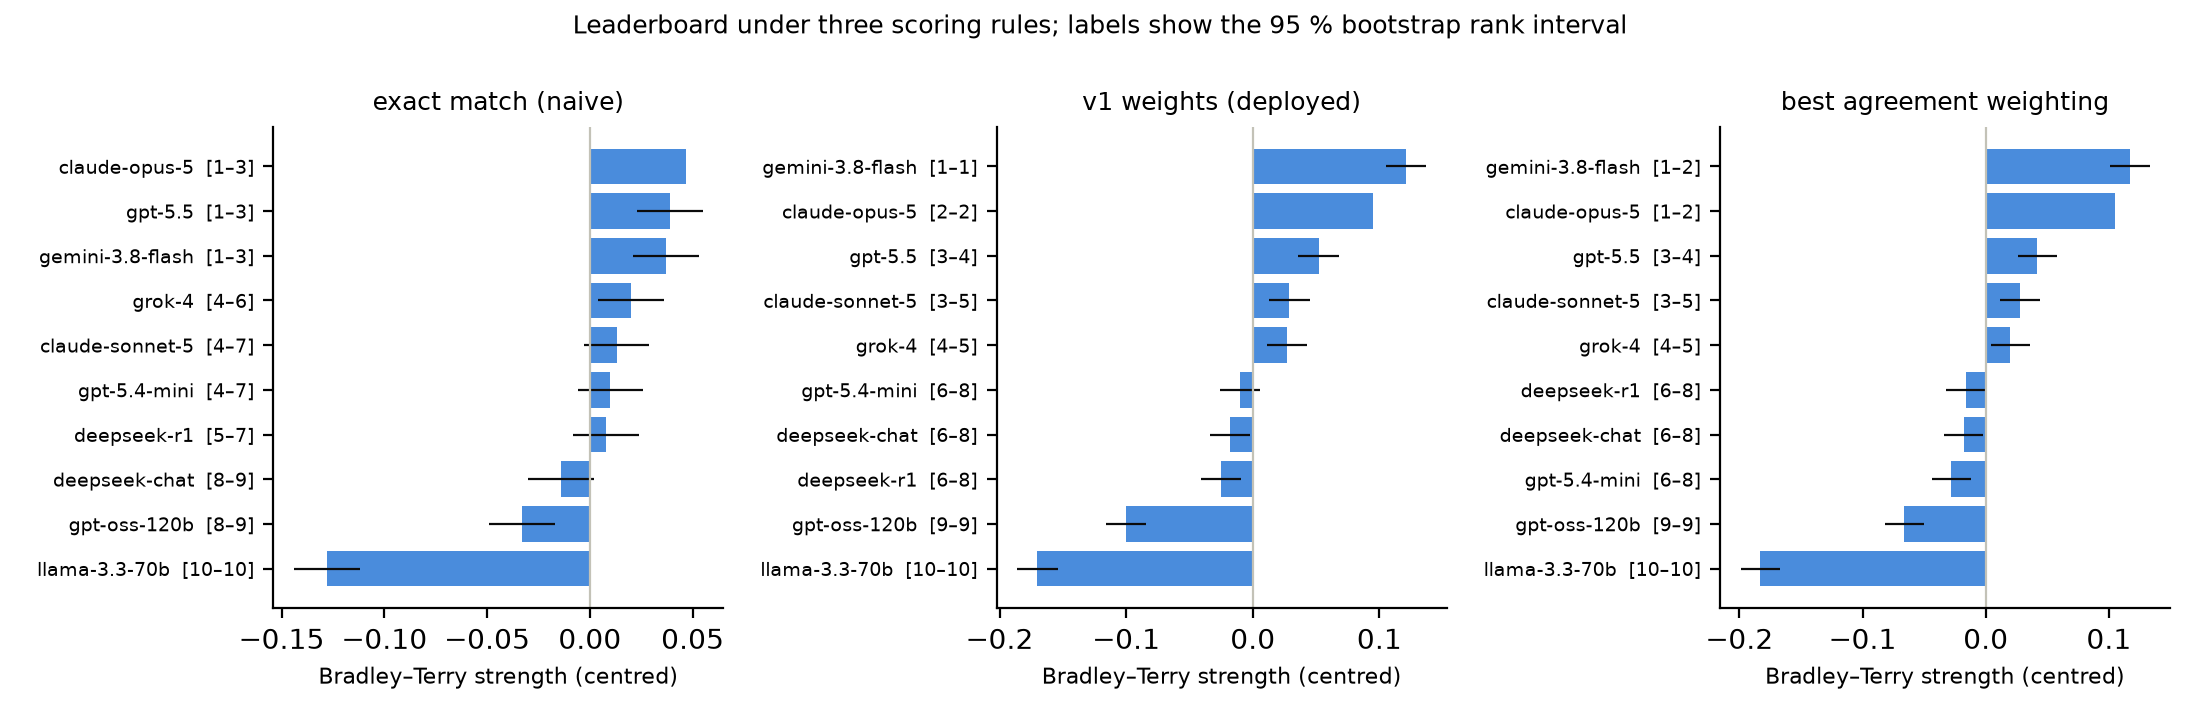
\includegraphics[width=0.9\textwidth]{fig_leaderboard_rules.png}\caption{Bradley--Terry strengths with rank intervals under exact match, v1 and the best-$J$ weighting.}\label{figall:fig_leaderboard_rules}\end{figure}
\noindent{\small \textbf{What it encodes.} Bradley--Terry strengths (log-odds of winning an item against the reference model, with standard errors) and bootstrap rank intervals under exact match, v1 and the best-$J$ weighting. \textbf{How to read it.} Overlapping intervals mean the order is not established; a model whose point moves between panels is one whose position depends on the scoring rule. \textbf{What it shows.} The ends are fixed under every rule (Llama 3.3 70B last, gpt-oss-120b ninth); the top three (Gemini 3.8 Flash, Claude Opus 5, GPT-5.5) reorder with the rule. Exact match favours Opus; the graded rules favour Gemini Flash.}
\clearpage

\begin{figure}[htbp]\centering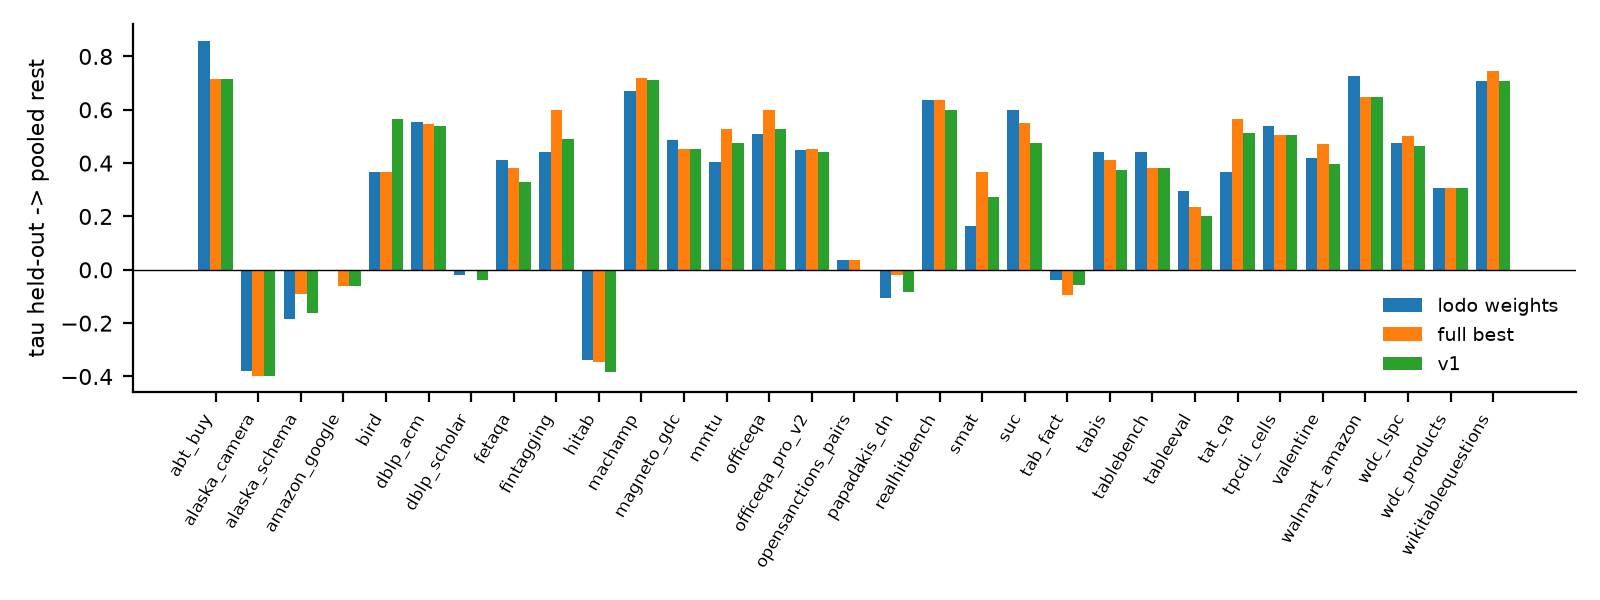
\includegraphics[width=0.9\textwidth]{fig_lodo_tau.png}\caption{Leave-one-dataset-out: agreement of the held-out dataset with the pooled ranking of the rest, under weights fitted without it, the full-data best and v1.}\label{figall:fig_lodo_tau}\end{figure}
\noindent{\small \textbf{What it encodes.} For each dataset held out in turn: the Kendall $\tau$ between its model ranking and the pooled ranking of the other 30, under weights re-fitted without it, the full-data best, and v1. \textbf{How to read it.} If weight search generalised, the re-fitted bars would beat v1's on most datasets. Negative bars are datasets whose ranking opposes the consensus however the weights are set. \textbf{What it shows.} Means are +0.33 (re-fitted), +0.35 (full best) and +0.32 (v1); re-fitting helps on 20 datasets and hurts on 9. The same handful of sets (Alaska Camera, HiTab, Alaska schema) are negative under every rule.}
\clearpage

\begin{figure}[htbp]\centering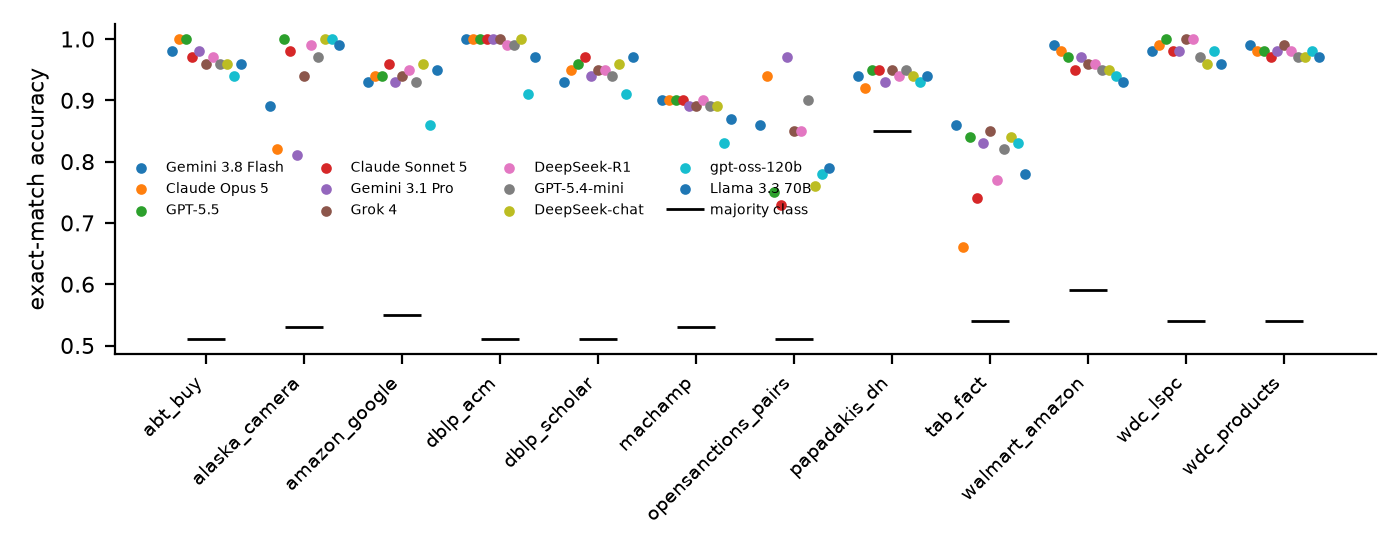
\includegraphics[width=0.9\textwidth]{fig_majority_baselines.png}\caption{Exact-match accuracy of every model on the boolean datasets against the majority-class baseline of each pool.}\label{figall:fig_majority_baselines}\end{figure}
\noindent{\small \textbf{What it encodes.} For the boolean datasets, every model's exact-match accuracy against the majority-class baseline of the pool (the accuracy of always answering the more common label). \textbf{How to read it.} A model below the baseline line is doing worse than a constant answer on that dataset. \textbf{What it shows.} Every model clears the baseline on every boolean set, usually by a wide margin; the balanced pools make the baseline about 0.5 so this is a weak test, which is why the official-ratio F1 is reported beside it.}
\clearpage

\begin{figure}[htbp]\centering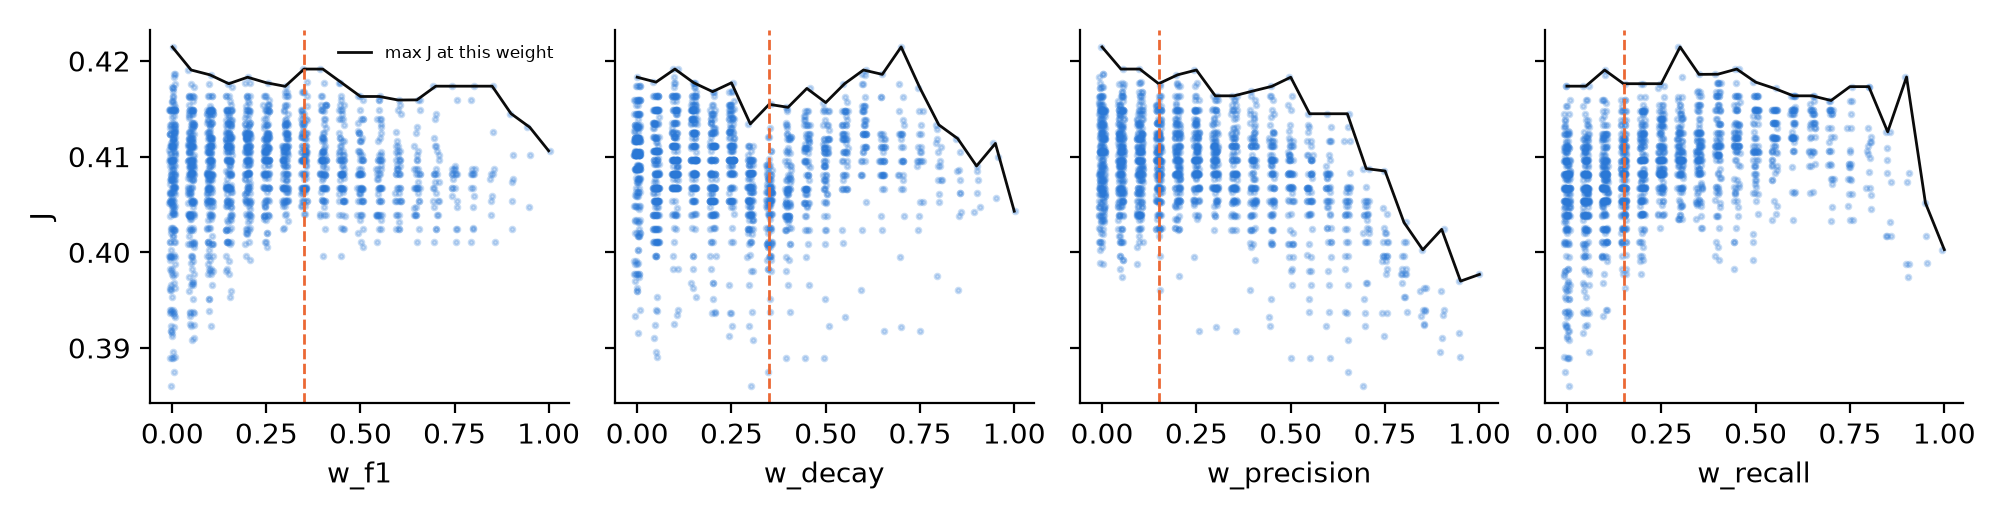
\includegraphics[width=0.9\textwidth]{fig_marginals.png}\caption{$J$ against each of the four weights.}\label{figall:fig_marginals}\end{figure}
\noindent{\small \textbf{What it encodes.} Four panels, one per ingredient; each point is one weighting placed by the weight it gives that ingredient (horizontal) and its $J$ (vertical); the line is the mean $J$ at each weight level. \textbf{How to read it.} A sloping mean line would say that more (or less) of that ingredient helps; a flat line says the ingredient's weight is irrelevant. The vertical scatter at each level is the effect of the other three weights. \textbf{What it shows.} The mean lines drift by at most 0.017 of $J$ across the whole range (precision is the steepest, falling as its weight approaches 1); no ingredient has a slope worth acting on, and the scatter around each line is larger than any slope.}
\clearpage

\begin{figure}[htbp]\centering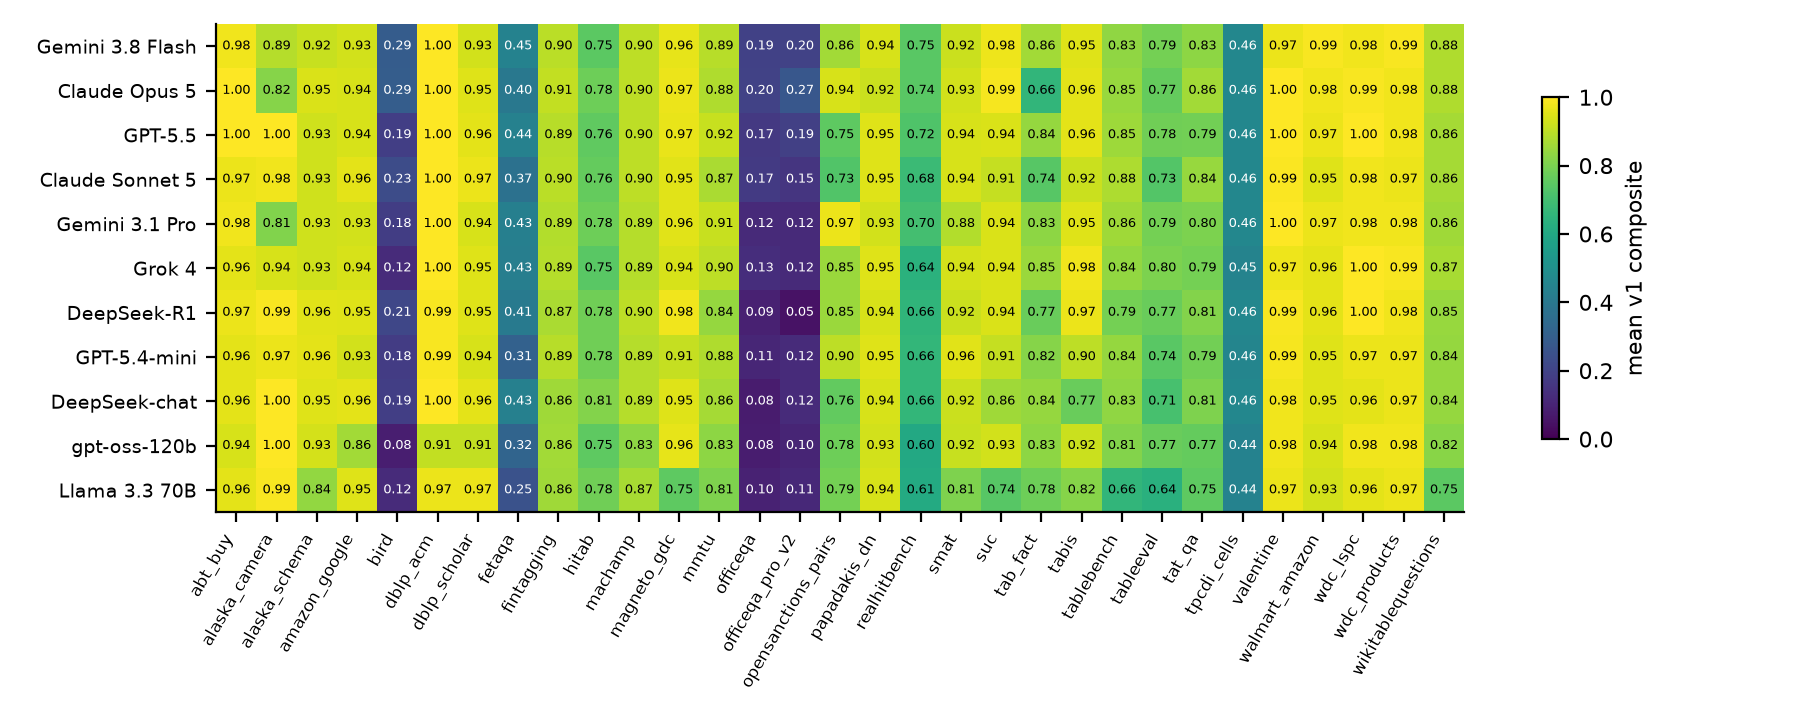
\includegraphics[width=0.9\textwidth]{fig_model_dataset_heatmap.png}\caption{Mean v1 composite score per model and dataset (models in Bradley--Terry order under v1).}\label{figall:fig_model_dataset_heatmap}\end{figure}
\noindent{\small \textbf{What it encodes.} Rows are the ten models in Bradley--Terry order under v1; columns are the 31 datasets; each cell is the model's mean v1 composite on that dataset (dark = high). \textbf{How to read it.} Columns show how hard a dataset is for everyone (BIRD and the two OfficeQA sets are dark for all models); rows show a model's profile. A leaderboard is a summary of this matrix, so any disagreement between datasets is visible here as a row that is high in one column and low in another. \textbf{What it shows.} Most columns are near ceiling with tiny spreads (the matching sets); the spread that separates models comes from a dozen table and document sets. No row dominates every column.}
\clearpage

\begin{figure}[htbp]\centering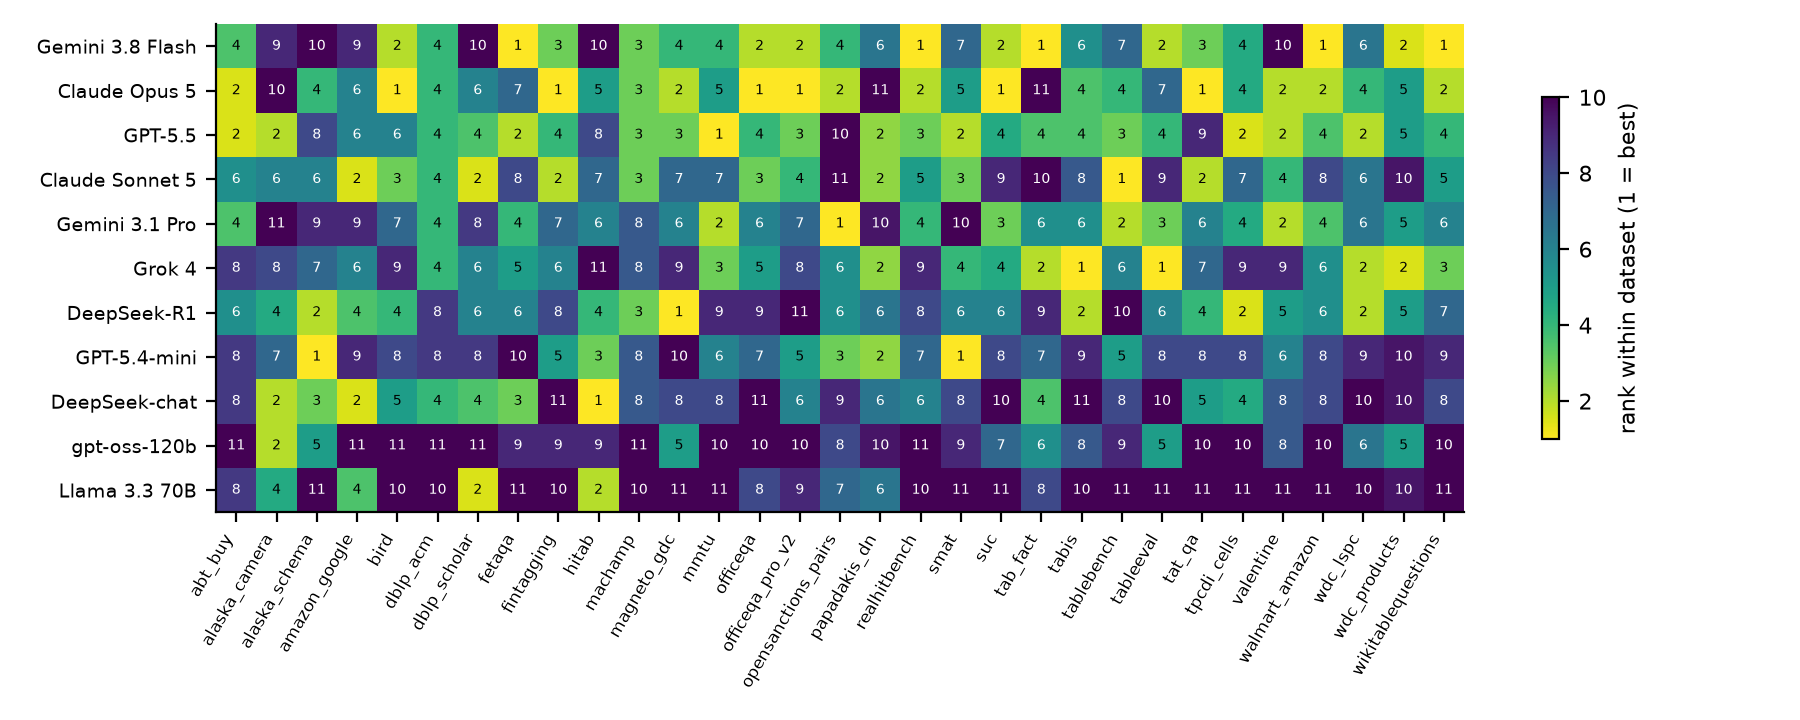
\includegraphics[width=0.9\textwidth]{fig_model_dataset_ranks.png}\caption{Rank of each model inside each dataset under v1 (ties by average rank).}\label{figall:fig_model_dataset_ranks}\end{figure}
\noindent{\small \textbf{What it encodes.} The same matrix as the score heatmap, but each column is replaced by the within-dataset rank (1 = best, ties averaged). \textbf{How to read it.} A perfectly consistent suite would show each row as a single colour. Colour changes along a row are datasets that rank that model differently from the rest. \textbf{What it shows.} Only the bottom rows are nearly uniform; the top three rows trade first place from column to column (no model is first on more than 6 datasets), which is the picture behind Kendall's $W$ of 0.26 among datasets.}
\clearpage

\begin{figure}[htbp]\centering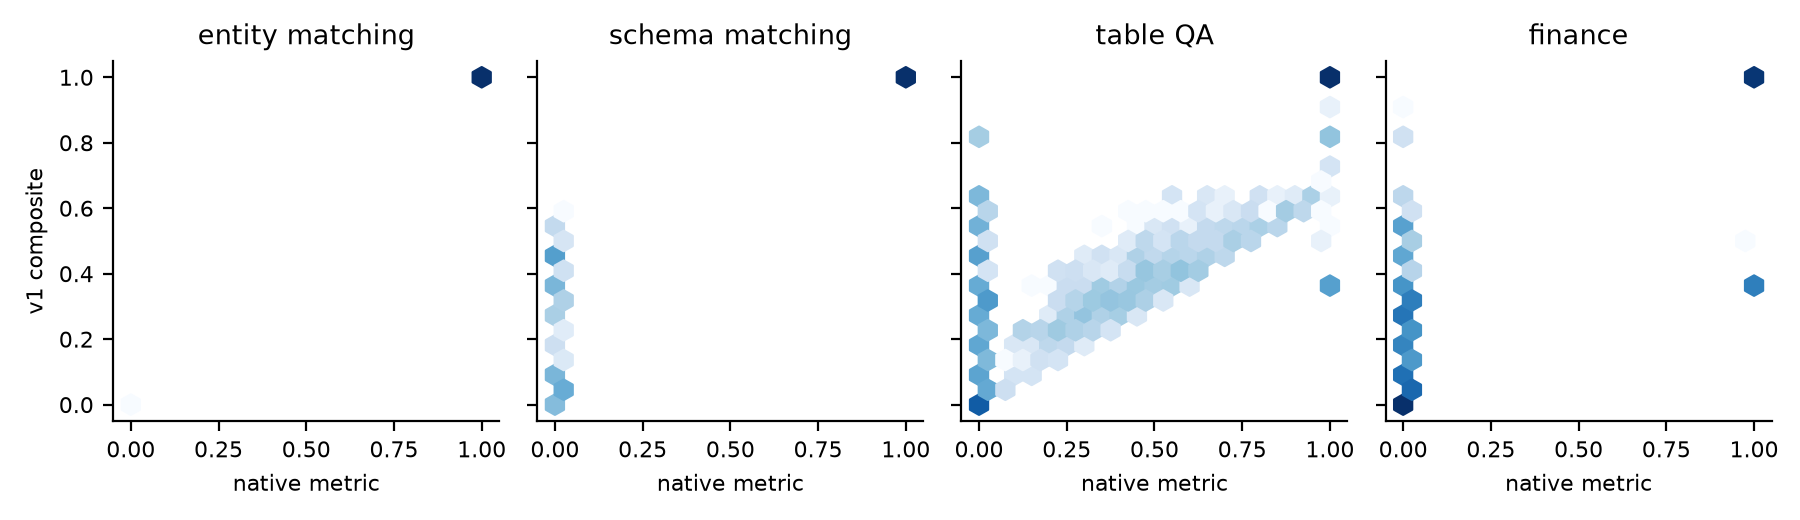
\includegraphics[width=0.9\textwidth]{fig_native_vs_composite.png}\caption{Per-answer native metric against the v1 composite, by family (log-count hexbins).}\label{figall:fig_native_vs_composite}\end{figure}
\noindent{\small \textbf{What it encodes.} One panel per family; each answer placed by its dataset's native metric (horizontal) and its v1 composite (vertical), with cell colour showing how many answers fall there (log scale). \textbf{How to read it.} Mass on the diagonal means the composite agrees with the native metric; mass off the diagonal is where the four ingredients give partial credit (above) or penalise (below) relative to the dataset's own rule. \textbf{What it shows.} Entity and schema matching sit almost entirely on the diagonal corners (0,0) and (1,1): the composite is exact match there. Table QA and finance show the off-diagonal cloud of partial credit, which is the only place the weights can act.}
\clearpage

\begin{figure}[htbp]\centering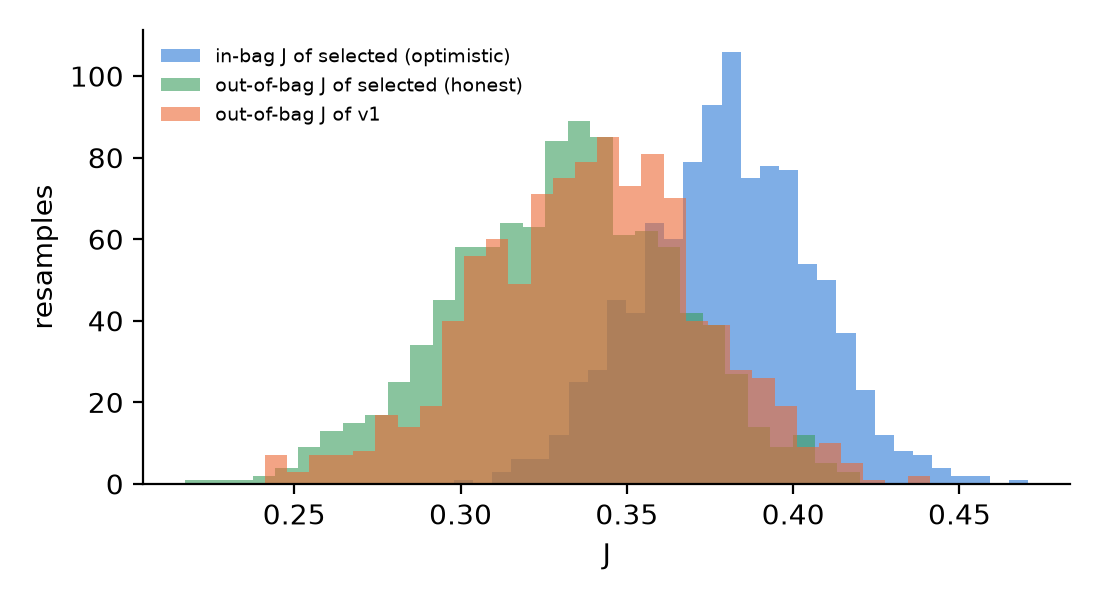
\includegraphics[width=0.9\textwidth]{fig_nested.png}\caption{In-bag vs out-of-bag $J$ of the selected weighting against v1.}\label{figall:fig_nested}\end{figure}
\noindent{\small \textbf{What it encodes.} From 1,000 item bootstraps: the in-bag $J$ of the weighting selected as best on the in-bag items, the same weighting's out-of-bag $J$, and v1's out-of-bag $J$. \textbf{How to read it.} The gap between the first two is the optimism of selection (the winner's curse); the comparison between the second and the third is the honest test of whether searching found anything. \textbf{What it shows.} The selected weighting looks 0.047 better in-bag than out of bag, and out of bag it is -0.007 from v1 with a 95\,\% interval of [-0.033, +0.011]. Searching the weights buys nothing that survives held-out items.}
\clearpage

\begin{figure}[htbp]\centering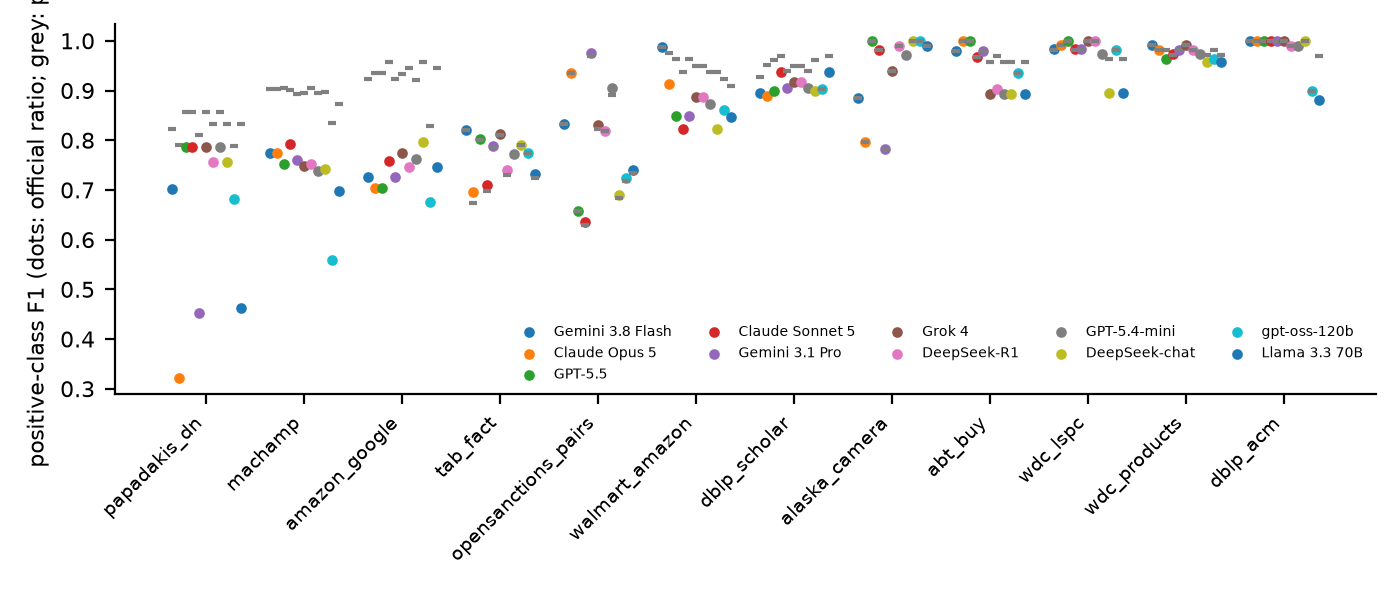
\includegraphics[width=0.9\textwidth]{fig_official_f1_models.png}\caption{Positive-class F1 on the balanced pool (grey) and at the official match ratio (coloured) per model and matching dataset.}\label{figall:fig_official_f1_models}\end{figure}
\noindent{\small \textbf{What it encodes.} For each matching dataset and model, positive-class F1 on the balanced pool (grey ticks) and at the official match ratio (coloured dots). \textbf{How to read it.} The vertical gap between tick and dot for a model is how much its balanced-pool F1 overstates its official-ratio F1; the spread of dots is the between-model difference that survives re-weighting. \textbf{What it shows.} The gap is large and similar for all models on Amazon--Google, Machamp and Papadakis--Christen, and negligible on the dense sets. Model order is mostly preserved; the absolute numbers are not.}
\clearpage

\begin{figure}[htbp]\centering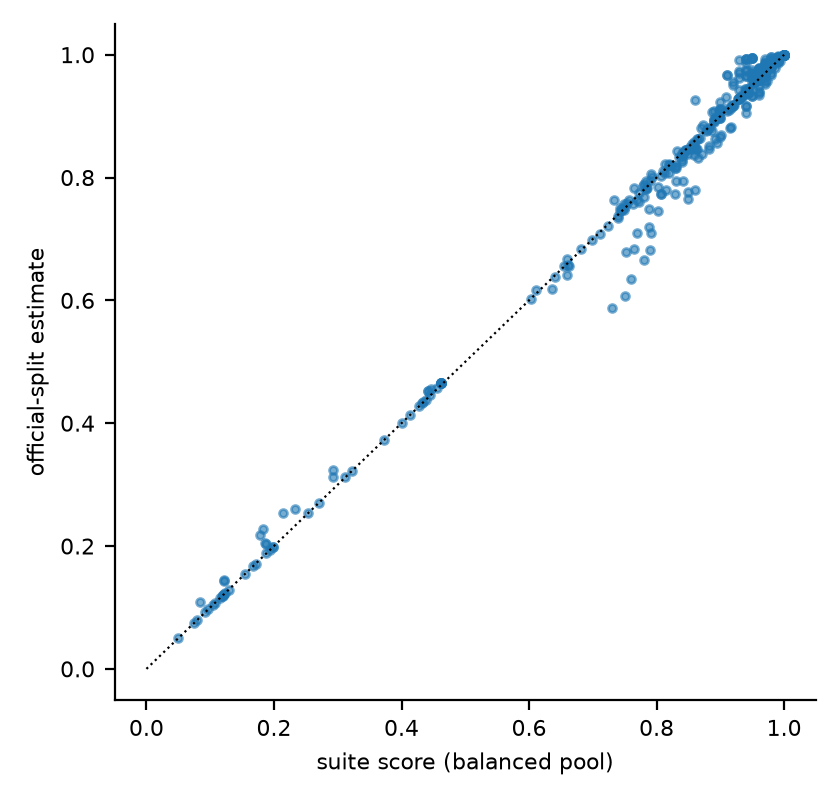
\includegraphics[width=0.9\textwidth]{fig_official_scatter.png}\caption{Suite score against post-stratified official-split estimate for every (dataset, model) pair under v1.}\label{figall:fig_official_scatter}\end{figure}
\noindent{\small \textbf{What it encodes.} Every (dataset, model) pair placed by its suite score and its post-stratified official estimate under v1. \textbf{How to read it.} Distance from the diagonal is the effect of re-weighting for that cell; the cloud's tightness is how comparable the suite numbers are to published ones. \textbf{What it shows.} Almost every cell is within a few hundredths of the diagonal; the exceptions are the sparse matching sets and OpenSanctions, where the official class ratio differs most from 50/50.}
\clearpage

\begin{figure}[htbp]\centering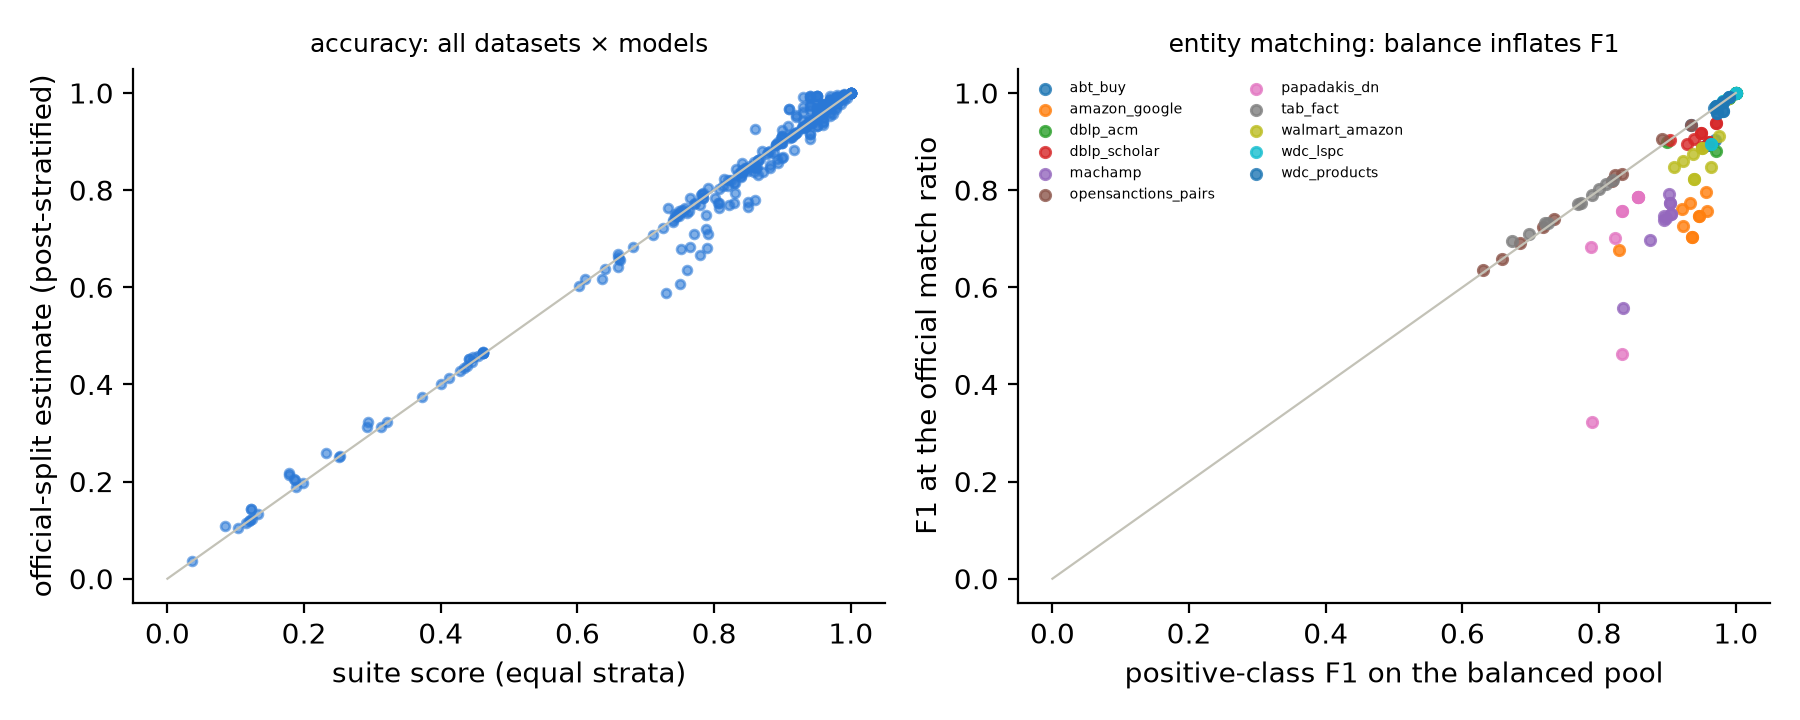
\includegraphics[width=0.9\textwidth]{fig_official_split.png}\caption{Suite score vs post-stratified official estimate; matching F1 at the official ratio.}\label{figall:fig_official_split}\end{figure}
\noindent{\small \textbf{What it encodes.} Per dataset, the suite score (mean over the balanced, stratified pool) against the same answers re-weighted to the official split's stratum or class proportions; for the matching sets, positive-class F1 on the pool against F1 at the official match ratio. \textbf{How to read it.} Points on the diagonal are datasets whose pool already matches the official split; points below it are where the balanced pool overstates performance. \textbf{What it shows.} Accuracy moves by at most 0.09; F1 on the matching sets drops by up to 0.19 where matches are rare, through precision: at a 2\,\% match rate a 1\,\% false-positive rate halves precision.}
\clearpage

\begin{figure}[htbp]\centering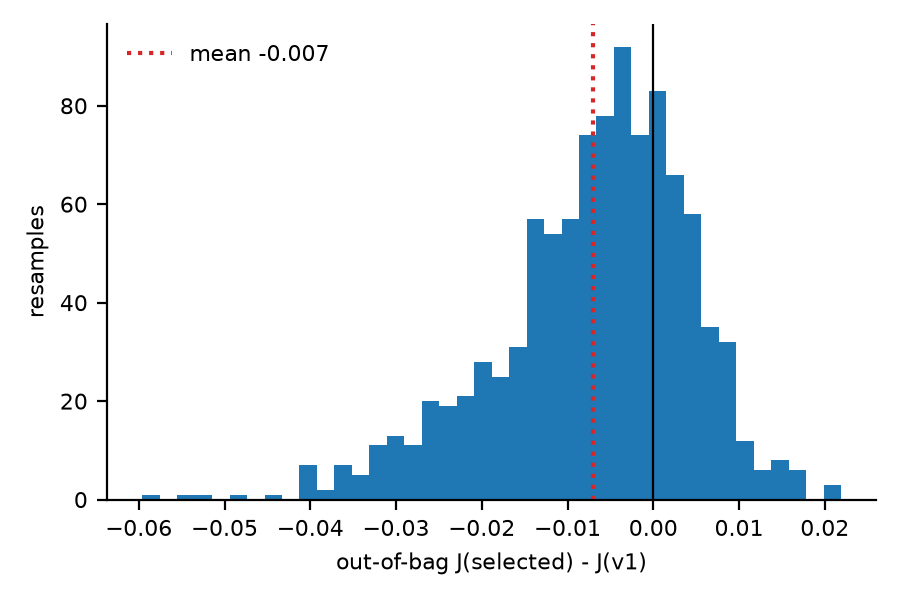
\includegraphics[width=0.9\textwidth]{fig_oob_difference.png}\caption{Paired out-of-bag difference between the selected weighting and v1 over 1,000 resamples.}\label{figall:fig_oob_difference}\end{figure}
\noindent{\small \textbf{What it encodes.} For each of the 1,000 resamples, the out-of-bag $J$ of the selected weighting minus the out-of-bag $J$ of v1; the vertical line is zero. \textbf{How to read it.} Mass to the right of zero means the search beat v1 on held-out items in that resample. The mean and the 2.5--97.5 percentile interval are the paired test. \textbf{What it shows.} The distribution is centred at -0.007 with the interval straddling zero; the selected weighting is ahead in only 28\,\% of resamples.}
\clearpage

\begin{figure}[htbp]\centering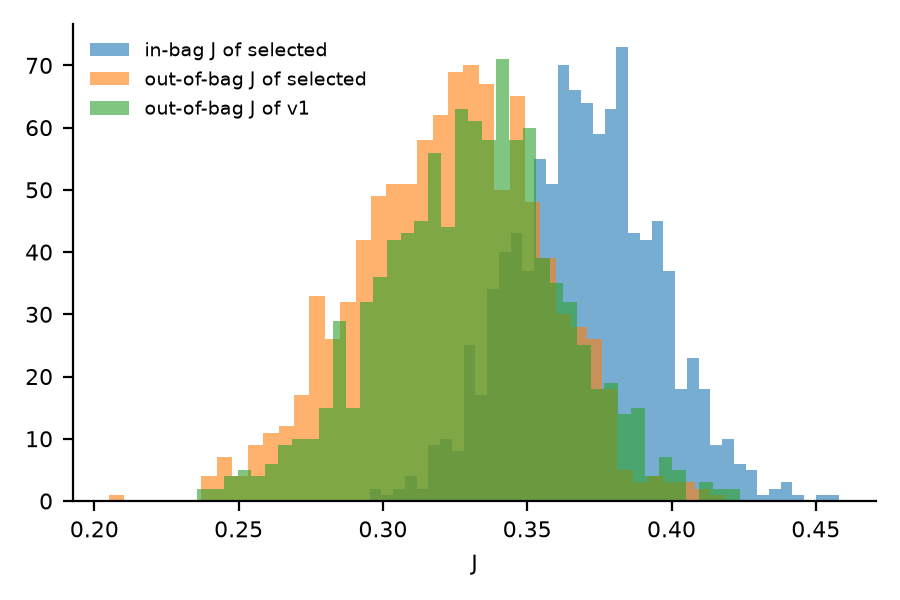
\includegraphics[width=0.9\textwidth]{fig_optimism_distributions.png}\caption{Distributions behind the optimism gap: in-bag $J$ of the selected weighting, its out-of-bag $J$, and v1's out-of-bag $J$.}\label{figall:fig_optimism_distributions}\end{figure}
\noindent{\small \textbf{What it encodes.} The three bootstrap distributions behind the optimism gap, as histograms over the 1,000 resamples. \textbf{How to read it.} The in-bag distribution of the selected weighting (shifted right) is what an un-validated search would report; the two out-of-bag distributions overlap almost completely. \textbf{What it shows.} The shift is the selection effect itself, about 0.047 of $J$; the overlap of the out-of-bag distributions is why no weighting can be declared better than v1.}
\clearpage

\begin{figure}[htbp]\centering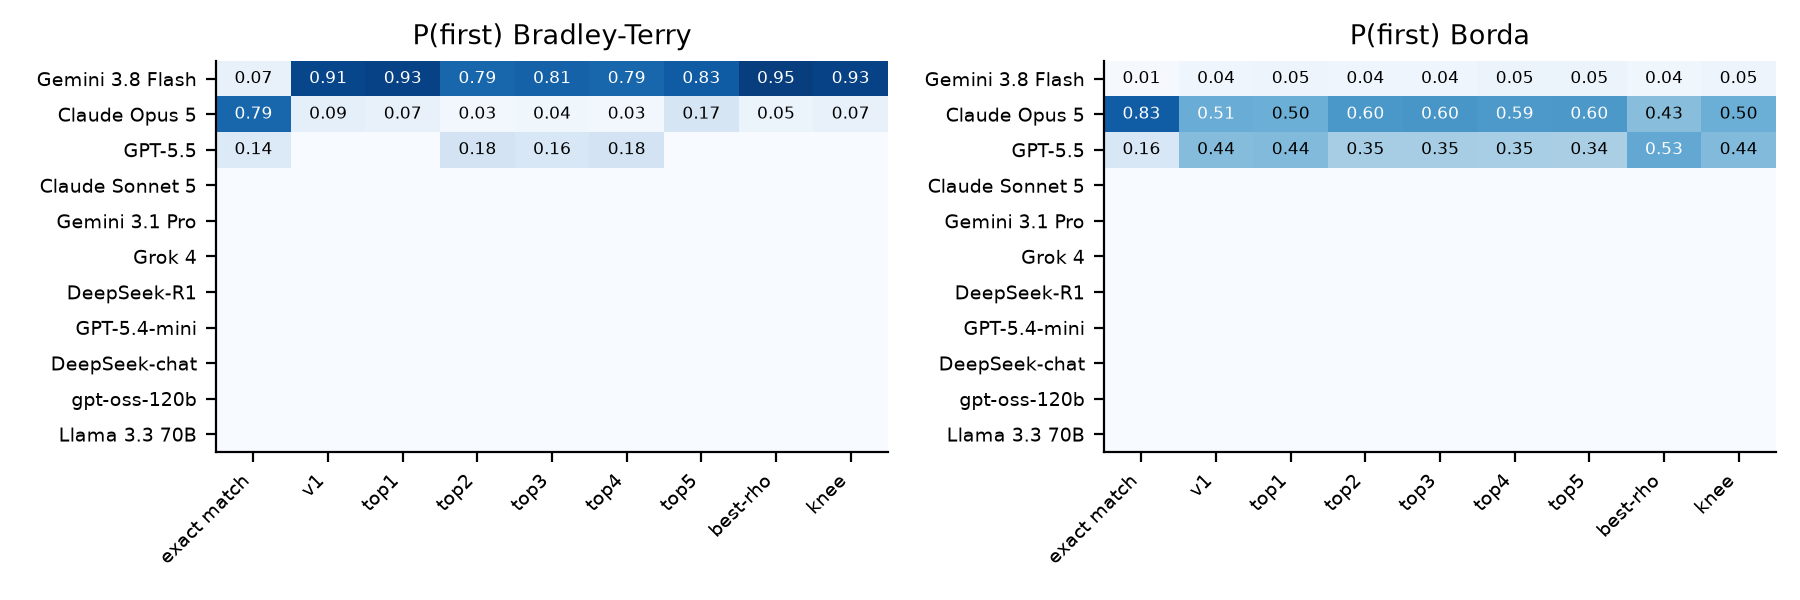
\includegraphics[width=0.9\textwidth]{fig_p_first.png}\caption{Bootstrap probability of first place for every model under every rule, by pooling method.}\label{figall:fig_p_first}\end{figure}
\noindent{\small \textbf{What it encodes.} The bootstrap probability of first place for every model under every rule, by Bradley--Terry (left) and Borda (right) pooling. \textbf{How to read it.} Each column sums to one. A dark cell is a confident first place; a column with several mid-tone cells is a contested one. \textbf{What it shows.} Bradley--Terry is nearly certain about Gemini Flash under the graded rules and about Opus under exact match; Borda divides first place between Opus and GPT-5.5 under most rules. The pooling method, not only the scoring rule, decides the headline winner.}
\clearpage

\begin{figure}[htbp]\centering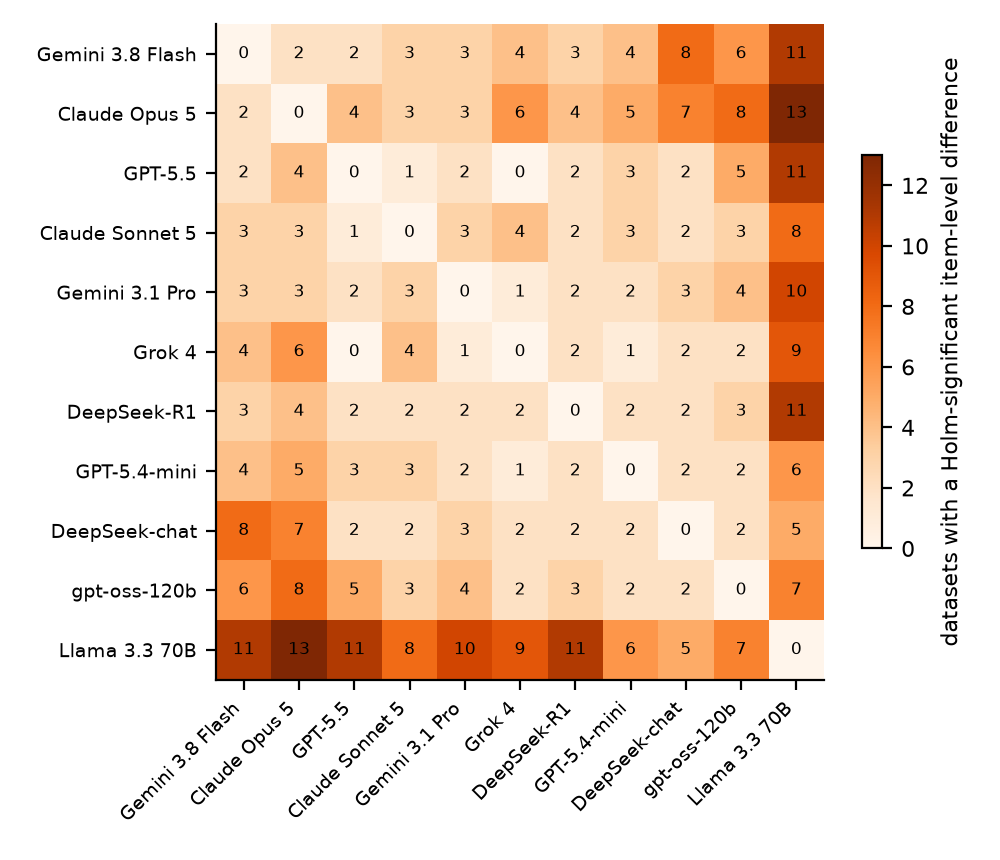
\includegraphics[width=0.9\textwidth]{fig_pairwise_significance_v1.png}\caption{Number of datasets (of 31) in which the per-item paired test separates each pair of models under v1 (Holm within dataset).}\label{figall:fig_pairwise_significance_v1}\end{figure}
\noindent{\small \textbf{What it encodes.} For each pair of models, the number of datasets (of 31) in which a Holm-corrected per-item paired test separates them under v1. \textbf{How to read it.} A high count is a pair separated on many datasets; zero is a pair never separated at the item level even where the cross-dataset test suggests a difference. \textbf{What it shows.} The pairs involving the bottom two models are separated on many datasets; pairs inside the top group are separated on few. Item-level evidence agrees with the Friedman picture.}
\clearpage

\begin{figure}[htbp]\centering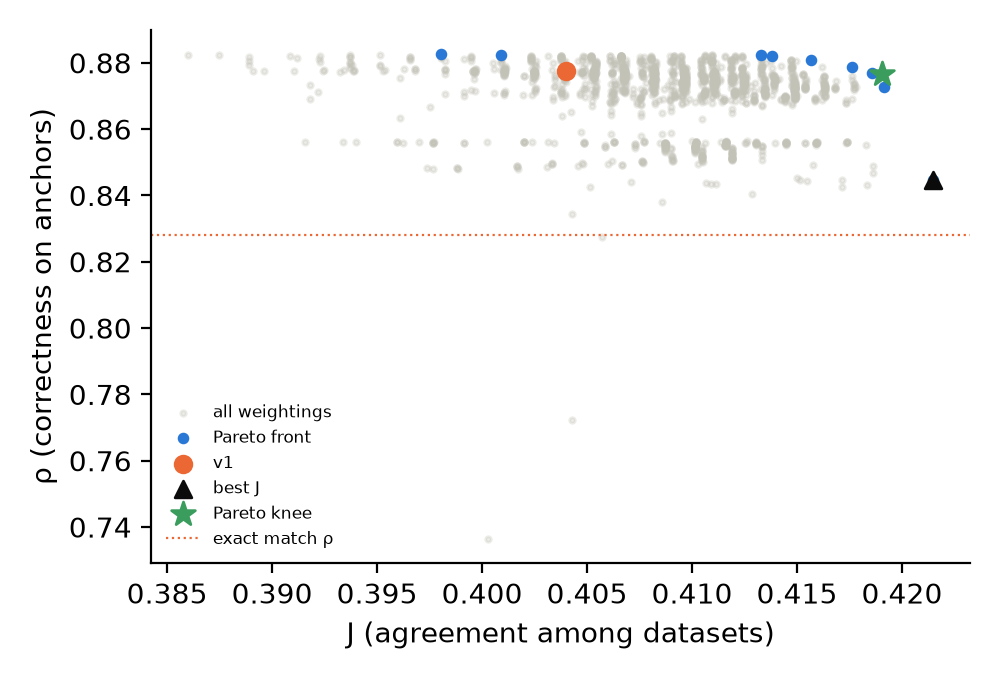
\includegraphics[width=0.9\textwidth]{fig_pareto.png}\caption{Agreement $J$ against anchor correctness $\rho$ for every weighting.}\label{figall:fig_pareto}\end{figure}
\noindent{\small \textbf{What it encodes.} Every weighting placed by its agreement objective $J$ (horizontal) and its Spearman $\rho$ against the known utility of 31,380 synthetic answers (vertical); the Pareto front and the named points (v1, best $J$, best $\rho$, knee) are marked. \textbf{How to read it.} If agreement and correctness pulled together, the cloud would rise to the upper right. A front that bends away means the two criteria trade off. \textbf{What it shows.} The best-$J$ weighting is among the worst by $\rho$ (0.876) while v1 (0.878) sits near the $\rho$ optimum (0.883); across the lattice $J$ and $\rho$ correlate -0.23. Agreement is not correctness, and v1 is close to the correct end.}
\clearpage

\begin{figure}[htbp]\centering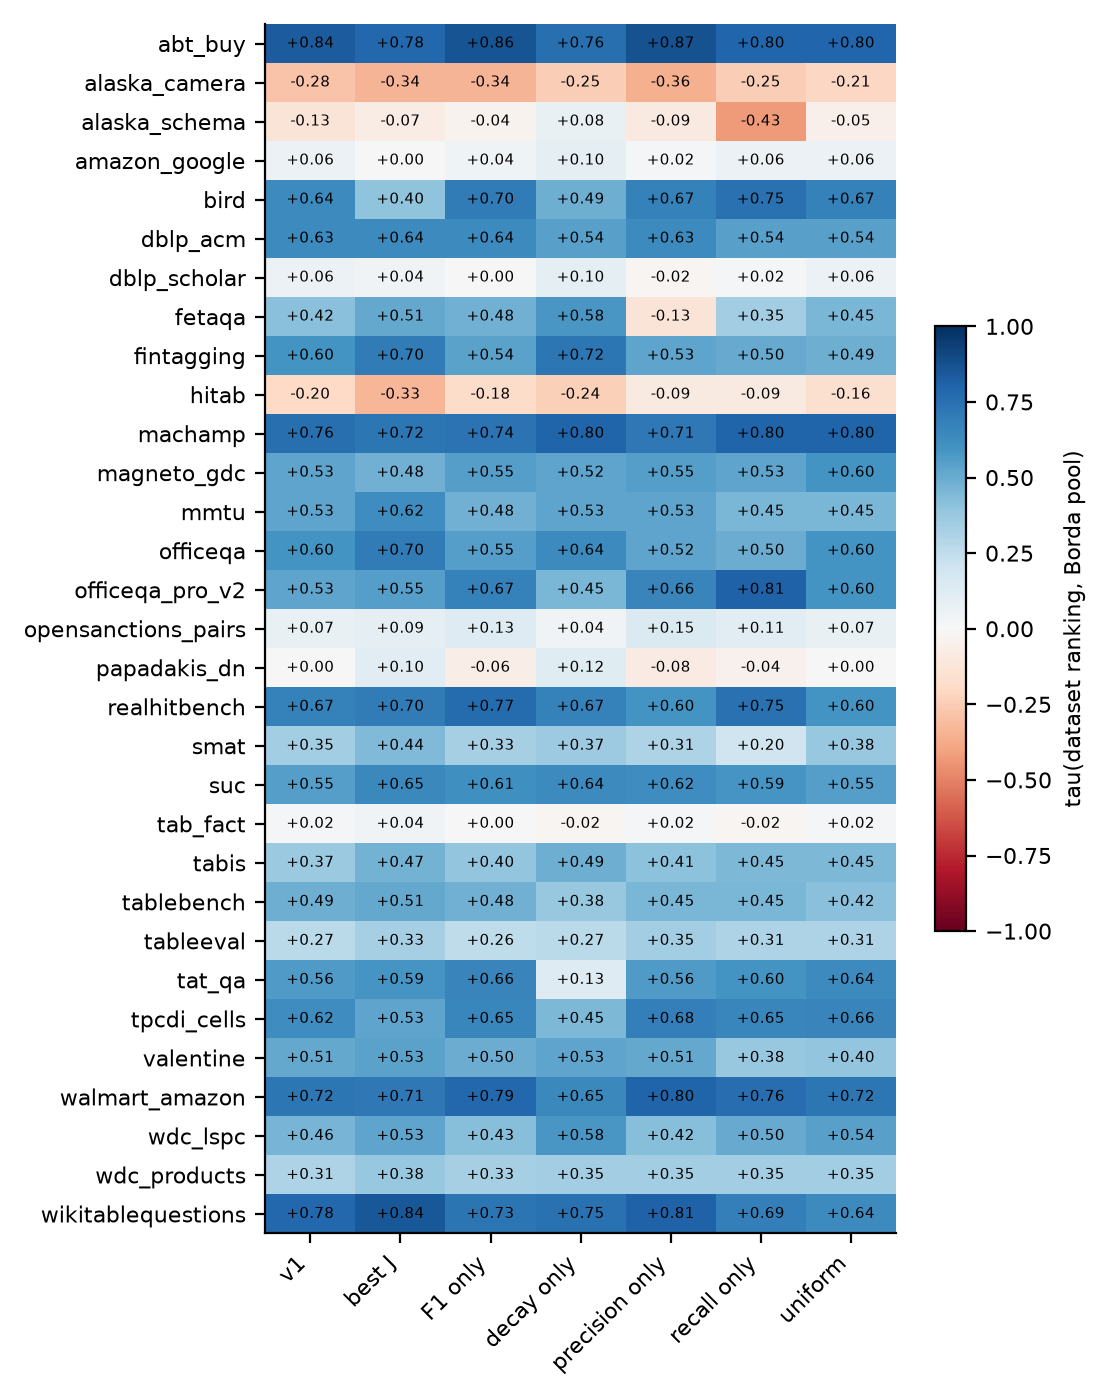
\includegraphics[width=0.9\textwidth]{fig_per_dataset_tau_rules.png}\caption{Per-dataset Kendall $\tau$ to the Borda pool under v1, the best weighting, the four single-ingredient corners and the uniform mix.}\label{figall:fig_per_dataset_tau_rules}\end{figure}
\noindent{\small \textbf{What it encodes.} Rows are the 31 datasets; columns are named weightings (v1, the best, the four corners, the uniform mix); each cell is that dataset's Kendall $\tau$ to the pooled ranking under that weighting (blue positive, red negative). $J$ is the column mean. \textbf{How to read it.} A row that is red in every column is a dataset whose model ranking runs against the consensus whatever the weights; a column that is uniformly bluer than the others would be a weighting that genuinely improves agreement. \textbf{What it shows.} Rows differ far more than columns: the same 3 datasets are negative under every weighting and the same high-agreement datasets are blue everywhere. The weights redistribute a little $\tau$ between datasets; they do not change which datasets agree.}
\clearpage

\begin{figure}[htbp]\centering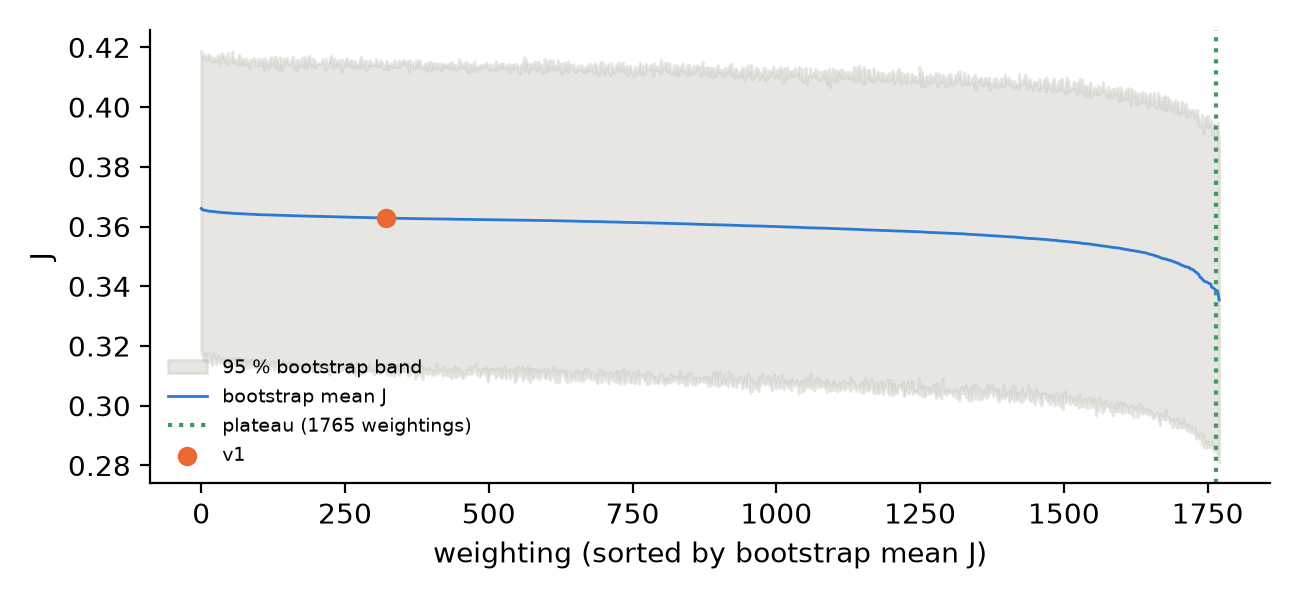
\includegraphics[width=0.9\textwidth]{fig_plateau.png}\caption{Bootstrap band over sorted weightings and the plateau boundary.}\label{figall:fig_plateau}\end{figure}
\noindent{\small \textbf{What it encodes.} Weightings sorted by full-data $J$ (horizontal) with the 95\,\% bootstrap band of each (shaded) and the plateau boundary: the set of weightings not significantly below the best in a paired bootstrap test. \textbf{How to read it.} A weighting is in the plateau when its band overlaps the best's in the paired sense; the boundary is where $p$ drops below .05. \textbf{What it shows.} 1,749 of 1,771 weightings are in the plateau and v1 is inside it ($p$ = 0.63); only the extreme precision-free, decay-dominated corner falls out. The practical plateau (within 0.02 of the best) holds 1,731 weightings.}
\clearpage

\begin{figure}[htbp]\centering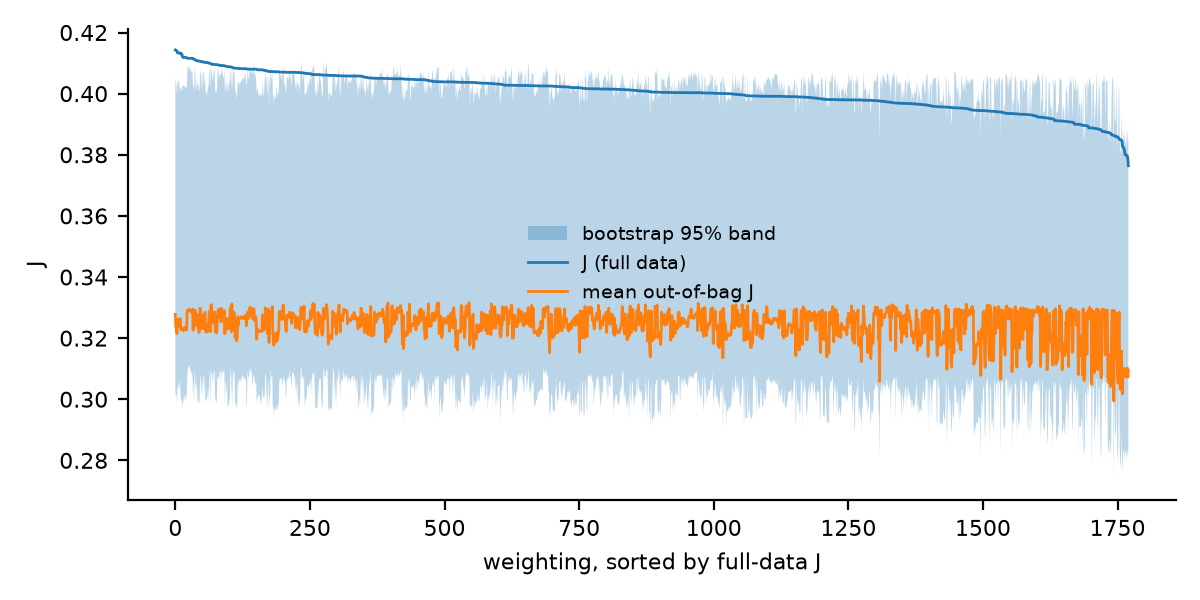
\includegraphics[width=0.9\textwidth]{fig_plateau_oob.png}\caption{Full-data $J$, bootstrap band and mean out-of-bag $J$ for every weighting in rank order.}\label{figall:fig_plateau_oob}\end{figure}
\noindent{\small \textbf{What it encodes.} Three curves over the sorted weightings: full-data $J$, the bootstrap mean with its band, and the mean out-of-bag $J$ when each weighting is evaluated on items it was not selected on. \textbf{How to read it.} The vertical distance between the full-data curve and the out-of-bag curve is the optimism for every weighting, not only the winner. If the out-of-bag curve were steep, some weightings would be reliably better on new items. \textbf{What it shows.} The out-of-bag curve is flat and noisy across the entire lattice: the ordering of weightings on the full data does not reproduce on held-out items.}
\clearpage

\begin{figure}[htbp]\centering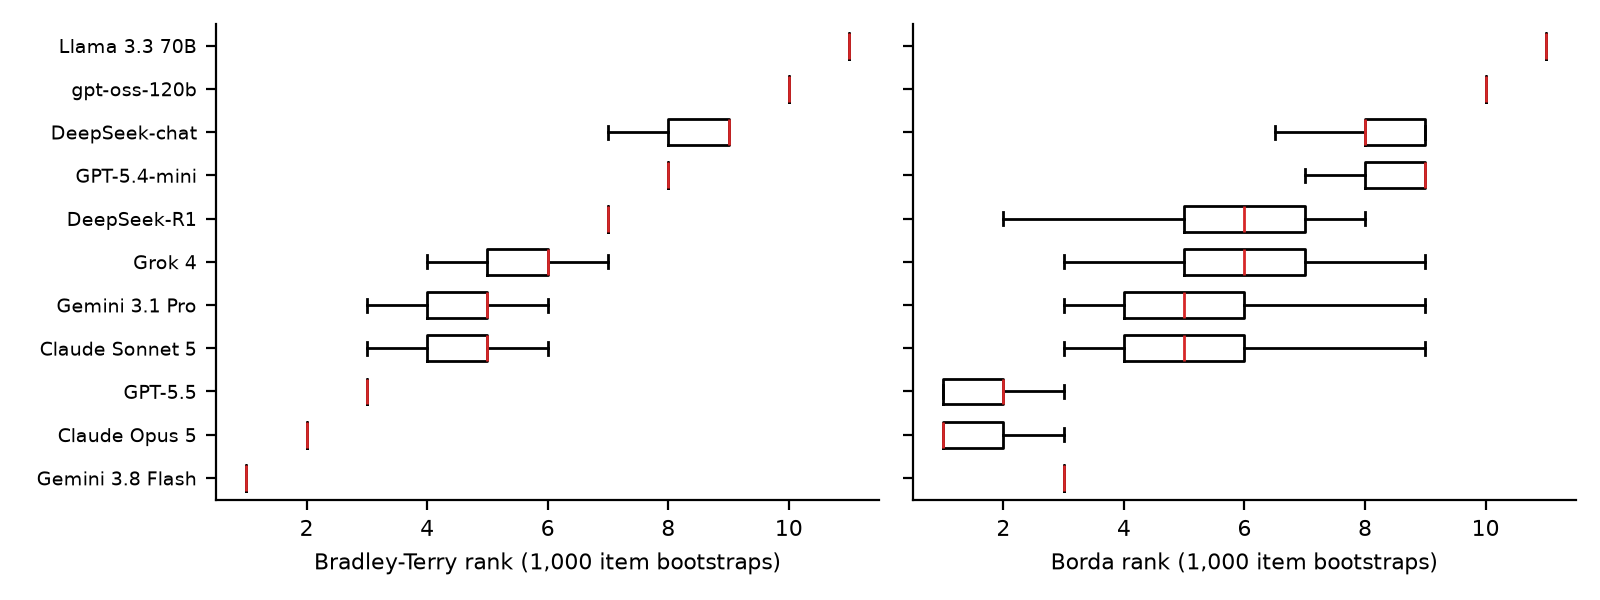
\includegraphics[width=0.9\textwidth]{fig_rank_bootstrap_v1.png}\caption{Bootstrap distribution of each model's rank under v1 (1,000 item resamples).}\label{figall:fig_rank_bootstrap_v1}\end{figure}
\noindent{\small \textbf{What it encodes.} For each model, the distribution of its Bradley--Terry rank (left) and Borda rank (right) over 1,000 item bootstraps under v1. \textbf{How to read it.} A narrow box is a rank the data pin down; a wide box is a rank that depends on which items are drawn. Overlapping boxes are models whose order is not established. \textbf{What it shows.} Bradley--Terry pins Gemini Flash to first (P = 0.91) and the last two to their places; the middle four overlap. Borda spreads first place over three models, because it counts dataset-level ranks rather than item-level wins.}
\clearpage

\begin{figure}[htbp]\centering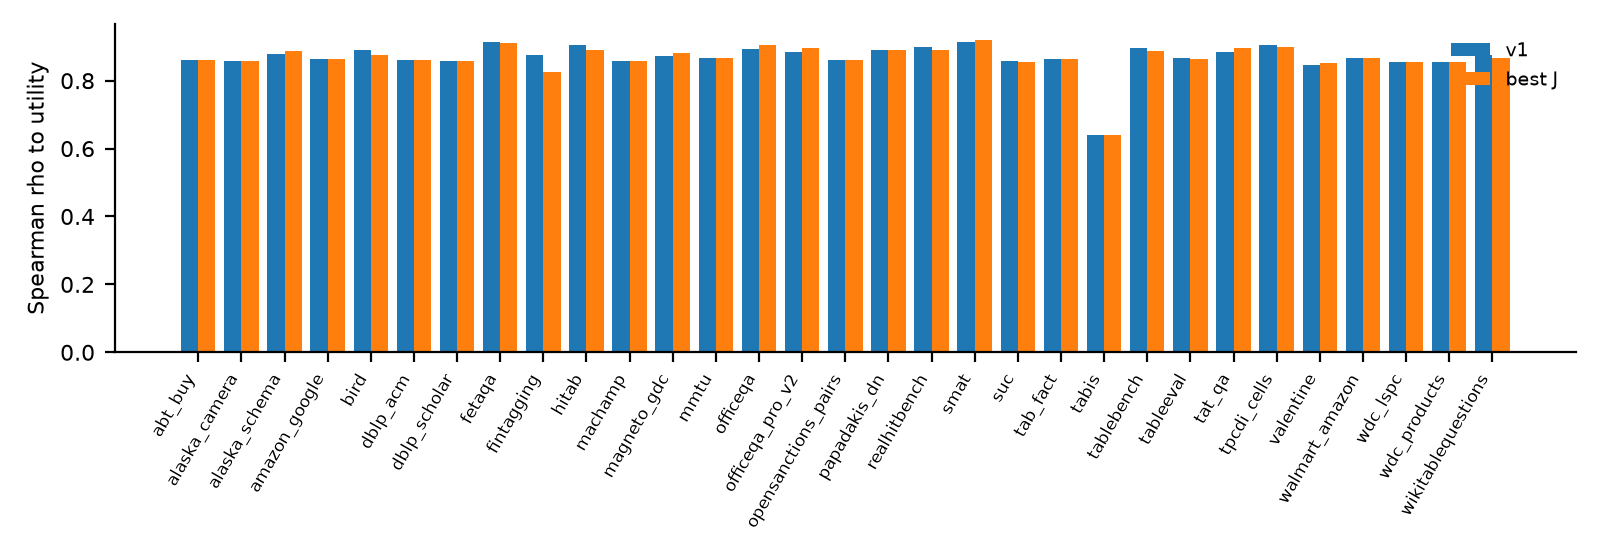
\includegraphics[width=0.9\textwidth]{fig_rho_per_dataset.png}\caption{Anchor correctness (Spearman $\rho$ between composite and known utility) per dataset under v1, the best-$J$ and the best-$\rho$ weightings.}\label{figall:fig_rho_per_dataset}\end{figure}
\noindent{\small \textbf{What it encodes.} Spearman $\rho$ between score and known utility computed within each dataset's anchors, under v1, the best-$J$ and the best-$\rho$ weightings. \textbf{How to read it.} Datasets where the three bars differ are where the weighting changes how well the judge grades answers; equal bars mean the weighting is irrelevant there. \textbf{What it shows.} v1 and best-$\rho$ are close everywhere; best-$J$ falls behind on the numeric and list-answer datasets, which is where decay-only weighting loses the partial credit that token overlap provides.}
\clearpage

\begin{figure}[htbp]\centering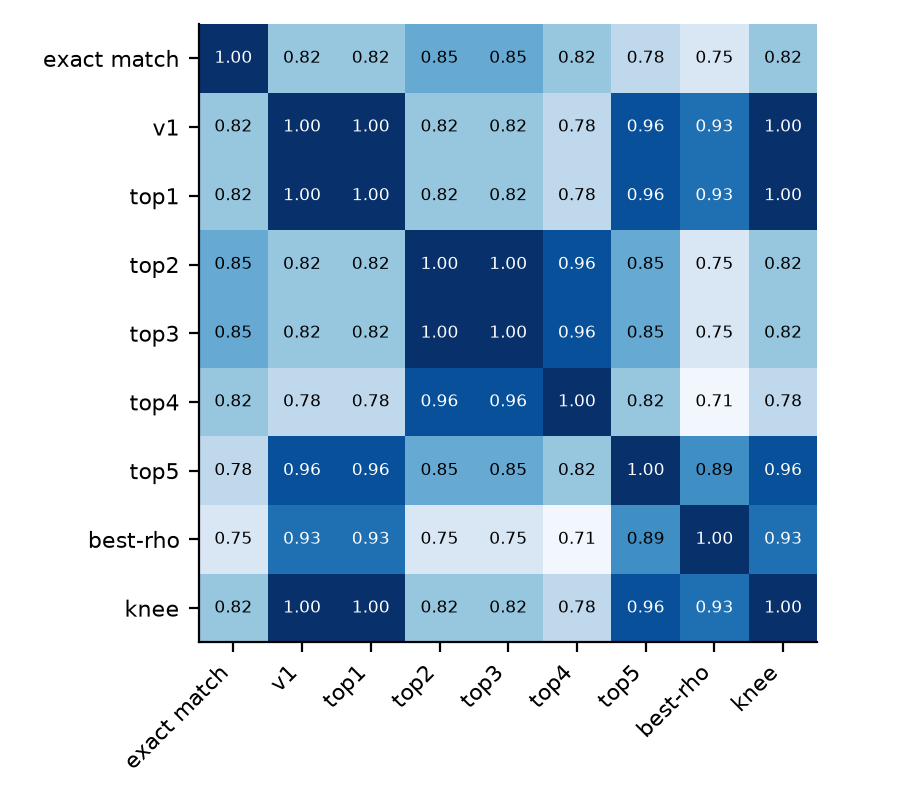
\includegraphics[width=0.9\textwidth]{fig_rule_agreement.png}\caption{Kendall $\tau$ between the Bradley--Terry rankings produced by each pair of rules.}\label{figall:fig_rule_agreement}\end{figure}
\noindent{\small \textbf{What it encodes.} Kendall $\tau$ between the Bradley--Terry rankings produced by each pair of rules. \textbf{How to read it.} 1.00 means identical rankings; values near 0.8 mean a few adjacent swaps. \textbf{What it shows.} The graded rules agree with each other at 0.71 or above; exact match is the outlier because it ranks the reasoning-heavy models differently. Changing the weights inside the plateau does not change the leaderboard beyond adjacent swaps.}
\clearpage

\begin{figure}[htbp]\centering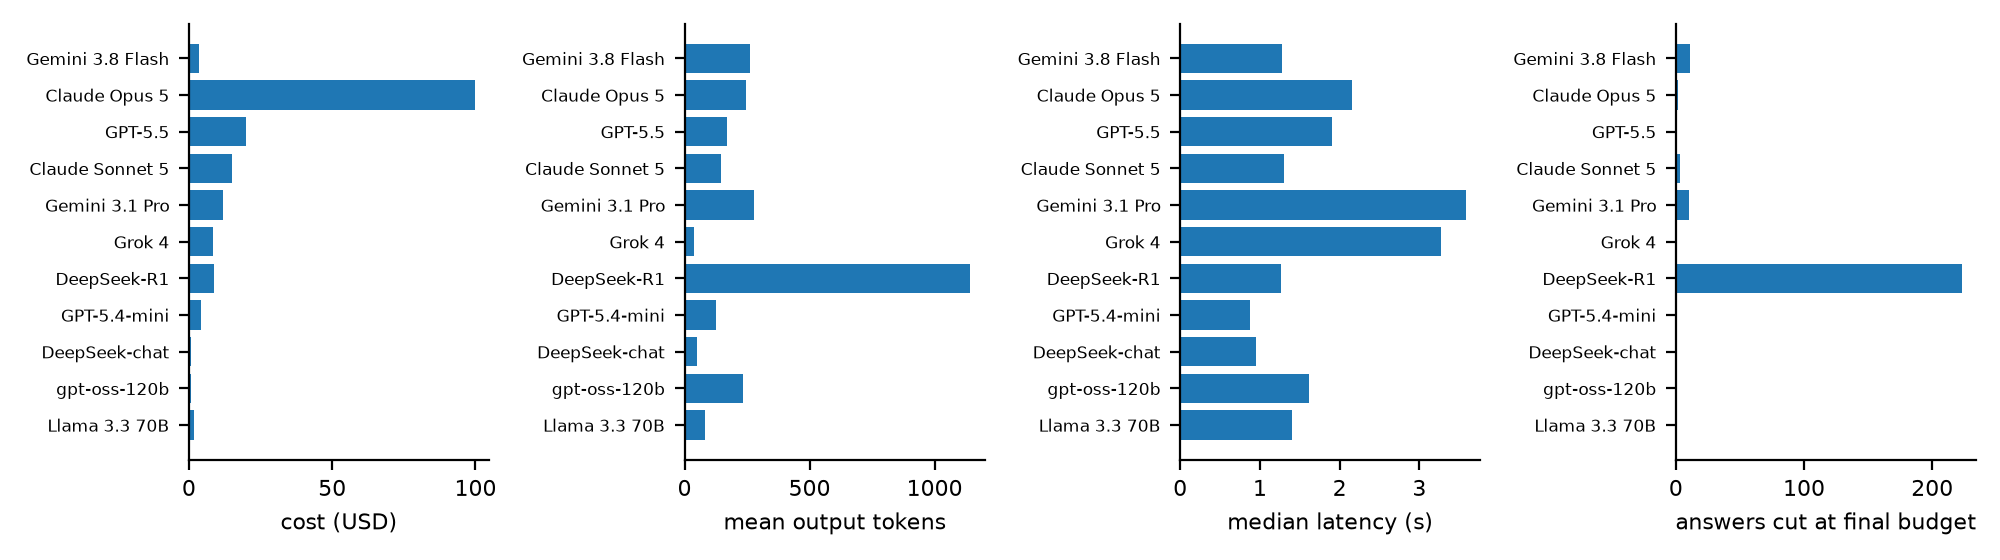
\includegraphics[width=0.9\textwidth]{fig_run_facts.png}\caption{Run facts per model from the prediction cache: cost, output length, latency and answers still cut off at the final budget.}\label{figall:fig_run_facts}\end{figure}
\noindent{\small \textbf{What it encodes.} Per model: total API cost for the suite, mean output tokens, median latency, and the number of answers still cut off at the final budget. \textbf{How to read it.} Cost and output length are the price of a model's position; cut-offs are the answers scored as given because the model did not finish. \textbf{What it shows.} One model accounts for most of the bill, output length varies by more than an order of magnitude, and the residual cut-offs are concentrated in the reasoning model that writes its chain of thought into the output budget.}
\clearpage

\begin{figure}[htbp]\centering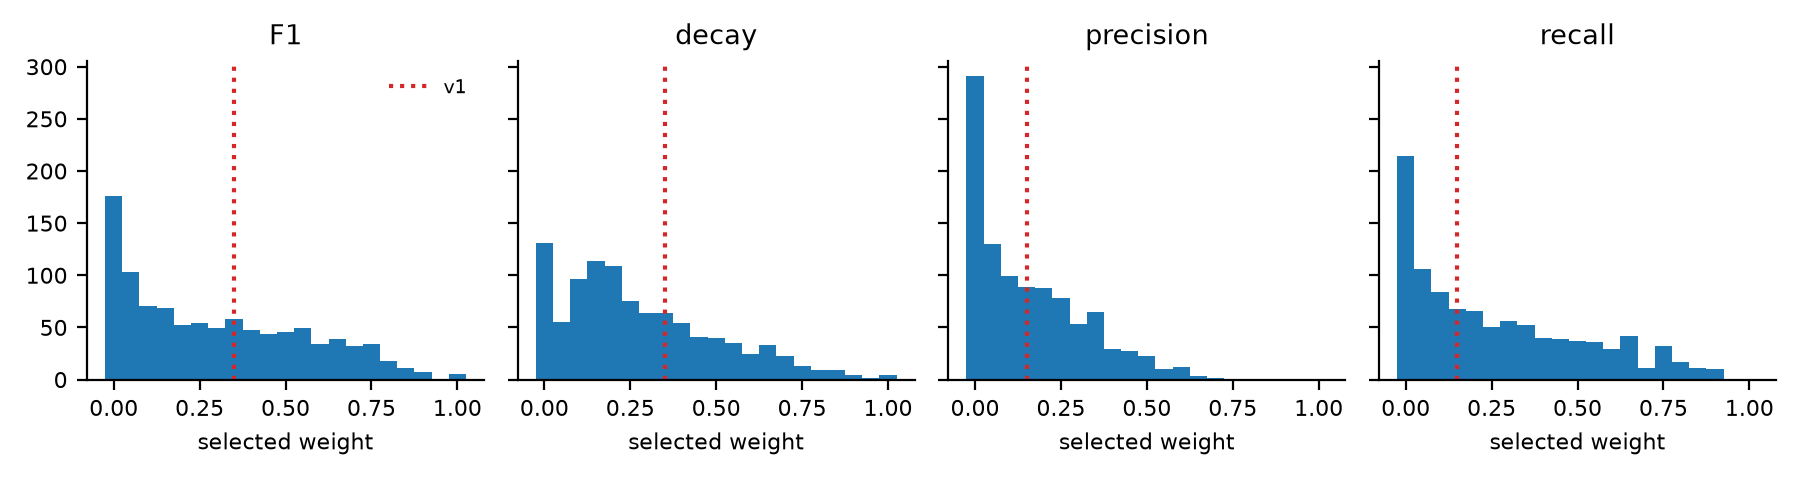
\includegraphics[width=0.9\textwidth]{fig_selected_weights.png}\caption{Weights selected as best on the in-bag items across 1,000 bootstrap resamples; dotted line = v1.}\label{figall:fig_selected_weights}\end{figure}
\noindent{\small \textbf{What it encodes.} Four histograms: the weight on each ingredient of the weighting selected as in-bag best, over the 1,000 resamples; the dotted line is v1's value. \textbf{How to read it.} If the data pointed to a specific weighting, each histogram would be a narrow spike. Spread across the whole range means the ``best'' weighting depends on which items happen to be drawn. \textbf{What it shows.} 624 different weightings win across the resamples, and every weight spreads over most of its range (standard deviations f1 0.26, decay 0.22, precision 0.16, recall 0.25). The selection is close to uniform over the simplex.}
\clearpage

\begin{figure}[htbp]\centering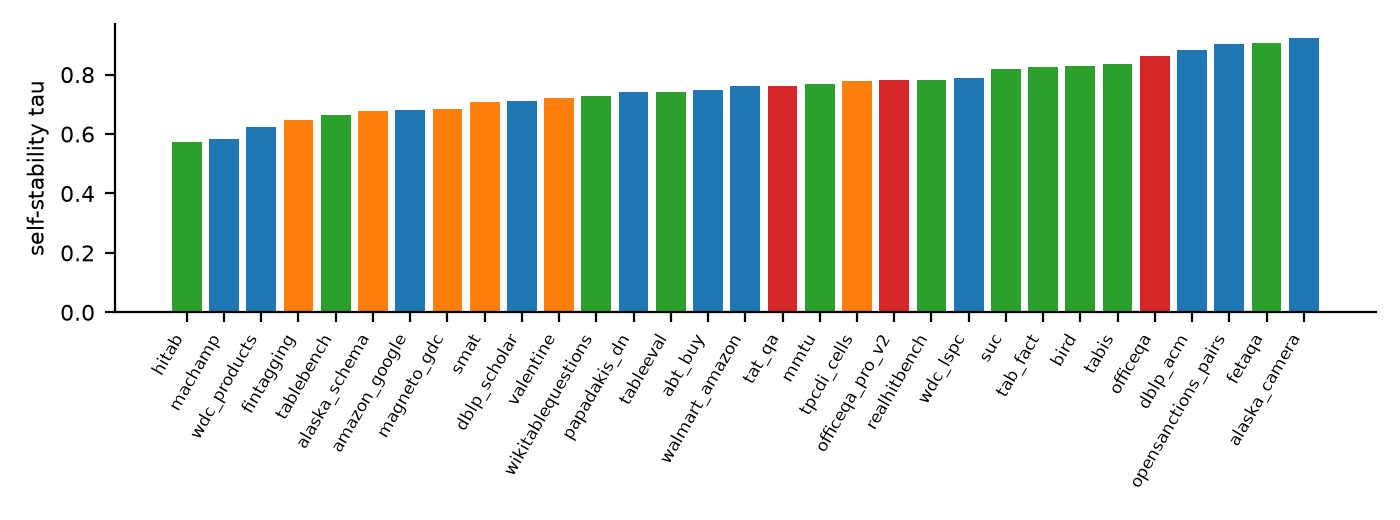
\includegraphics[width=0.9\textwidth]{fig_self_stability.png}\caption{Self-stability of each dataset's model ranking (Kendall $\tau$ between bootstrap halves) under v1.}\label{figall:fig_self_stability}\end{figure}
\noindent{\small \textbf{What it encodes.} For each dataset, the Kendall $\tau$ between the model rankings obtained on two bootstrap halves of its items (self-stability). \textbf{How to read it.} A value near 1 means the dataset's ranking is reproducible from its own items; a low value means its ranking is driven by a few items. \textbf{What it shows.} Self-stability ranges from 0.57 (hitab) to 0.92 (alaska\_camera). Low-stability sets are the ones whose disagreement with the consensus is partly noise.}
\clearpage

\begin{figure}[htbp]\centering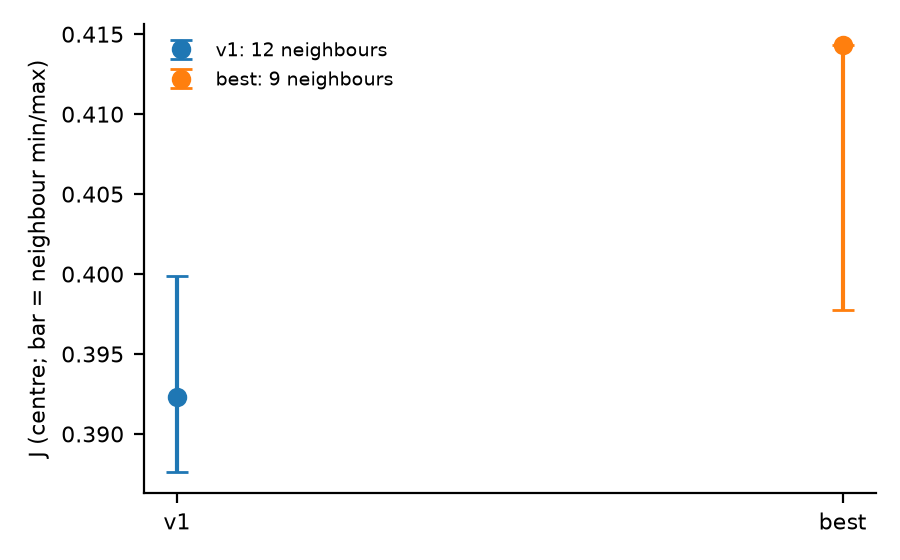
\includegraphics[width=0.9\textwidth]{fig_sensitivity.png}\caption{One-step sensitivity: $J$ at v1 and at the best weighting with the range over all lattice neighbours one 0.05 move away.}\label{figall:fig_sensitivity}\end{figure}
\noindent{\small \textbf{What it encodes.} For v1 and for the best weighting: the $J$ at the point and the range of $J$ over all neighbours one lattice step (0.05) away. \textbf{How to read it.} A long bar would mean a knife-edge optimum; a short bar means the neighbourhood is flat. \textbf{What it shows.} One step moves $J$ by at most 0.012 around v1 and 0.017 around the best: both sit on flat ground, and the best is not a peak but a point on a plateau.}
\clearpage

\begin{figure}[htbp]\centering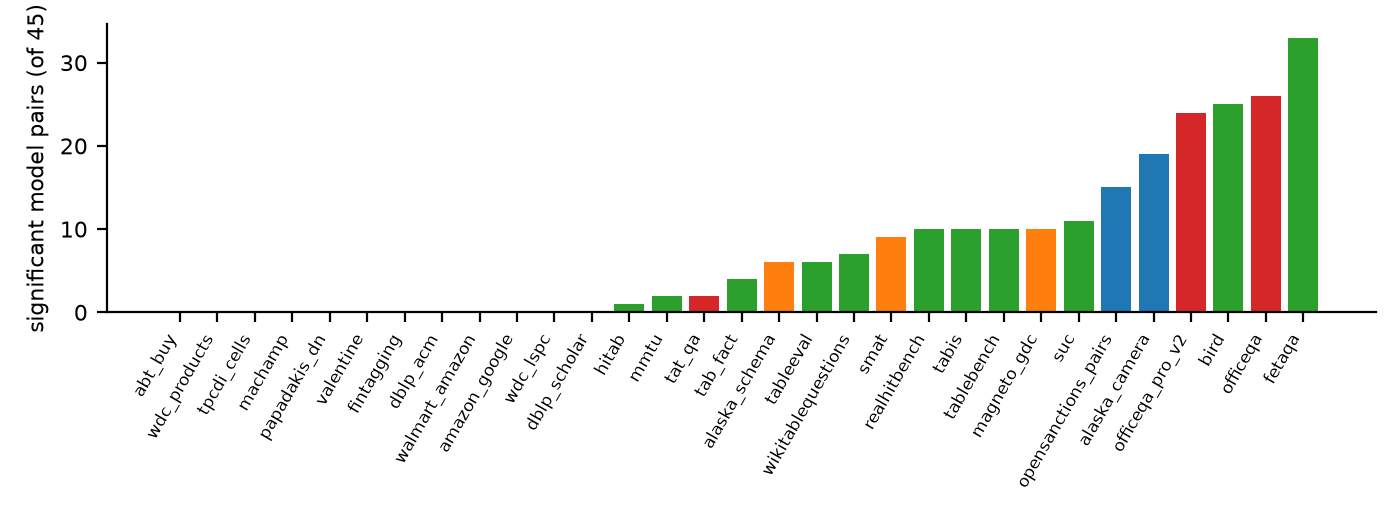
\includegraphics[width=0.9\textwidth]{fig_significant_pairs_per_dataset.png}\caption{How many of the 45 model pairs each dataset separates at the item level under v1 (colour = family).}\label{figall:fig_significant_pairs_per_dataset}\end{figure}
\noindent{\small \textbf{What it encodes.} For each dataset, how many of the 45 model pairs the per-item paired test separates, coloured by family. \textbf{How to read it.} A dataset with zero separates no pair: either every model scores the same or the items are too few for the differences present. High bars are the datasets carrying the leaderboard's statistical power. \textbf{What it shows.} 12 datasets separate no pair, all of them entity-matching or ceiling sets; 4 datasets separate 20 or more, led by FeTaQA and the two OfficeQA sets. Power lives in a dozen table and document sets.}
\clearpage

\begin{figure}[htbp]\centering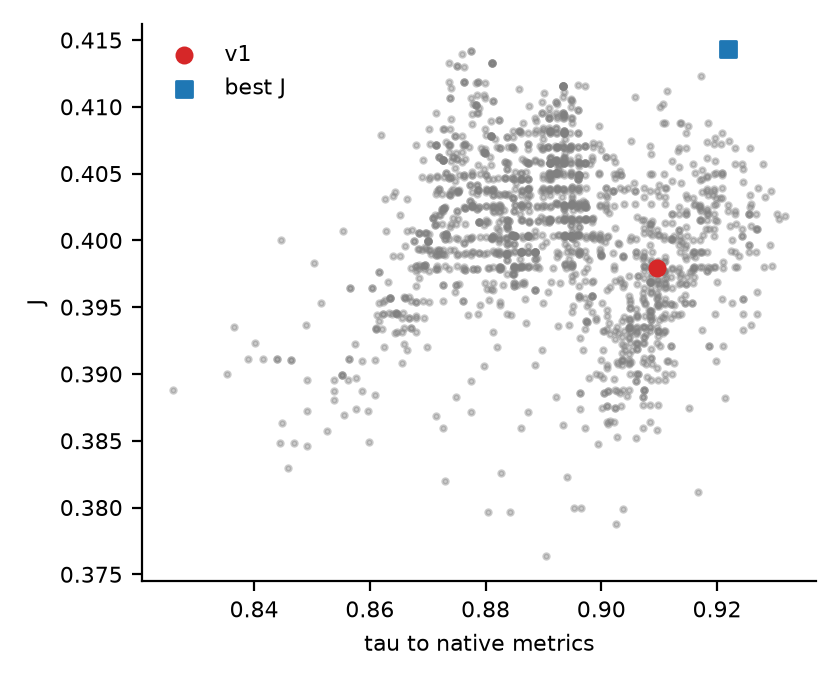
\includegraphics[width=0.9\textwidth]{fig_tau_native_vs_j.png}\caption{Agreement $J$ against Kendall $\tau$ between each weighting's ranking and the native-metric ranking.}\label{figall:fig_tau_native_vs_j}\end{figure}
\noindent{\small \textbf{What it encodes.} Each weighting placed by its agreement with the datasets' own native metrics (horizontal: Kendall $\tau$ between the composite's model ranking and the native-metric ranking) and its $J$ (vertical). \textbf{How to read it.} Points to the right rank the models the way the datasets' own metrics would; points to the top make the datasets agree with each other. A strong diagonal would mean the two criteria coincide. \textbf{What it shows.} The correlation is weak (-0.12); v1 is among the most native-faithful weightings (0.910) while the best-$J$ weighting is slightly less so. Agreement among datasets is a different criterion from fidelity to each dataset's own metric.}
\clearpage

\begin{figure}[htbp]\centering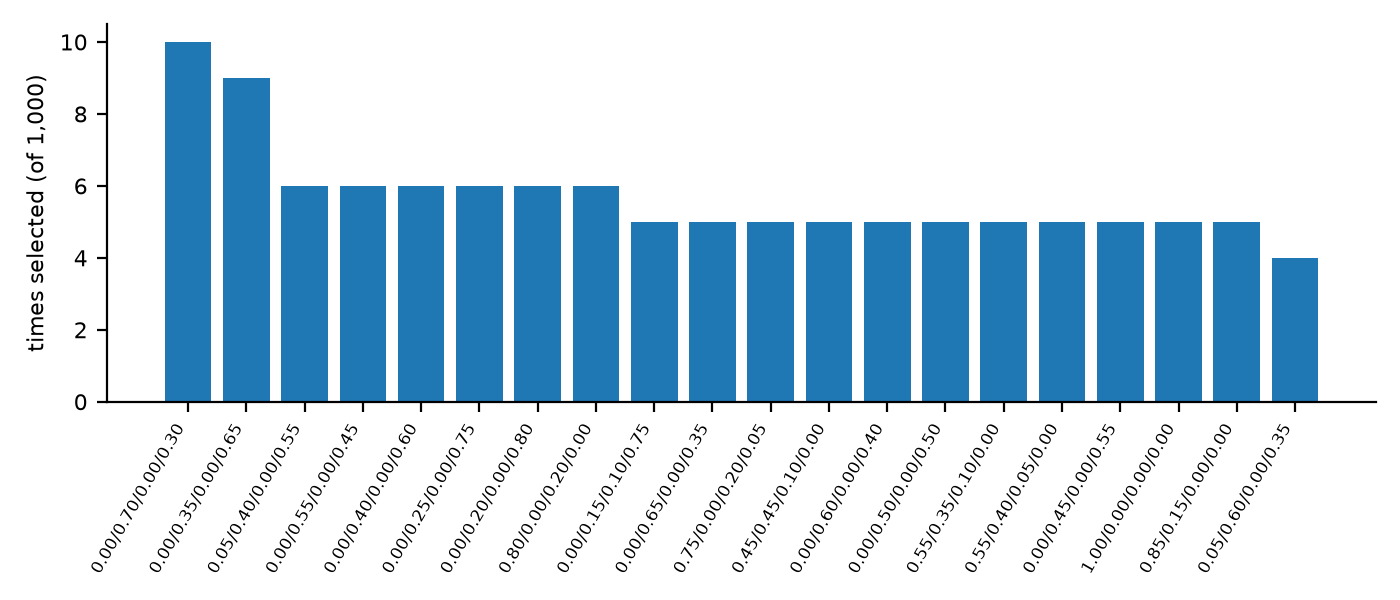
\includegraphics[width=0.9\textwidth]{fig_times_selected.png}\caption{The twenty weightings most often selected as in-bag best (F1 / decay / precision / recall).}\label{figall:fig_times_selected}\end{figure}
\noindent{\small \textbf{What it encodes.} The twenty weightings most often chosen as in-bag best across the 1,000 resamples (labels give F1 / decay / precision / recall). \textbf{How to read it.} A dominant weighting would be selected hundreds of times. A flat bar chart with small counts means no weighting is consistently preferred. \textbf{What it shows.} The most-selected weighting wins only 10 of 1,000 resamples, and the winners include decay-dominated, F1-dominated and recall-dominated points alike.}
\clearpage

\begin{figure}[htbp]\centering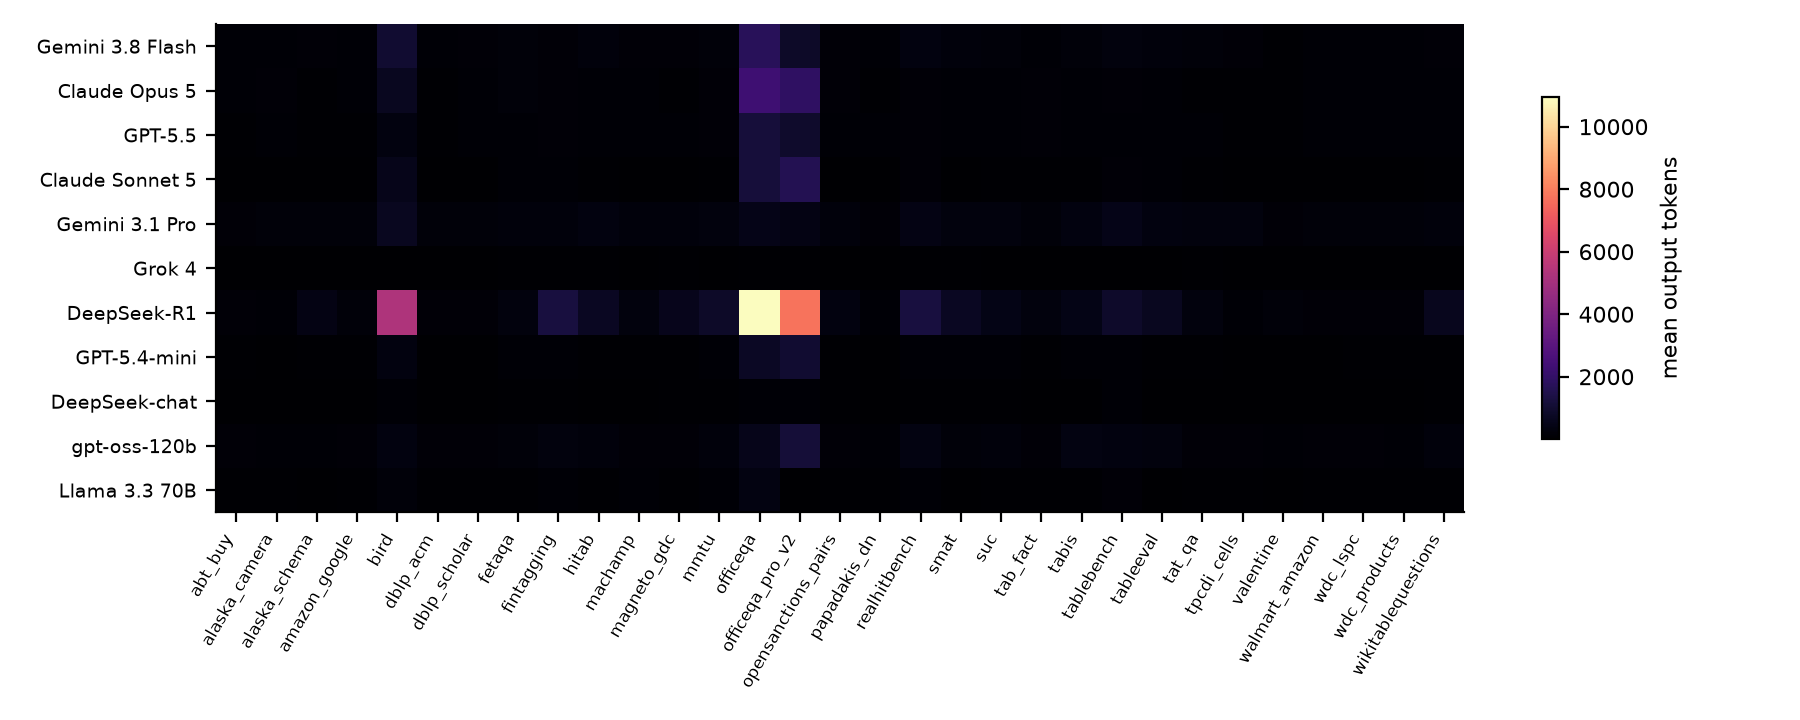
\includegraphics[width=0.9\textwidth]{fig_tokens_heatmap.png}\caption{Mean output tokens per model and dataset.}\label{figall:fig_tokens_heatmap}\end{figure}
\noindent{\small \textbf{What it encodes.} Mean output tokens per model and dataset. \textbf{How to read it.} Columns show which tasks make every model write more (documents and SQL); rows show each model's verbosity. \textbf{What it shows.} The two OfficeQA sets and BIRD draw the longest replies from every model, and the reasoning models write several times more than the rest on the same items. These are the cells where the output budget bites.}
\clearpage

\begin{figure}[htbp]\centering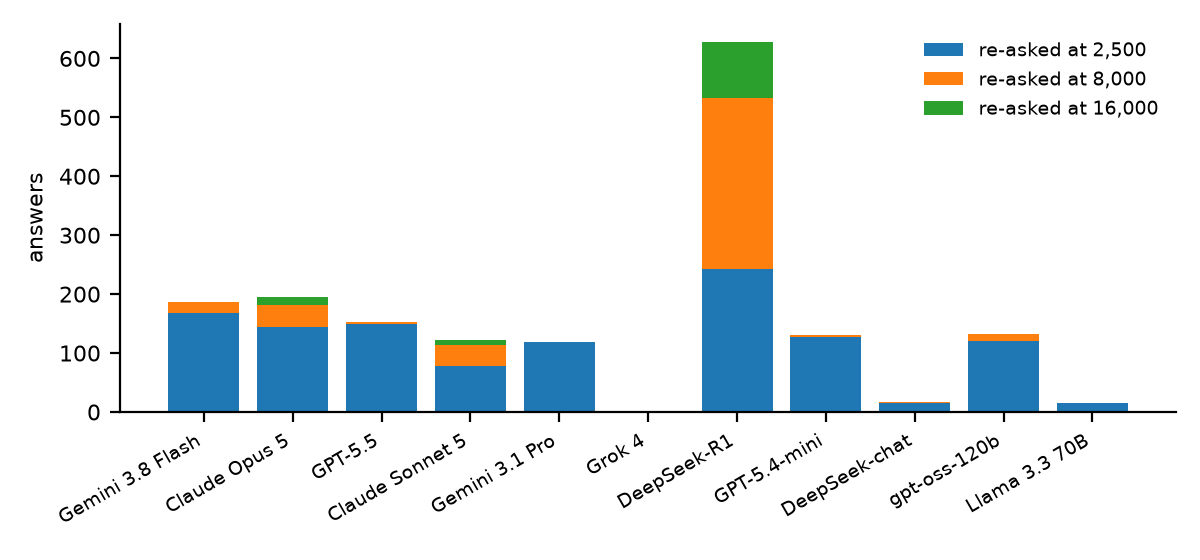
\includegraphics[width=0.9\textwidth]{fig_truncation.png}\caption{Truncation protocol: answers re-asked at 2,500, 8,000 and 16,000 output tokens per model.}\label{figall:fig_truncation}\end{figure}
\noindent{\small \textbf{What it encodes.} Per model, how many answers were re-asked at each stage of the truncation protocol after being cut off without a final line at the previous budget. \textbf{How to read it.} The trigger is mechanical (finish reason ``length'' and no final-answer line), never correctness; a tall bar is a verbose or reasoning-heavy model, not a worse one. \textbf{What it shows.} The reasoning models dominate the re-asks; the short-answer models almost never hit the first budget.}
\clearpage

\begin{figure}[htbp]\centering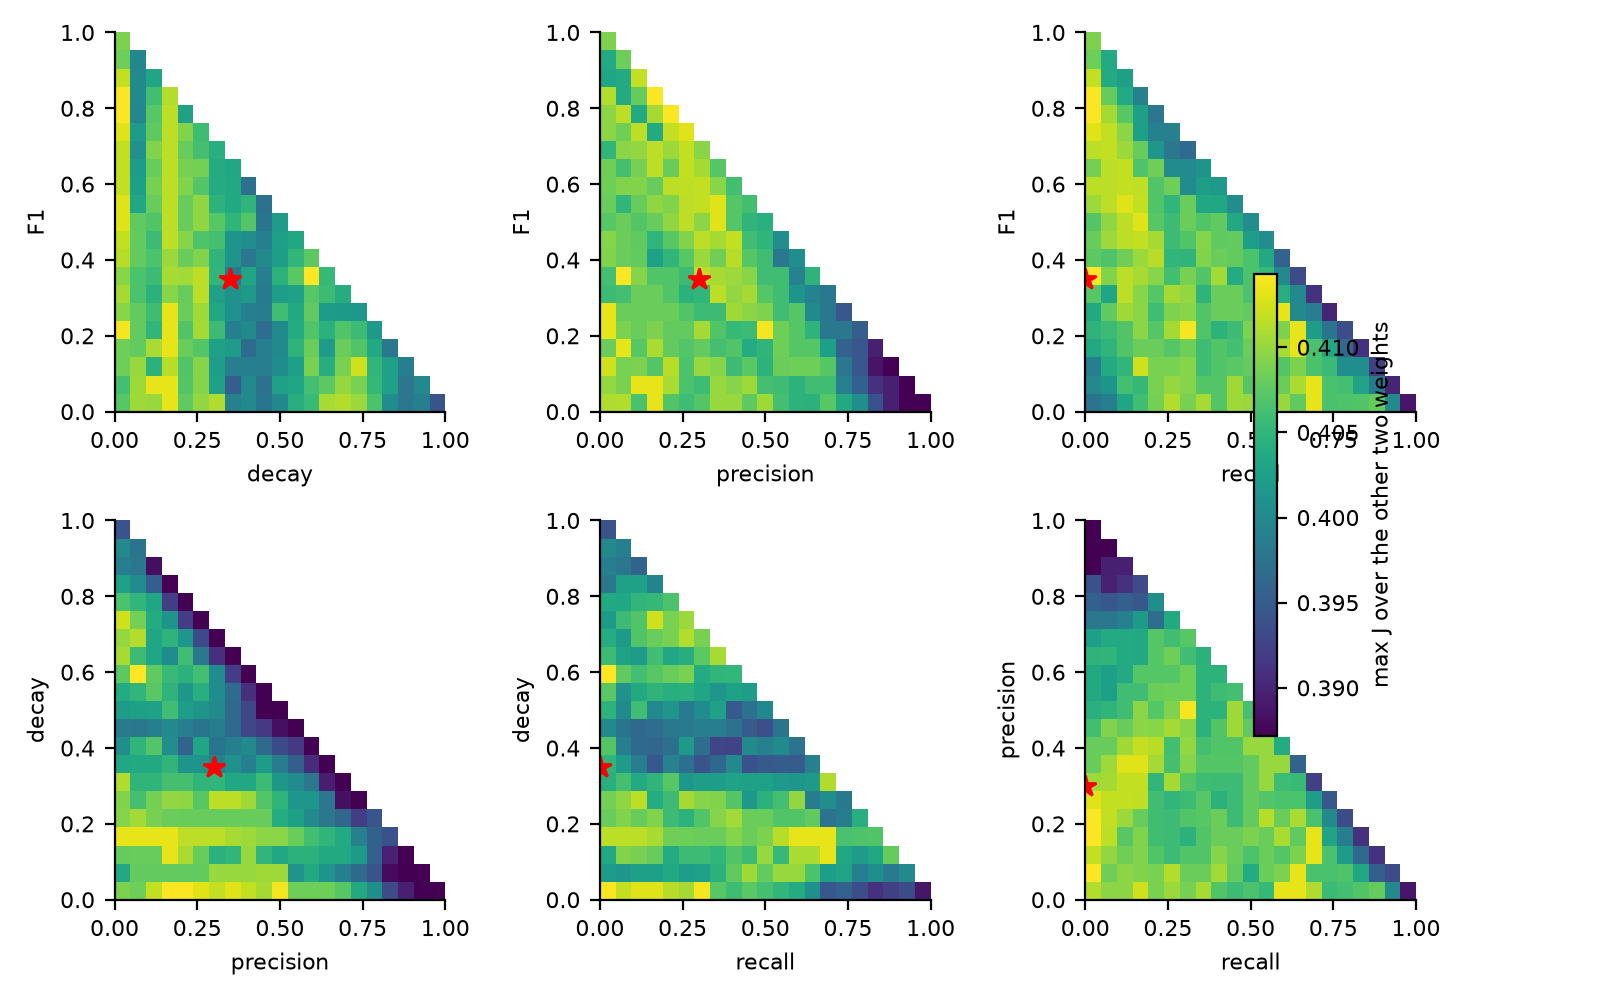
\includegraphics[width=0.9\textwidth]{fig_weight_pairs.png}\caption{Best $J$ attainable for each pair of weight values (maximised over the remaining two weights); red star = v1.}\label{figall:fig_weight_pairs}\end{figure}
\noindent{\small \textbf{What it encodes.} Six heatmaps, one per pair of ingredients; each cell is the best $J$ attainable with those two weights fixed at the cell's values and the other two weights free. The red star is v1. \textbf{How to read it.} A ridge or a hot spot would point to a region of good weightings; a uniform colour means the pair does not constrain $J$. Only the lower-left triangle is feasible because the two weights cannot sum to more than one. \textbf{What it shows.} The feasible triangle is uniformly coloured except for a slightly cooler edge where precision dominates. There is no ridge to follow: the best $J$ is reachable from almost any pair of values.}
\clearpage

\clearpage
\section{All tables}
\label{app:tables}
Every saved table, exported from \texttt{data/}. Each is a separate file under \texttt{tables/}; include any of them in the main text with \texttt{\textbackslash input}.

\begin{table}[htbp]
\centering\scriptsize
\caption{Anchor operators: known utility, mean v1 score, exact-match rate and count.}
\label{tab:anchor_operators}
\setlength{\tabcolsep}{3pt}
\begin{tabular}{p{0.700\linewidth}rrrr}
\toprule
op & utility & v1 & em & n \\
\midrule
no\_\allowbreak{}answer & 0.000 & 0.001 & 0.000 & 3083 \\
wrong\_\allowbreak{}random & 0.000 & 0.097 & 0.041 & 1845 \\
flip & 0.000 & 0.000 & 0.000 & 1238 \\
sign\_\allowbreak{}flip & 0.050 & 0.018 & 0.003 & 632 \\
magnitude & 0.050 & 0.091 & 0.013 & 632 \\
near\_\allowbreak{}miss\_\allowbreak{}large & 0.150 & 0.150 & 0.000 & 632 \\
digit\_\allowbreak{}typo & 0.200 & 0.199 & 0.000 & 632 \\
list\_\allowbreak{}dump & 0.250 & 0.373 & 0.013 & 1845 \\
hedge & 0.300 & 0.493 & 0.192 & 2974 \\
shuffled & 0.400 & 0.652 & 0.009 & 109 \\
near\_\allowbreak{}miss\_\allowbreak{}medium & 0.450 & 0.293 & 0.008 & 632 \\
partial & 0.500 & 0.345 & 0.061 & 1213 \\
superset & 0.600 & 0.467 & 0.045 & 1213 \\
typo & 0.600 & 0.334 & 0.101 & 1104 \\
near\_\allowbreak{}miss\_\allowbreak{}small & 0.750 & 0.405 & 0.097 & 632 \\
paraphrase & 0.950 & 0.965 & 0.930 & 3083 \\
verbose & 1.000 & 1.000 & 0.999 & 3083 \\
identity & 1.000 & 1.000 & 0.999 & 3083 \\
tagged & 1.000 & 1.000 & 0.999 & 3083 \\
unit\_\allowbreak{}variant & 1.000 & 0.898 & 0.837 & 632 \\
\bottomrule
\end{tabular}
\end{table}

\clearpage

\begin{landscape}
\begin{table}[htbp]
\centering\tiny
\caption{Anchor correctness for the labelled rules.}
\label{tab:anchors_rules}
\setlength{\tabcolsep}{3pt}
\resizebox{\linewidth}{!}{%
\begin{tabular}{lrrrrrrrrrrrr}
\toprule
label & rank & w\_\allowbreak{}f1 & w\_\allowbreak{}decay & w\_\allowbreak{}precision & w\_\allowbreak{}recall & J & tau\_\allowbreak{}native & rho & rho\_\allowbreak{}ds & auc & wrong\_\allowbreak{}mean & hedge\_\allowbreak{}gap \\
\midrule
only\_\allowbreak{}f1 & 96 & 1.000 & 0.000 & 0.000 & 0.000 & 0.409 & 0.881 & 0.856 & 0.846 & 0.989 & 0.030 & -0.496 \\
uniform & 806 & 0.250 & 0.250 & 0.250 & 0.250 & 0.401 & 0.897 & 0.875 & 0.866 & 0.994 & 0.033 & -0.480 \\
only\_\allowbreak{}decay & 1513 & 0.000 & 1.000 & 0.000 & 0.000 & 0.394 & 0.910 & 0.772 & 0.804 & 0.991 & 0.040 & -0.595 \\
v1\_\allowbreak{}original & 1602 & 0.350 & 0.350 & 0.150 & 0.150 & 0.392 & 0.910 & 0.878 & 0.868 & 0.994 & 0.034 & -0.506 \\
only\_\allowbreak{}recall & 1703 & 0.000 & 0.000 & 0.000 & 1.000 & 0.389 & 0.826 & 0.736 & 0.741 & 0.989 & 0.030 & -0.244 \\
only\_\allowbreak{}precision & 1744 & 0.000 & 0.000 & 1.000 & 0.000 & 0.386 & 0.845 & 0.848 & 0.839 & 0.989 & 0.031 & -0.587 \\
\bottomrule
\end{tabular}
}
\end{table}
\end{landscape}

\clearpage

\scriptsize
\setlength{\tabcolsep}{3pt}
\begin{longtable}{p{0.446\linewidth}p{0.145\linewidth}rp{0.114\linewidth}p{0.145\linewidth}}
\caption{Coverage rule outcome per dataset.}\label{tab:coverage}\\
\toprule
dataset & answered items & items kept & models used & models dropped \\
\midrule
abt\_\allowbreak{}buy & 100 & 100 & 10 & -- \\
alaska\_\allowbreak{}camera & 100 & 100 & 10 & -- \\
alaska\_\allowbreak{}schema & 93 & 93 & 10 & -- \\
amazon\_\allowbreak{}google & 100 & 100 & 10 & -- \\
bird & 100 & 100 & 10 & -- \\
dblp\_\allowbreak{}acm & 100 & 100 & 10 & -- \\
dblp\_\allowbreak{}scholar & 100 & 100 & 10 & -- \\
fetaqa & 100 & 100 & 10 & -- \\
fintagging & 100 & 100 & 10 & -- \\
hitab & 100 & 100 & 10 & -- \\
machamp & 100 & 100 & 10 & -- \\
magneto\_\allowbreak{}gdc & 100 & 100 & 10 & -- \\
mmtu & 100 & 100 & 10 & -- \\
officeqa & 100 & 100 & 10 & -- \\
officeqa\_\allowbreak{}pro\_\allowbreak{}v2 & 90 & 90 & 10 & -- \\
opensanctions\_\allowbreak{}pairs & 100 & 100 & 10 & -- \\
papadakis\_\allowbreak{}dn & 100 & 100 & 10 & -- \\
realhitbench & 100 & 100 & 10 & -- \\
smat & 100 & 100 & 10 & -- \\
suc & 100 & 100 & 10 & -- \\
tab\_\allowbreak{}fact & 100 & 100 & 10 & -- \\
tabis & 100 & 100 & 10 & -- \\
tablebench & 100 & 100 & 10 & -- \\
tableeval & 100 & 100 & 10 & -- \\
tat\_\allowbreak{}qa & 100 & 100 & 10 & -- \\
tpcdi\_\allowbreak{}cells & 100 & 100 & 10 & -- \\
valentine & 100 & 100 & 10 & -- \\
walmart\_\allowbreak{}amazon & 100 & 100 & 10 & -- \\
wdc\_\allowbreak{}lspc & 100 & 100 & 10 & -- \\
wdc\_\allowbreak{}products & 100 & 100 & 10 & -- \\
wikitablequestions & 100 & 100 & 10 & -- \\
\bottomrule
\end{longtable}
\normalsize

\clearpage

\scriptsize
\setlength{\tabcolsep}{3pt}
\begin{longtable}{p{0.362\linewidth}rp{0.211\linewidth}p{0.227\linewidth}r}
\caption{Datasets: family, items answered, dominant answer type and native metric.}\label{tab:datasets}\\
\toprule
dataset & items & answer\_\allowbreak{}type & native\_\allowbreak{}metric & family \\
\midrule
abt\_\allowbreak{}buy & 100 & boolean & em & EM \\
alaska\_\allowbreak{}camera & 100 & boolean & em & EM \\
alaska\_\allowbreak{}schema & 93 & text & em & SM \\
amazon\_\allowbreak{}google & 100 & boolean & em & EM \\
bird & 100 & numeric & em & TQA \\
dblp\_\allowbreak{}acm & 100 & boolean & em & EM \\
dblp\_\allowbreak{}scholar & 100 & boolean & em & EM \\
fetaqa & 100 & freeform & rouge\_\allowbreak{}l & TQA \\
fintagging & 100 & text & em & SM \\
hitab & 100 & numeric & num\_\allowbreak{}tol & TQA \\
machamp & 100 & boolean & em & EM \\
magneto\_\allowbreak{}gdc & 100 & text & em & SM \\
mmtu & 100 & text & em & TQA \\
officeqa & 100 & numeric & num\_\allowbreak{}tol & FIN \\
officeqa\_\allowbreak{}pro\_\allowbreak{}v2 & 90 & numeric & num\_\allowbreak{}tol & FIN \\
opensanctions\_\allowbreak{}pairs & 100 & boolean & em & EM \\
papadakis\_\allowbreak{}dn & 100 & boolean & em & EM \\
realhitbench & 100 & numeric & num\_\allowbreak{}tol & TQA \\
smat & 100 & text & em & SM \\
suc & 100 & text & em & TQA \\
tab\_\allowbreak{}fact & 100 & boolean & em & TQA \\
tabis & 100 & text & em & TQA \\
tablebench & 100 & numeric & num\_\allowbreak{}tol & TQA \\
tableeval & 100 & numeric & num\_\allowbreak{}tol & TQA \\
tat\_\allowbreak{}qa & 100 & numeric & em & FIN \\
tpcdi\_\allowbreak{}cells & 100 & numeric & num\_\allowbreak{}tol & SM \\
valentine & 100 & text & em & SM \\
walmart\_\allowbreak{}amazon & 100 & boolean & em & EM \\
wdc\_\allowbreak{}lspc & 100 & boolean & em & EM \\
wdc\_\allowbreak{}products & 100 & boolean & em & EM \\
wikitablequestions & 100 & numeric & em & TQA \\
\bottomrule
\end{longtable}
\normalsize

\clearpage

\begin{landscape}
\begin{table}[htbp]
\centering\tiny
\caption{Sampled designs: mean and sd over 20 seeds of every coverage and performance measure.}
\label{tab:designs_full}
\setlength{\tabcolsep}{3pt}
\resizebox{\linewidth}{!}{%
\begin{tabular}{lrrrrrrrrrrrr}
\toprule
design & best\_\allowbreak{}J\_\allowbreak{}found mean & best\_\allowbreak{}J\_\allowbreak{}found std & regret mean & regret std & centred\_\allowbreak{}L2\_\allowbreak{}discrepancy mean & centred\_\allowbreak{}L2\_\allowbreak{}discrepancy std & min\_\allowbreak{}pairwise\_\allowbreak{}L1 mean & min\_\allowbreak{}pairwise\_\allowbreak{}L1 std & share\_\allowbreak{}with\_\allowbreak{}a\_\allowbreak{}zero\_\allowbreak{}weight mean & share\_\allowbreak{}with\_\allowbreak{}a\_\allowbreak{}zero\_\allowbreak{}weight std & best\_\allowbreak{}rank\_\allowbreak{}in\_\allowbreak{}exhaustive mean & best\_\allowbreak{}rank\_\allowbreak{}in\_\allowbreak{}exhaustive std \\
\midrule
dirichlet\_\allowbreak{}lattice & 0.4177 & 0.0008 & 0.0038 & 0.0008 & 0.5382 & 0.0178 & 0.1000 & 0.0000 & 0.2690 & 0.0370 & 18.5500 & 13.1528 \\
lhs\_\allowbreak{}simplex & 0.4180 & 0.0010 & 0.0034 & 0.0010 & 0.5312 & 0.0083 & 0.1000 & 0.0000 & 0.2795 & 0.0268 & 15.7500 & 14.6678 \\
uniform\_\allowbreak{}lattice & 0.4185 & 0.0013 & 0.0029 & 0.0013 & 0.5256 & 0.0177 & 0.1000 & 0.0000 & 0.4500 & 0.0543 & 11.4000 & 11.9226 \\
\bottomrule
\end{tabular}
}
\end{table}
\end{landscape}

\clearpage

\begin{table}[htbp]
\centering\scriptsize
\caption{Sampled designs at a budget of 100 weightings, 20 seeds each, against the exhaustive optimum.}
\label{tab:designs_short}
\setlength{\tabcolsep}{3pt}
\begin{tabular}{p{0.451\linewidth}p{0.189\linewidth}rp{0.160\linewidth}r}
\toprule
design & best J (mean) & sd & regret mean & regret max \\
\midrule
dirichlet\_\allowbreak{}lattice & 0.4123 & 0.0012 & 0.0020 & 0.0041 \\
lhs\_\allowbreak{}simplex & 0.4126 & 0.0012 & 0.0017 & 0.0038 \\
uniform\_\allowbreak{}lattice & 0.4125 & 0.0012 & 0.0018 & 0.0041 \\
\bottomrule
\end{tabular}
\end{table}

\clearpage

\begin{landscape}
\tiny
\setlength{\tabcolsep}{3pt}
\begin{longtable}{p{0.147\linewidth}p{0.073\linewidth}p{0.073\linewidth}p{0.073\linewidth}p{0.073\linewidth}p{0.073\linewidth}p{0.073\linewidth}p{0.073\linewidth}p{0.073\linewidth}p{0.073\linewidth}p{0.073\linewidth}}
\caption{Dataset diagnostics under v1.}\label{tab:diagnostics}\\
\toprule
dataset & family & mean\_\allowbreak{}score & spread\_\allowbreak{}across\_\allowbreak{}models & floor & ceiling & share\_\allowbreak{}constant\_\allowbreak{}bootstrap\_\allowbreak{}rankings & ranking\_\allowbreak{}self\_\allowbreak{}stability\_\allowbreak{}tau & tau\_\allowbreak{}to\_\allowbreak{}others\_\allowbreak{}mean & n\_\allowbreak{}items & exclude\_\allowbreak{}from\_\allowbreak{}objective \\
\midrule
abt\_\allowbreak{}buy & EM & 0.971 & 0.060 & no & no & 0.000 & 0.748 & 0.352 & 100 & no \\
alaska\_\allowbreak{}camera & EM & 0.945 & 0.190 & no & no & 0.000 & 0.924 & -0.204 & 100 & no \\
alaska\_\allowbreak{}schema & SM & 0.929 & 0.118 & no & no & 0.000 & 0.676 & -0.028 & 93 & no \\
amazon\_\allowbreak{}google & EM & 0.935 & 0.100 & no & no & 0.000 & 0.683 & 0.005 & 100 & no \\
bird & TQA & 0.190 & 0.209 & no & no & 0.000 & 0.828 & 0.305 & 100 & no \\
dblp\_\allowbreak{}acm & EM & 0.987 & 0.090 & no & no & 0.000 & 0.883 & 0.331 & 100 & no \\
dblp\_\allowbreak{}scholar & EM & 0.948 & 0.060 & no & no & 0.000 & 0.713 & -0.016 & 100 & no \\
fetaqa & TQA & 0.387 & 0.192 & no & no & 0.000 & 0.906 & 0.260 & 100 & no \\
fintagging & SM & 0.883 & 0.051 & no & no & 0.000 & 0.649 & 0.291 & 100 & no \\
hitab & TQA & 0.772 & 0.068 & no & no & 0.000 & 0.575 & -0.184 & 100 & no \\
machamp & EM & 0.887 & 0.070 & no & no & 0.000 & 0.584 & 0.374 & 100 & no \\
magneto\_\allowbreak{}gdc & SM & 0.937 & 0.225 & no & no & 0.000 & 0.684 & 0.245 & 100 & no \\
mmtu & TQA & 0.873 & 0.110 & no & no & 0.000 & 0.768 & 0.282 & 100 & no \\
officeqa & FIN & 0.130 & 0.124 & no & no & 0.000 & 0.862 & 0.291 & 100 & no \\
officeqa\_\allowbreak{}pro\_\allowbreak{}v2 & FIN & 0.142 & 0.220 & no & no & 0.000 & 0.782 & 0.273 & 90 & no \\
opensanctions\_\allowbreak{}pairs & EM & 0.835 & 0.240 & no & no & 0.000 & 0.905 & 0.039 & 100 & no \\
papadakis\_\allowbreak{}dn & EM & 0.940 & 0.030 & no & no & 0.002 & 0.741 & 0.030 & 100 & no \\
realhitbench & TQA & 0.675 & 0.143 & no & no & 0.000 & 0.783 & 0.331 & 100 & no \\
smat & SM & 0.915 & 0.150 & no & no & 0.000 & 0.707 & 0.184 & 100 & no \\
suc & TQA & 0.917 & 0.246 & no & no & 0.000 & 0.818 & 0.285 & 100 & no \\
tab\_\allowbreak{}fact & TQA & 0.802 & 0.200 & no & no & 0.000 & 0.827 & 0.019 & 100 & no \\
tabis & TQA & 0.918 & 0.210 & no & no & 0.000 & 0.836 & 0.253 & 100 & no \\
tablebench & TQA & 0.822 & 0.218 & no & no & 0.000 & 0.663 & 0.220 & 100 & no \\
tableeval & TQA & 0.755 & 0.166 & no & no & 0.000 & 0.742 & 0.174 & 100 & no \\
tat\_\allowbreak{}qa & FIN & 0.804 & 0.109 & no & no & 0.000 & 0.762 & 0.254 & 100 & no \\
tpcdi\_\allowbreak{}cells & SM & 0.456 & 0.020 & no & no & 0.000 & 0.779 & 0.308 & 100 & no \\
valentine & SM & 0.985 & 0.030 & no & yes & 0.000 & 0.722 & 0.227 & 100 & yes \\
walmart\_\allowbreak{}amazon & EM & 0.959 & 0.060 & no & no & 0.000 & 0.761 & 0.351 & 100 & no \\
wdc\_\allowbreak{}lspc & EM & 0.982 & 0.040 & no & yes & 0.004 & 0.788 & 0.264 & 100 & yes \\
wdc\_\allowbreak{}products & EM & 0.978 & 0.020 & no & yes & 0.006 & 0.623 & 0.188 & 100 & yes \\
wikitablequestions & TQA & 0.847 & 0.132 & no & no & 0.000 & 0.729 & 0.347 & 100 & no \\
\bottomrule
\end{longtable}
\normalsize
\end{landscape}

\clearpage

\begin{table}[htbp]
\centering\scriptsize
\caption{Mean v1 composite per model within each family.}
\label{tab:family_scores}
\setlength{\tabcolsep}{3pt}
\begin{tabular}{p{0.278\linewidth}p{0.261\linewidth}rp{0.261\linewidth}r}
\toprule
model & entity matching & finance & schema matching & table QA \\
\midrule
Gemini 3.8 Flash & 0.945 & 0.414 & 0.854 & 0.765 \\
Claude Opus 5 & 0.947 & 0.439 & 0.869 & 0.745 \\
GPT-5.5 & 0.950 & 0.388 & 0.864 & 0.751 \\
Claude Sonnet 5 & 0.942 & 0.391 & 0.862 & 0.724 \\
Grok 4 & 0.948 & 0.354 & 0.851 & 0.738 \\
GPT-5.4-mini & 0.947 & 0.347 & 0.859 & 0.716 \\
DeepSeek-chat & 0.941 & 0.342 & 0.852 & 0.711 \\
DeepSeek-R1 & 0.953 & 0.318 & 0.853 & 0.717 \\
gpt-oss-120b & 0.915 & 0.323 & 0.848 & 0.698 \\
Llama 3.3 70B & 0.936 & 0.328 & 0.777 & 0.633 \\
\bottomrule
\end{tabular}
\end{table}

\clearpage

\begin{landscape}
\begin{table}[htbp]
\centering\tiny
\caption{Quantiles of $J$ over the lattice.}
\label{tab:grid_quantiles}
\setlength{\tabcolsep}{3pt}
\resizebox{\linewidth}{!}{%
\begin{tabular}{lrrrrrrrrrrrrr}
\toprule
count & mean & std & min & 1\% & 5\% & 10\% & 25\% & 50\% & 75\% & 90\% & 95\% & 99\% & max \\
\midrule
1771.0000 & 0.4004 & 0.0058 & 0.3764 & 0.3853 & 0.3899 & 0.3929 & 0.3972 & 0.4005 & 0.4047 & 0.4072 & 0.4092 & 0.4118 & 0.4143 \\
\bottomrule
\end{tabular}
}
\end{table}
\end{landscape}

\clearpage

\begin{table}[htbp]
\centering\tiny
\caption{v1, the uniform mix and the four single-ingredient corners on the lattice.}
\label{tab:grid_special_points}
\setlength{\tabcolsep}{3pt}
\begin{tabular}{p{0.158\linewidth}p{0.141\linewidth}rp{0.102\linewidth}p{0.102\linewidth}p{0.102\linewidth}p{0.102\linewidth}p{0.102\linewidth}}
\toprule
label & F1 / decay / prec / rec & rank & J & J Kemeny & J Copeland & J BT & tau native \\
\midrule
uniform & 0.25 / 0.25 / 0.25 / 0.25 & 768 & 0.410 & 0.414 & 0.414 & 0.384 & 0.903 \\
only\_\allowbreak{}f1 & 1.00 / 0.00 / 0.00 / 0.00 & 627 & 0.411 & 0.418 & 0.422 & 0.375 & 0.893 \\
only\_\allowbreak{}decay & 0.00 / 1.00 / 0.00 / 0.00 & 1480 & 0.404 & 0.408 & 0.408 & 0.368 & 0.901 \\
only\_\allowbreak{}recall & 0.00 / 0.00 / 0.00 / 1.00 & 1673 & 0.400 & 0.400 & 0.403 & 0.364 & 0.832 \\
only\_\allowbreak{}precision & 0.00 / 0.00 / 1.00 / 0.00 & 1712 & 0.398 & 0.398 & 0.402 & 0.335 & 0.858 \\
\bottomrule
\end{tabular}
\end{table}

\clearpage

\begin{table}[htbp]
\centering\tiny
\caption{The 25 best weightings by $J$ with the objective under the other pooling rules.}
\label{tab:grid_top25}
\setlength{\tabcolsep}{3pt}
\begin{tabular}{lp{0.151\linewidth}p{0.109\linewidth}p{0.109\linewidth}p{0.109\linewidth}p{0.109\linewidth}p{0.109\linewidth}p{0.115\linewidth}}
\toprule
rank & F1 / decay / prec / rec & J & J Kemeny & J Copeland & J BT & tau native & min agree \\
\midrule
1 & 0.35 / 0.60 / 0.05 / 0.00 & 0.414 & 0.413 & 0.413 & 0.403 & 0.922 & -0.343 \\
3 & 0.85 / 0.00 / 0.15 / 0.00 & 0.414 & 0.414 & 0.414 & 0.383 & 0.877 & -0.397 \\
2 & 0.80 / 0.00 / 0.20 / 0.00 & 0.414 & 0.414 & 0.414 & 0.383 & 0.877 & -0.397 \\
4 & 0.20 / 0.00 / 0.50 / 0.30 & 0.414 & 0.411 & 0.415 & 0.380 & 0.876 & -0.343 \\
6 & 0.05 / 0.15 / 0.10 / 0.70 & 0.413 & 0.413 & 0.413 & 0.395 & 0.881 & -0.272 \\
7 & 0.15 / 0.15 / 0.05 / 0.65 & 0.413 & 0.413 & 0.413 & 0.395 & 0.881 & -0.272 \\
8 & 0.20 / 0.15 / 0.00 / 0.65 & 0.413 & 0.413 & 0.413 & 0.395 & 0.881 & -0.272 \\
9 & 0.25 / 0.15 / 0.00 / 0.60 & 0.413 & 0.413 & 0.413 & 0.395 & 0.881 & -0.272 \\
10 & 0.05 / 0.10 / 0.15 / 0.70 & 0.413 & 0.411 & 0.411 & 0.394 & 0.874 & -0.272 \\
5 & 0.00 / 0.15 / 0.15 / 0.70 & 0.413 & 0.413 & 0.413 & 0.395 & 0.881 & -0.272 \\
11 & 0.50 / 0.00 / 0.35 / 0.15 & 0.413 & 0.413 & 0.417 & 0.381 & 0.875 & -0.359 \\
12 & 0.55 / 0.00 / 0.35 / 0.10 & 0.413 & 0.413 & 0.417 & 0.381 & 0.875 & -0.359 \\
13 & 0.75 / 0.00 / 0.25 / 0.00 & 0.413 & 0.413 & 0.413 & 0.382 & 0.876 & -0.397 \\
14 & 0.10 / 0.75 / 0.00 / 0.15 & 0.412 & 0.412 & 0.416 & 0.387 & 0.917 & -0.321 \\
18 & 0.60 / 0.00 / 0.30 / 0.10 & 0.412 & 0.412 & 0.416 & 0.379 & 0.876 & -0.359 \\
20 & 0.45 / 0.00 / 0.40 / 0.15 & 0.412 & 0.412 & 0.416 & 0.381 & 0.874 & -0.359 \\
19 & 0.65 / 0.00 / 0.25 / 0.10 & 0.412 & 0.413 & 0.413 & 0.382 & 0.876 & -0.359 \\
16 & 0.75 / 0.00 / 0.20 / 0.05 & 0.412 & 0.413 & 0.413 & 0.382 & 0.879 & -0.359 \\
17 & 0.55 / 0.00 / 0.30 / 0.15 & 0.412 & 0.413 & 0.413 & 0.381 & 0.876 & -0.359 \\
15 & 0.70 / 0.00 / 0.25 / 0.05 & 0.412 & 0.413 & 0.413 & 0.382 & 0.879 & -0.359 \\
21 & 0.90 / 0.00 / 0.10 / 0.00 & 0.412 & 0.412 & 0.412 & 0.381 & 0.880 & -0.397 \\
22 & 0.60 / 0.00 / 0.25 / 0.15 & 0.412 & 0.410 & 0.410 & 0.379 & 0.878 & -0.343 \\
23 & 0.30 / 0.25 / 0.35 / 0.10 & 0.412 & 0.412 & 0.412 & 0.396 & 0.896 & -0.305 \\
29 & 0.60 / 0.15 / 0.20 / 0.05 & 0.412 & 0.414 & 0.414 & 0.395 & 0.893 & -0.305 \\
33 & 0.80 / 0.15 / 0.05 / 0.00 & 0.412 & 0.414 & 0.414 & 0.393 & 0.893 & -0.305 \\
\bottomrule
\end{tabular}
\end{table}

\clearpage

\begin{landscape}
\begin{table}[htbp]
\centering\tiny
\caption{Full leaderboard under rule best-rho; weights F1/decay/prec/rec = 0.00 / 0.35 / 0.60 / 0.05.}
\label{tab:leaderboard_best_anchor}
\setlength{\tabcolsep}{3pt}
\resizebox{\linewidth}{!}{%
\begin{tabular}{lrrrrrrrrrrrrrrrr}
\toprule
model & bt\_\allowbreak{}strength & bt\_\allowbreak{}se\_\allowbreak{}vs\_\allowbreak{}ref & rank\_\allowbreak{}bt & bt\_\allowbreak{}rank\_\allowbreak{}lo95 & bt\_\allowbreak{}rank\_\allowbreak{}hi95 & p\_\allowbreak{}first\_\allowbreak{}bt & rank\_\allowbreak{}borda & borda\_\allowbreak{}rank\_\allowbreak{}lo95 & borda\_\allowbreak{}rank\_\allowbreak{}hi95 & p\_\allowbreak{}first\_\allowbreak{}borda & rank\_\allowbreak{}kemeny & rank\_\allowbreak{}copeland & rank\_\allowbreak{}mean\_\allowbreak{}z & rank\_\allowbreak{}rrf & rank\_\allowbreak{}family\_\allowbreak{}balanced\_\allowbreak{}z & mean\_\allowbreak{}score \\
\midrule
Gemini 3.8 Flash & 0.104 & 0.016 & 1.000 & 1.000 & 1.000 & 0.994 & 3.000 & 1.000 & 3.000 & 0.035 & 3.000 & 3.000 & 3.000 & 3.000 & 2.000 & 0.814 \\
Claude Opus 5 & 0.076 & 0.000 & 2.000 & 2.000 & 2.000 & 0.006 & 2.000 & 1.000 & 3.000 & 0.367 & 1.000 & 1.000 & 2.000 & 2.000 & 1.000 & 0.812 \\
GPT-5.5 & 0.043 & 0.016 & 3.000 & 3.000 & 5.000 & 0.000 & 1.000 & 1.000 & 3.000 & 0.582 & 2.000 & 2.000 & 1.000 & 1.000 & 3.000 & 0.810 \\
Claude Sonnet 5 & 0.035 & 0.016 & 4.000 & 3.000 & 6.000 & 0.000 & 4.000 & 4.000 & 7.000 & 0.000 & 4.000 & 4.000 & 4.000 & 4.000 & 4.000 & 0.798 \\
GPT-5.4-mini & 0.025 & 0.016 & 5.000 & 3.000 & 6.000 & 0.000 & 7.000 & 4.000 & 8.000 & 0.000 & 7.000 & 6.000 & 6.000 & 7.000 & 6.000 & 0.796 \\
Grok 4 & 0.014 & 0.016 & 6.000 & 4.000 & 6.000 & 0.000 & 5.000 & 4.000 & 7.000 & 0.000 & 5.000 & 5.000 & 5.000 & 5.000 & 5.000 & 0.798 \\
DeepSeek-R1 & -0.026 & 0.016 & 7.000 & 7.000 & 8.000 & 0.000 & 6.000 & 4.000 & 8.000 & 0.000 & 6.000 & 7.000 & 7.000 & 6.000 & 8.000 & 0.789 \\
DeepSeek-chat & -0.027 & 0.016 & 8.000 & 7.000 & 8.000 & 0.000 & 8.000 & 5.000 & 8.000 & 0.000 & 8.000 & 8.000 & 8.000 & 8.000 & 7.000 & 0.786 \\
gpt-oss-120b & -0.118 & 0.016 & 9.000 & 9.000 & 10.000 & 0.000 & 9.000 & 9.000 & 10.000 & 0.000 & 9.000 & 9.000 & 9.000 & 9.000 & 9.000 & 0.768 \\
Llama 3.3 70B & -0.125 & 0.016 & 10.000 & 9.000 & 10.000 & 0.000 & 10.000 & 9.000 & 10.000 & 0.000 & 10.000 & 10.000 & 10.000 & 10.000 & 10.000 & 0.744 \\
\bottomrule
\end{tabular}
}
\end{table}
\end{landscape}

\clearpage

\begin{landscape}
\begin{table}[htbp]
\centering\tiny
\caption{Full leaderboard under rule exact match; weights F1/decay/prec/rec = --.}
\label{tab:leaderboard_em_only}
\setlength{\tabcolsep}{3pt}
\resizebox{\linewidth}{!}{%
\begin{tabular}{lrrrrrrrrrrrrrrrr}
\toprule
model & bt\_\allowbreak{}strength & bt\_\allowbreak{}se\_\allowbreak{}vs\_\allowbreak{}ref & rank\_\allowbreak{}bt & bt\_\allowbreak{}rank\_\allowbreak{}lo95 & bt\_\allowbreak{}rank\_\allowbreak{}hi95 & p\_\allowbreak{}first\_\allowbreak{}bt & rank\_\allowbreak{}borda & borda\_\allowbreak{}rank\_\allowbreak{}lo95 & borda\_\allowbreak{}rank\_\allowbreak{}hi95 & p\_\allowbreak{}first\_\allowbreak{}borda & rank\_\allowbreak{}kemeny & rank\_\allowbreak{}copeland & rank\_\allowbreak{}mean\_\allowbreak{}z & rank\_\allowbreak{}rrf & rank\_\allowbreak{}family\_\allowbreak{}balanced\_\allowbreak{}z & mean\_\allowbreak{}score \\
\midrule
Claude Opus 5 & 0.045 & 0.000 & 1.000 & 1.000 & 3.000 & 0.790 & 1.000 & 1.000 & 2.000 & 0.828 & 1.000 & 1.000 & 1.000 & 1.000 & 1.000 & 0.768 \\
GPT-5.5 & 0.036 & 0.015 & 2.000 & 1.000 & 4.000 & 0.136 & 2.000 & 1.000 & 3.000 & 0.156 & 2.000 & 2.000 & 2.000 & 2.000 & 2.000 & 0.764 \\
Gemini 3.8 Flash & 0.034 & 0.015 & 3.000 & 1.000 & 4.000 & 0.072 & 3.000 & 2.000 & 5.000 & 0.010 & 3.000 & 3.000 & 3.000 & 3.000 & 3.000 & 0.763 \\
Gemini 3.1 Pro & 0.019 & 0.015 & 4.000 & 3.000 & 7.000 & 0.000 & 7.000 & 4.000 & 8.000 & 0.000 & 7.000 & 6.500 & 6.000 & 7.000 & 6.000 & 0.755 \\
Grok 4 & 0.017 & 0.015 & 5.000 & 4.000 & 8.000 & 0.000 & 6.000 & 3.000 & 8.000 & 0.000 & 6.000 & 5.000 & 7.000 & 6.000 & 7.000 & 0.754 \\
DeepSeek-R1 & 0.016 & 0.015 & 6.000 & 4.000 & 8.000 & 0.000 & 5.000 & 3.000 & 7.000 & 0.000 & 5.000 & 6.500 & 4.000 & 5.000 & 5.000 & 0.754 \\
Claude Sonnet 5 & 0.011 & 0.015 & 7.000 & 4.000 & 8.000 & 0.000 & 4.000 & 3.000 & 7.000 & 0.000 & 4.000 & 4.000 & 5.000 & 4.000 & 4.000 & 0.751 \\
GPT-5.4-mini & 0.007 & 0.015 & 8.000 & 4.000 & 8.000 & 0.000 & 9.000 & 7.000 & 9.000 & 0.000 & 8.000 & 8.000 & 8.000 & 9.000 & 9.000 & 0.749 \\
DeepSeek-chat & -0.017 & 0.015 & 9.000 & 9.000 & 10.000 & 0.000 & 8.000 & 7.000 & 9.000 & 0.000 & 9.000 & 9.000 & 9.000 & 8.000 & 8.000 & 0.737 \\
gpt-oss-120b & -0.036 & 0.015 & 10.000 & 9.000 & 10.000 & 0.000 & 10.000 & 10.000 & 10.000 & 0.000 & 10.000 & 10.000 & 10.000 & 10.000 & 10.000 & 0.728 \\
Llama 3.3 70B & -0.131 & 0.015 & 11.000 & 11.000 & 11.000 & 0.000 & 11.000 & 11.000 & 11.000 & 0.000 & 11.000 & 11.000 & 11.000 & 11.000 & 11.000 & 0.680 \\
\bottomrule
\end{tabular}
}
\end{table}
\end{landscape}

\clearpage

\begin{landscape}
\begin{table}[htbp]
\centering\tiny
\caption{Leaderboard under the deployed rule (v1 weights): Bradley--Terry strength $\pm$ SE vs reference with the 95\,\% bootstrap rank interval, Borda rank with its interval, and the mean composite over the suite.}
\label{tab:leaderboard_headline}
\setlength{\tabcolsep}{3pt}
\resizebox{\linewidth}{!}{%
\begin{tabular}{lrrrrrrrrr}
\toprule
rank & model & BT strength & SE & BT 95\% & P(first) BT & Borda rank & Borda 95\% & P(first) Borda & mean score \\
\midrule
1 & Gemini 3.8 Flash & 0.115 & 0.015 & [1, 2] & 0.910 & 3 & [1, 3] & 0.040 & 0.812 \\
2 & Claude Opus 5 & 0.101 & 0.000 & [1, 2] & 0.090 & 2 & [1, 3] & 0.500 & 0.812 \\
3 & GPT-5.5 & 0.045 & 0.015 & [3, 5] & 0.000 & 1 & [1, 3] & 0.440 & 0.808 \\
4 & Claude Sonnet 5 & 0.027 & 0.015 & [3, 6] & 0.000 & 4 & [4, 7] & 0.000 & 0.796 \\
5 & Gemini 3.1 Pro & 0.026 & 0.015 & [3, 6] & 0.000 & 6 & [4, 7] & 0.000 & 0.799 \\
6 & Grok 4 & 0.020 & 0.015 & [4, 6] & 0.000 & 7 & [4, 7] & 0.000 & 0.797 \\
7 & DeepSeek-R1 & -0.007 & 0.015 & [7, 9] & 0.000 & 5 & [4, 8] & 0.000 & 0.794 \\
8 & GPT-5.4-mini & -0.017 & 0.015 & [7, 9] & 0.000 & 9 & [7, 9] & 0.000 & 0.790 \\
9 & DeepSeek-chat & -0.026 & 0.015 & [7, 9] & 0.000 & 8 & [7, 9] & 0.000 & 0.784 \\
10 & gpt-oss-120b & -0.107 & 0.015 & [10, 10] & 0.000 & 10 & [10, 11] & 0.000 & 0.767 \\
11 & Llama 3.3 70B & -0.177 & 0.015 & [11, 11] & 0.000 & 11 & [10, 11] & 0.000 & 0.738 \\
\bottomrule
\end{tabular}
}
\end{table}
\end{landscape}

\clearpage

\begin{landscape}
\begin{table}[htbp]
\centering\tiny
\caption{Full leaderboard under rule knee; weights F1/decay/prec/rec = 0.05 / 0.60 / 0.25 / 0.10.}
\label{tab:leaderboard_pareto_knee}
\setlength{\tabcolsep}{3pt}
\resizebox{\linewidth}{!}{%
\begin{tabular}{lrrrrrrrrrrrrrrrr}
\toprule
model & bt\_\allowbreak{}strength & bt\_\allowbreak{}se\_\allowbreak{}vs\_\allowbreak{}ref & rank\_\allowbreak{}bt & bt\_\allowbreak{}rank\_\allowbreak{}lo95 & bt\_\allowbreak{}rank\_\allowbreak{}hi95 & p\_\allowbreak{}first\_\allowbreak{}bt & rank\_\allowbreak{}borda & borda\_\allowbreak{}rank\_\allowbreak{}lo95 & borda\_\allowbreak{}rank\_\allowbreak{}hi95 & p\_\allowbreak{}first\_\allowbreak{}borda & rank\_\allowbreak{}kemeny & rank\_\allowbreak{}copeland & rank\_\allowbreak{}mean\_\allowbreak{}z & rank\_\allowbreak{}rrf & rank\_\allowbreak{}family\_\allowbreak{}balanced\_\allowbreak{}z & mean\_\allowbreak{}score \\
\midrule
Gemini 3.8 Flash & 0.115 & 0.016 & 1.000 & 1.000 & 1.000 & 1.000 & 3.000 & 1.000 & 4.000 & 0.043 & 3.000 & 3.000 & 3.000 & 3.000 & 2.000 & 0.810 \\
Claude Opus 5 & 0.083 & 0.000 & 2.000 & 2.000 & 2.000 & 0.000 & 1.000 & 1.000 & 3.000 & 0.447 & 1.000 & 1.000 & 2.000 & 1.000 & 1.000 & 0.810 \\
GPT-5.5 & 0.049 & 0.016 & 3.000 & 3.000 & 4.000 & 0.000 & 2.000 & 1.000 & 3.000 & 0.504 & 2.000 & 2.000 & 1.000 & 2.000 & 3.000 & 0.806 \\
Claude Sonnet 5 & 0.032 & 0.016 & 4.000 & 3.000 & 5.000 & 0.000 & 4.000 & 4.000 & 7.000 & 0.000 & 4.000 & 4.000 & 4.000 & 4.000 & 4.000 & 0.794 \\
Grok 4 & 0.021 & 0.016 & 5.000 & 4.000 & 6.000 & 0.000 & 5.000 & 4.000 & 7.000 & 0.000 & 5.000 & 5.000 & 5.000 & 5.000 & 5.000 & 0.794 \\
GPT-5.4-mini & 0.006 & 0.016 & 6.000 & 5.000 & 7.000 & 0.000 & 7.000 & 5.000 & 8.000 & 0.000 & 7.000 & 7.000 & 6.000 & 7.000 & 6.000 & 0.791 \\
DeepSeek-chat & -0.021 & 0.016 & 7.000 & 7.000 & 8.000 & 0.000 & 8.000 & 6.000 & 8.000 & 0.000 & 8.000 & 8.000 & 8.000 & 8.000 & 8.000 & 0.778 \\
DeepSeek-R1 & -0.022 & 0.016 & 8.000 & 7.000 & 8.000 & 0.000 & 6.000 & 4.000 & 8.000 & 0.000 & 6.000 & 6.000 & 7.000 & 6.000 & 7.000 & 0.783 \\
gpt-oss-120b & -0.115 & 0.016 & 9.000 & 9.000 & 9.000 & 0.000 & 9.000 & 9.000 & 10.000 & 0.000 & 9.000 & 9.000 & 9.000 & 9.000 & 9.000 & 0.763 \\
Llama 3.3 70B & -0.147 & 0.016 & 10.000 & 10.000 & 10.000 & 0.000 & 10.000 & 9.000 & 10.000 & 0.000 & 10.000 & 10.000 & 10.000 & 10.000 & 10.000 & 0.734 \\
\bottomrule
\end{tabular}
}
\end{table}
\end{landscape}

\clearpage

\begin{landscape}
\begin{table}[htbp]
\centering\tiny
\caption{Full leaderboard under rule top1; weights F1/decay/prec/rec = 0.00 / 0.70 / 0.00 / 0.30.}
\label{tab:leaderboard_top1}
\setlength{\tabcolsep}{3pt}
\resizebox{\linewidth}{!}{%
\begin{tabular}{lrrrrrrrrrrrrrrrr}
\toprule
model & bt\_\allowbreak{}strength & bt\_\allowbreak{}se\_\allowbreak{}vs\_\allowbreak{}ref & rank\_\allowbreak{}bt & bt\_\allowbreak{}rank\_\allowbreak{}lo95 & bt\_\allowbreak{}rank\_\allowbreak{}hi95 & p\_\allowbreak{}first\_\allowbreak{}bt & rank\_\allowbreak{}borda & borda\_\allowbreak{}rank\_\allowbreak{}lo95 & borda\_\allowbreak{}rank\_\allowbreak{}hi95 & p\_\allowbreak{}first\_\allowbreak{}borda & rank\_\allowbreak{}kemeny & rank\_\allowbreak{}copeland & rank\_\allowbreak{}mean\_\allowbreak{}z & rank\_\allowbreak{}rrf & rank\_\allowbreak{}family\_\allowbreak{}balanced\_\allowbreak{}z & mean\_\allowbreak{}score \\
\midrule
Gemini 3.8 Flash & 0.117 & 0.016 & 1.000 & 1.000 & 2.000 & 0.856 & 3.000 & 1.000 & 4.000 & 0.029 & 3.000 & 3.000 & 3.000 & 3.000 & 2.000 & 0.809 \\
Claude Opus 5 & 0.105 & 0.000 & 2.000 & 1.000 & 2.000 & 0.144 & 1.000 & 1.000 & 3.000 & 0.656 & 1.000 & 1.000 & 1.000 & 1.000 & 1.000 & 0.809 \\
GPT-5.5 & 0.042 & 0.016 & 3.000 & 3.000 & 4.000 & 0.000 & 2.000 & 1.000 & 3.000 & 0.301 & 2.000 & 2.000 & 2.000 & 2.000 & 3.000 & 0.803 \\
Claude Sonnet 5 & 0.028 & 0.016 & 4.000 & 3.000 & 5.000 & 0.000 & 4.000 & 4.000 & 7.000 & 0.000 & 4.000 & 4.000 & 4.000 & 4.000 & 4.000 & 0.792 \\
Grok 4 & 0.020 & 0.016 & 5.000 & 4.000 & 5.000 & 0.000 & 5.000 & 3.500 & 6.000 & 0.000 & 5.000 & 5.000 & 5.000 & 5.000 & 5.000 & 0.792 \\
DeepSeek-R1 & -0.016 & 0.016 & 6.000 & 6.000 & 8.000 & 0.000 & 6.000 & 4.000 & 8.000 & 0.000 & 6.000 & 6.000 & 6.000 & 6.000 & 7.000 & 0.783 \\
DeepSeek-chat & -0.018 & 0.016 & 7.000 & 6.000 & 8.000 & 0.000 & 8.000 & 6.000 & 8.000 & 0.000 & 8.000 & 8.000 & 8.000 & 8.000 & 8.000 & 0.774 \\
GPT-5.4-mini & -0.028 & 0.016 & 8.000 & 6.000 & 8.000 & 0.000 & 7.000 & 5.000 & 8.000 & 0.000 & 7.000 & 7.000 & 7.000 & 7.000 & 6.000 & 0.787 \\
gpt-oss-120b & -0.066 & 0.016 & 9.000 & 9.000 & 9.000 & 0.000 & 9.000 & 9.000 & 10.000 & 0.000 & 9.000 & 9.000 & 9.000 & 9.000 & 9.000 & 0.763 \\
Llama 3.3 70B & -0.183 & 0.016 & 10.000 & 10.000 & 10.000 & 0.000 & 10.000 & 9.000 & 10.000 & 0.000 & 10.000 & 10.000 & 10.000 & 10.000 & 10.000 & 0.731 \\
\bottomrule
\end{tabular}
}
\end{table}
\end{landscape}

\clearpage

\begin{landscape}
\begin{table}[htbp]
\centering\tiny
\caption{Full leaderboard under rule top2; weights F1/decay/prec/rec = 0.80 / 0.00 / 0.20 / 0.00.}
\label{tab:leaderboard_top2}
\setlength{\tabcolsep}{3pt}
\resizebox{\linewidth}{!}{%
\begin{tabular}{lrrrrrrrrrrrrrrrr}
\toprule
model & bt\_\allowbreak{}strength & bt\_\allowbreak{}se\_\allowbreak{}vs\_\allowbreak{}ref & rank\_\allowbreak{}bt & bt\_\allowbreak{}rank\_\allowbreak{}lo95 & bt\_\allowbreak{}rank\_\allowbreak{}hi95 & p\_\allowbreak{}first\_\allowbreak{}bt & rank\_\allowbreak{}borda & borda\_\allowbreak{}rank\_\allowbreak{}lo95 & borda\_\allowbreak{}rank\_\allowbreak{}hi95 & p\_\allowbreak{}first\_\allowbreak{}borda & rank\_\allowbreak{}kemeny & rank\_\allowbreak{}copeland & rank\_\allowbreak{}mean\_\allowbreak{}z & rank\_\allowbreak{}rrf & rank\_\allowbreak{}family\_\allowbreak{}balanced\_\allowbreak{}z & mean\_\allowbreak{}score \\
\midrule
Gemini 3.8 Flash & 0.065 & 0.015 & 1.000 & 1.000 & 2.000 & 0.791 & 3.000 & 1.000 & 4.000 & 0.043 & 3.000 & 3.000 & 3.000 & 3.000 & 3.000 & 0.814 \\
GPT-5.5 & 0.057 & 0.015 & 2.000 & 1.000 & 3.000 & 0.182 & 2.000 & 1.000 & 3.000 & 0.351 & 2.000 & 2.000 & 2.000 & 2.000 & 2.000 & 0.812 \\
Claude Opus 5 & 0.048 & 0.000 & 3.000 & 1.000 & 4.000 & 0.027 & 1.000 & 1.000 & 3.000 & 0.598 & 1.000 & 1.000 & 1.000 & 1.000 & 1.000 & 0.812 \\
Gemini 3.1 Pro & 0.034 & 0.015 & 4.000 & 3.000 & 6.000 & 0.000 & 4.000 & 4.000 & 7.000 & 0.000 & 4.000 & 4.000 & 5.000 & 4.000 & 5.000 & 0.804 \\
Grok 4 & 0.028 & 0.015 & 5.000 & 4.000 & 7.000 & 0.000 & 6.000 & 4.000 & 8.000 & 0.000 & 6.000 & 6.000 & 6.000 & 6.000 & 8.000 & 0.801 \\
DeepSeek-R1 & 0.024 & 0.015 & 6.000 & 4.000 & 7.000 & 0.000 & 7.000 & 4.000 & 8.000 & 0.000 & 7.000 & 7.000 & 7.000 & 7.000 & 6.000 & 0.799 \\
Claude Sonnet 5 & 0.011 & 0.015 & 7.000 & 5.000 & 8.000 & 0.000 & 5.000 & 4.000 & 8.000 & 0.000 & 5.000 & 5.000 & 4.000 & 5.000 & 4.000 & 0.798 \\
DeepSeek-chat & 0.000 & 0.015 & 8.000 & 7.000 & 9.000 & 0.000 & 8.000 & 5.000 & 9.000 & 0.000 & 8.000 & 8.000 & 8.000 & 8.000 & 7.000 & 0.792 \\
GPT-5.4-mini & -0.017 & 0.015 & 9.000 & 8.000 & 9.000 & 0.000 & 9.000 & 8.000 & 9.000 & 0.000 & 9.000 & 9.000 & 9.000 & 9.000 & 9.000 & 0.791 \\
gpt-oss-120b & -0.076 & 0.015 & 10.000 & 10.000 & 10.000 & 0.000 & 10.000 & 10.000 & 11.000 & 0.000 & 10.000 & 10.000 & 10.000 & 10.000 & 10.000 & 0.772 \\
Llama 3.3 70B & -0.173 & 0.015 & 11.000 & 11.000 & 11.000 & 0.000 & 11.000 & 10.000 & 11.000 & 0.000 & 11.000 & 11.000 & 11.000 & 11.000 & 11.000 & 0.745 \\
\bottomrule
\end{tabular}
}
\end{table}
\end{landscape}

\clearpage

\begin{landscape}
\begin{table}[htbp]
\centering\tiny
\caption{Full leaderboard under rule top3; weights F1/decay/prec/rec = 0.40 / 0.10 / 0.05 / 0.45.}
\label{tab:leaderboard_top3}
\setlength{\tabcolsep}{3pt}
\resizebox{\linewidth}{!}{%
\begin{tabular}{lrrrrrrrrrrrrrrrr}
\toprule
model & bt\_\allowbreak{}strength & bt\_\allowbreak{}se\_\allowbreak{}vs\_\allowbreak{}ref & rank\_\allowbreak{}bt & bt\_\allowbreak{}rank\_\allowbreak{}lo95 & bt\_\allowbreak{}rank\_\allowbreak{}hi95 & p\_\allowbreak{}first\_\allowbreak{}bt & rank\_\allowbreak{}borda & borda\_\allowbreak{}rank\_\allowbreak{}lo95 & borda\_\allowbreak{}rank\_\allowbreak{}hi95 & p\_\allowbreak{}first\_\allowbreak{}borda & rank\_\allowbreak{}kemeny & rank\_\allowbreak{}copeland & rank\_\allowbreak{}mean\_\allowbreak{}z & rank\_\allowbreak{}rrf & rank\_\allowbreak{}family\_\allowbreak{}balanced\_\allowbreak{}z & mean\_\allowbreak{}score \\
\midrule
Gemini 3.8 Flash & 0.124 & 0.016 & 1.000 & 1.000 & 1.000 & 0.989 & 3.000 & 1.000 & 3.500 & 0.034 & 3.000 & 3.000 & 3.000 & 3.000 & 3.000 & 0.813 \\
Claude Opus 5 & 0.099 & 0.000 & 2.000 & 2.000 & 2.000 & 0.011 & 1.000 & 1.000 & 3.000 & 0.547 & 1.000 & 1.000 & 1.000 & 1.000 & 1.000 & 0.813 \\
GPT-5.5 & 0.050 & 0.016 & 3.000 & 3.000 & 4.000 & 0.000 & 2.000 & 1.000 & 3.000 & 0.410 & 2.000 & 2.000 & 2.000 & 2.000 & 2.000 & 0.811 \\
Claude Sonnet 5 & 0.027 & 0.016 & 4.000 & 3.000 & 5.000 & 0.000 & 4.000 & 4.000 & 7.000 & 0.000 & 4.000 & 4.000 & 4.000 & 4.000 & 4.000 & 0.797 \\
Grok 4 & 0.026 & 0.016 & 5.000 & 3.000 & 5.000 & 0.000 & 5.000 & 4.000 & 7.000 & 0.000 & 5.000 & 5.000 & 5.000 & 5.000 & 5.000 & 0.801 \\
DeepSeek-chat & -0.017 & 0.016 & 6.000 & 6.000 & 8.000 & 0.000 & 7.000 & 5.000 & 8.000 & 0.000 & 7.000 & 7.000 & 7.000 & 7.000 & 7.000 & 0.790 \\
GPT-5.4-mini & -0.020 & 0.016 & 7.000 & 6.000 & 8.000 & 0.000 & 8.000 & 6.000 & 8.000 & 0.000 & 8.000 & 8.000 & 8.000 & 8.000 & 8.000 & 0.788 \\
DeepSeek-R1 & -0.021 & 0.016 & 8.000 & 6.000 & 8.000 & 0.000 & 6.000 & 4.000 & 8.000 & 0.000 & 6.000 & 6.000 & 6.000 & 6.000 & 6.000 & 0.796 \\
gpt-oss-120b & -0.089 & 0.016 & 9.000 & 9.000 & 9.000 & 0.000 & 9.000 & 9.000 & 10.000 & 0.000 & 9.000 & 9.000 & 9.000 & 9.000 & 9.000 & 0.773 \\
Llama 3.3 70B & -0.179 & 0.016 & 10.000 & 10.000 & 10.000 & 0.000 & 10.000 & 9.000 & 10.000 & 0.000 & 10.000 & 10.000 & 10.000 & 10.000 & 10.000 & 0.746 \\
\bottomrule
\end{tabular}
}
\end{table}
\end{landscape}

\clearpage

\begin{landscape}
\begin{table}[htbp]
\centering\tiny
\caption{Full leaderboard under rule top4; weights F1/decay/prec/rec = 0.05 / 0.60 / 0.25 / 0.10.}
\label{tab:leaderboard_top4}
\setlength{\tabcolsep}{3pt}
\resizebox{\linewidth}{!}{%
\begin{tabular}{lrrrrrrrrrrrrrrrr}
\toprule
model & bt\_\allowbreak{}strength & bt\_\allowbreak{}se\_\allowbreak{}vs\_\allowbreak{}ref & rank\_\allowbreak{}bt & bt\_\allowbreak{}rank\_\allowbreak{}lo95 & bt\_\allowbreak{}rank\_\allowbreak{}hi95 & p\_\allowbreak{}first\_\allowbreak{}bt & rank\_\allowbreak{}borda & borda\_\allowbreak{}rank\_\allowbreak{}lo95 & borda\_\allowbreak{}rank\_\allowbreak{}hi95 & p\_\allowbreak{}first\_\allowbreak{}borda & rank\_\allowbreak{}kemeny & rank\_\allowbreak{}copeland & rank\_\allowbreak{}mean\_\allowbreak{}z & rank\_\allowbreak{}rrf & rank\_\allowbreak{}family\_\allowbreak{}balanced\_\allowbreak{}z & mean\_\allowbreak{}score \\
\midrule
Gemini 3.8 Flash & 0.115 & 0.016 & 1.000 & 1.000 & 1.000 & 1.000 & 3.000 & 1.000 & 4.000 & 0.043 & 3.000 & 3.000 & 3.000 & 3.000 & 2.000 & 0.810 \\
Claude Opus 5 & 0.083 & 0.000 & 2.000 & 2.000 & 2.000 & 0.000 & 1.000 & 1.000 & 3.000 & 0.447 & 1.000 & 1.000 & 2.000 & 1.000 & 1.000 & 0.810 \\
GPT-5.5 & 0.049 & 0.016 & 3.000 & 3.000 & 4.000 & 0.000 & 2.000 & 1.000 & 3.000 & 0.504 & 2.000 & 2.000 & 1.000 & 2.000 & 3.000 & 0.806 \\
Claude Sonnet 5 & 0.032 & 0.016 & 4.000 & 3.000 & 5.000 & 0.000 & 4.000 & 4.000 & 7.000 & 0.000 & 4.000 & 4.000 & 4.000 & 4.000 & 4.000 & 0.794 \\
Grok 4 & 0.021 & 0.016 & 5.000 & 4.000 & 6.000 & 0.000 & 5.000 & 4.000 & 7.000 & 0.000 & 5.000 & 5.000 & 5.000 & 5.000 & 5.000 & 0.794 \\
GPT-5.4-mini & 0.006 & 0.016 & 6.000 & 5.000 & 7.000 & 0.000 & 7.000 & 5.000 & 8.000 & 0.000 & 7.000 & 7.000 & 6.000 & 7.000 & 6.000 & 0.791 \\
DeepSeek-chat & -0.021 & 0.016 & 7.000 & 7.000 & 8.000 & 0.000 & 8.000 & 6.000 & 8.000 & 0.000 & 8.000 & 8.000 & 8.000 & 8.000 & 8.000 & 0.778 \\
DeepSeek-R1 & -0.022 & 0.016 & 8.000 & 7.000 & 8.000 & 0.000 & 6.000 & 4.000 & 8.000 & 0.000 & 6.000 & 6.000 & 7.000 & 6.000 & 7.000 & 0.783 \\
gpt-oss-120b & -0.115 & 0.016 & 9.000 & 9.000 & 9.000 & 0.000 & 9.000 & 9.000 & 10.000 & 0.000 & 9.000 & 9.000 & 9.000 & 9.000 & 9.000 & 0.763 \\
Llama 3.3 70B & -0.147 & 0.016 & 10.000 & 10.000 & 10.000 & 0.000 & 10.000 & 9.000 & 10.000 & 0.000 & 10.000 & 10.000 & 10.000 & 10.000 & 10.000 & 0.734 \\
\bottomrule
\end{tabular}
}
\end{table}
\end{landscape}

\clearpage

\begin{landscape}
\begin{table}[htbp]
\centering\tiny
\caption{Full leaderboard under rule top5; weights F1/decay/prec/rec = 0.00 / 0.15 / 0.15 / 0.70.}
\label{tab:leaderboard_top5}
\setlength{\tabcolsep}{3pt}
\resizebox{\linewidth}{!}{%
\begin{tabular}{lrrrrrrrrrrrrrrrr}
\toprule
model & bt\_\allowbreak{}strength & bt\_\allowbreak{}se\_\allowbreak{}vs\_\allowbreak{}ref & rank\_\allowbreak{}bt & bt\_\allowbreak{}rank\_\allowbreak{}lo95 & bt\_\allowbreak{}rank\_\allowbreak{}hi95 & p\_\allowbreak{}first\_\allowbreak{}bt & rank\_\allowbreak{}borda & borda\_\allowbreak{}rank\_\allowbreak{}lo95 & borda\_\allowbreak{}rank\_\allowbreak{}hi95 & p\_\allowbreak{}first\_\allowbreak{}borda & rank\_\allowbreak{}kemeny & rank\_\allowbreak{}copeland & rank\_\allowbreak{}mean\_\allowbreak{}z & rank\_\allowbreak{}rrf & rank\_\allowbreak{}family\_\allowbreak{}balanced\_\allowbreak{}z & mean\_\allowbreak{}score \\
\midrule
Gemini 3.8 Flash & 0.117 & 0.015 & 1.000 & 1.000 & 2.000 & 0.832 & 3.000 & 1.000 & 4.000 & 0.052 & 3.000 & 3.000 & 3.000 & 3.000 & 3.000 & 0.814 \\
Claude Opus 5 & 0.107 & 0.000 & 2.000 & 1.000 & 2.000 & 0.168 & 1.000 & 1.000 & 3.000 & 0.597 & 1.000 & 1.000 & 1.000 & 1.000 & 1.000 & 0.814 \\
GPT-5.5 & 0.044 & 0.015 & 3.000 & 3.000 & 4.000 & 0.000 & 2.000 & 1.000 & 3.000 & 0.339 & 2.000 & 2.000 & 2.000 & 2.000 & 2.000 & 0.811 \\
Claude Sonnet 5 & 0.026 & 0.015 & 4.000 & 3.000 & 6.000 & 0.000 & 6.500 & 4.000 & 8.000 & 0.000 & 5.000 & 5.000 & 5.000 & 5.000 & 4.000 & 0.799 \\
Gemini 3.1 Pro & 0.021 & 0.015 & 5.000 & 3.000 & 6.000 & 0.000 & 6.500 & 4.000 & 7.000 & 0.000 & 4.000 & 4.000 & 6.000 & 7.000 & 6.000 & 0.804 \\
Grok 4 & 0.017 & 0.015 & 6.000 & 4.000 & 7.000 & 0.000 & 5.000 & 4.000 & 7.500 & 0.000 & 6.000 & 6.000 & 7.000 & 6.000 & 7.000 & 0.801 \\
DeepSeek-R1 & -0.001 & 0.015 & 7.000 & 5.975 & 8.000 & 0.000 & 4.000 & 4.000 & 7.000 & 0.000 & 7.000 & 7.000 & 4.000 & 4.000 & 5.000 & 0.803 \\
DeepSeek-chat & -0.026 & 0.015 & 8.000 & 8.000 & 9.000 & 0.000 & 8.000 & 7.000 & 9.000 & 0.000 & 8.000 & 8.000 & 9.000 & 8.000 & 8.000 & 0.791 \\
GPT-5.4-mini & -0.028 & 0.015 & 9.000 & 8.000 & 9.000 & 0.000 & 9.000 & 8.000 & 9.000 & 0.000 & 9.000 & 9.000 & 8.000 & 9.000 & 9.000 & 0.789 \\
gpt-oss-120b & -0.089 & 0.015 & 10.000 & 10.000 & 10.000 & 0.000 & 10.000 & 10.000 & 11.000 & 0.000 & 10.000 & 10.000 & 10.000 & 10.000 & 10.000 & 0.774 \\
Llama 3.3 70B & -0.188 & 0.015 & 11.000 & 11.000 & 11.000 & 0.000 & 11.000 & 10.000 & 11.000 & 0.000 & 11.000 & 11.000 & 11.000 & 11.000 & 11.000 & 0.749 \\
\bottomrule
\end{tabular}
}
\end{table}
\end{landscape}

\clearpage

\begin{landscape}
\begin{table}[htbp]
\centering\tiny
\caption{Full leaderboard under rule v1; weights F1/decay/prec/rec = 0.35 / 0.35 / 0.15 / 0.15.}
\label{tab:leaderboard_v1_original}
\setlength{\tabcolsep}{3pt}
\resizebox{\linewidth}{!}{%
\begin{tabular}{lrrrrrrrrrrrrrrrr}
\toprule
model & bt\_\allowbreak{}strength & bt\_\allowbreak{}se\_\allowbreak{}vs\_\allowbreak{}ref & rank\_\allowbreak{}bt & bt\_\allowbreak{}rank\_\allowbreak{}lo95 & bt\_\allowbreak{}rank\_\allowbreak{}hi95 & p\_\allowbreak{}first\_\allowbreak{}bt & rank\_\allowbreak{}borda & borda\_\allowbreak{}rank\_\allowbreak{}lo95 & borda\_\allowbreak{}rank\_\allowbreak{}hi95 & p\_\allowbreak{}first\_\allowbreak{}borda & rank\_\allowbreak{}kemeny & rank\_\allowbreak{}copeland & rank\_\allowbreak{}mean\_\allowbreak{}z & rank\_\allowbreak{}rrf & rank\_\allowbreak{}family\_\allowbreak{}balanced\_\allowbreak{}z & mean\_\allowbreak{}score \\
\midrule
Gemini 3.8 Flash & 0.115 & 0.015 & 1.000 & 1.000 & 2.000 & 0.912 & 3.000 & 1.000 & 3.025 & 0.043 & 3.000 & 3.000 & 3.000 & 3.000 & 2.000 & 0.812 \\
Claude Opus 5 & 0.101 & 0.000 & 2.000 & 1.000 & 2.000 & 0.088 & 2.000 & 1.000 & 3.000 & 0.505 & 1.000 & 1.000 & 1.000 & 2.000 & 1.000 & 0.812 \\
GPT-5.5 & 0.045 & 0.015 & 3.000 & 3.000 & 5.000 & 0.000 & 1.000 & 1.000 & 3.000 & 0.436 & 2.000 & 2.000 & 2.000 & 1.000 & 3.000 & 0.808 \\
Claude Sonnet 5 & 0.027 & 0.015 & 4.000 & 3.000 & 6.000 & 0.000 & 4.000 & 4.000 & 7.000 & 0.000 & 5.000 & 5.000 & 4.000 & 4.000 & 4.000 & 0.796 \\
Gemini 3.1 Pro & 0.026 & 0.015 & 5.000 & 3.000 & 6.000 & 0.000 & 6.000 & 4.000 & 7.000 & 0.000 & 4.000 & 4.000 & 5.000 & 6.000 & 5.000 & 0.799 \\
Grok 4 & 0.020 & 0.015 & 6.000 & 4.000 & 6.000 & 0.000 & 7.000 & 4.000 & 7.000 & 0.000 & 6.000 & 6.000 & 6.000 & 7.000 & 6.000 & 0.797 \\
DeepSeek-R1 & -0.007 & 0.015 & 7.000 & 7.000 & 9.000 & 0.000 & 5.000 & 4.000 & 8.000 & 0.000 & 7.000 & 7.000 & 7.000 & 5.000 & 7.000 & 0.794 \\
GPT-5.4-mini & -0.017 & 0.015 & 8.000 & 7.000 & 9.000 & 0.000 & 9.000 & 7.000 & 9.000 & 0.000 & 8.000 & 8.000 & 8.000 & 9.000 & 8.000 & 0.790 \\
DeepSeek-chat & -0.026 & 0.015 & 9.000 & 7.000 & 9.000 & 0.000 & 8.000 & 7.000 & 9.000 & 0.000 & 9.000 & 9.000 & 9.000 & 8.000 & 9.000 & 0.784 \\
gpt-oss-120b & -0.107 & 0.015 & 10.000 & 10.000 & 10.000 & 0.000 & 10.000 & 10.000 & 11.000 & 0.000 & 10.000 & 10.000 & 10.000 & 10.000 & 10.000 & 0.767 \\
Llama 3.3 70B & -0.177 & 0.015 & 11.000 & 11.000 & 11.000 & 0.000 & 11.000 & 10.000 & 11.000 & 0.000 & 11.000 & 11.000 & 11.000 & 11.000 & 11.000 & 0.738 \\
\bottomrule
\end{tabular}
}
\end{table}
\end{landscape}

\clearpage

\begin{landscape}
\tiny
\setlength{\tabcolsep}{3pt}
\begin{longtable}{p{0.162\linewidth}p{0.081\linewidth}p{0.081\linewidth}p{0.081\linewidth}p{0.081\linewidth}p{0.081\linewidth}p{0.081\linewidth}p{0.081\linewidth}p{0.081\linewidth}p{0.081\linewidth}}
\caption{Leave-one-dataset-out: fitted weights and held-out $\tau$ for every dataset and weight source.}\label{tab:lodo_full}\\
\toprule
kind & held\_\allowbreak{}out & weights\_\allowbreak{}from & w\_\allowbreak{}f1 & w\_\allowbreak{}decay & w\_\allowbreak{}precision & w\_\allowbreak{}recall & J\_\allowbreak{}rest & tau\_\allowbreak{}heldout\_\allowbreak{}mean & n\_\allowbreak{}heldout \\
\midrule
dataset & abt\_\allowbreak{}buy & lodo\_\allowbreak{}weights & 0.700 & 0.000 & 0.250 & 0.050 & 0.413 & 0.760 & 1 \\
dataset & abt\_\allowbreak{}buy & full\_\allowbreak{}best & 0.000 & 0.700 & 0.000 & 0.300 & 0.403 & 0.760 & 1 \\
dataset & abt\_\allowbreak{}buy & v1 & 0.350 & 0.350 & 0.150 & 0.150 & 0.391 & 0.809 & 1 \\
dataset & alaska\_\allowbreak{}camera & lodo\_\allowbreak{}weights & 0.150 & 0.250 & 0.350 & 0.250 & 0.450 & -0.424 & 1 \\
dataset & alaska\_\allowbreak{}camera & full\_\allowbreak{}best & 0.000 & 0.700 & 0.000 & 0.300 & 0.444 & -0.489 & 1 \\
dataset & alaska\_\allowbreak{}camera & v1 & 0.350 & 0.350 & 0.150 & 0.150 & 0.436 & -0.442 & 1 \\
dataset & alaska\_\allowbreak{}schema & lodo\_\allowbreak{}weights & 0.000 & 0.250 & 0.400 & 0.350 & 0.437 & -0.200 & 1 \\
dataset & alaska\_\allowbreak{}schema & full\_\allowbreak{}best & 0.000 & 0.700 & 0.000 & 0.300 & 0.430 & -0.067 & 1 \\
dataset & alaska\_\allowbreak{}schema & v1 & 0.350 & 0.350 & 0.150 & 0.150 & 0.424 & -0.200 & 1 \\
dataset & amazon\_\allowbreak{}google & lodo\_\allowbreak{}weights & 0.300 & 0.200 & 0.100 & 0.400 & 0.435 & 0.000 & 1 \\
dataset & amazon\_\allowbreak{}google & full\_\allowbreak{}best & 0.000 & 0.700 & 0.000 & 0.300 & 0.430 & -0.072 & 1 \\
dataset & amazon\_\allowbreak{}google & v1 & 0.350 & 0.350 & 0.150 & 0.150 & 0.419 & -0.024 & 1 \\
dataset & bird & lodo\_\allowbreak{}weights & 0.350 & 0.600 & 0.050 & 0.000 & 0.418 & 0.315 & 1 \\
dataset & bird & full\_\allowbreak{}best & 0.000 & 0.700 & 0.000 & 0.300 & 0.408 & 0.422 & 1 \\
dataset & bird & v1 & 0.350 & 0.350 & 0.150 & 0.150 & 0.405 & 0.539 & 1 \\
dataset & dblp\_\allowbreak{}acm & lodo\_\allowbreak{}weights & 0.000 & 0.150 & 0.100 & 0.750 & 0.416 & 0.659 & 1 \\
dataset & dblp\_\allowbreak{}acm & full\_\allowbreak{}best & 0.000 & 0.700 & 0.000 & 0.300 & 0.414 & 0.637 & 1 \\
dataset & dblp\_\allowbreak{}acm & v1 & 0.350 & 0.350 & 0.150 & 0.150 & 0.397 & 0.637 & 1 \\
dataset & dblp\_\allowbreak{}scholar & lodo\_\allowbreak{}weights & 0.050 & 0.600 & 0.250 & 0.100 & 0.433 & 0.000 & 1 \\
dataset & dblp\_\allowbreak{}scholar & full\_\allowbreak{}best & 0.000 & 0.700 & 0.000 & 0.300 & 0.429 & -0.047 & 1 \\
dataset & dblp\_\allowbreak{}scholar & v1 & 0.350 & 0.350 & 0.150 & 0.150 & 0.421 & 0.000 & 1 \\
dataset & fetaqa & lodo\_\allowbreak{}weights & 0.300 & 0.250 & 0.100 & 0.350 & 0.421 & 0.494 & 1 \\
dataset & fetaqa & full\_\allowbreak{}best & 0.000 & 0.700 & 0.000 & 0.300 & 0.420 & 0.467 & 1 \\
dataset & fetaqa & v1 & 0.350 & 0.350 & 0.150 & 0.150 & 0.407 & 0.422 & 1 \\
dataset & fintagging & lodo\_\allowbreak{}weights & 0.000 & 0.150 & 0.250 & 0.600 & 0.419 & 0.368 & 1 \\
dataset & fintagging & full\_\allowbreak{}best & 0.000 & 0.700 & 0.000 & 0.300 & 0.405 & 0.674 & 1 \\
dataset & fintagging & v1 & 0.350 & 0.350 & 0.150 & 0.150 & 0.402 & 0.467 & 1 \\
dataset & hitab & lodo\_\allowbreak{}weights & 0.000 & 0.250 & 0.400 & 0.350 & 0.442 & -0.315 & 1 \\
dataset & hitab & full\_\allowbreak{}best & 0.000 & 0.700 & 0.000 & 0.300 & 0.437 & -0.289 & 1 \\
dataset & hitab & v1 & 0.350 & 0.350 & 0.150 & 0.150 & 0.433 & -0.315 & 1 \\
dataset & machamp & lodo\_\allowbreak{}weights & 0.700 & 0.000 & 0.250 & 0.050 & 0.416 & 0.685 & 1 \\
dataset & machamp & full\_\allowbreak{}best & 0.000 & 0.700 & 0.000 & 0.300 & 0.405 & 0.685 & 1 \\
dataset & machamp & v1 & 0.350 & 0.350 & 0.150 & 0.150 & 0.393 & 0.738 & 1 \\
dataset & magneto\_\allowbreak{}gdc & lodo\_\allowbreak{}weights & 0.700 & 0.000 & 0.250 & 0.050 & 0.421 & 0.511 & 1 \\
dataset & magneto\_\allowbreak{}gdc & full\_\allowbreak{}best & 0.000 & 0.700 & 0.000 & 0.300 & 0.412 & 0.467 & 1 \\
dataset & magneto\_\allowbreak{}gdc & v1 & 0.350 & 0.350 & 0.150 & 0.150 & 0.405 & 0.539 & 1 \\
dataset & mmtu & lodo\_\allowbreak{}weights & 0.350 & 0.050 & 0.100 & 0.500 & 0.419 & 0.494 & 1 \\
dataset & mmtu & full\_\allowbreak{}best & 0.000 & 0.700 & 0.000 & 0.300 & 0.413 & 0.689 & 1 \\
dataset & mmtu & v1 & 0.350 & 0.350 & 0.150 & 0.150 & 0.401 & 0.556 & 1 \\
dataset & officeqa & lodo\_\allowbreak{}weights & 0.200 & 0.000 & 0.500 & 0.300 & 0.413 & 0.584 & 1 \\
dataset & officeqa & full\_\allowbreak{}best & 0.000 & 0.700 & 0.000 & 0.300 & 0.413 & 0.689 & 1 \\
dataset & officeqa & v1 & 0.350 & 0.350 & 0.150 & 0.150 & 0.399 & 0.556 & 1 \\
dataset & officeqa\_\allowbreak{}pro\_\allowbreak{}v2 & lodo\_\allowbreak{}weights & 0.000 & 0.600 & 0.000 & 0.400 & 0.416 & 0.584 & 1 \\
dataset & officeqa\_\allowbreak{}pro\_\allowbreak{}v2 & full\_\allowbreak{}best & 0.000 & 0.700 & 0.000 & 0.300 & 0.411 & 0.511 & 1 \\
dataset & officeqa\_\allowbreak{}pro\_\allowbreak{}v2 & v1 & 0.350 & 0.350 & 0.150 & 0.150 & 0.399 & 0.556 & 1 \\
dataset & opensanctions\_\allowbreak{}pairs & lodo\_\allowbreak{}weights & 0.700 & 0.000 & 0.250 & 0.050 & 0.431 & 0.000 & 1 \\
dataset & opensanctions\_\allowbreak{}pairs & full\_\allowbreak{}best & 0.000 & 0.700 & 0.000 & 0.300 & 0.427 & 0.090 & 1 \\
dataset & opensanctions\_\allowbreak{}pairs & v1 & 0.350 & 0.350 & 0.150 & 0.150 & 0.416 & 0.045 & 1 \\
dataset & papadakis\_\allowbreak{}dn & lodo\_\allowbreak{}weights & 0.000 & 0.150 & 0.100 & 0.750 & 0.437 & 0.027 & 1 \\
dataset & papadakis\_\allowbreak{}dn & full\_\allowbreak{}best & 0.000 & 0.700 & 0.000 & 0.300 & 0.431 & 0.130 & 1 \\
dataset & papadakis\_\allowbreak{}dn & v1 & 0.350 & 0.350 & 0.150 & 0.150 & 0.417 & 0.078 & 1 \\
dataset & realhitbench & lodo\_\allowbreak{}weights & 0.000 & 0.250 & 0.400 & 0.350 & 0.409 & 0.674 & 1 \\
dataset & realhitbench & full\_\allowbreak{}best & 0.000 & 0.700 & 0.000 & 0.300 & 0.403 & 0.733 & 1 \\
dataset & realhitbench & v1 & 0.350 & 0.350 & 0.150 & 0.150 & 0.397 & 0.600 & 1 \\
dataset & smat & lodo\_\allowbreak{}weights & 0.050 & 0.100 & 0.100 & 0.750 & 0.429 & 0.276 & 1 \\
dataset & smat & full\_\allowbreak{}best & 0.000 & 0.700 & 0.000 & 0.300 & 0.424 & 0.333 & 1 \\
dataset & smat & v1 & 0.350 & 0.350 & 0.150 & 0.150 & 0.407 & 0.378 & 1 \\
dataset & suc & lodo\_\allowbreak{}weights & 0.700 & 0.000 & 0.250 & 0.050 & 0.419 & 0.584 & 1 \\
dataset & suc & full\_\allowbreak{}best & 0.000 & 0.700 & 0.000 & 0.300 & 0.413 & 0.674 & 1 \\
dataset & suc & v1 & 0.350 & 0.350 & 0.150 & 0.150 & 0.398 & 0.584 & 1 \\
dataset & tab\_\allowbreak{}fact & lodo\_\allowbreak{}weights & 0.000 & 0.650 & 0.000 & 0.350 & 0.437 & -0.068 & 1 \\
dataset & tab\_\allowbreak{}fact & full\_\allowbreak{}best & 0.000 & 0.700 & 0.000 & 0.300 & 0.437 & -0.045 & 1 \\
dataset & tab\_\allowbreak{}fact & v1 & 0.350 & 0.350 & 0.150 & 0.150 & 0.423 & -0.045 & 1 \\
dataset & tabis & lodo\_\allowbreak{}weights & 0.200 & 0.000 & 0.500 & 0.300 & 0.426 & 0.386 & 1 \\
dataset & tabis & full\_\allowbreak{}best & 0.000 & 0.700 & 0.000 & 0.300 & 0.420 & 0.477 & 1 \\
dataset & tabis & v1 & 0.350 & 0.350 & 0.150 & 0.150 & 0.403 & 0.432 & 1 \\
dataset & tablebench & lodo\_\allowbreak{}weights & 0.000 & 0.100 & 0.300 & 0.600 & 0.420 & 0.506 & 1 \\
dataset & tablebench & full\_\allowbreak{}best & 0.000 & 0.700 & 0.000 & 0.300 & 0.414 & 0.422 & 1 \\
dataset & tablebench & v1 & 0.350 & 0.350 & 0.150 & 0.150 & 0.403 & 0.511 & 1 \\
dataset & tableeval & lodo\_\allowbreak{}weights & 0.700 & 0.000 & 0.250 & 0.050 & 0.429 & 0.289 & 1 \\
dataset & tableeval & full\_\allowbreak{}best & 0.000 & 0.700 & 0.000 & 0.300 & 0.424 & 0.333 & 1 \\
dataset & tableeval & v1 & 0.350 & 0.350 & 0.150 & 0.150 & 0.409 & 0.333 & 1 \\
dataset & tat\_\allowbreak{}qa & lodo\_\allowbreak{}weights & 0.000 & 1.000 & 0.000 & 0.000 & 0.413 & 0.156 & 1 \\
dataset & tat\_\allowbreak{}qa & full\_\allowbreak{}best & 0.000 & 0.700 & 0.000 & 0.300 & 0.402 & 0.600 & 1 \\
dataset & tat\_\allowbreak{}qa & v1 & 0.350 & 0.350 & 0.150 & 0.150 & 0.405 & 0.539 & 1 \\
dataset & tpcdi\_\allowbreak{}cells & lodo\_\allowbreak{}weights & 0.250 & 0.150 & 0.200 & 0.400 & 0.416 & 0.565 & 1 \\
dataset & tpcdi\_\allowbreak{}cells & full\_\allowbreak{}best & 0.000 & 0.700 & 0.000 & 0.300 & 0.412 & 0.489 & 1 \\
dataset & tpcdi\_\allowbreak{}cells & v1 & 0.350 & 0.350 & 0.150 & 0.150 & 0.403 & 0.535 & 1 \\
dataset & valentine & lodo\_\allowbreak{}weights & 0.700 & 0.000 & 0.250 & 0.050 & 0.425 & 0.386 & 1 \\
dataset & valentine & full\_\allowbreak{}best & 0.000 & 0.700 & 0.000 & 0.300 & 0.410 & 0.523 & 1 \\
dataset & valentine & v1 & 0.350 & 0.350 & 0.150 & 0.150 & 0.402 & 0.477 & 1 \\
dataset & walmart\_\allowbreak{}amazon & lodo\_\allowbreak{}weights & 0.700 & 0.000 & 0.250 & 0.050 & 0.414 & 0.722 & 1 \\
dataset & walmart\_\allowbreak{}amazon & full\_\allowbreak{}best & 0.000 & 0.700 & 0.000 & 0.300 & 0.410 & 0.768 & 1 \\
dataset & walmart\_\allowbreak{}amazon & v1 & 0.350 & 0.350 & 0.150 & 0.150 & 0.393 & 0.722 & 1 \\
dataset & wdc\_\allowbreak{}lspc & lodo\_\allowbreak{}weights & 0.200 & 0.000 & 0.500 & 0.300 & 0.426 & 0.387 & 1 \\
dataset & wdc\_\allowbreak{}lspc & full\_\allowbreak{}best & 0.000 & 0.700 & 0.000 & 0.300 & 0.419 & 0.484 & 1 \\
dataset & wdc\_\allowbreak{}lspc & v1 & 0.350 & 0.350 & 0.150 & 0.150 & 0.405 & 0.435 & 1 \\
dataset & wdc\_\allowbreak{}products & lodo\_\allowbreak{}weights & 0.700 & 0.000 & 0.250 & 0.050 & 0.428 & 0.316 & 1 \\
dataset & wdc\_\allowbreak{}products & full\_\allowbreak{}best & 0.000 & 0.700 & 0.000 & 0.300 & 0.423 & 0.369 & 1 \\
dataset & wdc\_\allowbreak{}products & v1 & 0.350 & 0.350 & 0.150 & 0.150 & 0.405 & 0.369 & 1 \\
dataset & wikitablequestions & lodo\_\allowbreak{}weights & 0.050 & 0.200 & 0.000 & 0.750 & 0.411 & 0.736 & 1 \\
dataset & wikitablequestions & full\_\allowbreak{}best & 0.000 & 0.700 & 0.000 & 0.300 & 0.410 & 0.778 & 1 \\
dataset & wikitablequestions & v1 & 0.350 & 0.350 & 0.150 & 0.150 & 0.392 & 0.778 & 1 \\
\bottomrule
\end{longtable}
\normalsize
\end{landscape}

\clearpage

\begin{landscape}
\begin{table}[htbp]
\centering\tiny
\caption{Leave-one-family-out: fitted weights and held-out $\tau$.}
\label{tab:lofo_full}
\setlength{\tabcolsep}{3pt}
\resizebox{\linewidth}{!}{%
\begin{tabular}{lrrrrrrrrr}
\toprule
kind & held\_\allowbreak{}out & weights\_\allowbreak{}from & w\_\allowbreak{}f1 & w\_\allowbreak{}decay & w\_\allowbreak{}precision & w\_\allowbreak{}recall & J\_\allowbreak{}rest & tau\_\allowbreak{}heldout\_\allowbreak{}mean & n\_\allowbreak{}heldout \\
\midrule
family & EM & lodo\_\allowbreak{}weights & 0.700 & 0.150 & 0.050 & 0.100 & 0.471 & 0.320 & 11 \\
family & EM & full\_\allowbreak{}best & 0.350 & 0.600 & 0.050 & 0.000 & 0.465 & 0.312 & 11 \\
family & EM & v1 & 0.350 & 0.350 & 0.150 & 0.150 & 0.453 & 0.316 & 11 \\
family & SM & lodo\_\allowbreak{}weights & 0.050 & 0.250 & 0.000 & 0.700 & 0.420 & 0.329 & 6 \\
family & SM & full\_\allowbreak{}best & 0.350 & 0.600 & 0.050 & 0.000 & 0.407 & 0.304 & 6 \\
family & SM & v1 & 0.350 & 0.350 & 0.150 & 0.150 & 0.399 & 0.280 & 6 \\
family & TQA & lodo\_\allowbreak{}weights & 0.050 & 0.000 & 0.600 & 0.350 & 0.421 & 0.335 & 11 \\
family & TQA & full\_\allowbreak{}best & 0.350 & 0.600 & 0.050 & 0.000 & 0.419 & 0.367 & 11 \\
family & TQA & v1 & 0.350 & 0.350 & 0.150 & 0.150 & 0.405 & 0.330 & 11 \\
family & FIN & lodo\_\allowbreak{}weights & 0.050 & 0.750 & 0.050 & 0.150 & 0.400 & 0.449 & 3 \\
family & FIN & full\_\allowbreak{}best & 0.350 & 0.600 & 0.050 & 0.000 & 0.391 & 0.489 & 3 \\
family & FIN & v1 & 0.350 & 0.350 & 0.150 & 0.150 & 0.381 & 0.440 & 3 \\
\bottomrule
\end{tabular}
}
\end{table}
\end{landscape}

\clearpage

\begin{table}[htbp]
\centering\scriptsize
\caption{Leave-one-family-out: weights re-fitted without the family (F1 / decay / precision / recall) and the held-out family's $\tau$ to the pooled rest under those weights, the full-data best and v1.}
\label{tab:lofo_short}
\setlength{\tabcolsep}{3pt}
\begin{tabular}{lp{0.269\linewidth}p{0.194\linewidth}p{0.194\linewidth}p{0.194\linewidth}}
\toprule
family & LOFO weights & tau: LOFO weights & full best & v1 \\
\midrule
EM & 0.70 / 0.15 / 0.05 / 0.10 & 0.320 & 0.312 & 0.316 \\
SM & 0.05 / 0.25 / 0.00 / 0.70 & 0.329 & 0.304 & 0.280 \\
TQA & 0.05 / 0.00 / 0.60 / 0.35 & 0.335 & 0.367 & 0.330 \\
FIN & 0.05 / 0.75 / 0.05 / 0.15 & 0.449 & 0.489 & 0.440 \\
\bottomrule
\end{tabular}
\end{table}

\clearpage

\begin{table}[htbp]
\centering\scriptsize
\caption{Majority-class baselines for the boolean datasets.}
\label{tab:majority_baselines}
\setlength{\tabcolsep}{3pt}
\begin{tabular}{p{0.517\linewidth}p{0.361\linewidth}r}
\toprule
dataset & majority-class accuracy & n \\
\midrule
abt\_\allowbreak{}buy & 0.510 & 100 \\
alaska\_\allowbreak{}camera & 0.530 & 100 \\
amazon\_\allowbreak{}google & 0.550 & 100 \\
dblp\_\allowbreak{}acm & 0.510 & 100 \\
dblp\_\allowbreak{}scholar & 0.510 & 100 \\
machamp & 0.530 & 100 \\
opensanctions\_\allowbreak{}pairs & 0.510 & 100 \\
papadakis\_\allowbreak{}dn & 0.850 & 100 \\
tab\_\allowbreak{}fact & 0.540 & 100 \\
walmart\_\allowbreak{}amazon & 0.590 & 100 \\
wdc\_\allowbreak{}lspc & 0.540 & 100 \\
wdc\_\allowbreak{}products & 0.540 & 100 \\
\bottomrule
\end{tabular}
\end{table}

\clearpage

\scriptsize
\setlength{\tabcolsep}{3pt}
\begin{longtable}{p{0.282\linewidth}p{0.660\linewidth}}
\caption{Every quantity saved by the nested item bootstrap.}\label{tab:nested_selection}\\
\toprule
quantity & value \\
\midrule
B & 1000 \\
n\_\allowbreak{}candidates & 1771 \\
in\_\allowbreak{}bag\_\allowbreak{}J\_\allowbreak{}of\_\allowbreak{}selected\_\allowbreak{}mean & 0.3802546391161006 \\
out\_\allowbreak{}of\_\allowbreak{}bag\_\allowbreak{}J\_\allowbreak{}of\_\allowbreak{}selected\_\allowbreak{}mean & 0.33121789744602803 \\
optimism\_\allowbreak{}gap & 0.04903674167007255 \\
out\_\allowbreak{}of\_\allowbreak{}bag\_\allowbreak{}J\_\allowbreak{}v1\_\allowbreak{}mean & 0.33883801148330894 \\
out\_\allowbreak{}of\_\allowbreak{}bag\_\allowbreak{}J\_\allowbreak{}full\_\allowbreak{}best\_\allowbreak{}mean & 0.3324126063075918 \\
selected\_\allowbreak{}vs\_\allowbreak{}v1\_\allowbreak{}out\_\allowbreak{}of\_\allowbreak{}bag & {"mean\_\allowbreak{}diff": -0.007620114037280873, "ci95\_\allowbreak{}lo": -0.0388192860072015, "ci95\_\allowbreak{}hi": 0.01313701503406264, "p\_\allowbreak{}boot\_\allowbreak{}one\_\allowbreak{}sided": 0.721, "share\_\allowbreak{}a\_\allowbreak{}ahead": 0.279} \\
full\_\allowbreak{}best\_\allowbreak{}vs\_\allowbreak{}v1\_\allowbreak{}out\_\allowbreak{}of\_\allowbreak{}bag & {"mean\_\allowbreak{}diff": -0.00642540517571714, "ci95\_\allowbreak{}lo": -0.028784469692387554, "ci95\_\allowbreak{}hi": 0.01558572926447651, "p\_\allowbreak{}boot\_\allowbreak{}one\_\allowbreak{}sided": 0.715, "share\_\allowbreak{}a\_\allowbreak{}ahead": 0.285} \\
full\_\allowbreak{}best\_\allowbreak{}vs\_\allowbreak{}v1\_\allowbreak{}in\_\allowbreak{}bag & {"mean\_\allowbreak{}diff": -0.004272295355796814, "ci95\_\allowbreak{}lo": -0.02608252614736557, "ci95\_\allowbreak{}hi": 0.01608043685555456, "p\_\allowbreak{}boot\_\allowbreak{}one\_\allowbreak{}sided": 0.664, "share\_\allowbreak{}a\_\allowbreak{}ahead": 0.336} \\
share\_\allowbreak{}resamples\_\allowbreak{}v1\_\allowbreak{}in\_\allowbreak{}top\_\allowbreak{}5pct & 0.051 \\
selected\_\allowbreak{}weights\_\allowbreak{}mean & {"f1": 0.327, "decay": 0.262, "precision": 0.157, "recall": 0.254} \\
selected\_\allowbreak{}weights\_\allowbreak{}sd & {"f1": 0.279, "decay": 0.231, "precision": 0.155, "recall": 0.251} \\
n\_\allowbreak{}distinct\_\allowbreak{}selected & 608 \\
plateau\_\allowbreak{}size & 1765 \\
plateau\_\allowbreak{}share & 0.9966120835686053 \\
v1\_\allowbreak{}in\_\allowbreak{}plateau & True \\
v1\_\allowbreak{}p\_\allowbreak{}vs\_\allowbreak{}best & 0.664 \\
practical\_\allowbreak{}plateau\_\allowbreak{}size\_\allowbreak{}within\_\allowbreak{}0.02 & 1720 \\
v1\_\allowbreak{}in\_\allowbreak{}practical\_\allowbreak{}plateau & True \\
practical\_\allowbreak{}plateau\_\allowbreak{}weight\_\allowbreak{}ranges & {"f1": [0.0, 1.0], "decay": [0.0, 1.0], "precision": [0.0, 0.85], "recall": [0.0, 0.95]} \\
plateau\_\allowbreak{}weight\_\allowbreak{}ranges & {"f1": [0.0, 1.0], "decay": [0.0, 1.0], "precision": [0.0, 1.0], "recall": [0.0, 1.0]} \\
\bottomrule
\end{longtable}
\normalsize

\clearpage

\begin{table}[htbp]
\centering\tiny
\caption{Official-split estimates under v1 averaged over the ten models.}
\label{tab:official_split_by_dataset}
\setlength{\tabcolsep}{3pt}
\begin{tabular}{p{0.112\linewidth}p{0.063\linewidth}p{0.081\linewidth}p{0.104\linewidth}p{0.130\linewidth}p{0.123\linewidth}p{0.112\linewidth}p{0.133\linewidth}}
\toprule
dataset & suite\_\allowbreak{}mean & official\_\allowbreak{}estimate & suite\_\allowbreak{}f1\_\allowbreak{}pos & official\_\allowbreak{}precision\_\allowbreak{}pos & official\_\allowbreak{}recall\_\allowbreak{}pos & official\_\allowbreak{}f1\_\allowbreak{}pos & official\_\allowbreak{}positive\_\allowbreak{}share \\
\midrule
abt\_\allowbreak{}buy & 0.970 & 0.986 & 0.968 & 0.926 & 0.949 & 0.936 & 0.108 \\
alaska\_\allowbreak{}camera & 0.958 & 0.958 & 0.955 & 1.000 & 0.921 & 0.955 & 0.500 \\
alaska\_\allowbreak{}schema & 0.928 & 0.928 & -- & -- & -- & -- & -- \\
amazon\_\allowbreak{}google & 0.936 & 0.932 & 0.929 & 0.611 & 0.942 & 0.739 & 0.102 \\
bird & 0.187 & 0.213 & -- & -- & -- & -- & -- \\
dblp\_\allowbreak{}acm & 0.986 & 0.991 & 0.985 & 0.979 & 0.978 & 0.976 & 0.180 \\
dblp\_\allowbreak{}scholar & 0.949 & 0.966 & 0.948 & 0.900 & 0.924 & 0.910 & 0.186 \\
fetaqa & 0.382 & 0.382 & -- & -- & -- & -- & -- \\
fintagging & 0.880 & 0.876 & -- & -- & -- & -- & -- \\
hitab & 0.770 & 0.773 & -- & -- & -- & -- & -- \\
machamp & 0.887 & 0.890 & 0.892 & 0.644 & 0.853 & 0.733 & 0.175 \\
magneto\_\allowbreak{}gdc & 0.934 & 0.938 & -- & -- & -- & -- & -- \\
mmtu & 0.867 & 0.829 & -- & -- & -- & -- & -- \\
officeqa & 0.129 & 0.129 & -- & -- & -- & -- & -- \\
officeqa\_\allowbreak{}pro\_\allowbreak{}v2 & 0.139 & 0.139 & -- & -- & -- & -- & -- \\
opensanctions\_\allowbreak{}pairs & 0.821 & 0.727 & 0.773 & 0.993 & 0.649 & 0.777 & 0.769 \\
papadakis\_\allowbreak{}dn & 0.941 & 0.988 & 0.833 & 0.550 & 0.963 & 0.683 & 0.018 \\
realhitbench & 0.673 & 0.673 & -- & -- & -- & -- & -- \\
smat & 0.918 & 0.916 & -- & -- & -- & -- & -- \\
suc & 0.914 & 0.912 & -- & -- & -- & -- & -- \\
tab\_\allowbreak{}fact & 0.798 & 0.789 & 0.758 & 0.896 & 0.674 & 0.764 & 0.500 \\
tabis & 0.915 & 0.918 & -- & -- & -- & -- & -- \\
tablebench & 0.818 & 0.816 & -- & -- & -- & -- & -- \\
tableeval & 0.749 & 0.754 & -- & -- & -- & -- & -- \\
tat\_\allowbreak{}qa & 0.803 & 0.758 & -- & -- & -- & -- & -- \\
tpcdi\_\allowbreak{}cells & 0.456 & 0.461 & -- & -- & -- & -- & -- \\
valentine & 0.984 & 0.979 & -- & -- & -- & -- & -- \\
walmart\_\allowbreak{}amazon & 0.958 & 0.975 & 0.947 & 0.832 & 0.927 & 0.875 & 0.094 \\
wdc\_\allowbreak{}lspc & 0.982 & 0.983 & 0.983 & 0.965 & 0.979 & 0.971 & 0.264 \\
wdc\_\allowbreak{}products & 0.978 & 0.985 & 0.979 & 0.980 & 0.968 & 0.974 & 0.280 \\
wikitablequestions & 0.846 & 0.844 & -- & -- & -- & -- & -- \\
\bottomrule
\end{tabular}
\end{table}

\clearpage

\begin{landscape}
\tiny
\setlength{\tabcolsep}{3pt}
\begin{longtable}{p{0.134\linewidth}p{0.067\linewidth}p{0.067\linewidth}p{0.067\linewidth}p{0.067\linewidth}p{0.067\linewidth}p{0.067\linewidth}p{0.067\linewidth}p{0.067\linewidth}p{0.067\linewidth}p{0.067\linewidth}p{0.067\linewidth}}
\caption{Official-split estimates under v1 for every dataset and model.}\label{tab:official_split_v1}\\
\toprule
dataset & model & suite\_\allowbreak{}mean & official\_\allowbreak{}estimate & official\_\allowbreak{}lo95 & official\_\allowbreak{}hi95 & effective\_\allowbreak{}n & suite\_\allowbreak{}f1\_\allowbreak{}pos & official\_\allowbreak{}f1\_\allowbreak{}pos & official\_\allowbreak{}f1\_\allowbreak{}lo95 & official\_\allowbreak{}f1\_\allowbreak{}hi95 & official\_\allowbreak{}positive\_\allowbreak{}share \\
\midrule
abt\_\allowbreak{}buy & Claude Opus 5 & 1.000 & 1.000 & 1.000 & 1.000 & 63.075 & 1.000 & 1.000 & 1.000 & 1.000 & 0.108 \\
abt\_\allowbreak{}buy & Claude Sonnet 5 & 0.970 & 0.993 & 0.985 & 1.000 & 63.075 & 0.968 & 0.968 & 0.925 & 1.000 & 0.108 \\
abt\_\allowbreak{}buy & DeepSeek-chat & 0.960 & 0.976 & 0.933 & 0.998 & 63.075 & 0.958 & 0.893 & 0.735 & 0.990 & 0.108 \\
abt\_\allowbreak{}buy & DeepSeek-R1 & 0.970 & 0.978 & 0.931 & 1.000 & 63.075 & 0.969 & 0.904 & 0.755 & 1.000 & 0.108 \\
abt\_\allowbreak{}buy & Gemini 3.1 Pro & 0.980 & 0.996 & 0.988 & 1.000 & 63.075 & 0.979 & 0.979 & 0.945 & 1.000 & 0.108 \\
abt\_\allowbreak{}buy & Gemini 3.8 Flash & 0.980 & 0.996 & 0.988 & 1.000 & 63.075 & 0.979 & 0.979 & 0.944 & 1.000 & 0.108 \\
abt\_\allowbreak{}buy & GPT-5.4-mini & 0.960 & 0.976 & 0.937 & 0.998 & 63.075 & 0.958 & 0.893 & 0.736 & 0.991 & 0.108 \\
abt\_\allowbreak{}buy & GPT-5.5 & 1.000 & 1.000 & 1.000 & 1.000 & 63.075 & 1.000 & 1.000 & 1.000 & 1.000 & 0.108 \\
abt\_\allowbreak{}buy & gpt-oss-120b & 0.940 & 0.987 & 0.974 & 0.996 & 63.075 & 0.935 & 0.935 & 0.871 & 0.978 & 0.108 \\
abt\_\allowbreak{}buy & Grok 4 & 0.960 & 0.976 & 0.935 & 0.998 & 63.075 & 0.958 & 0.893 & 0.739 & 0.990 & 0.108 \\
abt\_\allowbreak{}buy & Llama 3.3 70B & 0.960 & 0.976 & 0.937 & 0.998 & 63.075 & 0.958 & 0.893 & 0.737 & 0.990 & 0.108 \\
alaska\_\allowbreak{}camera & Claude Opus 5 & 0.820 & 0.820 & 0.740 & 0.890 & 100.000 & 0.795 & 0.795 & 0.700 & 0.882 & 0.500 \\
alaska\_\allowbreak{}camera & Claude Sonnet 5 & 0.980 & 0.980 & 0.950 & 1.000 & 100.000 & 0.981 & 0.981 & 0.948 & 1.000 & 0.500 \\
alaska\_\allowbreak{}camera & DeepSeek-chat & 1.000 & 1.000 & 1.000 & 1.000 & 100.000 & 1.000 & 1.000 & 1.000 & 1.000 & 0.500 \\
alaska\_\allowbreak{}camera & DeepSeek-R1 & 0.990 & 0.990 & 0.970 & 1.000 & 100.000 & 0.990 & 0.990 & 0.968 & 1.000 & 0.500 \\
alaska\_\allowbreak{}camera & Gemini 3.1 Pro & 0.810 & 0.810 & 0.730 & 0.880 & 100.000 & 0.782 & 0.782 & 0.667 & 0.869 & 0.500 \\
alaska\_\allowbreak{}camera & Gemini 3.8 Flash & 0.890 & 0.890 & 0.830 & 0.950 & 100.000 & 0.884 & 0.884 & 0.804 & 0.945 & 0.500 \\
alaska\_\allowbreak{}camera & GPT-5.4-mini & 0.970 & 0.970 & 0.930 & 1.000 & 100.000 & 0.971 & 0.971 & 0.932 & 1.000 & 0.500 \\
alaska\_\allowbreak{}camera & GPT-5.5 & 1.000 & 1.000 & 1.000 & 1.000 & 100.000 & 1.000 & 1.000 & 1.000 & 1.000 & 0.500 \\
alaska\_\allowbreak{}camera & gpt-oss-120b & 1.000 & 1.000 & 1.000 & 1.000 & 100.000 & 1.000 & 1.000 & 1.000 & 1.000 & 0.500 \\
alaska\_\allowbreak{}camera & Grok 4 & 0.940 & 0.940 & 0.890 & 0.980 & 100.000 & 0.940 & 0.940 & 0.889 & 0.981 & 0.500 \\
alaska\_\allowbreak{}camera & Llama 3.3 70B & 0.990 & 0.990 & 0.970 & 1.000 & 100.000 & 0.990 & 0.990 & 0.968 & 1.000 & 0.500 \\
alaska\_\allowbreak{}schema & Claude Opus 5 & 0.945 & 0.945 & 0.903 & 0.982 & 93.000 & -- & -- & -- & -- & -- \\
alaska\_\allowbreak{}schema & Claude Sonnet 5 & 0.929 & 0.929 & 0.880 & 0.972 & 93.000 & -- & -- & -- & -- & -- \\
alaska\_\allowbreak{}schema & DeepSeek-chat & 0.951 & 0.951 & 0.910 & 0.985 & 93.000 & -- & -- & -- & -- & -- \\
alaska\_\allowbreak{}schema & DeepSeek-R1 & 0.957 & 0.957 & 0.923 & 0.988 & 93.000 & -- & -- & -- & -- & -- \\
alaska\_\allowbreak{}schema & Gemini 3.1 Pro & 0.928 & 0.928 & 0.875 & 0.970 & 93.000 & -- & -- & -- & -- & -- \\
alaska\_\allowbreak{}schema & Gemini 3.8 Flash & 0.918 & 0.918 & 0.863 & 0.962 & 93.000 & -- & -- & -- & -- & -- \\
alaska\_\allowbreak{}schema & GPT-5.4-mini & 0.958 & 0.958 & 0.920 & 0.989 & 93.000 & -- & -- & -- & -- & -- \\
alaska\_\allowbreak{}schema & GPT-5.5 & 0.928 & 0.928 & 0.880 & 0.972 & 93.000 & -- & -- & -- & -- & -- \\
alaska\_\allowbreak{}schema & gpt-oss-120b & 0.934 & 0.934 & 0.889 & 0.972 & 93.000 & -- & -- & -- & -- & -- \\
alaska\_\allowbreak{}schema & Grok 4 & 0.929 & 0.929 & 0.880 & 0.973 & 93.000 & -- & -- & -- & -- & -- \\
alaska\_\allowbreak{}schema & Llama 3.3 70B & 0.840 & 0.840 & 0.780 & 0.894 & 93.000 & -- & -- & -- & -- & -- \\
amazon\_\allowbreak{}google & Claude Opus 5 & 0.940 & 0.916 & 0.839 & 0.981 & 67.152 & 0.936 & 0.704 & 0.526 & 0.919 & 0.102 \\
amazon\_\allowbreak{}google & Claude Sonnet 5 & 0.960 & 0.935 & 0.868 & 0.984 & 67.152 & 0.957 & 0.758 & 0.588 & 0.935 & 0.102 \\
amazon\_\allowbreak{}google & DeepSeek-chat & 0.960 & 0.949 & 0.893 & 0.998 & 67.152 & 0.957 & 0.796 & 0.614 & 0.990 & 0.102 \\
amazon\_\allowbreak{}google & DeepSeek-R1 & 0.950 & 0.932 & 0.866 & 0.984 & 67.152 & 0.946 & 0.747 & 0.579 & 0.932 & 0.102 \\
amazon\_\allowbreak{}google & Gemini 3.1 Pro & 0.930 & 0.928 & 0.862 & 0.981 & 67.152 & 0.923 & 0.725 & 0.551 & 0.914 & 0.102 \\
amazon\_\allowbreak{}google & Gemini 3.8 Flash & 0.930 & 0.928 & 0.859 & 0.981 & 67.152 & 0.923 & 0.725 & 0.548 & 0.913 & 0.102 \\
amazon\_\allowbreak{}google & GPT-5.4-mini & 0.930 & 0.942 & 0.880 & 0.990 & 67.152 & 0.921 & 0.762 & 0.583 & 0.959 & 0.102 \\
amazon\_\allowbreak{}google & GPT-5.5 & 0.940 & 0.916 & 0.844 & 0.982 & 67.152 & 0.936 & 0.704 & 0.535 & 0.915 & 0.102 \\
amazon\_\allowbreak{}google & gpt-oss-120b & 0.860 & 0.926 & 0.861 & 0.973 & 67.152 & 0.829 & 0.676 & 0.507 & 0.874 & 0.102 \\
amazon\_\allowbreak{}google & Grok 4 & 0.940 & 0.944 & 0.875 & 0.992 & 67.152 & 0.933 & 0.773 & 0.607 & 0.966 & 0.102 \\
amazon\_\allowbreak{}google & Llama 3.3 70B & 0.950 & 0.932 & 0.861 & 0.982 & 67.152 & 0.946 & 0.747 & 0.561 & 0.941 & 0.102 \\
bird & Claude Opus 5 & 0.293 & 0.323 & 0.233 & 0.419 & 74.082 & -- & -- & -- & -- & -- \\
bird & Claude Sonnet 5 & 0.233 & 0.260 & 0.174 & 0.349 & 74.082 & -- & -- & -- & -- & -- \\
bird & DeepSeek-chat & 0.187 & 0.203 & 0.132 & 0.289 & 74.082 & -- & -- & -- & -- & -- \\
bird & DeepSeek-R1 & 0.214 & 0.254 & 0.171 & 0.342 & 74.082 & -- & -- & -- & -- & -- \\
bird & Gemini 3.1 Pro & 0.183 & 0.228 & 0.143 & 0.315 & 74.082 & -- & -- & -- & -- & -- \\
bird & Gemini 3.8 Flash & 0.293 & 0.313 & 0.227 & 0.402 & 74.082 & -- & -- & -- & -- & -- \\
bird & GPT-5.4-mini & 0.178 & 0.218 & 0.131 & 0.308 & 74.082 & -- & -- & -- & -- & -- \\
bird & GPT-5.5 & 0.185 & 0.204 & 0.118 & 0.293 & 74.082 & -- & -- & -- & -- & -- \\
bird & gpt-oss-120b & 0.084 & 0.109 & 0.051 & 0.181 & 74.082 & -- & -- & -- & -- & -- \\
bird & Grok 4 & 0.122 & 0.144 & 0.073 & 0.228 & 74.082 & -- & -- & -- & -- & -- \\
bird & Llama 3.3 70B & 0.122 & 0.144 & 0.082 & 0.218 & 74.082 & -- & -- & -- & -- & -- \\
dblp\_\allowbreak{}acm & Claude Opus 5 & 1.000 & 1.000 & 1.000 & 1.000 & 72.166 & 1.000 & 1.000 & 1.000 & 1.000 & 0.180 \\
dblp\_\allowbreak{}acm & Claude Sonnet 5 & 1.000 & 1.000 & 1.000 & 1.000 & 72.166 & 1.000 & 1.000 & 1.000 & 1.000 & 0.180 \\
dblp\_\allowbreak{}acm & DeepSeek-chat & 1.000 & 1.000 & 1.000 & 1.000 & 72.166 & 1.000 & 1.000 & 1.000 & 1.000 & 0.180 \\
dblp\_\allowbreak{}acm & DeepSeek-R1 & 0.990 & 0.996 & 0.988 & 1.000 & 72.166 & 0.990 & 0.990 & 0.965 & 1.000 & 0.180 \\
dblp\_\allowbreak{}acm & Gemini 3.1 Pro & 1.000 & 1.000 & 1.000 & 1.000 & 72.166 & 1.000 & 1.000 & 1.000 & 1.000 & 0.180 \\
dblp\_\allowbreak{}acm & Gemini 3.8 Flash & 1.000 & 1.000 & 1.000 & 1.000 & 72.166 & 1.000 & 1.000 & 1.000 & 1.000 & 0.180 \\
dblp\_\allowbreak{}acm & GPT-5.4-mini & 0.990 & 0.996 & 0.988 & 1.000 & 72.166 & 0.990 & 0.990 & 0.965 & 1.000 & 0.180 \\
dblp\_\allowbreak{}acm & GPT-5.5 & 1.000 & 1.000 & 1.000 & 1.000 & 72.166 & 1.000 & 1.000 & 1.000 & 1.000 & 0.180 \\
dblp\_\allowbreak{}acm & gpt-oss-120b & 0.910 & 0.967 & 0.945 & 0.987 & 72.166 & 0.899 & 0.899 & 0.829 & 0.960 & 0.180 \\
dblp\_\allowbreak{}acm & Grok 4 & 1.000 & 1.000 & 1.000 & 1.000 & 72.166 & 1.000 & 1.000 & 1.000 & 1.000 & 0.180 \\
dblp\_\allowbreak{}acm & Llama 3.3 70B & 0.970 & 0.952 & 0.893 & 1.000 & 72.166 & 0.970 & 0.882 & 0.750 & 1.000 & 0.180 \\
dblp\_\allowbreak{}scholar & Claude Opus 5 & 0.950 & 0.956 & 0.901 & 0.996 & 70.463 & 0.950 & 0.888 & 0.752 & 0.981 & 0.186 \\
dblp\_\allowbreak{}scholar & Claude Sonnet 5 & 0.970 & 0.976 & 0.932 & 1.000 & 70.463 & 0.970 & 0.937 & 0.835 & 1.000 & 0.186 \\
dblp\_\allowbreak{}scholar & DeepSeek-chat & 0.960 & 0.959 & 0.907 & 0.997 & 70.463 & 0.961 & 0.898 & 0.780 & 0.991 & 0.186 \\
dblp\_\allowbreak{}scholar & DeepSeek-R1 & 0.950 & 0.969 & 0.931 & 0.996 & 70.463 & 0.949 & 0.917 & 0.818 & 0.987 & 0.186 \\
dblp\_\allowbreak{}scholar & Gemini 3.1 Pro & 0.940 & 0.965 & 0.927 & 0.993 & 70.463 & 0.939 & 0.906 & 0.812 & 0.980 & 0.186 \\
dblp\_\allowbreak{}scholar & Gemini 3.8 Flash & 0.930 & 0.961 & 0.914 & 0.990 & 70.463 & 0.928 & 0.895 & 0.791 & 0.971 & 0.186 \\
dblp\_\allowbreak{}scholar & GPT-5.4-mini & 0.940 & 0.965 & 0.925 & 0.992 & 70.463 & 0.939 & 0.906 & 0.799 & 0.980 & 0.186 \\
dblp\_\allowbreak{}scholar & GPT-5.5 & 0.960 & 0.959 & 0.905 & 0.996 & 70.463 & 0.961 & 0.898 & 0.784 & 0.991 & 0.186 \\
dblp\_\allowbreak{}scholar & gpt-oss-120b & 0.910 & 0.967 & 0.943 & 0.986 & 70.463 & 0.903 & 0.903 & 0.829 & 0.961 & 0.186 \\
dblp\_\allowbreak{}scholar & Grok 4 & 0.950 & 0.969 & 0.928 & 0.996 & 70.463 & 0.949 & 0.917 & 0.812 & 0.988 & 0.186 \\
dblp\_\allowbreak{}scholar & Llama 3.3 70B & 0.970 & 0.976 & 0.936 & 1.000 & 70.463 & 0.970 & 0.937 & 0.847 & 1.000 & 0.186 \\
fetaqa & Claude Opus 5 & 0.401 & 0.401 & 0.373 & 0.430 & 100.000 & -- & -- & -- & -- & -- \\
fetaqa & Claude Sonnet 5 & 0.373 & 0.373 & 0.345 & 0.400 & 100.000 & -- & -- & -- & -- & -- \\
fetaqa & DeepSeek-chat & 0.434 & 0.434 & 0.411 & 0.462 & 100.000 & -- & -- & -- & -- & -- \\
fetaqa & DeepSeek-R1 & 0.413 & 0.413 & 0.383 & 0.445 & 100.000 & -- & -- & -- & -- & -- \\
fetaqa & Gemini 3.1 Pro & 0.433 & 0.433 & 0.409 & 0.456 & 100.000 & -- & -- & -- & -- & -- \\
fetaqa & Gemini 3.8 Flash & 0.445 & 0.445 & 0.422 & 0.470 & 100.000 & -- & -- & -- & -- & -- \\
fetaqa & GPT-5.4-mini & 0.312 & 0.312 & 0.289 & 0.336 & 100.000 & -- & -- & -- & -- & -- \\
fetaqa & GPT-5.5 & 0.438 & 0.438 & 0.412 & 0.466 & 100.000 & -- & -- & -- & -- & -- \\
fetaqa & gpt-oss-120b & 0.322 & 0.322 & 0.301 & 0.341 & 100.000 & -- & -- & -- & -- & -- \\
fetaqa & Grok 4 & 0.428 & 0.428 & 0.405 & 0.451 & 100.000 & -- & -- & -- & -- & -- \\
fetaqa & Llama 3.3 70B & 0.253 & 0.253 & 0.226 & 0.279 & 100.000 & -- & -- & -- & -- & -- \\
fintagging & Claude Opus 5 & 0.909 & 0.932 & 0.876 & 0.978 & 51.769 & -- & -- & -- & -- & -- \\
fintagging & Claude Sonnet 5 & 0.898 & 0.897 & 0.832 & 0.956 & 51.769 & -- & -- & -- & -- & -- \\
fintagging & DeepSeek-chat & 0.858 & 0.847 & 0.774 & 0.912 & 51.769 & -- & -- & -- & -- & -- \\
fintagging & DeepSeek-R1 & 0.873 & 0.885 & 0.808 & 0.947 & 51.769 & -- & -- & -- & -- & -- \\
fintagging & Gemini 3.1 Pro & 0.887 & 0.907 & 0.841 & 0.960 & 51.769 & -- & -- & -- & -- & -- \\
fintagging & Gemini 3.8 Flash & 0.897 & 0.908 & 0.845 & 0.957 & 51.769 & -- & -- & -- & -- & -- \\
fintagging & GPT-5.4-mini & 0.892 & 0.863 & 0.794 & 0.922 & 51.769 & -- & -- & -- & -- & -- \\
fintagging & GPT-5.5 & 0.893 & 0.899 & 0.834 & 0.957 & 51.769 & -- & -- & -- & -- & -- \\
fintagging & gpt-oss-120b & 0.863 & 0.847 & 0.770 & 0.916 & 51.769 & -- & -- & -- & -- & -- \\
fintagging & Grok 4 & 0.887 & 0.876 & 0.811 & 0.943 & 51.769 & -- & -- & -- & -- & -- \\
fintagging & Llama 3.3 70B & 0.858 & 0.836 & 0.762 & 0.910 & 51.769 & -- & -- & -- & -- & -- \\
hitab & Claude Opus 5 & 0.781 & 0.790 & 0.708 & 0.859 & 94.537 & -- & -- & -- & -- & -- \\
hitab & Claude Sonnet 5 & 0.763 & 0.758 & 0.671 & 0.835 & 94.537 & -- & -- & -- & -- & -- \\
hitab & DeepSeek-chat & 0.814 & 0.822 & 0.749 & 0.889 & 94.537 & -- & -- & -- & -- & -- \\
hitab & DeepSeek-R1 & 0.783 & 0.781 & 0.707 & 0.855 & 94.537 & -- & -- & -- & -- & -- \\
hitab & Gemini 3.1 Pro & 0.778 & 0.786 & 0.704 & 0.858 & 94.537 & -- & -- & -- & -- & -- \\
hitab & Gemini 3.8 Flash & 0.748 & 0.757 & 0.677 & 0.830 & 94.537 & -- & -- & -- & -- & -- \\
hitab & GPT-5.4-mini & 0.784 & 0.783 & 0.708 & 0.855 & 94.537 & -- & -- & -- & -- & -- \\
hitab & GPT-5.5 & 0.757 & 0.764 & 0.682 & 0.839 & 94.537 & -- & -- & -- & -- & -- \\
hitab & gpt-oss-120b & 0.750 & 0.752 & 0.670 & 0.827 & 94.537 & -- & -- & -- & -- & -- \\
hitab & Grok 4 & 0.746 & 0.749 & 0.671 & 0.825 & 94.537 & -- & -- & -- & -- & -- \\
hitab & Llama 3.3 70B & 0.784 & 0.783 & 0.700 & 0.853 & 94.537 & -- & -- & -- & -- & -- \\
machamp & Claude Opus 5 & 0.900 & 0.912 & 0.826 & 0.970 & 32.491 & 0.904 & 0.774 & 0.617 & 0.908 & 0.175 \\
machamp & Claude Sonnet 5 & 0.900 & 0.923 & 0.852 & 0.975 & 32.491 & 0.902 & 0.793 & 0.642 & 0.924 & 0.175 \\
machamp & DeepSeek-chat & 0.890 & 0.892 & 0.801 & 0.962 & 32.491 & 0.897 & 0.742 & 0.604 & 0.895 & 0.175 \\
machamp & DeepSeek-R1 & 0.900 & 0.897 & 0.808 & 0.963 & 32.491 & 0.906 & 0.751 & 0.594 & 0.895 & 0.175 \\
machamp & Gemini 3.1 Pro & 0.890 & 0.908 & 0.832 & 0.965 & 32.491 & 0.893 & 0.761 & 0.618 & 0.898 & 0.175 \\
machamp & Gemini 3.8 Flash & 0.900 & 0.912 & 0.836 & 0.973 & 32.491 & 0.904 & 0.774 & 0.608 & 0.920 & 0.175 \\
machamp & GPT-5.4-mini & 0.890 & 0.893 & 0.804 & 0.962 & 32.491 & 0.895 & 0.739 & 0.568 & 0.898 & 0.175 \\
machamp & GPT-5.5 & 0.900 & 0.897 & 0.812 & 0.964 & 32.491 & 0.906 & 0.751 & 0.591 & 0.895 & 0.175 \\
machamp & gpt-oss-120b & 0.830 & 0.794 & 0.664 & 0.913 & 32.491 & 0.835 & 0.558 & 0.364 & 0.761 & 0.175 \\
machamp & Grok 4 & 0.890 & 0.896 & 0.806 & 0.962 & 32.491 & 0.895 & 0.747 & 0.594 & 0.906 & 0.175 \\
machamp & Llama 3.3 70B & 0.870 & 0.880 & 0.791 & 0.947 & 32.491 & 0.874 & 0.698 & 0.529 & 0.846 & 0.175 \\
magneto\_\allowbreak{}gdc & Claude Opus 5 & 0.971 & 0.974 & 0.946 & 0.995 & 93.027 & -- & -- & -- & -- & -- \\
magneto\_\allowbreak{}gdc & Claude Sonnet 5 & 0.955 & 0.955 & 0.916 & 0.987 & 93.027 & -- & -- & -- & -- & -- \\
magneto\_\allowbreak{}gdc & DeepSeek-chat & 0.953 & 0.956 & 0.919 & 0.986 & 93.027 & -- & -- & -- & -- & -- \\
magneto\_\allowbreak{}gdc & DeepSeek-R1 & 0.978 & 0.981 & 0.959 & 1.000 & 93.027 & -- & -- & -- & -- & -- \\
magneto\_\allowbreak{}gdc & Gemini 3.1 Pro & 0.956 & 0.957 & 0.923 & 0.983 & 93.027 & -- & -- & -- & -- & -- \\
magneto\_\allowbreak{}gdc & Gemini 3.8 Flash & 0.963 & 0.967 & 0.936 & 0.993 & 93.027 & -- & -- & -- & -- & -- \\
magneto\_\allowbreak{}gdc & GPT-5.4-mini & 0.912 & 0.914 & 0.862 & 0.962 & 93.027 & -- & -- & -- & -- & -- \\
magneto\_\allowbreak{}gdc & GPT-5.5 & 0.967 & 0.972 & 0.940 & 0.994 & 93.027 & -- & -- & -- & -- & -- \\
magneto\_\allowbreak{}gdc & gpt-oss-120b & 0.961 & 0.965 & 0.933 & 0.989 & 93.027 & -- & -- & -- & -- & -- \\
magneto\_\allowbreak{}gdc & Grok 4 & 0.939 & 0.944 & 0.901 & 0.979 & 93.027 & -- & -- & -- & -- & -- \\
magneto\_\allowbreak{}gdc & Llama 3.3 70B & 0.753 & 0.759 & 0.694 & 0.820 & 93.027 & -- & -- & -- & -- & -- \\
mmtu & Claude Opus 5 & 0.882 & 0.846 & 0.760 & 0.930 & 86.538 & -- & -- & -- & -- & -- \\
mmtu & Claude Sonnet 5 & 0.872 & 0.838 & 0.750 & 0.921 & 86.538 & -- & -- & -- & -- & -- \\
mmtu & DeepSeek-chat & 0.865 & 0.831 & 0.743 & 0.911 & 86.538 & -- & -- & -- & -- & -- \\
mmtu & DeepSeek-R1 & 0.842 & 0.794 & 0.703 & 0.885 & 86.538 & -- & -- & -- & -- & -- \\
mmtu & Gemini 3.1 Pro & 0.914 & 0.881 & 0.794 & 0.952 & 86.538 & -- & -- & -- & -- & -- \\
mmtu & Gemini 3.8 Flash & 0.894 & 0.856 & 0.773 & 0.932 & 86.538 & -- & -- & -- & -- & -- \\
mmtu & GPT-5.4-mini & 0.882 & 0.851 & 0.769 & 0.926 & 86.538 & -- & -- & -- & -- & -- \\
mmtu & GPT-5.5 & 0.917 & 0.882 & 0.804 & 0.950 & 86.538 & -- & -- & -- & -- & -- \\
mmtu & gpt-oss-120b & 0.830 & 0.774 & 0.676 & 0.868 & 86.538 & -- & -- & -- & -- & -- \\
mmtu & Grok 4 & 0.901 & 0.869 & 0.793 & 0.945 & 86.538 & -- & -- & -- & -- & -- \\
mmtu & Llama 3.3 70B & 0.807 & 0.773 & 0.683 & 0.852 & 86.538 & -- & -- & -- & -- & -- \\
officeqa & Claude Opus 5 & 0.199 & 0.199 & 0.158 & 0.247 & 100.000 & -- & -- & -- & -- & -- \\
officeqa & Claude Sonnet 5 & 0.171 & 0.171 & 0.129 & 0.211 & 100.000 & -- & -- & -- & -- & -- \\
officeqa & DeepSeek-chat & 0.075 & 0.075 & 0.041 & 0.116 & 100.000 & -- & -- & -- & -- & -- \\
officeqa & DeepSeek-R1 & 0.092 & 0.092 & 0.062 & 0.127 & 100.000 & -- & -- & -- & -- & -- \\
officeqa & Gemini 3.1 Pro & 0.119 & 0.119 & 0.088 & 0.157 & 100.000 & -- & -- & -- & -- & -- \\
officeqa & Gemini 3.8 Flash & 0.194 & 0.194 & 0.158 & 0.235 & 100.000 & -- & -- & -- & -- & -- \\
officeqa & GPT-5.4-mini & 0.107 & 0.107 & 0.082 & 0.137 & 100.000 & -- & -- & -- & -- & -- \\
officeqa & GPT-5.5 & 0.168 & 0.168 & 0.133 & 0.210 & 100.000 & -- & -- & -- & -- & -- \\
officeqa & gpt-oss-120b & 0.079 & 0.079 & 0.051 & 0.113 & 100.000 & -- & -- & -- & -- & -- \\
officeqa & Grok 4 & 0.129 & 0.129 & 0.095 & 0.168 & 100.000 & -- & -- & -- & -- & -- \\
officeqa & Llama 3.3 70B & 0.097 & 0.097 & 0.072 & 0.124 & 100.000 & -- & -- & -- & -- & -- \\
officeqa\_\allowbreak{}pro\_\allowbreak{}v2 & Claude Opus 5 & 0.270 & 0.270 & 0.210 & 0.337 & 90.000 & -- & -- & -- & -- & -- \\
officeqa\_\allowbreak{}pro\_\allowbreak{}v2 & Claude Sonnet 5 & 0.154 & 0.154 & 0.109 & 0.205 & 90.000 & -- & -- & -- & -- & -- \\
officeqa\_\allowbreak{}pro\_\allowbreak{}v2 & DeepSeek-chat & 0.121 & 0.121 & 0.085 & 0.157 & 90.000 & -- & -- & -- & -- & -- \\
officeqa\_\allowbreak{}pro\_\allowbreak{}v2 & DeepSeek-R1 & 0.050 & 0.050 & 0.026 & 0.078 & 90.000 & -- & -- & -- & -- & -- \\
officeqa\_\allowbreak{}pro\_\allowbreak{}v2 & Gemini 3.1 Pro & 0.120 & 0.120 & 0.082 & 0.162 & 90.000 & -- & -- & -- & -- & -- \\
officeqa\_\allowbreak{}pro\_\allowbreak{}v2 & Gemini 3.8 Flash & 0.198 & 0.198 & 0.153 & 0.252 & 90.000 & -- & -- & -- & -- & -- \\
officeqa\_\allowbreak{}pro\_\allowbreak{}v2 & GPT-5.4-mini & 0.123 & 0.123 & 0.096 & 0.155 & 90.000 & -- & -- & -- & -- & -- \\
officeqa\_\allowbreak{}pro\_\allowbreak{}v2 & GPT-5.5 & 0.188 & 0.188 & 0.128 & 0.248 & 90.000 & -- & -- & -- & -- & -- \\
officeqa\_\allowbreak{}pro\_\allowbreak{}v2 & gpt-oss-120b & 0.104 & 0.104 & 0.065 & 0.147 & 90.000 & -- & -- & -- & -- & -- \\
officeqa\_\allowbreak{}pro\_\allowbreak{}v2 & Grok 4 & 0.119 & 0.119 & 0.082 & 0.164 & 90.000 & -- & -- & -- & -- & -- \\
officeqa\_\allowbreak{}pro\_\allowbreak{}v2 & Llama 3.3 70B & 0.115 & 0.115 & 0.082 & 0.152 & 90.000 & -- & -- & -- & -- & -- \\
opensanctions\_\allowbreak{}pairs & Claude Opus 5 & 0.940 & 0.906 & 0.831 & 0.969 & 76.249 & 0.935 & 0.935 & 0.878 & 0.979 & 0.769 \\
opensanctions\_\allowbreak{}pairs & Claude Sonnet 5 & 0.730 & 0.587 & 0.479 & 0.701 & 76.249 & 0.630 & 0.636 & 0.500 & 0.755 & 0.769 \\
opensanctions\_\allowbreak{}pairs & DeepSeek-chat & 0.760 & 0.635 & 0.529 & 0.741 & 76.249 & 0.684 & 0.691 & 0.543 & 0.800 & 0.769 \\
opensanctions\_\allowbreak{}pairs & DeepSeek-R1 & 0.850 & 0.765 & 0.670 & 0.863 & 76.249 & 0.819 & 0.819 & 0.714 & 0.900 & 0.769 \\
opensanctions\_\allowbreak{}pairs & Gemini 3.1 Pro & 0.970 & 0.964 & 0.917 & 1.000 & 76.249 & 0.969 & 0.976 & 0.943 & 1.000 & 0.769 \\
opensanctions\_\allowbreak{}pairs & Gemini 3.8 Flash & 0.860 & 0.780 & 0.681 & 0.882 & 76.249 & 0.833 & 0.833 & 0.732 & 0.911 & 0.769 \\
opensanctions\_\allowbreak{}pairs & GPT-5.4-mini & 0.900 & 0.865 & 0.781 & 0.940 & 76.249 & 0.891 & 0.905 & 0.833 & 0.960 & 0.769 \\
opensanctions\_\allowbreak{}pairs & GPT-5.5 & 0.750 & 0.608 & 0.503 & 0.724 & 76.249 & 0.658 & 0.658 & 0.525 & 0.778 & 0.769 \\
opensanctions\_\allowbreak{}pairs & gpt-oss-120b & 0.780 & 0.666 & 0.561 & 0.780 & 76.249 & 0.718 & 0.725 & 0.588 & 0.815 & 0.769 \\
opensanctions\_\allowbreak{}pairs & Grok 4 & 0.850 & 0.776 & 0.676 & 0.868 & 76.249 & 0.824 & 0.830 & 0.734 & 0.913 & 0.769 \\
opensanctions\_\allowbreak{}pairs & Llama 3.3 70B & 0.790 & 0.682 & 0.567 & 0.796 & 76.249 & 0.734 & 0.741 & 0.619 & 0.845 & 0.769 \\
papadakis\_\allowbreak{}dn & Claude Opus 5 & 0.920 & 0.955 & 0.894 & 0.995 & 32.601 & 0.789 & 0.322 & 0.131 & 0.814 & 0.018 \\
papadakis\_\allowbreak{}dn & Claude Sonnet 5 & 0.950 & 0.994 & 0.987 & 0.999 & 32.601 & 0.857 & 0.786 & 0.559 & 0.939 & 0.018 \\
papadakis\_\allowbreak{}dn & DeepSeek-chat & 0.940 & 0.993 & 0.986 & 0.998 & 32.601 & 0.833 & 0.757 & 0.534 & 0.923 & 0.018 \\
papadakis\_\allowbreak{}dn & DeepSeek-R1 & 0.940 & 0.993 & 0.986 & 0.998 & 32.601 & 0.833 & 0.757 & 0.527 & 0.918 & 0.018 \\
papadakis\_\allowbreak{}dn & Gemini 3.1 Pro & 0.930 & 0.974 & 0.927 & 0.997 & 32.601 & 0.811 & 0.452 & 0.196 & 0.886 & 0.018 \\
papadakis\_\allowbreak{}dn & Gemini 3.8 Flash & 0.940 & 0.992 & 0.984 & 0.998 & 32.601 & 0.824 & 0.702 & 0.442 & 0.893 & 0.018 \\
papadakis\_\allowbreak{}dn & GPT-5.4-mini & 0.950 & 0.994 & 0.988 & 0.999 & 32.601 & 0.857 & 0.786 & 0.575 & 0.949 & 0.018 \\
papadakis\_\allowbreak{}dn & GPT-5.5 & 0.950 & 0.994 & 0.987 & 0.999 & 32.601 & 0.857 & 0.786 & 0.564 & 0.944 & 0.018 \\
papadakis\_\allowbreak{}dn & gpt-oss-120b & 0.930 & 0.992 & 0.984 & 0.998 & 32.601 & 0.788 & 0.682 & 0.431 & 0.890 & 0.018 \\
papadakis\_\allowbreak{}dn & Grok 4 & 0.950 & 0.994 & 0.988 & 0.999 & 32.601 & 0.857 & 0.786 & 0.562 & 0.951 & 0.018 \\
papadakis\_\allowbreak{}dn & Llama 3.3 70B & 0.940 & 0.975 & 0.926 & 0.998 & 32.601 & 0.833 & 0.463 & 0.185 & 0.905 & 0.018 \\
realhitbench & Claude Opus 5 & 0.743 & 0.745 & 0.662 & 0.813 & 98.080 & -- & -- & -- & -- & -- \\
realhitbench & Claude Sonnet 5 & 0.681 & 0.684 & 0.606 & 0.769 & 98.080 & -- & -- & -- & -- & -- \\
realhitbench & DeepSeek-chat & 0.662 & 0.656 & 0.577 & 0.745 & 98.080 & -- & -- & -- & -- & -- \\
realhitbench & DeepSeek-R1 & 0.655 & 0.655 & 0.572 & 0.739 & 98.080 & -- & -- & -- & -- & -- \\
realhitbench & Gemini 3.1 Pro & 0.699 & 0.698 & 0.614 & 0.780 & 98.080 & -- & -- & -- & -- & -- \\
realhitbench & Gemini 3.8 Flash & 0.746 & 0.747 & 0.668 & 0.823 & 98.080 & -- & -- & -- & -- & -- \\
realhitbench & GPT-5.4-mini & 0.661 & 0.658 & 0.574 & 0.742 & 98.080 & -- & -- & -- & -- & -- \\
realhitbench & GPT-5.5 & 0.724 & 0.721 & 0.644 & 0.799 & 98.080 & -- & -- & -- & -- & -- \\
realhitbench & gpt-oss-120b & 0.603 & 0.602 & 0.514 & 0.691 & 98.080 & -- & -- & -- & -- & -- \\
realhitbench & Grok 4 & 0.640 & 0.638 & 0.549 & 0.725 & 98.080 & -- & -- & -- & -- & -- \\
realhitbench & Llama 3.3 70B & 0.611 & 0.616 & 0.538 & 0.694 & 98.080 & -- & -- & -- & -- & -- \\
smat & Claude Opus 5 & 0.933 & 0.931 & 0.886 & 0.968 & 98.100 & -- & -- & -- & -- & -- \\
smat & Claude Sonnet 5 & 0.938 & 0.936 & 0.894 & 0.973 & 98.100 & -- & -- & -- & -- & -- \\
smat & DeepSeek-chat & 0.918 & 0.916 & 0.863 & 0.958 & 98.100 & -- & -- & -- & -- & -- \\
smat & DeepSeek-R1 & 0.921 & 0.919 & 0.868 & 0.962 & 98.100 & -- & -- & -- & -- & -- \\
smat & Gemini 3.1 Pro & 0.883 & 0.881 & 0.822 & 0.930 & 98.100 & -- & -- & -- & -- & -- \\
smat & Gemini 3.8 Flash & 0.921 & 0.919 & 0.871 & 0.960 & 98.100 & -- & -- & -- & -- & -- \\
smat & GPT-5.4-mini & 0.956 & 0.958 & 0.922 & 0.988 & 98.100 & -- & -- & -- & -- & -- \\
smat & GPT-5.5 & 0.940 & 0.939 & 0.899 & 0.975 & 98.100 & -- & -- & -- & -- & -- \\
smat & gpt-oss-120b & 0.916 & 0.913 & 0.862 & 0.955 & 98.100 & -- & -- & -- & -- & -- \\
smat & Grok 4 & 0.936 & 0.933 & 0.887 & 0.973 & 98.100 & -- & -- & -- & -- & -- \\
smat & Llama 3.3 70B & 0.806 & 0.803 & 0.737 & 0.856 & 98.100 & -- & -- & -- & -- & -- \\
suc & Claude Opus 5 & 0.986 & 0.988 & 0.965 & 1.000 & 98.920 & -- & -- & -- & -- & -- \\
suc & Claude Sonnet 5 & 0.911 & 0.908 & 0.857 & 0.954 & 98.920 & -- & -- & -- & -- & -- \\
suc & DeepSeek-chat & 0.858 & 0.858 & 0.795 & 0.910 & 98.920 & -- & -- & -- & -- & -- \\
suc & DeepSeek-R1 & 0.942 & 0.939 & 0.893 & 0.976 & 98.920 & -- & -- & -- & -- & -- \\
suc & Gemini 3.1 Pro & 0.945 & 0.939 & 0.898 & 0.976 & 98.920 & -- & -- & -- & -- & -- \\
suc & Gemini 3.8 Flash & 0.976 & 0.978 & 0.949 & 1.000 & 98.920 & -- & -- & -- & -- & -- \\
suc & GPT-5.4-mini & 0.914 & 0.910 & 0.855 & 0.957 & 98.920 & -- & -- & -- & -- & -- \\
suc & GPT-5.5 & 0.943 & 0.938 & 0.895 & 0.977 & 98.920 & -- & -- & -- & -- & -- \\
suc & gpt-oss-120b & 0.932 & 0.930 & 0.882 & 0.972 & 98.920 & -- & -- & -- & -- & -- \\
suc & Grok 4 & 0.943 & 0.938 & 0.897 & 0.976 & 98.920 & -- & -- & -- & -- & -- \\
suc & Llama 3.3 70B & 0.740 & 0.738 & 0.656 & 0.812 & 98.920 & -- & -- & -- & -- & -- \\
tab\_\allowbreak{}fact & Claude Opus 5 & 0.660 & 0.667 & 0.571 & 0.762 & 99.360 & 0.673 & 0.696 & 0.586 & 0.781 & 0.500 \\
tab\_\allowbreak{}fact & Claude Sonnet 5 & 0.740 & 0.733 & 0.641 & 0.820 & 99.360 & 0.698 & 0.710 & 0.590 & 0.806 & 0.500 \\
tab\_\allowbreak{}fact & DeepSeek-chat & 0.840 & 0.826 & 0.744 & 0.901 & 99.360 & 0.789 & 0.789 & 0.677 & 0.884 & 0.500 \\
tab\_\allowbreak{}fact & DeepSeek-R1 & 0.770 & 0.763 & 0.672 & 0.846 & 99.360 & 0.729 & 0.740 & 0.617 & 0.836 & 0.500 \\
tab\_\allowbreak{}fact & Gemini 3.1 Pro & 0.830 & 0.818 & 0.746 & 0.901 & 99.360 & 0.785 & 0.788 & 0.672 & 0.876 & 0.500 \\
tab\_\allowbreak{}fact & Gemini 3.8 Flash & 0.860 & 0.848 & 0.773 & 0.913 & 99.360 & 0.821 & 0.821 & 0.720 & 0.900 & 0.500 \\
tab\_\allowbreak{}fact & GPT-5.4-mini & 0.820 & 0.808 & 0.734 & 0.891 & 99.360 & 0.769 & 0.772 & 0.654 & 0.859 & 0.500 \\
tab\_\allowbreak{}fact & GPT-5.5 & 0.840 & 0.829 & 0.748 & 0.903 & 99.360 & 0.800 & 0.803 & 0.700 & 0.892 & 0.500 \\
tab\_\allowbreak{}fact & gpt-oss-120b & 0.830 & 0.815 & 0.739 & 0.890 & 99.360 & 0.773 & 0.773 & 0.647 & 0.868 & 0.500 \\
tab\_\allowbreak{}fact & Grok 4 & 0.850 & 0.839 & 0.762 & 0.912 & 99.360 & 0.810 & 0.812 & 0.707 & 0.897 & 0.500 \\
tab\_\allowbreak{}fact & Llama 3.3 70B & 0.780 & 0.769 & 0.681 & 0.853 & 99.360 & 0.725 & 0.732 & 0.615 & 0.832 & 0.500 \\
tabis & Claude Opus 5 & 0.960 & 0.964 & 0.915 & 0.994 & 77.069 & -- & -- & -- & -- & -- \\
tabis & Claude Sonnet 5 & 0.920 & 0.917 & 0.846 & 0.971 & 77.069 & -- & -- & -- & -- & -- \\
tabis & DeepSeek-chat & 0.770 & 0.710 & 0.602 & 0.807 & 77.069 & -- & -- & -- & -- & -- \\
tabis & DeepSeek-R1 & 0.970 & 0.982 & 0.957 & 1.000 & 77.069 & -- & -- & -- & -- & -- \\
tabis & Gemini 3.1 Pro & 0.950 & 0.970 & 0.940 & 0.994 & 77.069 & -- & -- & -- & -- & -- \\
tabis & Gemini 3.8 Flash & 0.950 & 0.970 & 0.940 & 0.994 & 77.069 & -- & -- & -- & -- & -- \\
tabis & GPT-5.4-mini & 0.900 & 0.905 & 0.835 & 0.962 & 77.069 & -- & -- & -- & -- & -- \\
tabis & GPT-5.5 & 0.960 & 0.976 & 0.946 & 0.994 & 77.069 & -- & -- & -- & -- & -- \\
tabis & gpt-oss-120b & 0.920 & 0.951 & 0.915 & 0.983 & 77.069 & -- & -- & -- & -- & -- \\
tabis & Grok 4 & 0.980 & 0.988 & 0.966 & 1.000 & 77.069 & -- & -- & -- & -- & -- \\
tabis & Llama 3.3 70B & 0.820 & 0.821 & 0.734 & 0.901 & 77.069 & -- & -- & -- & -- & -- \\
tablebench & Claude Opus 5 & 0.846 & 0.846 & 0.776 & 0.912 & 89.187 & -- & -- & -- & -- & -- \\
tablebench & Claude Sonnet 5 & 0.877 & 0.875 & 0.813 & 0.931 & 89.187 & -- & -- & -- & -- & -- \\
tablebench & DeepSeek-chat & 0.833 & 0.844 & 0.782 & 0.904 & 89.187 & -- & -- & -- & -- & -- \\
tablebench & DeepSeek-R1 & 0.793 & 0.801 & 0.724 & 0.869 & 89.187 & -- & -- & -- & -- & -- \\
tablebench & Gemini 3.1 Pro & 0.858 & 0.853 & 0.781 & 0.917 & 89.187 & -- & -- & -- & -- & -- \\
tablebench & Gemini 3.8 Flash & 0.835 & 0.833 & 0.758 & 0.898 & 89.187 & -- & -- & -- & -- & -- \\
tablebench & GPT-5.4-mini & 0.841 & 0.835 & 0.764 & 0.898 & 89.187 & -- & -- & -- & -- & -- \\
tablebench & GPT-5.5 & 0.852 & 0.850 & 0.781 & 0.916 & 89.187 & -- & -- & -- & -- & -- \\
tablebench & gpt-oss-120b & 0.813 & 0.808 & 0.738 & 0.875 & 89.187 & -- & -- & -- & -- & -- \\
tablebench & Grok 4 & 0.839 & 0.837 & 0.760 & 0.903 & 89.187 & -- & -- & -- & -- & -- \\
tablebench & Llama 3.3 70B & 0.660 & 0.641 & 0.554 & 0.725 & 89.187 & -- & -- & -- & -- & -- \\
tableeval & Claude Opus 5 & 0.765 & 0.784 & 0.689 & 0.874 & 69.689 & -- & -- & -- & -- & -- \\
tableeval & Claude Sonnet 5 & 0.733 & 0.764 & 0.665 & 0.852 & 69.689 & -- & -- & -- & -- & -- \\
tableeval & DeepSeek-chat & 0.711 & 0.708 & 0.609 & 0.802 & 69.689 & -- & -- & -- & -- & -- \\
tableeval & DeepSeek-R1 & 0.773 & 0.760 & 0.662 & 0.856 & 69.689 & -- & -- & -- & -- & -- \\
tableeval & Gemini 3.1 Pro & 0.790 & 0.794 & 0.702 & 0.884 & 69.689 & -- & -- & -- & -- & -- \\
tableeval & Gemini 3.8 Flash & 0.791 & 0.805 & 0.709 & 0.894 & 69.689 & -- & -- & -- & -- & -- \\
tableeval & GPT-5.4-mini & 0.742 & 0.751 & 0.654 & 0.842 & 69.689 & -- & -- & -- & -- & -- \\
tableeval & GPT-5.5 & 0.784 & 0.794 & 0.693 & 0.882 & 69.689 & -- & -- & -- & -- & -- \\
tableeval & gpt-oss-120b & 0.773 & 0.774 & 0.674 & 0.861 & 69.689 & -- & -- & -- & -- & -- \\
tableeval & Grok 4 & 0.802 & 0.785 & 0.685 & 0.877 & 69.689 & -- & -- & -- & -- & -- \\
tableeval & Llama 3.3 70B & 0.636 & 0.618 & 0.506 & 0.722 & 69.689 & -- & -- & -- & -- & -- \\
tat\_\allowbreak{}qa & Claude Opus 5 & 0.861 & 0.846 & 0.769 & 0.913 & 60.725 & -- & -- & -- & -- & -- \\
tat\_\allowbreak{}qa & Claude Sonnet 5 & 0.845 & 0.845 & 0.777 & 0.906 & 60.725 & -- & -- & -- & -- & -- \\
tat\_\allowbreak{}qa & DeepSeek-chat & 0.806 & 0.774 & 0.684 & 0.864 & 60.725 & -- & -- & -- & -- & -- \\
tat\_\allowbreak{}qa & DeepSeek-R1 & 0.815 & 0.780 & 0.705 & 0.862 & 60.725 & -- & -- & -- & -- & -- \\
tat\_\allowbreak{}qa & Gemini 3.1 Pro & 0.802 & 0.745 & 0.652 & 0.833 & 60.725 & -- & -- & -- & -- & -- \\
tat\_\allowbreak{}qa & Gemini 3.8 Flash & 0.829 & 0.815 & 0.729 & 0.888 & 60.725 & -- & -- & -- & -- & -- \\
tat\_\allowbreak{}qa & GPT-5.4-mini & 0.789 & 0.719 & 0.630 & 0.805 & 60.725 & -- & -- & -- & -- & -- \\
tat\_\allowbreak{}qa & GPT-5.5 & 0.789 & 0.748 & 0.669 & 0.827 & 60.725 & -- & -- & -- & -- & -- \\
tat\_\allowbreak{}qa & gpt-oss-120b & 0.765 & 0.684 & 0.586 & 0.778 & 60.725 & -- & -- & -- & -- & -- \\
tat\_\allowbreak{}qa & Grok 4 & 0.791 & 0.710 & 0.619 & 0.798 & 60.725 & -- & -- & -- & -- & -- \\
tat\_\allowbreak{}qa & Llama 3.3 70B & 0.752 & 0.679 & 0.573 & 0.778 & 60.725 & -- & -- & -- & -- & -- \\
tpcdi\_\allowbreak{}cells & Claude Opus 5 & 0.462 & 0.465 & 0.378 & 0.549 & 95.091 & -- & -- & -- & -- & -- \\
tpcdi\_\allowbreak{}cells & Claude Sonnet 5 & 0.462 & 0.465 & 0.379 & 0.560 & 95.091 & -- & -- & -- & -- & -- \\
tpcdi\_\allowbreak{}cells & DeepSeek-chat & 0.462 & 0.465 & 0.381 & 0.561 & 95.091 & -- & -- & -- & -- & -- \\
tpcdi\_\allowbreak{}cells & DeepSeek-R1 & 0.462 & 0.466 & 0.370 & 0.552 & 95.091 & -- & -- & -- & -- & -- \\
tpcdi\_\allowbreak{}cells & Gemini 3.1 Pro & 0.462 & 0.465 & 0.372 & 0.548 & 95.091 & -- & -- & -- & -- & -- \\
tpcdi\_\allowbreak{}cells & Gemini 3.8 Flash & 0.462 & 0.465 & 0.373 & 0.555 & 95.091 & -- & -- & -- & -- & -- \\
tpcdi\_\allowbreak{}cells & GPT-5.4-mini & 0.455 & 0.458 & 0.373 & 0.542 & 95.091 & -- & -- & -- & -- & -- \\
tpcdi\_\allowbreak{}cells & GPT-5.5 & 0.462 & 0.466 & 0.376 & 0.559 & 95.091 & -- & -- & -- & -- & -- \\
tpcdi\_\allowbreak{}cells & gpt-oss-120b & 0.442 & 0.453 & 0.362 & 0.534 & 95.091 & -- & -- & -- & -- & -- \\
tpcdi\_\allowbreak{}cells & Grok 4 & 0.447 & 0.456 & 0.368 & 0.543 & 95.091 & -- & -- & -- & -- & -- \\
tpcdi\_\allowbreak{}cells & Llama 3.3 70B & 0.442 & 0.453 & 0.366 & 0.544 & 95.091 & -- & -- & -- & -- & -- \\
valentine & Claude Opus 5 & 1.000 & 1.000 & 1.000 & 1.000 & 81.736 & -- & -- & -- & -- & -- \\
valentine & Claude Sonnet 5 & 0.994 & 0.989 & 0.966 & 1.000 & 81.736 & -- & -- & -- & -- & -- \\
valentine & DeepSeek-chat & 0.979 & 0.967 & 0.925 & 1.000 & 81.736 & -- & -- & -- & -- & -- \\
valentine & DeepSeek-R1 & 0.990 & 0.986 & 0.957 & 1.000 & 81.736 & -- & -- & -- & -- & -- \\
valentine & Gemini 3.1 Pro & 1.000 & 1.000 & 1.000 & 1.000 & 81.736 & -- & -- & -- & -- & -- \\
valentine & Gemini 3.8 Flash & 0.970 & 0.988 & 0.973 & 1.000 & 81.736 & -- & -- & -- & -- & -- \\
valentine & GPT-5.4-mini & 0.985 & 0.978 & 0.943 & 1.000 & 81.736 & -- & -- & -- & -- & -- \\
valentine & GPT-5.5 & 1.000 & 1.000 & 1.000 & 1.000 & 81.736 & -- & -- & -- & -- & -- \\
valentine & gpt-oss-120b & 0.979 & 0.971 & 0.934 & 1.000 & 81.736 & -- & -- & -- & -- & -- \\
valentine & Grok 4 & 0.973 & 0.957 & 0.910 & 1.000 & 81.736 & -- & -- & -- & -- & -- \\
valentine & Llama 3.3 70B & 0.970 & 0.958 & 0.915 & 0.992 & 81.736 & -- & -- & -- & -- & -- \\
walmart\_\allowbreak{}amazon & Claude Opus 5 & 0.980 & 0.982 & 0.947 & 1.000 & 70.807 & 0.976 & 0.912 & 0.770 & 1.000 & 0.094 \\
walmart\_\allowbreak{}amazon & Claude Sonnet 5 & 0.950 & 0.962 & 0.914 & 0.996 & 70.807 & 0.938 & 0.823 & 0.644 & 0.977 & 0.094 \\
walmart\_\allowbreak{}amazon & DeepSeek-chat & 0.950 & 0.962 & 0.914 & 0.996 & 70.807 & 0.938 & 0.823 & 0.661 & 0.977 & 0.094 \\
walmart\_\allowbreak{}amazon & DeepSeek-R1 & 0.960 & 0.978 & 0.940 & 0.998 & 70.807 & 0.950 & 0.887 & 0.733 & 0.989 & 0.094 \\
walmart\_\allowbreak{}amazon & Gemini 3.1 Pro & 0.970 & 0.967 & 0.920 & 1.000 & 70.807 & 0.964 & 0.848 & 0.669 & 1.000 & 0.094 \\
walmart\_\allowbreak{}amazon & Gemini 3.8 Flash & 0.990 & 0.998 & 0.993 & 1.000 & 70.807 & 0.988 & 0.988 & 0.955 & 1.000 & 0.094 \\
walmart\_\allowbreak{}amazon & GPT-5.4-mini & 0.950 & 0.975 & 0.941 & 0.998 & 70.807 & 0.937 & 0.874 & 0.708 & 0.978 & 0.094 \\
walmart\_\allowbreak{}amazon & GPT-5.5 & 0.970 & 0.967 & 0.920 & 1.000 & 70.807 & 0.964 & 0.848 & 0.676 & 1.000 & 0.094 \\
walmart\_\allowbreak{}amazon & gpt-oss-120b & 0.940 & 0.973 & 0.936 & 0.996 & 70.807 & 0.923 & 0.860 & 0.690 & 0.974 & 0.094 \\
walmart\_\allowbreak{}amazon & Grok 4 & 0.960 & 0.978 & 0.943 & 0.998 & 70.807 & 0.950 & 0.887 & 0.733 & 0.989 & 0.094 \\
walmart\_\allowbreak{}amazon & Llama 3.3 70B & 0.930 & 0.971 & 0.935 & 0.994 & 70.807 & 0.909 & 0.847 & 0.703 & 0.966 & 0.094 \\
wdc\_\allowbreak{}lspc & Claude Opus 5 & 0.990 & 0.996 & 0.986 & 1.000 & 75.082 & 0.991 & 0.992 & 0.974 & 1.000 & 0.264 \\
wdc\_\allowbreak{}lspc & Claude Sonnet 5 & 0.980 & 0.992 & 0.978 & 1.000 & 75.082 & 0.981 & 0.984 & 0.957 & 1.000 & 0.264 \\
wdc\_\allowbreak{}lspc & DeepSeek-chat & 0.960 & 0.940 & 0.876 & 0.995 & 75.082 & 0.964 & 0.895 & 0.785 & 0.989 & 0.264 \\
wdc\_\allowbreak{}lspc & DeepSeek-R1 & 1.000 & 1.000 & 1.000 & 1.000 & 75.082 & 1.000 & 1.000 & 1.000 & 1.000 & 0.264 \\
wdc\_\allowbreak{}lspc & Gemini 3.1 Pro & 0.980 & 0.992 & 0.978 & 1.000 & 75.082 & 0.981 & 0.984 & 0.959 & 1.000 & 0.264 \\
wdc\_\allowbreak{}lspc & Gemini 3.8 Flash & 0.980 & 0.992 & 0.978 & 1.000 & 75.082 & 0.981 & 0.984 & 0.959 & 1.000 & 0.264 \\
wdc\_\allowbreak{}lspc & GPT-5.4-mini & 0.970 & 0.986 & 0.967 & 1.000 & 75.082 & 0.971 & 0.973 & 0.937 & 1.000 & 0.264 \\
wdc\_\allowbreak{}lspc & GPT-5.5 & 1.000 & 1.000 & 1.000 & 1.000 & 75.082 & 1.000 & 1.000 & 1.000 & 1.000 & 0.264 \\
wdc\_\allowbreak{}lspc & gpt-oss-120b & 0.980 & 0.990 & 0.976 & 1.000 & 75.082 & 0.981 & 0.981 & 0.951 & 1.000 & 0.264 \\
wdc\_\allowbreak{}lspc & Grok 4 & 1.000 & 1.000 & 1.000 & 1.000 & 75.082 & 1.000 & 1.000 & 1.000 & 1.000 & 0.264 \\
wdc\_\allowbreak{}lspc & Llama 3.3 70B & 0.960 & 0.940 & 0.875 & 0.994 & 75.082 & 0.964 & 0.895 & 0.784 & 0.990 & 0.264 \\
wdc\_\allowbreak{}products & Claude Opus 5 & 0.980 & 0.990 & 0.975 & 1.000 & 77.046 & 0.981 & 0.982 & 0.953 & 1.000 & 0.280 \\
wdc\_\allowbreak{}products & Claude Sonnet 5 & 0.970 & 0.986 & 0.967 & 1.000 & 77.046 & 0.971 & 0.974 & 0.938 & 1.000 & 0.280 \\
wdc\_\allowbreak{}products & DeepSeek-chat & 0.970 & 0.977 & 0.941 & 1.000 & 77.046 & 0.972 & 0.958 & 0.905 & 1.000 & 0.280 \\
wdc\_\allowbreak{}products & DeepSeek-R1 & 0.980 & 0.990 & 0.975 & 1.000 & 77.046 & 0.981 & 0.982 & 0.953 & 1.000 & 0.280 \\
wdc\_\allowbreak{}products & Gemini 3.1 Pro & 0.980 & 0.990 & 0.974 & 1.000 & 77.046 & 0.981 & 0.982 & 0.953 & 1.000 & 0.280 \\
wdc\_\allowbreak{}products & Gemini 3.8 Flash & 0.990 & 0.995 & 0.984 & 1.000 & 77.046 & 0.991 & 0.991 & 0.967 & 1.000 & 0.280 \\
wdc\_\allowbreak{}products & GPT-5.4-mini & 0.970 & 0.986 & 0.965 & 1.000 & 77.046 & 0.971 & 0.974 & 0.935 & 1.000 & 0.280 \\
wdc\_\allowbreak{}products & GPT-5.5 & 0.980 & 0.979 & 0.939 & 1.000 & 77.046 & 0.981 & 0.964 & 0.895 & 1.000 & 0.280 \\
wdc\_\allowbreak{}products & gpt-oss-120b & 0.980 & 0.979 & 0.939 & 1.000 & 77.046 & 0.981 & 0.964 & 0.899 & 1.000 & 0.280 \\
wdc\_\allowbreak{}products & Grok 4 & 0.990 & 0.995 & 0.983 & 1.000 & 77.046 & 0.991 & 0.991 & 0.969 & 1.000 & 0.280 \\
wdc\_\allowbreak{}products & Llama 3.3 70B & 0.970 & 0.977 & 0.942 & 1.000 & 77.046 & 0.972 & 0.958 & 0.899 & 1.000 & 0.280 \\
wikitablequestions & Claude Opus 5 & 0.879 & 0.878 & 0.812 & 0.934 & 97.686 & -- & -- & -- & -- & -- \\
wikitablequestions & Claude Sonnet 5 & 0.863 & 0.863 & 0.800 & 0.926 & 97.686 & -- & -- & -- & -- & -- \\
wikitablequestions & DeepSeek-chat & 0.843 & 0.842 & 0.772 & 0.901 & 97.686 & -- & -- & -- & -- & -- \\
wikitablequestions & DeepSeek-R1 & 0.846 & 0.844 & 0.776 & 0.907 & 97.686 & -- & -- & -- & -- & -- \\
wikitablequestions & Gemini 3.1 Pro & 0.855 & 0.855 & 0.788 & 0.914 & 97.686 & -- & -- & -- & -- & -- \\
wikitablequestions & Gemini 3.8 Flash & 0.881 & 0.881 & 0.822 & 0.936 & 97.686 & -- & -- & -- & -- & -- \\
wikitablequestions & GPT-5.4-mini & 0.842 & 0.839 & 0.767 & 0.901 & 97.686 & -- & -- & -- & -- & -- \\
wikitablequestions & GPT-5.5 & 0.865 & 0.862 & 0.798 & 0.918 & 97.686 & -- & -- & -- & -- & -- \\
wikitablequestions & gpt-oss-120b & 0.824 & 0.821 & 0.750 & 0.887 & 97.686 & -- & -- & -- & -- & -- \\
wikitablequestions & Grok 4 & 0.867 & 0.864 & 0.801 & 0.923 & 97.686 & -- & -- & -- & -- & -- \\
wikitablequestions & Llama 3.3 70B & 0.749 & 0.747 & 0.673 & 0.821 & 97.686 & -- & -- & -- & -- & -- \\
\bottomrule
\end{longtable}
\normalsize
\end{landscape}

\clearpage

\begin{landscape}
\tiny
\setlength{\tabcolsep}{3pt}
\begin{longtable}{p{0.162\linewidth}p{0.081\linewidth}p{0.081\linewidth}p{0.081\linewidth}p{0.081\linewidth}p{0.081\linewidth}p{0.081\linewidth}p{0.081\linewidth}p{0.081\linewidth}p{0.081\linewidth}}
\caption{Cross-dataset pairwise tests under rule best-rho: Friedman $\chi^2$ = 79.2 ($p$ = 7.2e-13), Iman--Davenport $F$ = 10.3, Nemenyi CD = 2.71, Kendall's $W$ = 0.247.}\label{tab:pairwise_best_anchor}\\
\toprule
a & b & mean rank diff & wins a & wins b & ties & Wilcoxon p & Holm p & Nemenyi & sig .05 \\
\midrule
Claude Opus 5 & Claude Sonnet 5 & -1.3548 & 21 & 8 & 2 & 0.0729 & 1.0000 & no & no \\
Claude Opus 5 & DeepSeek-chat & -2.6613 & 21 & 8 & 2 & 0.0187 & 0.6346 & no & no \\
Claude Opus 5 & DeepSeek-R1 & -1.5000 & 17 & 11 & 3 & 0.0880 & 1.0000 & no & no \\
Claude Opus 5 & Gemini 3.1 Pro & -1.4194 & 20 & 7 & 4 & 0.0533 & 1.0000 & no & no \\
Claude Opus 5 & Gemini 3.8 Flash & -0.5645 & 19 & 9 & 3 & 0.1856 & 1.0000 & no & no \\
Claude Opus 5 & GPT-5.4-mini & -2.4355 & 23 & 8 & 0 & 0.0187 & 0.6346 & no & no \\
Claude Opus 5 & GPT-5.5 & 0.1129 & 13 & 11 & 7 & 0.5172 & 1.0000 & no & no \\
Claude Opus 5 & gpt-oss-120b & -4.5806 & 26 & 4 & 1 & 0.0004 & 0.0175 & yes & yes \\
Claude Opus 5 & Grok 4 & -1.8065 & 18 & 10 & 3 & 0.1017 & 1.0000 & no & no \\
Claude Opus 5 & Llama 3.3 70B & -4.9032 & 24 & 7 & 0 & 0.0006 & 0.0263 & yes & yes \\
Claude Sonnet 5 & DeepSeek-chat & -1.3065 & 20 & 7 & 4 & 0.0318 & 0.9222 & no & no \\
Claude Sonnet 5 & DeepSeek-R1 & -0.1452 & 15 & 14 & 2 & 0.9141 & 1.0000 & no & no \\
Claude Sonnet 5 & Gemini 3.1 Pro & -0.0645 & 14 & 15 & 2 & 0.9844 & 1.0000 & no & no \\
Claude Sonnet 5 & Gemini 3.8 Flash & 0.7903 & 11 & 17 & 3 & 0.1038 & 1.0000 & no & no \\
Claude Sonnet 5 & GPT-5.4-mini & -1.0806 & 19 & 9 & 3 & 0.1036 & 1.0000 & no & no \\
Claude Sonnet 5 & GPT-5.5 & 1.4677 & 9 & 19 & 3 & 0.0334 & 0.9346 & no & no \\
Claude Sonnet 5 & gpt-oss-120b & -3.2258 & 21 & 8 & 2 & 0.0038 & 0.1422 & yes & no \\
Claude Sonnet 5 & Grok 4 & -0.4516 & 19 & 10 & 2 & 0.3620 & 1.0000 & no & no \\
Claude Sonnet 5 & Llama 3.3 70B & -3.5484 & 24 & 5 & 2 & 0.0002 & 0.0092 & yes & yes \\
DeepSeek-chat & DeepSeek-R1 & 1.1613 & 11 & 19 & 1 & 0.2348 & 1.0000 & no & no \\
DeepSeek-chat & Gemini 3.1 Pro & 1.2419 & 11 & 17 & 3 & 0.1363 & 1.0000 & no & no \\
DeepSeek-chat & Gemini 3.8 Flash & 2.0968 & 7 & 21 & 3 & 0.0091 & 0.3286 & no & no \\
DeepSeek-chat & GPT-5.4-mini & 0.2258 & 12 & 15 & 4 & 0.3777 & 1.0000 & no & no \\
DeepSeek-chat & GPT-5.5 & 2.7742 & 5 & 22 & 4 & 0.0016 & 0.0638 & yes & no \\
DeepSeek-chat & gpt-oss-120b & -1.9194 & 20 & 9 & 2 & 0.0334 & 0.9346 & no & no \\
DeepSeek-chat & Grok 4 & 0.8548 & 13 & 15 & 3 & 0.3993 & 1.0000 & no & no \\
DeepSeek-chat & Llama 3.3 70B & -2.2419 & 23 & 4 & 4 & 0.0004 & 0.0177 & no & yes \\
DeepSeek-R1 & Gemini 3.1 Pro & 0.0806 & 13 & 17 & 1 & 0.5367 & 1.0000 & no & no \\
DeepSeek-R1 & Gemini 3.8 Flash & 0.9355 & 11 & 18 & 2 & 0.0863 & 1.0000 & no & no \\
DeepSeek-R1 & GPT-5.4-mini & -0.9355 & 18 & 12 & 1 & 0.7686 & 1.0000 & no & no \\
DeepSeek-R1 & GPT-5.5 & 1.6129 & 9 & 18 & 4 & 0.0739 & 1.0000 & no & no \\
DeepSeek-R1 & gpt-oss-120b & -3.0806 & 25 & 5 & 1 & 0.0006 & 0.0263 & yes & yes \\
DeepSeek-R1 & Grok 4 & -0.3065 & 14 & 13 & 4 & 0.9374 & 1.0000 & no & no \\
DeepSeek-R1 & Llama 3.3 70B & -3.4032 & 23 & 5 & 3 & 0.0002 & 0.0077 & yes & yes \\
Gemini 3.1 Pro & Gemini 3.8 Flash & 0.8548 & 8 & 17 & 6 & 0.0534 & 1.0000 & no & no \\
Gemini 3.1 Pro & GPT-5.4-mini & -1.0161 & 20 & 8 & 3 & 0.0197 & 0.6346 & no & no \\
Gemini 3.1 Pro & GPT-5.5 & 1.5323 & 8 & 19 & 4 & 0.0196 & 0.6346 & no & no \\
Gemini 3.1 Pro & gpt-oss-120b & -3.1613 & 23 & 4 & 4 & 0.0004 & 0.0177 & yes & yes \\
Gemini 3.1 Pro & Grok 4 & -0.3871 & 15 & 14 & 2 & 0.4865 & 1.0000 & no & no \\
Gemini 3.1 Pro & Llama 3.3 70B & -3.4839 & 26 & 5 & 0 & 0.0001 & 0.0060 & yes & yes \\
Gemini 3.8 Flash & GPT-5.4-mini & -1.8710 & 20 & 10 & 1 & 0.0296 & 0.8867 & no & no \\
Gemini 3.8 Flash & GPT-5.5 & 0.6774 & 13 & 16 & 2 & 0.8600 & 1.0000 & no & no \\
Gemini 3.8 Flash & gpt-oss-120b & -4.0161 & 27 & 3 & 1 & 0.0000 & 0.0025 & yes & yes \\
Gemini 3.8 Flash & Grok 4 & -1.2419 & 17 & 12 & 2 & 0.0697 & 1.0000 & no & no \\
Gemini 3.8 Flash & Llama 3.3 70B & -4.3387 & 26 & 4 & 1 & 0.0001 & 0.0054 & yes & yes \\
GPT-5.4-mini & GPT-5.5 & 2.5484 & 6 & 24 & 1 & 0.0023 & 0.0876 & no & no \\
GPT-5.4-mini & gpt-oss-120b & -2.1452 & 23 & 8 & 0 & 0.0021 & 0.0814 & no & no \\
GPT-5.4-mini & Grok 4 & 0.6290 & 14 & 14 & 3 & 0.8446 & 1.0000 & no & no \\
GPT-5.4-mini & Llama 3.3 70B & -2.4677 & 25 & 4 & 2 & 0.0001 & 0.0039 & no & yes \\
GPT-5.5 & gpt-oss-120b & -4.6935 & 27 & 2 & 2 & 0.0000 & 0.0005 & yes & yes \\
GPT-5.5 & Grok 4 & -1.9194 & 19 & 7 & 5 & 0.0131 & 0.4581 & no & no \\
GPT-5.5 & Llama 3.3 70B & -5.0161 & 27 & 4 & 0 & 0.0000 & 0.0016 & yes & yes \\
gpt-oss-120b & Grok 4 & 2.7742 & 5 & 26 & 0 & 0.0001 & 0.0047 & yes & yes \\
gpt-oss-120b & Llama 3.3 70B & -0.3226 & 18 & 13 & 0 & 0.3081 & 1.0000 & no & no \\
Grok 4 & Llama 3.3 70B & -3.0968 & 25 & 5 & 1 & 0.0003 & 0.0133 & yes & yes \\
\bottomrule
\end{longtable}
\normalsize
\end{landscape}

\clearpage

\begin{landscape}
\tiny
\setlength{\tabcolsep}{3pt}
\begin{longtable}{p{0.162\linewidth}p{0.081\linewidth}p{0.081\linewidth}p{0.081\linewidth}p{0.081\linewidth}p{0.081\linewidth}p{0.081\linewidth}p{0.081\linewidth}p{0.081\linewidth}p{0.081\linewidth}}
\caption{Cross-dataset pairwise tests under rule exact match: Friedman $\chi^2$ = 88.1 ($p$ = 1.3e-14), Iman--Davenport $F$ = 11.9, Nemenyi CD = 2.71, Kendall's $W$ = 0.267.}\label{tab:pairwise_em_only}\\
\toprule
a & b & mean rank diff & wins a & wins b & ties & Wilcoxon p & Holm p & Nemenyi & sig .05 \\
\midrule
Claude Opus 5 & Claude Sonnet 5 & -1.5000 & 21 & 7 & 3 & 0.0266 & 0.7719 & no & no \\
Claude Opus 5 & DeepSeek-chat & -2.9516 & 22 & 6 & 3 & 0.0049 & 0.1955 & yes & no \\
Claude Opus 5 & DeepSeek-R1 & -1.7419 & 16 & 8 & 7 & 0.0517 & 1.0000 & no & no \\
Claude Opus 5 & Gemini 3.1 Pro & -1.9839 & 21 & 6 & 4 & 0.0133 & 0.4663 & no & no \\
Claude Opus 5 & Gemini 3.8 Flash & -1.0645 & 19 & 8 & 4 & 0.0481 & 1.0000 & no & no \\
Claude Opus 5 & GPT-5.4-mini & -3.2258 & 25 & 5 & 1 & 0.0057 & 0.2158 & yes & no \\
Claude Opus 5 & GPT-5.5 & -0.3548 & 13 & 9 & 9 & 0.2972 & 1.0000 & no & no \\
Claude Opus 5 & gpt-oss-120b & -4.7258 & 26 & 3 & 2 & 0.0004 & 0.0161 & yes & yes \\
Claude Opus 5 & Grok 4 & -1.9355 & 18 & 9 & 4 & 0.0559 & 1.0000 & no & no \\
Claude Opus 5 & Llama 3.3 70B & -5.5323 & 26 & 5 & 0 & 0.0001 & 0.0061 & yes & yes \\
Claude Sonnet 5 & DeepSeek-chat & -1.4516 & 19 & 5 & 7 & 0.0153 & 0.5045 & no & no \\
Claude Sonnet 5 & DeepSeek-R1 & -0.2419 & 13 & 13 & 5 & 0.7985 & 1.0000 & no & no \\
Claude Sonnet 5 & Gemini 3.1 Pro & -0.4839 & 14 & 13 & 4 & 0.8598 & 1.0000 & no & no \\
Claude Sonnet 5 & Gemini 3.8 Flash & 0.4355 & 11 & 13 & 7 & 0.3876 & 1.0000 & no & no \\
Claude Sonnet 5 & GPT-5.4-mini & -1.7258 & 19 & 7 & 5 & 0.1052 & 1.0000 & no & no \\
Claude Sonnet 5 & GPT-5.5 & 1.1452 & 7 & 15 & 9 & 0.0397 & 1.0000 & no & no \\
Claude Sonnet 5 & gpt-oss-120b & -3.2258 & 22 & 7 & 2 & 0.0089 & 0.3190 & yes & no \\
Claude Sonnet 5 & Grok 4 & -0.4355 & 18 & 9 & 4 & 0.4680 & 1.0000 & no & no \\
Claude Sonnet 5 & Llama 3.3 70B & -4.0323 & 25 & 4 & 2 & 0.0001 & 0.0046 & yes & yes \\
DeepSeek-chat & DeepSeek-R1 & 1.2097 & 10 & 16 & 5 & 0.1622 & 1.0000 & no & no \\
DeepSeek-chat & Gemini 3.1 Pro & 0.9677 & 10 & 15 & 6 & 0.1854 & 1.0000 & no & no \\
DeepSeek-chat & Gemini 3.8 Flash & 1.8871 & 6 & 18 & 7 & 0.0166 & 0.5322 & no & no \\
DeepSeek-chat & GPT-5.4-mini & -0.2742 & 12 & 14 & 5 & 0.4859 & 1.0000 & no & no \\
DeepSeek-chat & GPT-5.5 & 2.5968 & 6 & 19 & 6 & 0.0052 & 0.2018 & no & no \\
DeepSeek-chat & gpt-oss-120b & -1.7742 & 19 & 9 & 3 & 0.0827 & 1.0000 & no & no \\
DeepSeek-chat & Grok 4 & 1.0161 & 12 & 15 & 4 & 0.2936 & 1.0000 & no & no \\
DeepSeek-chat & Llama 3.3 70B & -2.5806 & 22 & 3 & 6 & 0.0001 & 0.0066 & no & yes \\
DeepSeek-R1 & Gemini 3.1 Pro & -0.2419 & 13 & 13 & 5 & 0.8518 & 1.0000 & no & no \\
DeepSeek-R1 & Gemini 3.8 Flash & 0.6774 & 11 & 17 & 3 & 0.1886 & 1.0000 & no & no \\
DeepSeek-R1 & GPT-5.4-mini & -1.4839 & 17 & 9 & 5 & 0.3163 & 1.0000 & no & no \\
DeepSeek-R1 & GPT-5.5 & 1.3871 & 8 & 17 & 6 & 0.0885 & 1.0000 & no & no \\
DeepSeek-R1 & gpt-oss-120b & -2.9839 & 24 & 4 & 3 & 0.0005 & 0.0202 & yes & yes \\
DeepSeek-R1 & Grok 4 & -0.1935 & 13 & 13 & 5 & 0.9139 & 1.0000 & no & no \\
DeepSeek-R1 & Llama 3.3 70B & -3.7903 & 25 & 3 & 3 & 0.0000 & 0.0010 & yes & yes \\
Gemini 3.1 Pro & Gemini 3.8 Flash & 0.9194 & 7 & 17 & 7 & 0.0678 & 1.0000 & no & no \\
Gemini 3.1 Pro & GPT-5.4-mini & -1.2419 & 20 & 8 & 3 & 0.0516 & 1.0000 & no & no \\
Gemini 3.1 Pro & GPT-5.5 & 1.6290 & 5 & 16 & 10 & 0.0253 & 0.7605 & no & no \\
Gemini 3.1 Pro & gpt-oss-120b & -2.7419 & 21 & 3 & 7 & 0.0008 & 0.0336 & yes & yes \\
Gemini 3.1 Pro & Grok 4 & 0.0484 & 11 & 14 & 6 & 0.9922 & 1.0000 & no & no \\
Gemini 3.1 Pro & Llama 3.3 70B & -3.5484 & 27 & 4 & 0 & 0.0001 & 0.0045 & yes & yes \\
Gemini 3.8 Flash & GPT-5.4-mini & -2.1613 & 21 & 9 & 1 & 0.0498 & 1.0000 & no & no \\
Gemini 3.8 Flash & GPT-5.5 & 0.7097 & 10 & 15 & 6 & 0.5755 & 1.0000 & no & no \\
Gemini 3.8 Flash & gpt-oss-120b & -3.6613 & 24 & 2 & 5 & 0.0001 & 0.0040 & yes & yes \\
Gemini 3.8 Flash & Grok 4 & -0.8710 & 15 & 10 & 6 & 0.2506 & 1.0000 & no & no \\
Gemini 3.8 Flash & Llama 3.3 70B & -4.4677 & 26 & 4 & 1 & 0.0001 & 0.0046 & yes & yes \\
GPT-5.4-mini & GPT-5.5 & 2.8710 & 5 & 24 & 2 & 0.0064 & 0.2363 & yes & no \\
GPT-5.4-mini & gpt-oss-120b & -1.5000 & 20 & 10 & 1 & 0.0134 & 0.4663 & no & no \\
GPT-5.4-mini & Grok 4 & 1.2903 & 9 & 16 & 6 & 0.3613 & 1.0000 & no & no \\
GPT-5.4-mini & Llama 3.3 70B & -2.3065 & 23 & 4 & 4 & 0.0001 & 0.0055 & no & yes \\
GPT-5.5 & gpt-oss-120b & -4.3710 & 26 & 1 & 4 & 0.0000 & 0.0005 & yes & yes \\
GPT-5.5 & Grok 4 & -1.5806 & 16 & 6 & 9 & 0.0480 & 1.0000 & no & no \\
GPT-5.5 & Llama 3.3 70B & -5.1774 & 27 & 4 & 0 & 0.0000 & 0.0010 & yes & yes \\
gpt-oss-120b & Grok 4 & 2.7903 & 3 & 24 & 4 & 0.0002 & 0.0068 & yes & yes \\
gpt-oss-120b & Llama 3.3 70B & -0.8065 & 20 & 8 & 3 & 0.0217 & 0.6733 & no & no \\
Grok 4 & Llama 3.3 70B & -3.5968 & 24 & 4 & 3 & 0.0001 & 0.0046 & yes & yes \\
\bottomrule
\end{longtable}
\normalsize
\end{landscape}

\clearpage

\begin{landscape}
\tiny
\setlength{\tabcolsep}{3pt}
\begin{longtable}{p{0.162\linewidth}p{0.081\linewidth}p{0.081\linewidth}p{0.081\linewidth}p{0.081\linewidth}p{0.081\linewidth}p{0.081\linewidth}p{0.081\linewidth}p{0.081\linewidth}p{0.081\linewidth}}
\caption{Cross-dataset pairwise tests under rule knee: Friedman $\chi^2$ = 84.4 ($p$ = 6.8e-14), Iman--Davenport $F$ = 11.2, Nemenyi CD = 2.71, Kendall's $W$ = 0.264.}\label{tab:pairwise_pareto_knee}\\
\toprule
a & b & mean rank diff & wins a & wins b & ties & Wilcoxon p & Holm p & Nemenyi & sig .05 \\
\midrule
Claude Opus 5 & Claude Sonnet 5 & -1.2903 & 22 & 7 & 2 & 0.0275 & 0.7691 & no & no \\
Claude Opus 5 & DeepSeek-chat & -2.8871 & 21 & 8 & 2 & 0.0102 & 0.3482 & yes & no \\
Claude Opus 5 & DeepSeek-R1 & -1.5323 & 16 & 12 & 3 & 0.0682 & 1.0000 & no & no \\
Claude Opus 5 & Gemini 3.1 Pro & -1.5161 & 20 & 7 & 4 & 0.0367 & 0.9693 & no & no \\
Claude Opus 5 & Gemini 3.8 Flash & -0.4032 & 17 & 11 & 3 & 0.1990 & 1.0000 & no & no \\
Claude Opus 5 & GPT-5.4-mini & -2.5323 & 24 & 7 & 0 & 0.0057 & 0.2057 & no & no \\
Claude Opus 5 & GPT-5.5 & 0.1452 & 13 & 11 & 7 & 0.4922 & 1.0000 & no & no \\
Claude Opus 5 & gpt-oss-120b & -4.5806 & 26 & 4 & 1 & 0.0003 & 0.0137 & yes & yes \\
Claude Opus 5 & Grok 4 & -1.5161 & 18 & 10 & 3 & 0.0612 & 1.0000 & no & no \\
Claude Opus 5 & Llama 3.3 70B & -5.0000 & 25 & 6 & 0 & 0.0002 & 0.0085 & yes & yes \\
Claude Sonnet 5 & DeepSeek-chat & -1.5968 & 20 & 7 & 4 & 0.0235 & 0.7298 & no & no \\
Claude Sonnet 5 & DeepSeek-R1 & -0.2419 & 15 & 14 & 2 & 0.8522 & 1.0000 & no & no \\
Claude Sonnet 5 & Gemini 3.1 Pro & -0.2258 & 15 & 14 & 2 & 0.8446 & 1.0000 & no & no \\
Claude Sonnet 5 & Gemini 3.8 Flash & 0.8871 & 11 & 17 & 3 & 0.1215 & 1.0000 & no & no \\
Claude Sonnet 5 & GPT-5.4-mini & -1.2419 & 21 & 7 & 3 & 0.0359 & 0.9693 & no & no \\
Claude Sonnet 5 & GPT-5.5 & 1.4355 & 8 & 20 & 3 & 0.0260 & 0.7629 & no & no \\
Claude Sonnet 5 & gpt-oss-120b & -3.2903 & 22 & 7 & 2 & 0.0030 & 0.1135 & yes & no \\
Claude Sonnet 5 & Grok 4 & -0.2258 & 18 & 11 & 2 & 0.4504 & 1.0000 & no & no \\
Claude Sonnet 5 & Llama 3.3 70B & -3.7097 & 25 & 4 & 2 & 0.0001 & 0.0032 & yes & yes \\
DeepSeek-chat & DeepSeek-R1 & 1.3548 & 10 & 20 & 1 & 0.1984 & 1.0000 & no & no \\
DeepSeek-chat & Gemini 3.1 Pro & 1.3710 & 10 & 18 & 3 & 0.0957 & 1.0000 & no & no \\
DeepSeek-chat & Gemini 3.8 Flash & 2.4839 & 6 & 22 & 3 & 0.0064 & 0.2251 & no & no \\
DeepSeek-chat & GPT-5.4-mini & 0.3548 & 10 & 17 & 4 & 0.2096 & 1.0000 & no & no \\
DeepSeek-chat & GPT-5.5 & 3.0323 & 6 & 21 & 4 & 0.0018 & 0.0730 & yes & no \\
DeepSeek-chat & gpt-oss-120b & -1.6935 & 20 & 9 & 2 & 0.0560 & 1.0000 & no & no \\
DeepSeek-chat & Grok 4 & 1.3710 & 11 & 17 & 3 & 0.1700 & 1.0000 & no & no \\
DeepSeek-chat & Llama 3.3 70B & -2.1129 & 22 & 5 & 4 & 0.0006 & 0.0244 & no & yes \\
DeepSeek-R1 & Gemini 3.1 Pro & 0.0161 & 14 & 16 & 1 & 0.4502 & 1.0000 & no & no \\
DeepSeek-R1 & Gemini 3.8 Flash & 1.1290 & 11 & 18 & 2 & 0.1191 & 1.0000 & no & no \\
DeepSeek-R1 & GPT-5.4-mini & -1.0000 & 17 & 13 & 1 & 0.5964 & 1.0000 & no & no \\
DeepSeek-R1 & GPT-5.5 & 1.6774 & 8 & 19 & 4 & 0.0649 & 1.0000 & no & no \\
DeepSeek-R1 & gpt-oss-120b & -3.0484 & 25 & 5 & 1 & 0.0010 & 0.0422 & yes & yes \\
DeepSeek-R1 & Grok 4 & 0.0161 & 12 & 15 & 4 & 0.6802 & 1.0000 & no & no \\
DeepSeek-R1 & Llama 3.3 70B & -3.4677 & 23 & 5 & 3 & 0.0001 & 0.0065 & yes & yes \\
Gemini 3.1 Pro & Gemini 3.8 Flash & 1.1129 & 8 & 17 & 6 & 0.0534 & 1.0000 & no & no \\
Gemini 3.1 Pro & GPT-5.4-mini & -1.0161 & 21 & 7 & 3 & 0.0359 & 0.9693 & no & no \\
Gemini 3.1 Pro & GPT-5.5 & 1.6613 & 7 & 20 & 4 & 0.0151 & 0.4969 & no & no \\
Gemini 3.1 Pro & gpt-oss-120b & -3.0645 & 23 & 4 & 4 & 0.0004 & 0.0187 & yes & yes \\
Gemini 3.1 Pro & Grok 4 & 0.0000 & 14 & 15 & 2 & 0.8369 & 1.0000 & no & no \\
Gemini 3.1 Pro & Llama 3.3 70B & -3.4839 & 25 & 6 & 0 & 0.0001 & 0.0050 & yes & yes \\
Gemini 3.8 Flash & GPT-5.4-mini & -2.1290 & 21 & 9 & 1 & 0.0254 & 0.7629 & no & no \\
Gemini 3.8 Flash & GPT-5.5 & 0.5484 & 14 & 15 & 2 & 0.8140 & 1.0000 & no & no \\
Gemini 3.8 Flash & gpt-oss-120b & -4.1774 & 27 & 3 & 1 & 0.0000 & 0.0025 & yes & yes \\
Gemini 3.8 Flash & Grok 4 & -1.1129 & 17 & 12 & 2 & 0.1441 & 1.0000 & no & no \\
Gemini 3.8 Flash & Llama 3.3 70B & -4.5968 & 26 & 4 & 1 & 0.0001 & 0.0031 & yes & yes \\
GPT-5.4-mini & GPT-5.5 & 2.6774 & 6 & 24 & 1 & 0.0034 & 0.1253 & no & no \\
GPT-5.4-mini & gpt-oss-120b & -2.0484 & 23 & 8 & 0 & 0.0024 & 0.0928 & no & no \\
GPT-5.4-mini & Grok 4 & 1.0161 & 12 & 16 & 3 & 0.5305 & 1.0000 & no & no \\
GPT-5.4-mini & Llama 3.3 70B & -2.4677 & 26 & 3 & 2 & 0.0000 & 0.0017 & no & yes \\
GPT-5.5 & gpt-oss-120b & -4.7258 & 27 & 2 & 2 & 0.0000 & 0.0004 & yes & yes \\
GPT-5.5 & Grok 4 & -1.6613 & 19 & 7 & 5 & 0.0223 & 0.7136 & no & no \\
GPT-5.5 & Llama 3.3 70B & -5.1452 & 27 & 4 & 0 & 0.0000 & 0.0009 & yes & yes \\
gpt-oss-120b & Grok 4 & 3.0645 & 4 & 27 & 0 & 0.0001 & 0.0045 & yes & yes \\
gpt-oss-120b & Llama 3.3 70B & -0.4194 & 20 & 11 & 0 & 0.1470 & 1.0000 & no & no \\
Grok 4 & Llama 3.3 70B & -3.4839 & 25 & 5 & 1 & 0.0001 & 0.0066 & yes & yes \\
\bottomrule
\end{longtable}
\normalsize
\end{landscape}

\clearpage

\begin{landscape}
\tiny
\setlength{\tabcolsep}{3pt}
\begin{longtable}{p{0.162\linewidth}p{0.081\linewidth}p{0.081\linewidth}p{0.081\linewidth}p{0.081\linewidth}p{0.081\linewidth}p{0.081\linewidth}p{0.081\linewidth}p{0.081\linewidth}p{0.081\linewidth}}
\caption{Cross-dataset pairwise tests under rule top1: Friedman $\chi^2$ = 75.9 ($p$ = 1.1e-12), Iman--Davenport $F$ = 11.2, Nemenyi CD = 2.43, Kendall's $W$ = 0.264.}\label{tab:pairwise_top1}\\
\toprule
a & b & mean rank diff & wins a & wins b & ties & Wilcoxon p & Holm p & Nemenyi & sig .05 \\
\midrule
Claude Opus 5 & Claude Sonnet 5 & -1.3387 & 22 & 7 & 2 & 0.0248 & 0.5885 & no & no \\
Claude Opus 5 & DeepSeek-chat & -2.7419 & 22 & 7 & 2 & 0.0061 & 0.1818 & yes & no \\
Claude Opus 5 & DeepSeek-R1 & -1.6774 & 18 & 10 & 3 & 0.0241 & 0.5885 & no & no \\
Claude Opus 5 & Gemini 3.8 Flash & -0.5161 & 18 & 10 & 3 & 0.1792 & 1.0000 & no & no \\
Claude Opus 5 & GPT-5.4-mini & -2.3226 & 24 & 7 & 0 & 0.0064 & 0.1818 & no & no \\
Claude Opus 5 & GPT-5.5 & -0.1290 & 14 & 10 & 7 & 0.3667 & 1.0000 & no & no \\
Claude Opus 5 & gpt-oss-120b & -4.0000 & 26 & 4 & 1 & 0.0003 & 0.0104 & yes & yes \\
Claude Opus 5 & Grok 4 & -1.4032 & 18 & 10 & 3 & 0.0560 & 0.9839 & no & no \\
Claude Opus 5 & Llama 3.3 70B & -4.5806 & 25 & 6 & 0 & 0.0002 & 0.0075 & yes & yes \\
Claude Sonnet 5 & DeepSeek-chat & -1.4032 & 20 & 7 & 4 & 0.0235 & 0.5885 & no & no \\
Claude Sonnet 5 & DeepSeek-R1 & -0.3387 & 15 & 14 & 2 & 0.5562 & 1.0000 & no & no \\
Claude Sonnet 5 & Gemini 3.8 Flash & 0.8226 & 10 & 17 & 4 & 0.1080 & 1.0000 & no & no \\
Claude Sonnet 5 & GPT-5.4-mini & -0.9839 & 21 & 7 & 3 & 0.0547 & 0.9839 & no & no \\
Claude Sonnet 5 & GPT-5.5 & 1.2097 & 8 & 20 & 3 & 0.0274 & 0.6025 & no & no \\
Claude Sonnet 5 & gpt-oss-120b & -2.6613 & 21 & 8 & 2 & 0.0063 & 0.1818 & yes & no \\
Claude Sonnet 5 & Grok 4 & -0.0645 & 17 & 12 & 2 & 0.5176 & 1.0000 & no & no \\
Claude Sonnet 5 & Llama 3.3 70B & -3.2419 & 25 & 4 & 2 & 0.0001 & 0.0023 & yes & yes \\
DeepSeek-chat & DeepSeek-R1 & 1.0645 & 11 & 19 & 1 & 0.2845 & 1.0000 & no & no \\
DeepSeek-chat & Gemini 3.8 Flash & 2.2258 & 6 & 22 & 3 & 0.0061 & 0.1818 & no & no \\
DeepSeek-chat & GPT-5.4-mini & 0.4194 & 10 & 17 & 4 & 0.2096 & 1.0000 & no & no \\
DeepSeek-chat & GPT-5.5 & 2.6129 & 7 & 20 & 4 & 0.0033 & 0.1079 & yes & no \\
DeepSeek-chat & gpt-oss-120b & -1.2581 & 19 & 10 & 2 & 0.0900 & 1.0000 & no & no \\
DeepSeek-chat & Grok 4 & 1.3387 & 11 & 17 & 3 & 0.1524 & 1.0000 & no & no \\
DeepSeek-chat & Llama 3.3 70B & -1.8387 & 21 & 6 & 4 & 0.0010 & 0.0325 & no & yes \\
DeepSeek-R1 & Gemini 3.8 Flash & 1.1613 & 10 & 19 & 2 & 0.0598 & 0.9839 & no & no \\
DeepSeek-R1 & GPT-5.4-mini & -0.6452 & 18 & 12 & 1 & 0.7537 & 1.0000 & no & no \\
DeepSeek-R1 & GPT-5.5 & 1.5484 & 8 & 19 & 4 & 0.0356 & 0.7474 & no & no \\
DeepSeek-R1 & gpt-oss-120b & -2.3226 & 22 & 8 & 1 & 0.0057 & 0.1774 & no & no \\
DeepSeek-R1 & Grok 4 & 0.2742 & 11 & 16 & 4 & 0.3987 & 1.0000 & no & no \\
DeepSeek-R1 & Llama 3.3 70B & -2.9032 & 23 & 5 & 3 & 0.0004 & 0.0136 & yes & yes \\
Gemini 3.8 Flash & GPT-5.4-mini & -1.8065 & 21 & 9 & 1 & 0.0377 & 0.7542 & no & no \\
Gemini 3.8 Flash & GPT-5.5 & 0.3871 & 14 & 15 & 2 & 0.8754 & 1.0000 & no & no \\
Gemini 3.8 Flash & gpt-oss-120b & -3.4839 & 26 & 4 & 1 & 0.0001 & 0.0029 & yes & yes \\
Gemini 3.8 Flash & Grok 4 & -0.8871 & 17 & 12 & 2 & 0.2355 & 1.0000 & no & no \\
Gemini 3.8 Flash & Llama 3.3 70B & -4.0645 & 26 & 4 & 1 & 0.0001 & 0.0025 & yes & yes \\
GPT-5.4-mini & GPT-5.5 & 2.1935 & 6 & 24 & 1 & 0.0049 & 0.1572 & no & no \\
GPT-5.4-mini & gpt-oss-120b & -1.6774 & 22 & 9 & 0 & 0.0081 & 0.2116 & no & no \\
GPT-5.4-mini & Grok 4 & 0.9194 & 12 & 16 & 3 & 0.5177 & 1.0000 & no & no \\
GPT-5.4-mini & Llama 3.3 70B & -2.2581 & 26 & 3 & 2 & 0.0000 & 0.0013 & no & yes \\
GPT-5.5 & gpt-oss-120b & -3.8710 & 27 & 2 & 2 & 0.0000 & 0.0004 & yes & yes \\
GPT-5.5 & Grok 4 & -1.2742 & 18 & 9 & 4 & 0.0499 & 0.9476 & no & no \\
GPT-5.5 & Llama 3.3 70B & -4.4516 & 27 & 4 & 0 & 0.0000 & 0.0007 & yes & yes \\
gpt-oss-120b & Grok 4 & 2.5968 & 4 & 27 & 0 & 0.0001 & 0.0036 & yes & yes \\
gpt-oss-120b & Llama 3.3 70B & -0.5806 & 20 & 11 & 0 & 0.1313 & 1.0000 & no & no \\
Grok 4 & Llama 3.3 70B & -3.1774 & 24 & 6 & 1 & 0.0002 & 0.0069 & yes & yes \\
\bottomrule
\end{longtable}
\normalsize
\end{landscape}

\clearpage

\begin{landscape}
\tiny
\setlength{\tabcolsep}{3pt}
\begin{longtable}{p{0.162\linewidth}p{0.081\linewidth}p{0.081\linewidth}p{0.081\linewidth}p{0.081\linewidth}p{0.081\linewidth}p{0.081\linewidth}p{0.081\linewidth}p{0.081\linewidth}p{0.081\linewidth}}
\caption{Cross-dataset pairwise tests under rule top2: Friedman $\chi^2$ = 83.5 ($p$ = 1.0e-13), Iman--Davenport $F$ = 11.1, Nemenyi CD = 2.71, Kendall's $W$ = 0.259.}\label{tab:pairwise_top2}\\
\toprule
a & b & mean rank diff & wins a & wins b & ties & Wilcoxon p & Holm p & Nemenyi & sig .05 \\
\midrule
Claude Opus 5 & Claude Sonnet 5 & -1.6613 & 21 & 7 & 3 & 0.0242 & 0.6820 & no & no \\
Claude Opus 5 & DeepSeek-chat & -2.5323 & 21 & 8 & 2 & 0.0255 & 0.6874 & no & no \\
Claude Opus 5 & DeepSeek-R1 & -1.9516 & 18 & 9 & 4 & 0.0434 & 1.0000 & no & no \\
Claude Opus 5 & Gemini 3.1 Pro & -1.6129 & 20 & 7 & 4 & 0.0443 & 1.0000 & no & no \\
Claude Opus 5 & Gemini 3.8 Flash & -0.7903 & 19 & 9 & 3 & 0.2204 & 1.0000 & no & no \\
Claude Opus 5 & GPT-5.4-mini & -3.2903 & 25 & 6 & 0 & 0.0027 & 0.1056 & yes & no \\
Claude Opus 5 & GPT-5.5 & -0.1129 & 14 & 9 & 8 & 0.3769 & 1.0000 & no & no \\
Claude Opus 5 & gpt-oss-120b & -4.6452 & 26 & 4 & 1 & 0.0004 & 0.0172 & yes & yes \\
Claude Opus 5 & Grok 4 & -1.9355 & 19 & 9 & 3 & 0.1338 & 1.0000 & no & no \\
Claude Opus 5 & Llama 3.3 70B & -5.2419 & 25 & 6 & 0 & 0.0002 & 0.0087 & yes & yes \\
Claude Sonnet 5 & DeepSeek-chat & -0.8710 & 19 & 7 & 5 & 0.0995 & 1.0000 & no & no \\
Claude Sonnet 5 & DeepSeek-R1 & -0.2903 & 15 & 13 & 3 & 0.9375 & 1.0000 & no & no \\
Claude Sonnet 5 & Gemini 3.1 Pro & 0.0484 & 13 & 15 & 3 & 0.7613 & 1.0000 & no & no \\
Claude Sonnet 5 & Gemini 3.8 Flash & 0.8710 & 11 & 16 & 4 & 0.1363 & 1.0000 & no & no \\
Claude Sonnet 5 & GPT-5.4-mini & -1.6290 & 20 & 8 & 3 & 0.0434 & 1.0000 & no & no \\
Claude Sonnet 5 & GPT-5.5 & 1.5484 & 8 & 19 & 4 & 0.0212 & 0.6362 & no & no \\
Claude Sonnet 5 & gpt-oss-120b & -2.9839 & 20 & 9 & 2 & 0.0063 & 0.2378 & yes & no \\
Claude Sonnet 5 & Grok 4 & -0.2742 & 17 & 12 & 2 & 0.7316 & 1.0000 & no & no \\
Claude Sonnet 5 & Llama 3.3 70B & -3.5806 & 25 & 4 & 2 & 0.0002 & 0.0101 & yes & yes \\
DeepSeek-chat & DeepSeek-R1 & 0.5806 & 13 & 16 & 2 & 0.7758 & 1.0000 & no & no \\
DeepSeek-chat & Gemini 3.1 Pro & 0.9194 & 11 & 17 & 3 & 0.3080 & 1.0000 & no & no \\
DeepSeek-chat & Gemini 3.8 Flash & 1.7419 & 7 & 21 & 3 & 0.0143 & 0.4566 & no & no \\
DeepSeek-chat & GPT-5.4-mini & -0.7581 & 16 & 11 & 4 & 0.4330 & 1.0000 & no & no \\
DeepSeek-chat & GPT-5.5 & 2.4194 & 6 & 20 & 5 & 0.0066 & 0.2443 & no & no \\
DeepSeek-chat & gpt-oss-120b & -2.1129 & 21 & 8 & 2 & 0.0132 & 0.4347 & no & no \\
DeepSeek-chat & Grok 4 & 0.5968 & 14 & 14 & 3 & 0.6806 & 1.0000 & no & no \\
DeepSeek-chat & Llama 3.3 70B & -2.7097 & 24 & 3 & 4 & 0.0001 & 0.0048 & no & yes \\
DeepSeek-R1 & Gemini 3.1 Pro & 0.3387 & 13 & 16 & 2 & 0.5762 & 1.0000 & no & no \\
DeepSeek-R1 & Gemini 3.8 Flash & 1.1613 & 9 & 19 & 3 & 0.0523 & 1.0000 & no & no \\
DeepSeek-R1 & GPT-5.4-mini & -1.3387 & 20 & 10 & 1 & 0.2721 & 1.0000 & no & no \\
DeepSeek-R1 & GPT-5.5 & 1.8387 & 7 & 20 & 4 & 0.0292 & 0.7604 & no & no \\
DeepSeek-R1 & gpt-oss-120b & -2.6935 & 24 & 6 & 1 & 0.0003 & 0.0146 & no & yes \\
DeepSeek-R1 & Grok 4 & 0.0161 & 13 & 14 & 4 & 0.6946 & 1.0000 & no & no \\
DeepSeek-R1 & Llama 3.3 70B & -3.2903 & 24 & 4 & 3 & 0.0001 & 0.0048 & yes & yes \\
Gemini 3.1 Pro & Gemini 3.8 Flash & 0.8226 & 7 & 18 & 6 & 0.0444 & 1.0000 & no & no \\
Gemini 3.1 Pro & GPT-5.4-mini & -1.6774 & 21 & 7 & 3 & 0.0077 & 0.2763 & no & no \\
Gemini 3.1 Pro & GPT-5.5 & 1.5000 & 8 & 18 & 5 & 0.0235 & 0.6820 & no & no \\
Gemini 3.1 Pro & gpt-oss-120b & -3.0323 & 23 & 3 & 5 & 0.0003 & 0.0123 & yes & yes \\
Gemini 3.1 Pro & Grok 4 & -0.3226 & 16 & 13 & 2 & 0.4743 & 1.0000 & no & no \\
Gemini 3.1 Pro & Llama 3.3 70B & -3.6290 & 25 & 5 & 1 & 0.0001 & 0.0062 & yes & yes \\
Gemini 3.8 Flash & GPT-5.4-mini & -2.5000 & 21 & 9 & 1 & 0.0128 & 0.4347 & no & no \\
Gemini 3.8 Flash & GPT-5.5 & 0.6774 & 12 & 16 & 3 & 0.8522 & 1.0000 & no & no \\
Gemini 3.8 Flash & gpt-oss-120b & -3.8548 & 26 & 4 & 1 & 0.0001 & 0.0045 & yes & yes \\
Gemini 3.8 Flash & Grok 4 & -1.1452 & 17 & 12 & 2 & 0.1145 & 1.0000 & no & no \\
Gemini 3.8 Flash & Llama 3.3 70B & -4.4516 & 25 & 5 & 1 & 0.0001 & 0.0062 & yes & yes \\
GPT-5.4-mini & GPT-5.5 & 3.1774 & 5 & 25 & 1 & 0.0008 & 0.0310 & yes & yes \\
GPT-5.4-mini & gpt-oss-120b & -1.3548 & 21 & 10 & 0 & 0.0091 & 0.3197 & no & no \\
GPT-5.4-mini & Grok 4 & 1.3548 & 11 & 17 & 3 & 0.1891 & 1.0000 & no & no \\
GPT-5.4-mini & Llama 3.3 70B & -1.9516 & 23 & 6 & 2 & 0.0002 & 0.0088 & no & yes \\
GPT-5.5 & gpt-oss-120b & -4.5323 & 27 & 2 & 2 & 0.0000 & 0.0006 & yes & yes \\
GPT-5.5 & Grok 4 & -1.8226 & 19 & 7 & 5 & 0.0172 & 0.5319 & no & no \\
GPT-5.5 & Llama 3.3 70B & -5.1290 & 27 & 4 & 0 & 0.0000 & 0.0011 & yes & yes \\
gpt-oss-120b & Grok 4 & 2.7097 & 5 & 25 & 1 & 0.0001 & 0.0061 & no & yes \\
gpt-oss-120b & Llama 3.3 70B & -0.5968 & 19 & 11 & 1 & 0.0669 & 1.0000 & no & no \\
Grok 4 & Llama 3.3 70B & -3.3065 & 26 & 4 & 1 & 0.0002 & 0.0073 & yes & yes \\
\bottomrule
\end{longtable}
\normalsize
\end{landscape}

\clearpage

\begin{landscape}
\tiny
\setlength{\tabcolsep}{3pt}
\begin{longtable}{p{0.162\linewidth}p{0.081\linewidth}p{0.081\linewidth}p{0.081\linewidth}p{0.081\linewidth}p{0.081\linewidth}p{0.081\linewidth}p{0.081\linewidth}p{0.081\linewidth}p{0.081\linewidth}}
\caption{Cross-dataset pairwise tests under rule top3: Friedman $\chi^2$ = 83.5 ($p$ = 1.0e-13), Iman--Davenport $F$ = 11.1, Nemenyi CD = 2.71, Kendall's $W$ = 0.259.}\label{tab:pairwise_top3}\\
\toprule
a & b & mean rank diff & wins a & wins b & ties & Wilcoxon p & Holm p & Nemenyi & sig .05 \\
\midrule
Claude Opus 5 & Claude Sonnet 5 & -1.6613 & 21 & 7 & 3 & 0.0230 & 0.6667 & no & no \\
Claude Opus 5 & DeepSeek-chat & -2.5323 & 21 & 8 & 2 & 0.0255 & 0.6874 & no & no \\
Claude Opus 5 & DeepSeek-R1 & -1.9516 & 18 & 9 & 4 & 0.0434 & 1.0000 & no & no \\
Claude Opus 5 & Gemini 3.1 Pro & -1.6129 & 20 & 7 & 4 & 0.0443 & 1.0000 & no & no \\
Claude Opus 5 & Gemini 3.8 Flash & -0.7903 & 19 & 9 & 3 & 0.2204 & 1.0000 & no & no \\
Claude Opus 5 & GPT-5.4-mini & -3.2903 & 25 & 6 & 0 & 0.0027 & 0.1054 & yes & no \\
Claude Opus 5 & GPT-5.5 & -0.1129 & 14 & 9 & 8 & 0.3769 & 1.0000 & no & no \\
Claude Opus 5 & gpt-oss-120b & -4.6452 & 26 & 4 & 1 & 0.0004 & 0.0172 & yes & yes \\
Claude Opus 5 & Grok 4 & -1.9355 & 19 & 9 & 3 & 0.1287 & 1.0000 & no & no \\
Claude Opus 5 & Llama 3.3 70B & -5.2419 & 25 & 6 & 0 & 0.0002 & 0.0092 & yes & yes \\
Claude Sonnet 5 & DeepSeek-chat & -0.8710 & 19 & 7 & 5 & 0.0995 & 1.0000 & no & no \\
Claude Sonnet 5 & DeepSeek-R1 & -0.2903 & 15 & 13 & 3 & 0.9531 & 1.0000 & no & no \\
Claude Sonnet 5 & Gemini 3.1 Pro & 0.0484 & 13 & 15 & 3 & 0.7613 & 1.0000 & no & no \\
Claude Sonnet 5 & Gemini 3.8 Flash & 0.8710 & 11 & 16 & 4 & 0.1363 & 1.0000 & no & no \\
Claude Sonnet 5 & GPT-5.4-mini & -1.6290 & 20 & 8 & 3 & 0.0414 & 1.0000 & no & no \\
Claude Sonnet 5 & GPT-5.5 & 1.5484 & 8 & 19 & 4 & 0.0212 & 0.6362 & no & no \\
Claude Sonnet 5 & gpt-oss-120b & -2.9839 & 20 & 9 & 2 & 0.0066 & 0.2509 & yes & no \\
Claude Sonnet 5 & Grok 4 & -0.2742 & 17 & 12 & 2 & 0.7316 & 1.0000 & no & no \\
Claude Sonnet 5 & Llama 3.3 70B & -3.5806 & 25 & 4 & 2 & 0.0002 & 0.0101 & yes & yes \\
DeepSeek-chat & DeepSeek-R1 & 0.5806 & 13 & 16 & 2 & 0.7758 & 1.0000 & no & no \\
DeepSeek-chat & Gemini 3.1 Pro & 0.9194 & 11 & 17 & 3 & 0.3080 & 1.0000 & no & no \\
DeepSeek-chat & Gemini 3.8 Flash & 1.7419 & 7 & 21 & 3 & 0.0143 & 0.4566 & no & no \\
DeepSeek-chat & GPT-5.4-mini & -0.7581 & 16 & 11 & 4 & 0.4102 & 1.0000 & no & no \\
DeepSeek-chat & GPT-5.5 & 2.4194 & 6 & 20 & 5 & 0.0066 & 0.2509 & no & no \\
DeepSeek-chat & gpt-oss-120b & -2.1129 & 21 & 8 & 2 & 0.0132 & 0.4342 & no & no \\
DeepSeek-chat & Grok 4 & 0.5968 & 14 & 14 & 3 & 0.6806 & 1.0000 & no & no \\
DeepSeek-chat & Llama 3.3 70B & -2.7097 & 24 & 3 & 4 & 0.0001 & 0.0048 & no & yes \\
DeepSeek-R1 & Gemini 3.1 Pro & 0.3387 & 13 & 16 & 2 & 0.5762 & 1.0000 & no & no \\
DeepSeek-R1 & Gemini 3.8 Flash & 1.1613 & 9 & 19 & 3 & 0.0523 & 1.0000 & no & no \\
DeepSeek-R1 & GPT-5.4-mini & -1.3387 & 20 & 10 & 1 & 0.2676 & 1.0000 & no & no \\
DeepSeek-R1 & GPT-5.5 & 1.8387 & 7 & 20 & 4 & 0.0292 & 0.7604 & no & no \\
DeepSeek-R1 & gpt-oss-120b & -2.6935 & 24 & 6 & 1 & 0.0003 & 0.0136 & no & yes \\
DeepSeek-R1 & Grok 4 & 0.0161 & 13 & 14 & 4 & 0.6802 & 1.0000 & no & no \\
DeepSeek-R1 & Llama 3.3 70B & -3.2903 & 24 & 4 & 3 & 0.0001 & 0.0048 & yes & yes \\
Gemini 3.1 Pro & Gemini 3.8 Flash & 0.8226 & 7 & 18 & 6 & 0.0465 & 1.0000 & no & no \\
Gemini 3.1 Pro & GPT-5.4-mini & -1.6774 & 21 & 7 & 3 & 0.0077 & 0.2757 & no & no \\
Gemini 3.1 Pro & GPT-5.5 & 1.5000 & 8 & 18 & 5 & 0.0235 & 0.6667 & no & no \\
Gemini 3.1 Pro & gpt-oss-120b & -3.0323 & 23 & 3 & 5 & 0.0003 & 0.0123 & yes & yes \\
Gemini 3.1 Pro & Grok 4 & -0.3226 & 16 & 13 & 2 & 0.4743 & 1.0000 & no & no \\
Gemini 3.1 Pro & Llama 3.3 70B & -3.6290 & 25 & 5 & 1 & 0.0001 & 0.0066 & yes & yes \\
Gemini 3.8 Flash & GPT-5.4-mini & -2.5000 & 21 & 9 & 1 & 0.0124 & 0.4222 & no & no \\
Gemini 3.8 Flash & GPT-5.5 & 0.6774 & 12 & 16 & 3 & 0.8522 & 1.0000 & no & no \\
Gemini 3.8 Flash & gpt-oss-120b & -3.8548 & 26 & 4 & 1 & 0.0001 & 0.0045 & yes & yes \\
Gemini 3.8 Flash & Grok 4 & -1.1452 & 17 & 12 & 2 & 0.1215 & 1.0000 & no & no \\
Gemini 3.8 Flash & Llama 3.3 70B & -4.4516 & 25 & 5 & 1 & 0.0001 & 0.0064 & yes & yes \\
GPT-5.4-mini & GPT-5.5 & 3.1774 & 5 & 25 & 1 & 0.0008 & 0.0310 & yes & yes \\
GPT-5.4-mini & gpt-oss-120b & -1.3548 & 21 & 10 & 0 & 0.0108 & 0.3790 & no & no \\
GPT-5.4-mini & Grok 4 & 1.3548 & 11 & 17 & 3 & 0.1891 & 1.0000 & no & no \\
GPT-5.4-mini & Llama 3.3 70B & -1.9516 & 23 & 6 & 2 & 0.0002 & 0.0090 & no & yes \\
GPT-5.5 & gpt-oss-120b & -4.5323 & 27 & 2 & 2 & 0.0000 & 0.0006 & yes & yes \\
GPT-5.5 & Grok 4 & -1.8226 & 19 & 7 & 5 & 0.0181 & 0.5610 & no & no \\
GPT-5.5 & Llama 3.3 70B & -5.1290 & 27 & 4 & 0 & 0.0000 & 0.0011 & yes & yes \\
gpt-oss-120b & Grok 4 & 2.7097 & 5 & 25 & 1 & 0.0001 & 0.0065 & no & yes \\
gpt-oss-120b & Llama 3.3 70B & -0.5968 & 19 & 11 & 1 & 0.0669 & 1.0000 & no & no \\
Grok 4 & Llama 3.3 70B & -3.3065 & 26 & 4 & 1 & 0.0002 & 0.0073 & yes & yes \\
\bottomrule
\end{longtable}
\normalsize
\end{landscape}

\clearpage

\begin{landscape}
\tiny
\setlength{\tabcolsep}{3pt}
\begin{longtable}{p{0.162\linewidth}p{0.081\linewidth}p{0.081\linewidth}p{0.081\linewidth}p{0.081\linewidth}p{0.081\linewidth}p{0.081\linewidth}p{0.081\linewidth}p{0.081\linewidth}p{0.081\linewidth}}
\caption{Cross-dataset pairwise tests under rule top4: Friedman $\chi^2$ = 84.1 ($p$ = 8.0e-14), Iman--Davenport $F$ = 11.2, Nemenyi CD = 2.71, Kendall's $W$ = 0.260.}\label{tab:pairwise_top4}\\
\toprule
a & b & mean rank diff & wins a & wins b & ties & Wilcoxon p & Holm p & Nemenyi & sig .05 \\
\midrule
Claude Opus 5 & Claude Sonnet 5 & -1.5968 & 21 & 7 & 3 & 0.0296 & 0.8284 & no & no \\
Claude Opus 5 & DeepSeek-chat & -2.4516 & 21 & 8 & 2 & 0.0230 & 0.6667 & no & no \\
Claude Opus 5 & DeepSeek-R1 & -1.5968 & 16 & 11 & 4 & 0.1036 & 1.0000 & no & no \\
Claude Opus 5 & Gemini 3.1 Pro & -1.5323 & 19 & 8 & 4 & 0.0583 & 1.0000 & no & no \\
Claude Opus 5 & Gemini 3.8 Flash & -0.7258 & 19 & 9 & 3 & 0.2204 & 1.0000 & no & no \\
Claude Opus 5 & GPT-5.4-mini & -3.3226 & 25 & 6 & 0 & 0.0027 & 0.1054 & yes & no \\
Claude Opus 5 & GPT-5.5 & -0.1129 & 14 & 9 & 8 & 0.3560 & 1.0000 & no & no \\
Claude Opus 5 & gpt-oss-120b & -4.6774 & 27 & 3 & 1 & 0.0004 & 0.0148 & yes & yes \\
Claude Opus 5 & Grok 4 & -1.9032 & 19 & 9 & 3 & 0.1287 & 1.0000 & no & no \\
Claude Opus 5 & Llama 3.3 70B & -5.1452 & 25 & 6 & 0 & 0.0002 & 0.0102 & yes & yes \\
Claude Sonnet 5 & DeepSeek-chat & -0.8548 & 19 & 7 & 5 & 0.0995 & 1.0000 & no & no \\
Claude Sonnet 5 & DeepSeek-R1 & 0.0000 & 15 & 13 & 3 & 0.7536 & 1.0000 & no & no \\
Claude Sonnet 5 & Gemini 3.1 Pro & 0.0645 & 13 & 15 & 3 & 0.7169 & 1.0000 & no & no \\
Claude Sonnet 5 & Gemini 3.8 Flash & 0.8710 & 11 & 16 & 4 & 0.1312 & 1.0000 & no & no \\
Claude Sonnet 5 & GPT-5.4-mini & -1.7258 & 20 & 8 & 3 & 0.0376 & 0.9925 & no & no \\
Claude Sonnet 5 & GPT-5.5 & 1.4839 & 8 & 19 & 4 & 0.0212 & 0.6362 & no & no \\
Claude Sonnet 5 & gpt-oss-120b & -3.0806 & 20 & 9 & 2 & 0.0070 & 0.2607 & yes & no \\
Claude Sonnet 5 & Grok 4 & -0.3065 & 17 & 12 & 2 & 0.7316 & 1.0000 & no & no \\
Claude Sonnet 5 & Llama 3.3 70B & -3.5484 & 25 & 4 & 2 & 0.0002 & 0.0102 & yes & yes \\
DeepSeek-chat & DeepSeek-R1 & 0.8548 & 13 & 16 & 2 & 0.6166 & 1.0000 & no & no \\
DeepSeek-chat & Gemini 3.1 Pro & 0.9194 & 12 & 15 & 4 & 0.3671 & 1.0000 & no & no \\
DeepSeek-chat & Gemini 3.8 Flash & 1.7258 & 7 & 21 & 3 & 0.0159 & 0.5087 & no & no \\
DeepSeek-chat & GPT-5.4-mini & -0.8710 & 16 & 11 & 4 & 0.4102 & 1.0000 & no & no \\
DeepSeek-chat & GPT-5.5 & 2.3387 & 6 & 20 & 5 & 0.0079 & 0.2835 & no & no \\
DeepSeek-chat & gpt-oss-120b & -2.2258 & 21 & 8 & 2 & 0.0132 & 0.4342 & no & no \\
DeepSeek-chat & Grok 4 & 0.5484 & 14 & 14 & 3 & 0.7389 & 1.0000 & no & no \\
DeepSeek-chat & Llama 3.3 70B & -2.6935 & 23 & 4 & 4 & 0.0001 & 0.0070 & no & yes \\
DeepSeek-R1 & Gemini 3.1 Pro & 0.0645 & 14 & 15 & 2 & 0.7314 & 1.0000 & no & no \\
DeepSeek-R1 & Gemini 3.8 Flash & 0.8710 & 9 & 19 & 3 & 0.0810 & 1.0000 & no & no \\
DeepSeek-R1 & GPT-5.4-mini & -1.7258 & 21 & 9 & 1 & 0.0726 & 1.0000 & no & no \\
DeepSeek-R1 & GPT-5.5 & 1.4839 & 9 & 18 & 4 & 0.0771 & 1.0000 & no & no \\
DeepSeek-R1 & gpt-oss-120b & -3.0806 & 26 & 4 & 1 & 0.0001 & 0.0069 & yes & yes \\
DeepSeek-R1 & Grok 4 & -0.3065 & 14 & 13 & 4 & 0.9843 & 1.0000 & no & no \\
DeepSeek-R1 & Llama 3.3 70B & -3.5484 & 24 & 4 & 3 & 0.0000 & 0.0025 & yes & yes \\
Gemini 3.1 Pro & Gemini 3.8 Flash & 0.8065 & 7 & 18 & 6 & 0.0465 & 1.0000 & no & no \\
Gemini 3.1 Pro & GPT-5.4-mini & -1.7903 & 23 & 5 & 3 & 0.0039 & 0.1500 & no & no \\
Gemini 3.1 Pro & GPT-5.5 & 1.4194 & 8 & 18 & 5 & 0.0368 & 0.9925 & no & no \\
Gemini 3.1 Pro & gpt-oss-120b & -3.1452 & 23 & 3 & 5 & 0.0002 & 0.0102 & yes & yes \\
Gemini 3.1 Pro & Grok 4 & -0.3710 & 16 & 13 & 2 & 0.4623 & 1.0000 & no & no \\
Gemini 3.1 Pro & Llama 3.3 70B & -3.6129 & 25 & 5 & 1 & 0.0001 & 0.0069 & yes & yes \\
Gemini 3.8 Flash & GPT-5.4-mini & -2.5968 & 21 & 9 & 1 & 0.0117 & 0.3994 & no & no \\
Gemini 3.8 Flash & GPT-5.5 & 0.6129 & 12 & 16 & 3 & 0.8676 & 1.0000 & no & no \\
Gemini 3.8 Flash & gpt-oss-120b & -3.9516 & 26 & 4 & 1 & 0.0001 & 0.0041 & yes & yes \\
Gemini 3.8 Flash & Grok 4 & -1.1774 & 17 & 12 & 2 & 0.1100 & 1.0000 & no & no \\
Gemini 3.8 Flash & Llama 3.3 70B & -4.4194 & 25 & 5 & 1 & 0.0001 & 0.0069 & yes & yes \\
GPT-5.4-mini & GPT-5.5 & 3.2097 & 5 & 25 & 1 & 0.0007 & 0.0288 & yes & yes \\
GPT-5.4-mini & gpt-oss-120b & -1.3548 & 21 & 10 & 0 & 0.0097 & 0.3384 & no & no \\
GPT-5.4-mini & Grok 4 & 1.4194 & 11 & 17 & 3 & 0.1762 & 1.0000 & no & no \\
GPT-5.4-mini & Llama 3.3 70B & -1.8226 & 23 & 6 & 2 & 0.0002 & 0.0102 & no & yes \\
GPT-5.5 & gpt-oss-120b & -4.5645 & 27 & 2 & 2 & 0.0000 & 0.0006 & yes & yes \\
GPT-5.5 & Grok 4 & -1.7903 & 19 & 7 & 5 & 0.0163 & 0.5087 & no & no \\
GPT-5.5 & Llama 3.3 70B & -5.0323 & 27 & 4 & 0 & 0.0000 & 0.0011 & yes & yes \\
gpt-oss-120b & Grok 4 & 2.7742 & 5 & 25 & 1 & 0.0001 & 0.0053 & yes & yes \\
gpt-oss-120b & Llama 3.3 70B & -0.4677 & 19 & 11 & 1 & 0.1102 & 1.0000 & no & no \\
Grok 4 & Llama 3.3 70B & -3.2419 & 26 & 4 & 1 & 0.0002 & 0.0077 & yes & yes \\
\bottomrule
\end{longtable}
\normalsize
\end{landscape}

\clearpage

\begin{landscape}
\tiny
\setlength{\tabcolsep}{3pt}
\begin{longtable}{p{0.162\linewidth}p{0.081\linewidth}p{0.081\linewidth}p{0.081\linewidth}p{0.081\linewidth}p{0.081\linewidth}p{0.081\linewidth}p{0.081\linewidth}p{0.081\linewidth}p{0.081\linewidth}}
\caption{Cross-dataset pairwise tests under rule top5: Friedman $\chi^2$ = 85.4 ($p$ = 4.3e-14), Iman--Davenport $F$ = 11.4, Nemenyi CD = 2.71, Kendall's $W$ = 0.267.}\label{tab:pairwise_top5}\\
\toprule
a & b & mean rank diff & wins a & wins b & ties & Wilcoxon p & Holm p & Nemenyi & sig .05 \\
\midrule
Claude Opus 5 & Claude Sonnet 5 & -1.6452 & 22 & 7 & 2 & 0.0248 & 0.7201 & no & no \\
Claude Opus 5 & DeepSeek-chat & -2.6935 & 21 & 8 & 2 & 0.0121 & 0.3998 & no & no \\
Claude Opus 5 & DeepSeek-R1 & -1.5645 & 17 & 11 & 3 & 0.0682 & 1.0000 & no & no \\
Claude Opus 5 & Gemini 3.1 Pro & -1.6452 & 21 & 6 & 4 & 0.0171 & 0.5315 & no & no \\
Claude Opus 5 & Gemini 3.8 Flash & -0.6935 & 19 & 9 & 3 & 0.1922 & 1.0000 & no & no \\
Claude Opus 5 & GPT-5.4-mini & -3.3065 & 25 & 6 & 0 & 0.0040 & 0.1540 & yes & no \\
Claude Opus 5 & GPT-5.5 & -0.1452 & 14 & 10 & 7 & 0.3265 & 1.0000 & no & no \\
Claude Opus 5 & gpt-oss-120b & -4.6774 & 26 & 4 & 1 & 0.0004 & 0.0148 & yes & yes \\
Claude Opus 5 & Grok 4 & -1.6452 & 18 & 10 & 3 & 0.1102 & 1.0000 & no & no \\
Claude Opus 5 & Llama 3.3 70B & -5.2258 & 25 & 6 & 0 & 0.0002 & 0.0100 & yes & yes \\
Claude Sonnet 5 & DeepSeek-chat & -1.0484 & 20 & 7 & 4 & 0.0668 & 1.0000 & no & no \\
Claude Sonnet 5 & DeepSeek-R1 & 0.0806 & 15 & 14 & 2 & 0.7912 & 1.0000 & no & no \\
Claude Sonnet 5 & Gemini 3.1 Pro & 0.0000 & 13 & 16 & 2 & 0.8600 & 1.0000 & no & no \\
Claude Sonnet 5 & Gemini 3.8 Flash & 0.9516 & 12 & 16 & 3 & 0.1525 & 1.0000 & no & no \\
Claude Sonnet 5 & GPT-5.4-mini & -1.6613 & 20 & 8 & 3 & 0.0267 & 0.7213 & no & no \\
Claude Sonnet 5 & GPT-5.5 & 1.5000 & 9 & 19 & 3 & 0.0368 & 0.9193 & no & no \\
Claude Sonnet 5 & gpt-oss-120b & -3.0323 & 20 & 9 & 2 & 0.0125 & 0.3998 & yes & no \\
Claude Sonnet 5 & Grok 4 & 0.0000 & 16 & 13 & 2 & 0.7913 & 1.0000 & no & no \\
Claude Sonnet 5 & Llama 3.3 70B & -3.5806 & 25 & 4 & 2 & 0.0002 & 0.0070 & yes & yes \\
DeepSeek-chat & DeepSeek-R1 & 1.1290 & 12 & 18 & 1 & 0.2845 & 1.0000 & no & no \\
DeepSeek-chat & Gemini 3.1 Pro & 1.0484 & 12 & 16 & 3 & 0.2096 & 1.0000 & no & no \\
DeepSeek-chat & Gemini 3.8 Flash & 2.0000 & 6 & 22 & 3 & 0.0086 & 0.3102 & no & no \\
DeepSeek-chat & GPT-5.4-mini & -0.6129 & 15 & 12 & 4 & 0.5831 & 1.0000 & no & no \\
DeepSeek-chat & GPT-5.5 & 2.5484 & 6 & 21 & 4 & 0.0039 & 0.1540 & no & no \\
DeepSeek-chat & gpt-oss-120b & -1.9839 & 20 & 9 & 2 & 0.0202 & 0.6059 & no & no \\
DeepSeek-chat & Grok 4 & 1.0484 & 13 & 15 & 3 & 0.3569 & 1.0000 & no & no \\
DeepSeek-chat & Llama 3.3 70B & -2.5323 & 23 & 4 & 4 & 0.0002 & 0.0081 & no & yes \\
DeepSeek-R1 & Gemini 3.1 Pro & -0.0806 & 14 & 16 & 1 & 0.9297 & 1.0000 & no & no \\
DeepSeek-R1 & Gemini 3.8 Flash & 0.8710 & 10 & 19 & 2 & 0.0937 & 1.0000 & no & no \\
DeepSeek-R1 & GPT-5.4-mini & -1.7419 & 22 & 8 & 1 & 0.0597 & 1.0000 & no & no \\
DeepSeek-R1 & GPT-5.5 & 1.4194 & 9 & 18 & 4 & 0.1031 & 1.0000 & no & no \\
DeepSeek-R1 & gpt-oss-120b & -3.1129 & 26 & 4 & 1 & 0.0001 & 0.0034 & yes & yes \\
DeepSeek-R1 & Grok 4 & -0.0806 & 12 & 15 & 4 & 0.8907 & 1.0000 & no & no \\
DeepSeek-R1 & Llama 3.3 70B & -3.6613 & 25 & 3 & 3 & 0.0000 & 0.0011 & yes & yes \\
Gemini 3.1 Pro & Gemini 3.8 Flash & 0.9516 & 7 & 18 & 6 & 0.0423 & 1.0000 & no & no \\
Gemini 3.1 Pro & GPT-5.4-mini & -1.6613 & 22 & 6 & 3 & 0.0042 & 0.1557 & no & no \\
Gemini 3.1 Pro & GPT-5.5 & 1.5000 & 7 & 20 & 4 & 0.0108 & 0.3785 & no & no \\
Gemini 3.1 Pro & gpt-oss-120b & -3.0323 & 24 & 3 & 4 & 0.0001 & 0.0049 & yes & yes \\
Gemini 3.1 Pro & Grok 4 & 0.0000 & 15 & 14 & 2 & 0.6878 & 1.0000 & no & no \\
Gemini 3.1 Pro & Llama 3.3 70B & -3.5806 & 26 & 5 & 0 & 0.0001 & 0.0062 & yes & yes \\
Gemini 3.8 Flash & GPT-5.4-mini & -2.6129 & 21 & 9 & 1 & 0.0108 & 0.3785 & no & no \\
Gemini 3.8 Flash & GPT-5.5 & 0.5484 & 14 & 15 & 2 & 0.9687 & 1.0000 & no & no \\
Gemini 3.8 Flash & gpt-oss-120b & -3.9839 & 26 & 4 & 1 & 0.0001 & 0.0046 & yes & yes \\
Gemini 3.8 Flash & Grok 4 & -0.9516 & 17 & 12 & 2 & 0.1441 & 1.0000 & no & no \\
Gemini 3.8 Flash & Llama 3.3 70B & -4.5323 & 25 & 5 & 1 & 0.0001 & 0.0063 & yes & yes \\
GPT-5.4-mini & GPT-5.5 & 3.1613 & 5 & 25 & 1 & 0.0007 & 0.0269 & yes & yes \\
GPT-5.4-mini & gpt-oss-120b & -1.3710 & 21 & 10 & 0 & 0.0254 & 0.7201 & no & no \\
GPT-5.4-mini & Grok 4 & 1.6613 & 10 & 18 & 3 & 0.1640 & 1.0000 & no & no \\
GPT-5.4-mini & Llama 3.3 70B & -1.9194 & 24 & 5 & 2 & 0.0001 & 0.0050 & no & yes \\
GPT-5.5 & gpt-oss-120b & -4.5323 & 27 & 2 & 2 & 0.0000 & 0.0005 & yes & yes \\
GPT-5.5 & Grok 4 & -1.5000 & 18 & 8 & 5 & 0.0273 & 0.7213 & no & no \\
GPT-5.5 & Llama 3.3 70B & -5.0806 & 27 & 4 & 0 & 0.0000 & 0.0010 & yes & yes \\
gpt-oss-120b & Grok 4 & 3.0323 & 5 & 26 & 0 & 0.0001 & 0.0032 & yes & yes \\
gpt-oss-120b & Llama 3.3 70B & -0.5484 & 19 & 12 & 0 & 0.1363 & 1.0000 & no & no \\
Grok 4 & Llama 3.3 70B & -3.5806 & 26 & 4 & 1 & 0.0002 & 0.0070 & yes & yes \\
\bottomrule
\end{longtable}
\normalsize
\end{landscape}

\clearpage

\begin{landscape}
\tiny
\setlength{\tabcolsep}{3pt}
\begin{longtable}{p{0.162\linewidth}p{0.081\linewidth}p{0.081\linewidth}p{0.081\linewidth}p{0.081\linewidth}p{0.081\linewidth}p{0.081\linewidth}p{0.081\linewidth}p{0.081\linewidth}p{0.081\linewidth}}
\caption{Cross-dataset pairwise tests under rule v1: Friedman $\chi^2$ = 82.7 ($p$ = 1.5e-13), Iman--Davenport $F$ = 10.9, Nemenyi CD = 2.71, Kendall's $W$ = 0.258.}\label{tab:pairwise_v1_original}\\
\toprule
a & b & mean rank diff & wins a & wins b & ties & Wilcoxon p & Holm p & Nemenyi & sig .05 \\
\midrule
Claude Opus 5 & Claude Sonnet 5 & -1.4194 & 22 & 7 & 2 & 0.0275 & 0.7965 & no & no \\
Claude Opus 5 & DeepSeek-chat & -2.6935 & 21 & 8 & 2 & 0.0151 & 0.4676 & no & no \\
Claude Opus 5 & DeepSeek-R1 & -1.5968 & 16 & 12 & 3 & 0.0810 & 1.0000 & no & no \\
Claude Opus 5 & Gemini 3.1 Pro & -1.6129 & 20 & 7 & 4 & 0.0465 & 1.0000 & no & no \\
Claude Opus 5 & Gemini 3.8 Flash & -0.5000 & 18 & 10 & 3 & 0.1990 & 1.0000 & no & no \\
Claude Opus 5 & GPT-5.4-mini & -2.8226 & 25 & 6 & 0 & 0.0048 & 0.1715 & yes & no \\
Claude Opus 5 & GPT-5.5 & 0.0806 & 13 & 11 & 7 & 0.5172 & 1.0000 & no & no \\
Claude Opus 5 & gpt-oss-120b & -4.5484 & 26 & 4 & 1 & 0.0003 & 0.0144 & yes & yes \\
Claude Opus 5 & Grok 4 & -1.6452 & 18 & 10 & 3 & 0.0900 & 1.0000 & no & no \\
Claude Opus 5 & Llama 3.3 70B & -5.0645 & 25 & 6 & 0 & 0.0002 & 0.0099 & yes & yes \\
Claude Sonnet 5 & DeepSeek-chat & -1.2742 & 20 & 7 & 4 & 0.0488 & 1.0000 & no & no \\
Claude Sonnet 5 & DeepSeek-R1 & -0.1774 & 15 & 14 & 2 & 0.9922 & 1.0000 & no & no \\
Claude Sonnet 5 & Gemini 3.1 Pro & -0.1935 & 14 & 15 & 2 & 0.9844 & 1.0000 & no & no \\
Claude Sonnet 5 & Gemini 3.8 Flash & 0.9194 & 11 & 17 & 3 & 0.0997 & 1.0000 & no & no \\
Claude Sonnet 5 & GPT-5.4-mini & -1.4032 & 20 & 8 & 3 & 0.0395 & 0.9878 & no & no \\
Claude Sonnet 5 & GPT-5.5 & 1.5000 & 9 & 19 & 3 & 0.0368 & 0.9561 & no & no \\
Claude Sonnet 5 & gpt-oss-120b & -3.1290 & 21 & 8 & 2 & 0.0041 & 0.1554 & yes & no \\
Claude Sonnet 5 & Grok 4 & -0.2258 & 18 & 11 & 2 & 0.5898 & 1.0000 & no & no \\
Claude Sonnet 5 & Llama 3.3 70B & -3.6452 & 25 & 4 & 2 & 0.0001 & 0.0043 & yes & yes \\
DeepSeek-chat & DeepSeek-R1 & 1.0968 & 11 & 19 & 1 & 0.2845 & 1.0000 & no & no \\
DeepSeek-chat & Gemini 3.1 Pro & 1.0806 & 12 & 16 & 3 & 0.1524 & 1.0000 & no & no \\
DeepSeek-chat & Gemini 3.8 Flash & 2.1935 & 6 & 22 & 3 & 0.0068 & 0.2389 & no & no \\
DeepSeek-chat & GPT-5.4-mini & -0.1290 & 13 & 14 & 4 & 0.6241 & 1.0000 & no & no \\
DeepSeek-chat & GPT-5.5 & 2.7742 & 6 & 21 & 4 & 0.0025 & 0.0988 & yes & no \\
DeepSeek-chat & gpt-oss-120b & -1.8548 & 20 & 9 & 2 & 0.0351 & 0.9480 & no & no \\
DeepSeek-chat & Grok 4 & 1.0484 & 13 & 15 & 3 & 0.3270 & 1.0000 & no & no \\
DeepSeek-chat & Llama 3.3 70B & -2.3710 & 22 & 5 & 4 & 0.0004 & 0.0169 & no & yes \\
DeepSeek-R1 & Gemini 3.1 Pro & -0.0161 & 14 & 16 & 1 & 0.5629 & 1.0000 & no & no \\
DeepSeek-R1 & Gemini 3.8 Flash & 1.0968 & 11 & 18 & 2 & 0.0899 & 1.0000 & no & no \\
DeepSeek-R1 & GPT-5.4-mini & -1.2258 & 18 & 12 & 1 & 0.3990 & 1.0000 & no & no \\
DeepSeek-R1 & GPT-5.5 & 1.6774 & 8 & 19 & 4 & 0.0678 & 1.0000 & no & no \\
DeepSeek-R1 & gpt-oss-120b & -2.9516 & 25 & 5 & 1 & 0.0005 & 0.0222 & yes & yes \\
DeepSeek-R1 & Grok 4 & -0.0484 & 12 & 15 & 4 & 0.7239 & 1.0000 & no & no \\
DeepSeek-R1 & Llama 3.3 70B & -3.4677 & 23 & 5 & 3 & 0.0001 & 0.0052 & yes & yes \\
Gemini 3.1 Pro & Gemini 3.8 Flash & 1.1129 & 7 & 18 & 6 & 0.0333 & 0.9331 & no & no \\
Gemini 3.1 Pro & GPT-5.4-mini & -1.2097 & 21 & 7 & 3 & 0.0114 & 0.3776 & no & no \\
Gemini 3.1 Pro & GPT-5.5 & 1.6935 & 6 & 21 & 4 & 0.0086 & 0.2928 & no & no \\
Gemini 3.1 Pro & gpt-oss-120b & -2.9355 & 23 & 4 & 4 & 0.0003 & 0.0142 & yes & yes \\
Gemini 3.1 Pro & Grok 4 & -0.0323 & 15 & 14 & 2 & 0.6592 & 1.0000 & no & no \\
Gemini 3.1 Pro & Llama 3.3 70B & -3.4516 & 26 & 5 & 0 & 0.0001 & 0.0053 & yes & yes \\
Gemini 3.8 Flash & GPT-5.4-mini & -2.3226 & 21 & 9 & 1 & 0.0135 & 0.4323 & no & no \\
Gemini 3.8 Flash & GPT-5.5 & 0.5806 & 14 & 15 & 2 & 0.8909 & 1.0000 & no & no \\
Gemini 3.8 Flash & gpt-oss-120b & -4.0484 & 26 & 4 & 1 & 0.0001 & 0.0030 & yes & yes \\
Gemini 3.8 Flash & Grok 4 & -1.1452 & 17 & 12 & 2 & 0.1145 & 1.0000 & no & no \\
Gemini 3.8 Flash & Llama 3.3 70B & -4.5645 & 26 & 4 & 1 & 0.0001 & 0.0043 & yes & yes \\
GPT-5.4-mini & GPT-5.5 & 2.9032 & 5 & 25 & 1 & 0.0013 & 0.0505 & yes & no \\
GPT-5.4-mini & gpt-oss-120b & -1.7258 & 22 & 9 & 0 & 0.0042 & 0.1558 & no & no \\
GPT-5.4-mini & Grok 4 & 1.1774 & 12 & 16 & 3 & 0.3468 & 1.0000 & no & no \\
GPT-5.4-mini & Llama 3.3 70B & -2.2419 & 25 & 4 & 2 & 0.0001 & 0.0031 & no & yes \\
GPT-5.5 & gpt-oss-120b & -4.6290 & 27 & 2 & 2 & 0.0000 & 0.0005 & yes & yes \\
GPT-5.5 & Grok 4 & -1.7258 & 18 & 8 & 5 & 0.0212 & 0.6353 & no & no \\
GPT-5.5 & Llama 3.3 70B & -5.1452 & 27 & 4 & 0 & 0.0000 & 0.0009 & yes & yes \\
gpt-oss-120b & Grok 4 & 2.9032 & 5 & 26 & 0 & 0.0001 & 0.0040 & yes & yes \\
gpt-oss-120b & Llama 3.3 70B & -0.5161 & 19 & 12 & 0 & 0.1169 & 1.0000 & no & no \\
Grok 4 & Llama 3.3 70B & -3.4194 & 26 & 4 & 1 & 0.0001 & 0.0053 & yes & yes \\
\bottomrule
\end{longtable}
\normalsize
\end{landscape}

\clearpage

\begin{landscape}
\begin{table}[htbp]
\centering\tiny
\caption{The $(J,\rho)$ Pareto front.}
\label{tab:pareto_front}
\setlength{\tabcolsep}{3pt}
\resizebox{\linewidth}{!}{%
\begin{tabular}{lrrrrrrrrr}
\toprule
rank & w\_\allowbreak{}f1 & w\_\allowbreak{}decay & w\_\allowbreak{}precision & w\_\allowbreak{}recall & J & rho & auc & wrong\_\allowbreak{}mean & hedge\_\allowbreak{}gap \\
\midrule
1 & 0.000 & 0.700 & 0.000 & 0.300 & 0.421 & 0.845 & 0.994 & 0.037 & -0.489 \\
2 & 0.350 & 0.100 & 0.100 & 0.450 & 0.419 & 0.873 & 0.994 & 0.031 & -0.402 \\
4 & 0.050 & 0.600 & 0.250 & 0.100 & 0.419 & 0.877 & 0.994 & 0.036 & -0.553 \\
7 & 0.100 & 0.600 & 0.200 & 0.100 & 0.419 & 0.877 & 0.994 & 0.036 & -0.548 \\
19 & 0.100 & 0.550 & 0.200 & 0.150 & 0.418 & 0.879 & 0.994 & 0.036 & -0.531 \\
86 & 0.200 & 0.500 & 0.200 & 0.100 & 0.416 & 0.881 & 0.994 & 0.035 & -0.538 \\
240 & 0.150 & 0.450 & 0.250 & 0.150 & 0.414 & 0.882 & 0.994 & 0.035 & -0.525 \\
302 & 0.250 & 0.450 & 0.200 & 0.100 & 0.413 & 0.882 & 0.994 & 0.035 & -0.533 \\
1660 & 0.150 & 0.350 & 0.500 & 0.000 & 0.401 & 0.882 & 0.994 & 0.034 & -0.576 \\
1709 & 0.000 & 0.350 & 0.600 & 0.050 & 0.398 & 0.883 & 0.994 & 0.034 & -0.573 \\
\bottomrule
\end{tabular}
}
\end{table}
\end{landscape}

\clearpage

\begin{landscape}
\tiny
\setlength{\tabcolsep}{3pt}
\begin{longtable}{p{0.147\linewidth}p{0.073\linewidth}p{0.073\linewidth}p{0.073\linewidth}p{0.073\linewidth}p{0.073\linewidth}p{0.073\linewidth}p{0.073\linewidth}p{0.073\linewidth}p{0.073\linewidth}p{0.073\linewidth}}
\caption{Mean score per dataset and model under rule best-rho.}\label{tab:per_dataset_mean_best_anchor}\\
\toprule
dataset & Gemini 3.8 Flash & Claude Opus 5 & GPT-5.5 & Claude Sonnet 5 & Grok 4 & GPT-5.4-mini & DeepSeek-chat & DeepSeek-R1 & gpt-oss-120b & Llama 3.3 70B \\
\midrule
abt\_\allowbreak{}buy & 0.980 & 1.000 & 1.000 & 0.970 & 0.960 & 0.960 & 0.960 & 0.970 & 0.940 & 0.960 \\
alaska\_\allowbreak{}camera & 0.890 & 0.820 & 1.000 & 0.980 & 0.940 & 0.970 & 1.000 & 0.990 & 1.000 & 0.990 \\
alaska\_\allowbreak{}schema & 0.916 & 0.946 & 0.925 & 0.928 & 0.926 & 0.957 & 0.953 & 0.947 & 0.931 & 0.820 \\
amazon\_\allowbreak{}google & 0.930 & 0.940 & 0.940 & 0.960 & 0.940 & 0.930 & 0.960 & 0.950 & 0.860 & 0.950 \\
bird & 0.297 & 0.297 & 0.186 & 0.232 & 0.125 & 0.177 & 0.184 & 0.169 & 0.082 & 0.119 \\
dblp\_\allowbreak{}acm & 1.000 & 1.000 & 1.000 & 1.000 & 1.000 & 0.990 & 1.000 & 0.990 & 0.910 & 0.970 \\
dblp\_\allowbreak{}scholar & 0.930 & 0.950 & 0.960 & 0.970 & 0.950 & 0.940 & 0.960 & 0.950 & 0.910 & 0.970 \\
fetaqa & 0.445 & 0.390 & 0.450 & 0.431 & 0.429 & 0.455 & 0.450 & 0.444 & 0.283 & 0.443 \\
fintagging & 0.897 & 0.908 & 0.893 & 0.898 & 0.887 & 0.892 & 0.857 & 0.835 & 0.863 & 0.856 \\
hitab & 0.748 & 0.775 & 0.751 & 0.757 & 0.742 & 0.778 & 0.809 & 0.763 & 0.744 & 0.782 \\
machamp & 0.900 & 0.900 & 0.900 & 0.900 & 0.890 & 0.890 & 0.890 & 0.900 & 0.830 & 0.870 \\
magneto\_\allowbreak{}gdc & 0.963 & 0.970 & 0.968 & 0.953 & 0.939 & 0.916 & 0.952 & 0.968 & 0.963 & 0.714 \\
mmtu & 0.899 & 0.882 & 0.915 & 0.874 & 0.902 & 0.885 & 0.866 & 0.823 & 0.830 & 0.802 \\
officeqa & 0.194 & 0.187 & 0.167 & 0.169 & 0.129 & 0.107 & 0.075 & 0.081 & 0.079 & 0.097 \\
officeqa\_\allowbreak{}pro\_\allowbreak{}v2 & 0.198 & 0.253 & 0.188 & 0.133 & 0.119 & 0.123 & 0.121 & 0.030 & 0.103 & 0.114 \\
opensanctions\_\allowbreak{}pairs & 0.860 & 0.940 & 0.750 & 0.730 & 0.850 & 0.900 & 0.760 & 0.850 & 0.780 & 0.790 \\
papadakis\_\allowbreak{}dn & 0.940 & 0.920 & 0.950 & 0.950 & 0.950 & 0.950 & 0.940 & 0.940 & 0.930 & 0.940 \\
realhitbench & 0.752 & 0.744 & 0.728 & 0.676 & 0.643 & 0.662 & 0.663 & 0.653 & 0.611 & 0.621 \\
smat & 0.919 & 0.932 & 0.940 & 0.938 & 0.934 & 0.956 & 0.917 & 0.911 & 0.912 & 0.783 \\
suc & 0.976 & 0.986 & 0.943 & 0.911 & 0.943 & 0.914 & 0.858 & 0.937 & 0.932 & 0.741 \\
tab\_\allowbreak{}fact & 0.860 & 0.660 & 0.840 & 0.740 & 0.850 & 0.820 & 0.840 & 0.760 & 0.830 & 0.780 \\
tabis & 0.950 & 0.960 & 0.960 & 0.920 & 0.980 & 0.900 & 0.770 & 0.970 & 0.920 & 0.820 \\
tablebench & 0.838 & 0.849 & 0.855 & 0.880 & 0.841 & 0.843 & 0.835 & 0.784 & 0.820 & 0.655 \\
tableeval & 0.792 & 0.767 & 0.786 & 0.732 & 0.802 & 0.742 & 0.704 & 0.752 & 0.774 & 0.632 \\
tat\_\allowbreak{}qa & 0.821 & 0.855 & 0.786 & 0.835 & 0.787 & 0.790 & 0.802 & 0.806 & 0.760 & 0.758 \\
tpcdi\_\allowbreak{}cells & 0.516 & 0.516 & 0.517 & 0.516 & 0.499 & 0.510 & 0.516 & 0.517 & 0.497 & 0.497 \\
valentine & 0.970 & 1.000 & 1.000 & 0.994 & 0.974 & 0.984 & 0.980 & 0.990 & 0.980 & 0.969 \\
walmart\_\allowbreak{}amazon & 0.990 & 0.980 & 0.970 & 0.950 & 0.960 & 0.950 & 0.950 & 0.960 & 0.940 & 0.930 \\
wdc\_\allowbreak{}lspc & 0.980 & 0.990 & 1.000 & 0.980 & 1.000 & 0.970 & 0.960 & 1.000 & 0.980 & 0.960 \\
wdc\_\allowbreak{}products & 0.990 & 0.980 & 0.980 & 0.970 & 0.990 & 0.970 & 0.970 & 0.980 & 0.980 & 0.970 \\
wikitablequestions & 0.883 & 0.884 & 0.870 & 0.863 & 0.870 & 0.846 & 0.849 & 0.851 & 0.829 & 0.748 \\
\bottomrule
\end{longtable}
\normalsize
\end{landscape}

\clearpage

\begin{landscape}
\tiny
\setlength{\tabcolsep}{3pt}
\begin{longtable}{p{0.147\linewidth}p{0.073\linewidth}p{0.073\linewidth}p{0.073\linewidth}p{0.073\linewidth}p{0.073\linewidth}p{0.073\linewidth}p{0.073\linewidth}p{0.073\linewidth}p{0.073\linewidth}p{0.073\linewidth}}
\caption{Mean score per dataset and model under rule exact match.}\label{tab:per_dataset_mean_em_only}\\
\toprule
dataset & Gemini 3.8 Flash & Claude Opus 5 & GPT-5.5 & Claude Sonnet 5 & Grok 4 & GPT-5.4-mini & DeepSeek-chat & DeepSeek-R1 & gpt-oss-120b & Llama 3.3 70B \\
\midrule
abt\_\allowbreak{}buy & 0.980 & 1.000 & 1.000 & 0.970 & 0.960 & 0.960 & 0.960 & 0.970 & 0.940 & 0.960 \\
alaska\_\allowbreak{}camera & 0.890 & 0.820 & 1.000 & 0.980 & 0.940 & 0.970 & 1.000 & 0.990 & 1.000 & 0.990 \\
alaska\_\allowbreak{}schema & 0.892 & 0.925 & 0.903 & 0.914 & 0.903 & 0.946 & 0.925 & 0.925 & 0.903 & 0.731 \\
amazon\_\allowbreak{}google & 0.930 & 0.940 & 0.940 & 0.960 & 0.940 & 0.930 & 0.960 & 0.950 & 0.860 & 0.950 \\
bird & 0.190 & 0.180 & 0.130 & 0.130 & 0.080 & 0.130 & 0.110 & 0.110 & 0.050 & 0.050 \\
dblp\_\allowbreak{}acm & 1.000 & 1.000 & 1.000 & 1.000 & 1.000 & 0.990 & 1.000 & 0.990 & 0.910 & 0.970 \\
dblp\_\allowbreak{}scholar & 0.930 & 0.950 & 0.960 & 0.970 & 0.950 & 0.940 & 0.960 & 0.950 & 0.910 & 0.970 \\
fetaqa & 0.010 & 0.020 & 0.010 & 0.010 & 0.010 & 0.000 & 0.010 & 0.020 & 0.000 & 0.000 \\
fintagging & 0.820 & 0.840 & 0.820 & 0.820 & 0.810 & 0.810 & 0.750 & 0.760 & 0.760 & 0.750 \\
hitab & 0.680 & 0.730 & 0.700 & 0.700 & 0.680 & 0.730 & 0.760 & 0.720 & 0.680 & 0.710 \\
machamp & 0.900 & 0.900 & 0.900 & 0.900 & 0.890 & 0.890 & 0.890 & 0.900 & 0.830 & 0.870 \\
magneto\_\allowbreak{}gdc & 0.950 & 0.960 & 0.960 & 0.940 & 0.920 & 0.890 & 0.930 & 0.960 & 0.950 & 0.620 \\
mmtu & 0.870 & 0.860 & 0.900 & 0.840 & 0.880 & 0.850 & 0.830 & 0.800 & 0.790 & 0.750 \\
officeqa & 0.030 & 0.050 & 0.030 & 0.040 & 0.030 & 0.010 & 0.040 & 0.020 & 0.020 & 0.010 \\
officeqa\_\allowbreak{}pro\_\allowbreak{}v2 & 0.056 & 0.122 & 0.100 & 0.044 & 0.033 & 0.011 & 0.022 & 0.000 & 0.033 & 0.022 \\
opensanctions\_\allowbreak{}pairs & 0.860 & 0.940 & 0.750 & 0.730 & 0.850 & 0.900 & 0.760 & 0.850 & 0.780 & 0.790 \\
papadakis\_\allowbreak{}dn & 0.940 & 0.920 & 0.950 & 0.950 & 0.950 & 0.950 & 0.940 & 0.940 & 0.930 & 0.940 \\
realhitbench & 0.650 & 0.660 & 0.630 & 0.610 & 0.560 & 0.580 & 0.580 & 0.580 & 0.530 & 0.480 \\
smat & 0.880 & 0.900 & 0.910 & 0.910 & 0.910 & 0.930 & 0.880 & 0.880 & 0.880 & 0.680 \\
suc & 0.970 & 0.980 & 0.920 & 0.880 & 0.920 & 0.880 & 0.810 & 0.910 & 0.910 & 0.670 \\
tab\_\allowbreak{}fact & 0.860 & 0.660 & 0.840 & 0.740 & 0.850 & 0.820 & 0.840 & 0.760 & 0.830 & 0.780 \\
tabis & 0.950 & 0.960 & 0.960 & 0.920 & 0.980 & 0.900 & 0.770 & 0.970 & 0.920 & 0.820 \\
tablebench & 0.780 & 0.800 & 0.810 & 0.840 & 0.800 & 0.790 & 0.780 & 0.710 & 0.760 & 0.550 \\
tableeval & 0.770 & 0.740 & 0.750 & 0.660 & 0.770 & 0.690 & 0.620 & 0.720 & 0.740 & 0.540 \\
tat\_\allowbreak{}qa & 0.740 & 0.810 & 0.680 & 0.750 & 0.710 & 0.710 & 0.730 & 0.720 & 0.680 & 0.670 \\
tpcdi\_\allowbreak{}cells & 0.350 & 0.350 & 0.350 & 0.350 & 0.330 & 0.340 & 0.350 & 0.350 & 0.330 & 0.330 \\
valentine & 0.970 & 1.000 & 1.000 & 0.990 & 0.960 & 0.980 & 0.970 & 0.990 & 0.970 & 0.960 \\
walmart\_\allowbreak{}amazon & 0.990 & 0.980 & 0.970 & 0.950 & 0.960 & 0.950 & 0.950 & 0.960 & 0.940 & 0.930 \\
wdc\_\allowbreak{}lspc & 0.980 & 0.990 & 1.000 & 0.980 & 1.000 & 0.970 & 0.960 & 1.000 & 0.980 & 0.960 \\
wdc\_\allowbreak{}products & 0.990 & 0.980 & 0.980 & 0.970 & 0.990 & 0.970 & 0.970 & 0.980 & 0.980 & 0.970 \\
wikitablequestions & 0.840 & 0.840 & 0.820 & 0.830 & 0.810 & 0.810 & 0.800 & 0.800 & 0.770 & 0.670 \\
\bottomrule
\end{longtable}
\normalsize
\end{landscape}

\clearpage

\begin{landscape}
\tiny
\setlength{\tabcolsep}{3pt}
\begin{longtable}{p{0.134\linewidth}p{0.067\linewidth}p{0.067\linewidth}p{0.067\linewidth}p{0.067\linewidth}p{0.067\linewidth}p{0.067\linewidth}p{0.067\linewidth}p{0.067\linewidth}p{0.067\linewidth}p{0.067\linewidth}p{0.067\linewidth}}
\caption{Mean score per dataset and model under rule knee.}\label{tab:per_dataset_mean_pareto_knee}\\
\toprule
dataset & Gemini 3.8 Flash & Claude Opus 5 & GPT-5.5 & Claude Sonnet 5 & Gemini 3.1 Pro & Grok 4 & DeepSeek-R1 & GPT-5.4-mini & DeepSeek-chat & gpt-oss-120b & Llama 3.3 70B \\
\midrule
abt\_\allowbreak{}buy & 0.980 & 1.000 & 1.000 & 0.970 & 0.980 & 0.960 & 0.970 & 0.960 & 0.960 & 0.940 & 0.960 \\
alaska\_\allowbreak{}camera & 0.890 & 0.820 & 1.000 & 0.980 & 0.810 & 0.940 & 0.990 & 0.970 & 1.000 & 1.000 & 0.990 \\
alaska\_\allowbreak{}schema & 0.907 & 0.937 & 0.918 & 0.923 & 0.917 & 0.918 & 0.948 & 0.953 & 0.941 & 0.921 & 0.791 \\
amazon\_\allowbreak{}google & 0.930 & 0.940 & 0.940 & 0.960 & 0.930 & 0.940 & 0.950 & 0.930 & 0.960 & 0.860 & 0.950 \\
bird & 0.319 & 0.318 & 0.185 & 0.258 & 0.200 & 0.128 & 0.232 & 0.193 & 0.202 & 0.082 & 0.144 \\
dblp\_\allowbreak{}acm & 1.000 & 1.000 & 1.000 & 1.000 & 1.000 & 1.000 & 0.990 & 0.990 & 1.000 & 0.910 & 0.970 \\
dblp\_\allowbreak{}scholar & 0.930 & 0.950 & 0.960 & 0.970 & 0.940 & 0.950 & 0.950 & 0.940 & 0.960 & 0.910 & 0.970 \\
fetaqa & 0.275 & 0.247 & 0.271 & 0.228 & 0.269 & 0.264 & 0.255 & 0.186 & 0.267 & 0.185 & 0.147 \\
fintagging & 0.868 & 0.882 & 0.865 & 0.868 & 0.853 & 0.858 & 0.840 & 0.861 & 0.816 & 0.823 & 0.816 \\
hitab & 0.745 & 0.780 & 0.754 & 0.768 & 0.776 & 0.747 & 0.780 & 0.785 & 0.811 & 0.744 & 0.782 \\
machamp & 0.900 & 0.900 & 0.900 & 0.900 & 0.890 & 0.890 & 0.900 & 0.890 & 0.890 & 0.830 & 0.870 \\
magneto\_\allowbreak{}gdc & 0.958 & 0.967 & 0.964 & 0.949 & 0.945 & 0.931 & 0.975 & 0.903 & 0.944 & 0.957 & 0.689 \\
mmtu & 0.896 & 0.892 & 0.921 & 0.886 & 0.917 & 0.904 & 0.844 & 0.888 & 0.877 & 0.833 & 0.807 \\
officeqa & 0.308 & 0.301 & 0.260 & 0.255 & 0.190 & 0.200 & 0.133 & 0.175 & 0.100 & 0.121 & 0.152 \\
officeqa\_\allowbreak{}pro\_\allowbreak{}v2 & 0.270 & 0.343 & 0.231 & 0.208 & 0.162 & 0.165 & 0.063 & 0.189 & 0.164 & 0.139 & 0.165 \\
opensanctions\_\allowbreak{}pairs & 0.860 & 0.940 & 0.750 & 0.730 & 0.970 & 0.850 & 0.850 & 0.900 & 0.760 & 0.780 & 0.790 \\
papadakis\_\allowbreak{}dn & 0.940 & 0.920 & 0.950 & 0.950 & 0.930 & 0.950 & 0.940 & 0.950 & 0.940 & 0.930 & 0.940 \\
realhitbench & 0.753 & 0.746 & 0.731 & 0.686 & 0.709 & 0.645 & 0.660 & 0.669 & 0.660 & 0.606 & 0.599 \\
smat & 0.904 & 0.920 & 0.928 & 0.927 & 0.859 & 0.925 & 0.909 & 0.946 & 0.903 & 0.901 & 0.752 \\
suc & 0.974 & 0.984 & 0.934 & 0.901 & 0.935 & 0.934 & 0.934 & 0.901 & 0.843 & 0.927 & 0.718 \\
tab\_\allowbreak{}fact & 0.860 & 0.660 & 0.840 & 0.740 & 0.830 & 0.850 & 0.770 & 0.820 & 0.840 & 0.830 & 0.780 \\
tabis & 0.950 & 0.960 & 0.960 & 0.920 & 0.950 & 0.980 & 0.970 & 0.900 & 0.770 & 0.920 & 0.820 \\
tablebench & 0.838 & 0.844 & 0.857 & 0.882 & 0.860 & 0.843 & 0.787 & 0.845 & 0.836 & 0.823 & 0.670 \\
tableeval & 0.784 & 0.756 & 0.779 & 0.728 & 0.787 & 0.794 & 0.764 & 0.741 & 0.694 & 0.769 & 0.623 \\
tat\_\allowbreak{}qa & 0.801 & 0.843 & 0.777 & 0.816 & 0.791 & 0.790 & 0.800 & 0.789 & 0.787 & 0.767 & 0.749 \\
tpcdi\_\allowbreak{}cells & 0.443 & 0.443 & 0.444 & 0.443 & 0.443 & 0.426 & 0.444 & 0.439 & 0.443 & 0.424 & 0.424 \\
valentine & 0.970 & 1.000 & 1.000 & 0.992 & 1.000 & 0.968 & 0.990 & 0.983 & 0.976 & 0.976 & 0.966 \\
walmart\_\allowbreak{}amazon & 0.990 & 0.980 & 0.970 & 0.950 & 0.970 & 0.960 & 0.960 & 0.950 & 0.950 & 0.940 & 0.930 \\
wdc\_\allowbreak{}lspc & 0.980 & 0.990 & 1.000 & 0.980 & 0.980 & 1.000 & 1.000 & 0.970 & 0.960 & 0.980 & 0.960 \\
wdc\_\allowbreak{}products & 0.990 & 0.980 & 0.980 & 0.970 & 0.980 & 0.990 & 0.980 & 0.970 & 0.970 & 0.980 & 0.970 \\
wikitablequestions & 0.874 & 0.874 & 0.862 & 0.856 & 0.848 & 0.862 & 0.841 & 0.841 & 0.838 & 0.817 & 0.740 \\
\bottomrule
\end{longtable}
\normalsize
\end{landscape}

\clearpage

\begin{landscape}
\tiny
\setlength{\tabcolsep}{3pt}
\begin{longtable}{p{0.147\linewidth}p{0.073\linewidth}p{0.073\linewidth}p{0.073\linewidth}p{0.073\linewidth}p{0.073\linewidth}p{0.073\linewidth}p{0.073\linewidth}p{0.073\linewidth}p{0.073\linewidth}p{0.073\linewidth}}
\caption{Mean score per dataset and model under rule top1.}\label{tab:per_dataset_mean_top1}\\
\toprule
dataset & Gemini 3.8 Flash & Claude Opus 5 & GPT-5.5 & Claude Sonnet 5 & Grok 4 & GPT-5.4-mini & DeepSeek-chat & DeepSeek-R1 & gpt-oss-120b & Llama 3.3 70B \\
\midrule
abt\_\allowbreak{}buy & 0.980 & 1.000 & 1.000 & 0.970 & 0.960 & 0.960 & 0.960 & 0.970 & 0.940 & 0.960 \\
alaska\_\allowbreak{}camera & 0.890 & 0.820 & 1.000 & 0.980 & 0.940 & 0.970 & 1.000 & 0.990 & 1.000 & 0.990 \\
alaska\_\allowbreak{}schema & 0.906 & 0.934 & 0.918 & 0.922 & 0.919 & 0.953 & 0.937 & 0.938 & 0.920 & 0.803 \\
amazon\_\allowbreak{}google & 0.930 & 0.940 & 0.940 & 0.960 & 0.940 & 0.930 & 0.960 & 0.950 & 0.860 & 0.950 \\
bird & 0.328 & 0.329 & 0.188 & 0.270 & 0.130 & 0.200 & 0.216 & 0.219 & 0.084 & 0.157 \\
dblp\_\allowbreak{}acm & 1.000 & 1.000 & 1.000 & 1.000 & 1.000 & 0.990 & 1.000 & 0.990 & 0.910 & 0.970 \\
dblp\_\allowbreak{}scholar & 0.930 & 0.950 & 0.960 & 0.970 & 0.950 & 0.940 & 0.960 & 0.950 & 0.910 & 0.970 \\
fetaqa & 0.216 & 0.215 & 0.207 & 0.170 & 0.210 & 0.106 & 0.210 & 0.204 & 0.190 & 0.069 \\
fintagging & 0.856 & 0.872 & 0.854 & 0.856 & 0.846 & 0.848 & 0.800 & 0.808 & 0.808 & 0.801 \\
hitab & 0.750 & 0.787 & 0.761 & 0.781 & 0.756 & 0.792 & 0.817 & 0.785 & 0.750 & 0.788 \\
machamp & 0.900 & 0.900 & 0.900 & 0.900 & 0.890 & 0.890 & 0.890 & 0.900 & 0.830 & 0.870 \\
magneto\_\allowbreak{}gdc & 0.957 & 0.966 & 0.962 & 0.948 & 0.930 & 0.899 & 0.941 & 0.967 & 0.955 & 0.723 \\
mmtu & 0.896 & 0.897 & 0.925 & 0.891 & 0.906 & 0.890 & 0.882 & 0.830 & 0.835 & 0.816 \\
officeqa & 0.354 & 0.318 & 0.298 & 0.286 & 0.228 & 0.201 & 0.110 & 0.139 & 0.138 & 0.174 \\
officeqa\_\allowbreak{}pro\_\allowbreak{}v2 & 0.298 & 0.343 & 0.249 & 0.204 & 0.184 & 0.217 & 0.182 & 0.071 & 0.153 & 0.185 \\
opensanctions\_\allowbreak{}pairs & 0.860 & 0.940 & 0.750 & 0.730 & 0.850 & 0.900 & 0.760 & 0.850 & 0.780 & 0.790 \\
papadakis\_\allowbreak{}dn & 0.940 & 0.920 & 0.950 & 0.950 & 0.950 & 0.950 & 0.940 & 0.940 & 0.930 & 0.940 \\
realhitbench & 0.756 & 0.750 & 0.734 & 0.695 & 0.649 & 0.675 & 0.664 & 0.683 & 0.606 & 0.598 \\
smat & 0.901 & 0.916 & 0.925 & 0.923 & 0.924 & 0.942 & 0.898 & 0.897 & 0.900 & 0.758 \\
suc & 0.973 & 0.983 & 0.930 & 0.897 & 0.930 & 0.895 & 0.838 & 0.923 & 0.925 & 0.709 \\
tab\_\allowbreak{}fact & 0.860 & 0.660 & 0.840 & 0.740 & 0.850 & 0.820 & 0.840 & 0.760 & 0.830 & 0.780 \\
tabis & 0.950 & 0.960 & 0.960 & 0.920 & 0.980 & 0.900 & 0.770 & 0.970 & 0.920 & 0.820 \\
tablebench & 0.839 & 0.844 & 0.858 & 0.883 & 0.845 & 0.847 & 0.837 & 0.782 & 0.826 & 0.680 \\
tableeval & 0.783 & 0.756 & 0.778 & 0.732 & 0.794 & 0.745 & 0.696 & 0.762 & 0.769 & 0.626 \\
tat\_\allowbreak{}qa & 0.799 & 0.843 & 0.781 & 0.816 & 0.795 & 0.794 & 0.789 & 0.795 & 0.779 & 0.750 \\
tpcdi\_\allowbreak{}cells & 0.423 & 0.423 & 0.424 & 0.423 & 0.410 & 0.420 & 0.423 & 0.424 & 0.404 & 0.404 \\
valentine & 0.970 & 1.000 & 1.000 & 0.992 & 0.966 & 0.983 & 0.974 & 0.990 & 0.974 & 0.965 \\
walmart\_\allowbreak{}amazon & 0.990 & 0.980 & 0.970 & 0.950 & 0.960 & 0.950 & 0.950 & 0.960 & 0.940 & 0.930 \\
wdc\_\allowbreak{}lspc & 0.980 & 0.990 & 1.000 & 0.980 & 1.000 & 0.970 & 0.960 & 1.000 & 0.980 & 0.960 \\
wdc\_\allowbreak{}products & 0.990 & 0.980 & 0.980 & 0.970 & 0.990 & 0.970 & 0.970 & 0.980 & 0.980 & 0.970 \\
wikitablequestions & 0.875 & 0.873 & 0.861 & 0.857 & 0.863 & 0.842 & 0.837 & 0.841 & 0.816 & 0.746 \\
\bottomrule
\end{longtable}
\normalsize
\end{landscape}

\clearpage

\begin{landscape}
\tiny
\setlength{\tabcolsep}{3pt}
\begin{longtable}{p{0.134\linewidth}p{0.067\linewidth}p{0.067\linewidth}p{0.067\linewidth}p{0.067\linewidth}p{0.067\linewidth}p{0.067\linewidth}p{0.067\linewidth}p{0.067\linewidth}p{0.067\linewidth}p{0.067\linewidth}p{0.067\linewidth}}
\caption{Mean score per dataset and model under rule top2.}\label{tab:per_dataset_mean_top2}\\
\toprule
dataset & Gemini 3.8 Flash & Claude Opus 5 & GPT-5.5 & Claude Sonnet 5 & Gemini 3.1 Pro & Grok 4 & DeepSeek-R1 & GPT-5.4-mini & DeepSeek-chat & gpt-oss-120b & Llama 3.3 70B \\
\midrule
abt\_\allowbreak{}buy & 0.980 & 1.000 & 1.000 & 0.970 & 0.980 & 0.960 & 0.970 & 0.960 & 0.960 & 0.940 & 0.960 \\
alaska\_\allowbreak{}camera & 0.890 & 0.820 & 1.000 & 0.980 & 0.810 & 0.940 & 0.990 & 0.970 & 1.000 & 1.000 & 0.990 \\
alaska\_\allowbreak{}schema & 0.930 & 0.956 & 0.939 & 0.937 & 0.938 & 0.940 & 0.968 & 0.964 & 0.965 & 0.947 & 0.879 \\
amazon\_\allowbreak{}google & 0.930 & 0.940 & 0.940 & 0.960 & 0.930 & 0.940 & 0.950 & 0.930 & 0.960 & 0.860 & 0.950 \\
bird & 0.257 & 0.257 & 0.183 & 0.196 & 0.146 & 0.114 & 0.181 & 0.156 & 0.158 & 0.084 & 0.086 \\
dblp\_\allowbreak{}acm & 1.000 & 1.000 & 1.000 & 1.000 & 1.000 & 1.000 & 0.990 & 0.990 & 1.000 & 0.910 & 0.970 \\
dblp\_\allowbreak{}scholar & 0.930 & 0.950 & 0.960 & 0.970 & 0.940 & 0.950 & 0.950 & 0.940 & 0.960 & 0.910 & 0.970 \\
fetaqa & 0.673 & 0.588 & 0.666 & 0.563 & 0.661 & 0.645 & 0.614 & 0.488 & 0.655 & 0.458 & 0.397 \\
fintagging & 0.939 & 0.946 & 0.932 & 0.940 & 0.933 & 0.929 & 0.916 & 0.937 & 0.916 & 0.918 & 0.915 \\
hitab & 0.747 & 0.776 & 0.754 & 0.746 & 0.775 & 0.735 & 0.765 & 0.776 & 0.811 & 0.750 & 0.781 \\
machamp & 0.900 & 0.900 & 0.900 & 0.900 & 0.890 & 0.890 & 0.900 & 0.890 & 0.890 & 0.830 & 0.870 \\
magneto\_\allowbreak{}gdc & 0.970 & 0.977 & 0.970 & 0.961 & 0.968 & 0.948 & 0.982 & 0.924 & 0.965 & 0.967 & 0.788 \\
mmtu & 0.891 & 0.868 & 0.909 & 0.852 & 0.912 & 0.896 & 0.835 & 0.873 & 0.847 & 0.824 & 0.798 \\
officeqa & 0.035 & 0.055 & 0.037 & 0.054 & 0.020 & 0.030 & 0.033 & 0.013 & 0.040 & 0.020 & 0.020 \\
officeqa\_\allowbreak{}pro\_\allowbreak{}v2 & 0.097 & 0.168 & 0.128 & 0.078 & 0.061 & 0.055 & 0.012 & 0.030 & 0.061 & 0.055 & 0.044 \\
opensanctions\_\allowbreak{}pairs & 0.860 & 0.940 & 0.750 & 0.730 & 0.970 & 0.850 & 0.850 & 0.900 & 0.760 & 0.780 & 0.790 \\
papadakis\_\allowbreak{}dn & 0.940 & 0.920 & 0.950 & 0.950 & 0.930 & 0.950 & 0.940 & 0.950 & 0.940 & 0.930 & 0.940 \\
realhitbench & 0.734 & 0.735 & 0.714 & 0.667 & 0.686 & 0.630 & 0.634 & 0.647 & 0.660 & 0.598 & 0.622 \\
smat & 0.941 & 0.949 & 0.955 & 0.953 & 0.902 & 0.948 & 0.937 & 0.970 & 0.938 & 0.933 & 0.858 \\
suc & 0.980 & 0.990 & 0.955 & 0.925 & 0.958 & 0.955 & 0.954 & 0.932 & 0.878 & 0.940 & 0.771 \\
tab\_\allowbreak{}fact & 0.860 & 0.660 & 0.840 & 0.740 & 0.830 & 0.850 & 0.770 & 0.820 & 0.840 & 0.830 & 0.780 \\
tabis & 0.950 & 0.960 & 0.960 & 0.920 & 0.950 & 0.980 & 0.970 & 0.900 & 0.770 & 0.920 & 0.820 \\
tablebench & 0.831 & 0.848 & 0.845 & 0.871 & 0.855 & 0.833 & 0.793 & 0.835 & 0.828 & 0.799 & 0.640 \\
tableeval & 0.800 & 0.774 & 0.789 & 0.734 & 0.792 & 0.810 & 0.774 & 0.739 & 0.726 & 0.776 & 0.646 \\
tat\_\allowbreak{}qa & 0.860 & 0.880 & 0.796 & 0.875 & 0.811 & 0.787 & 0.828 & 0.783 & 0.824 & 0.753 & 0.752 \\
tpcdi\_\allowbreak{}cells & 0.489 & 0.489 & 0.489 & 0.489 & 0.489 & 0.472 & 0.489 & 0.479 & 0.489 & 0.469 & 0.469 \\
valentine & 0.970 & 1.000 & 1.000 & 0.996 & 1.000 & 0.981 & 0.990 & 0.988 & 0.984 & 0.984 & 0.974 \\
walmart\_\allowbreak{}amazon & 0.990 & 0.980 & 0.970 & 0.950 & 0.970 & 0.960 & 0.960 & 0.950 & 0.950 & 0.940 & 0.930 \\
wdc\_\allowbreak{}lspc & 0.980 & 0.990 & 1.000 & 0.980 & 0.980 & 1.000 & 1.000 & 0.970 & 0.960 & 0.980 & 0.960 \\
wdc\_\allowbreak{}products & 0.990 & 0.980 & 0.980 & 0.970 & 0.980 & 0.990 & 0.980 & 0.970 & 0.970 & 0.980 & 0.970 \\
wikitablequestions & 0.887 & 0.885 & 0.867 & 0.870 & 0.863 & 0.871 & 0.850 & 0.841 & 0.846 & 0.831 & 0.752 \\
\bottomrule
\end{longtable}
\normalsize
\end{landscape}

\clearpage

\begin{landscape}
\tiny
\setlength{\tabcolsep}{3pt}
\begin{longtable}{p{0.134\linewidth}p{0.067\linewidth}p{0.067\linewidth}p{0.067\linewidth}p{0.067\linewidth}p{0.067\linewidth}p{0.067\linewidth}p{0.067\linewidth}p{0.067\linewidth}p{0.067\linewidth}p{0.067\linewidth}p{0.067\linewidth}}
\caption{Mean score per dataset and model under rule top3.}\label{tab:per_dataset_mean_top3}\\
\toprule
dataset & Gemini 3.8 Flash & Claude Opus 5 & GPT-5.5 & Claude Sonnet 5 & Gemini 3.1 Pro & Grok 4 & DeepSeek-R1 & GPT-5.4-mini & DeepSeek-chat & gpt-oss-120b & Llama 3.3 70B \\
\midrule
abt\_\allowbreak{}buy & 0.980 & 1.000 & 1.000 & 0.970 & 0.980 & 0.960 & 0.970 & 0.960 & 0.960 & 0.940 & 0.960 \\
alaska\_\allowbreak{}camera & 0.890 & 0.820 & 1.000 & 0.980 & 0.810 & 0.940 & 0.990 & 0.970 & 1.000 & 1.000 & 0.990 \\
alaska\_\allowbreak{}schema & 0.930 & 0.955 & 0.939 & 0.937 & 0.938 & 0.940 & 0.968 & 0.964 & 0.965 & 0.947 & 0.881 \\
amazon\_\allowbreak{}google & 0.930 & 0.940 & 0.940 & 0.960 & 0.930 & 0.940 & 0.950 & 0.930 & 0.960 & 0.860 & 0.950 \\
bird & 0.256 & 0.257 & 0.183 & 0.196 & 0.146 & 0.114 & 0.181 & 0.156 & 0.158 & 0.084 & 0.087 \\
dblp\_\allowbreak{}acm & 1.000 & 1.000 & 1.000 & 1.000 & 1.000 & 1.000 & 0.990 & 0.990 & 1.000 & 0.910 & 0.970 \\
dblp\_\allowbreak{}scholar & 0.930 & 0.950 & 0.960 & 0.970 & 0.940 & 0.950 & 0.950 & 0.940 & 0.960 & 0.910 & 0.970 \\
fetaqa & 0.673 & 0.588 & 0.664 & 0.557 & 0.659 & 0.645 & 0.610 & 0.473 & 0.653 & 0.461 & 0.377 \\
fintagging & 0.939 & 0.946 & 0.932 & 0.940 & 0.933 & 0.929 & 0.916 & 0.937 & 0.916 & 0.918 & 0.915 \\
hitab & 0.746 & 0.776 & 0.754 & 0.746 & 0.775 & 0.735 & 0.766 & 0.776 & 0.812 & 0.751 & 0.781 \\
machamp & 0.900 & 0.900 & 0.900 & 0.900 & 0.890 & 0.890 & 0.900 & 0.890 & 0.890 & 0.830 & 0.870 \\
magneto\_\allowbreak{}gdc & 0.970 & 0.977 & 0.970 & 0.962 & 0.968 & 0.948 & 0.982 & 0.923 & 0.965 & 0.967 & 0.790 \\
mmtu & 0.890 & 0.868 & 0.909 & 0.852 & 0.912 & 0.896 & 0.834 & 0.873 & 0.847 & 0.824 & 0.798 \\
officeqa & 0.035 & 0.055 & 0.037 & 0.054 & 0.020 & 0.030 & 0.033 & 0.013 & 0.040 & 0.020 & 0.020 \\
officeqa\_\allowbreak{}pro\_\allowbreak{}v2 & 0.097 & 0.168 & 0.128 & 0.078 & 0.061 & 0.055 & 0.012 & 0.030 & 0.061 & 0.055 & 0.044 \\
opensanctions\_\allowbreak{}pairs & 0.860 & 0.940 & 0.750 & 0.730 & 0.970 & 0.850 & 0.850 & 0.900 & 0.760 & 0.780 & 0.790 \\
papadakis\_\allowbreak{}dn & 0.940 & 0.920 & 0.950 & 0.950 & 0.930 & 0.950 & 0.940 & 0.950 & 0.940 & 0.930 & 0.940 \\
realhitbench & 0.733 & 0.735 & 0.713 & 0.668 & 0.685 & 0.630 & 0.634 & 0.647 & 0.660 & 0.597 & 0.621 \\
smat & 0.941 & 0.949 & 0.956 & 0.953 & 0.903 & 0.948 & 0.937 & 0.970 & 0.938 & 0.933 & 0.860 \\
suc & 0.980 & 0.990 & 0.955 & 0.925 & 0.958 & 0.955 & 0.954 & 0.932 & 0.878 & 0.940 & 0.771 \\
tab\_\allowbreak{}fact & 0.860 & 0.660 & 0.840 & 0.740 & 0.830 & 0.850 & 0.770 & 0.820 & 0.840 & 0.830 & 0.780 \\
tabis & 0.950 & 0.960 & 0.960 & 0.920 & 0.950 & 0.980 & 0.970 & 0.900 & 0.770 & 0.920 & 0.820 \\
tablebench & 0.831 & 0.847 & 0.845 & 0.871 & 0.854 & 0.833 & 0.793 & 0.835 & 0.828 & 0.799 & 0.641 \\
tableeval & 0.799 & 0.774 & 0.789 & 0.734 & 0.792 & 0.810 & 0.774 & 0.739 & 0.727 & 0.776 & 0.646 \\
tat\_\allowbreak{}qa & 0.860 & 0.881 & 0.796 & 0.876 & 0.811 & 0.787 & 0.828 & 0.782 & 0.824 & 0.753 & 0.752 \\
tpcdi\_\allowbreak{}cells & 0.484 & 0.484 & 0.484 & 0.484 & 0.484 & 0.467 & 0.484 & 0.474 & 0.484 & 0.463 & 0.463 \\
valentine & 0.970 & 1.000 & 1.000 & 0.996 & 1.000 & 0.980 & 0.990 & 0.988 & 0.984 & 0.984 & 0.974 \\
walmart\_\allowbreak{}amazon & 0.990 & 0.980 & 0.970 & 0.950 & 0.970 & 0.960 & 0.960 & 0.950 & 0.950 & 0.940 & 0.930 \\
wdc\_\allowbreak{}lspc & 0.980 & 0.990 & 1.000 & 0.980 & 0.980 & 1.000 & 1.000 & 0.970 & 0.960 & 0.980 & 0.960 \\
wdc\_\allowbreak{}products & 0.990 & 0.980 & 0.980 & 0.970 & 0.980 & 0.990 & 0.980 & 0.970 & 0.970 & 0.980 & 0.970 \\
wikitablequestions & 0.887 & 0.884 & 0.866 & 0.870 & 0.862 & 0.871 & 0.849 & 0.841 & 0.846 & 0.830 & 0.751 \\
\bottomrule
\end{longtable}
\normalsize
\end{landscape}

\clearpage

\begin{landscape}
\tiny
\setlength{\tabcolsep}{3pt}
\begin{longtable}{p{0.134\linewidth}p{0.067\linewidth}p{0.067\linewidth}p{0.067\linewidth}p{0.067\linewidth}p{0.067\linewidth}p{0.067\linewidth}p{0.067\linewidth}p{0.067\linewidth}p{0.067\linewidth}p{0.067\linewidth}p{0.067\linewidth}}
\caption{Mean score per dataset and model under rule top4.}\label{tab:per_dataset_mean_top4}\\
\toprule
dataset & Gemini 3.8 Flash & Claude Opus 5 & GPT-5.5 & Claude Sonnet 5 & Gemini 3.1 Pro & Grok 4 & DeepSeek-R1 & GPT-5.4-mini & DeepSeek-chat & gpt-oss-120b & Llama 3.3 70B \\
\midrule
abt\_\allowbreak{}buy & 0.980 & 1.000 & 1.000 & 0.970 & 0.980 & 0.960 & 0.970 & 0.960 & 0.960 & 0.940 & 0.960 \\
alaska\_\allowbreak{}camera & 0.890 & 0.820 & 1.000 & 0.980 & 0.810 & 0.940 & 0.990 & 0.970 & 1.000 & 1.000 & 0.990 \\
alaska\_\allowbreak{}schema & 0.932 & 0.957 & 0.941 & 0.937 & 0.940 & 0.943 & 0.969 & 0.964 & 0.966 & 0.950 & 0.897 \\
amazon\_\allowbreak{}google & 0.930 & 0.940 & 0.940 & 0.960 & 0.930 & 0.940 & 0.950 & 0.930 & 0.960 & 0.860 & 0.950 \\
bird & 0.258 & 0.261 & 0.186 & 0.198 & 0.158 & 0.116 & 0.189 & 0.156 & 0.165 & 0.086 & 0.088 \\
dblp\_\allowbreak{}acm & 1.000 & 1.000 & 1.000 & 1.000 & 1.000 & 1.000 & 0.990 & 0.990 & 1.000 & 0.910 & 0.970 \\
dblp\_\allowbreak{}scholar & 0.930 & 0.950 & 0.960 & 0.970 & 0.940 & 0.950 & 0.950 & 0.940 & 0.960 & 0.910 & 0.970 \\
fetaqa & 0.683 & 0.610 & 0.677 & 0.604 & 0.672 & 0.658 & 0.647 & 0.556 & 0.676 & 0.493 & 0.492 \\
fintagging & 0.939 & 0.946 & 0.932 & 0.940 & 0.933 & 0.929 & 0.919 & 0.937 & 0.916 & 0.918 & 0.916 \\
hitab & 0.753 & 0.779 & 0.758 & 0.752 & 0.780 & 0.741 & 0.782 & 0.779 & 0.815 & 0.755 & 0.786 \\
machamp & 0.900 & 0.900 & 0.900 & 0.900 & 0.890 & 0.890 & 0.900 & 0.890 & 0.890 & 0.830 & 0.870 \\
magneto\_\allowbreak{}gdc & 0.971 & 0.977 & 0.971 & 0.962 & 0.969 & 0.950 & 0.982 & 0.926 & 0.965 & 0.968 & 0.823 \\
mmtu & 0.894 & 0.868 & 0.909 & 0.852 & 0.912 & 0.897 & 0.838 & 0.874 & 0.848 & 0.825 & 0.804 \\
officeqa & 0.035 & 0.055 & 0.037 & 0.054 & 0.020 & 0.030 & 0.035 & 0.013 & 0.040 & 0.020 & 0.020 \\
officeqa\_\allowbreak{}pro\_\allowbreak{}v2 & 0.097 & 0.169 & 0.128 & 0.078 & 0.061 & 0.056 & 0.028 & 0.031 & 0.061 & 0.056 & 0.044 \\
opensanctions\_\allowbreak{}pairs & 0.860 & 0.940 & 0.750 & 0.730 & 0.970 & 0.850 & 0.850 & 0.900 & 0.760 & 0.780 & 0.790 \\
papadakis\_\allowbreak{}dn & 0.940 & 0.920 & 0.950 & 0.950 & 0.930 & 0.950 & 0.940 & 0.950 & 0.940 & 0.930 & 0.940 \\
realhitbench & 0.739 & 0.739 & 0.718 & 0.671 & 0.689 & 0.635 & 0.646 & 0.651 & 0.666 & 0.602 & 0.632 \\
smat & 0.942 & 0.950 & 0.957 & 0.953 & 0.910 & 0.950 & 0.938 & 0.970 & 0.939 & 0.935 & 0.870 \\
suc & 0.980 & 0.990 & 0.955 & 0.925 & 0.960 & 0.955 & 0.956 & 0.932 & 0.878 & 0.940 & 0.771 \\
tab\_\allowbreak{}fact & 0.860 & 0.660 & 0.840 & 0.740 & 0.830 & 0.850 & 0.770 & 0.820 & 0.840 & 0.830 & 0.780 \\
tabis & 0.950 & 0.960 & 0.960 & 0.920 & 0.950 & 0.980 & 0.970 & 0.900 & 0.770 & 0.920 & 0.820 \\
tablebench & 0.832 & 0.850 & 0.846 & 0.872 & 0.858 & 0.834 & 0.801 & 0.837 & 0.829 & 0.802 & 0.643 \\
tableeval & 0.802 & 0.778 & 0.791 & 0.740 & 0.795 & 0.812 & 0.783 & 0.743 & 0.731 & 0.778 & 0.651 \\
tat\_\allowbreak{}qa & 0.864 & 0.884 & 0.803 & 0.880 & 0.815 & 0.790 & 0.834 & 0.788 & 0.831 & 0.760 & 0.758 \\
tpcdi\_\allowbreak{}cells & 0.513 & 0.513 & 0.513 & 0.513 & 0.513 & 0.501 & 0.513 & 0.503 & 0.513 & 0.493 & 0.493 \\
valentine & 0.970 & 1.000 & 1.000 & 0.996 & 1.000 & 0.981 & 0.990 & 0.988 & 0.984 & 0.984 & 0.975 \\
walmart\_\allowbreak{}amazon & 0.990 & 0.980 & 0.970 & 0.950 & 0.970 & 0.960 & 0.960 & 0.950 & 0.950 & 0.940 & 0.930 \\
wdc\_\allowbreak{}lspc & 0.980 & 0.990 & 1.000 & 0.980 & 0.980 & 1.000 & 1.000 & 0.970 & 0.960 & 0.980 & 0.960 \\
wdc\_\allowbreak{}products & 0.990 & 0.980 & 0.980 & 0.970 & 0.980 & 0.990 & 0.980 & 0.970 & 0.970 & 0.980 & 0.970 \\
wikitablequestions & 0.892 & 0.888 & 0.871 & 0.874 & 0.868 & 0.876 & 0.856 & 0.845 & 0.851 & 0.836 & 0.760 \\
\bottomrule
\end{longtable}
\normalsize
\end{landscape}

\clearpage

\begin{landscape}
\tiny
\setlength{\tabcolsep}{3pt}
\begin{longtable}{p{0.147\linewidth}p{0.073\linewidth}p{0.073\linewidth}p{0.073\linewidth}p{0.073\linewidth}p{0.073\linewidth}p{0.073\linewidth}p{0.073\linewidth}p{0.073\linewidth}p{0.073\linewidth}p{0.073\linewidth}}
\caption{Mean score per dataset and model under rule top5.}\label{tab:per_dataset_mean_top5}\\
\toprule
dataset & Gemini 3.8 Flash & Claude Opus 5 & GPT-5.5 & Claude Sonnet 5 & Grok 4 & GPT-5.4-mini & DeepSeek-chat & DeepSeek-R1 & gpt-oss-120b & Llama 3.3 70B \\
\midrule
abt\_\allowbreak{}buy & 0.980 & 1.000 & 1.000 & 0.970 & 0.960 & 0.960 & 0.960 & 0.970 & 0.940 & 0.960 \\
alaska\_\allowbreak{}camera & 0.890 & 0.820 & 1.000 & 0.980 & 0.940 & 0.970 & 1.000 & 0.990 & 1.000 & 0.990 \\
alaska\_\allowbreak{}schema & 0.911 & 0.938 & 0.923 & 0.925 & 0.924 & 0.955 & 0.941 & 0.943 & 0.926 & 0.827 \\
amazon\_\allowbreak{}google & 0.930 & 0.940 & 0.940 & 0.960 & 0.940 & 0.930 & 0.960 & 0.950 & 0.860 & 0.950 \\
bird & 0.316 & 0.319 & 0.188 & 0.260 & 0.127 & 0.194 & 0.211 & 0.218 & 0.085 & 0.149 \\
dblp\_\allowbreak{}acm & 1.000 & 1.000 & 1.000 & 1.000 & 1.000 & 0.990 & 1.000 & 0.990 & 0.910 & 0.970 \\
dblp\_\allowbreak{}scholar & 0.930 & 0.950 & 0.960 & 0.970 & 0.950 & 0.940 & 0.960 & 0.950 & 0.910 & 0.970 \\
fetaqa & 0.285 & 0.280 & 0.273 & 0.223 & 0.276 & 0.141 & 0.276 & 0.265 & 0.253 & 0.091 \\
fintagging & 0.868 & 0.883 & 0.865 & 0.868 & 0.858 & 0.861 & 0.817 & 0.824 & 0.824 & 0.818 \\
hitab & 0.751 & 0.788 & 0.763 & 0.781 & 0.757 & 0.793 & 0.819 & 0.788 & 0.754 & 0.790 \\
machamp & 0.900 & 0.900 & 0.900 & 0.900 & 0.890 & 0.890 & 0.890 & 0.900 & 0.830 & 0.870 \\
magneto\_\allowbreak{}gdc & 0.959 & 0.968 & 0.963 & 0.951 & 0.933 & 0.902 & 0.945 & 0.969 & 0.956 & 0.758 \\
mmtu & 0.895 & 0.893 & 0.923 & 0.885 & 0.905 & 0.887 & 0.876 & 0.829 & 0.834 & 0.817 \\
officeqa & 0.308 & 0.281 & 0.261 & 0.253 & 0.200 & 0.175 & 0.100 & 0.126 & 0.121 & 0.152 \\
officeqa\_\allowbreak{}pro\_\allowbreak{}v2 & 0.270 & 0.316 & 0.232 & 0.184 & 0.166 & 0.190 & 0.165 & 0.069 & 0.139 & 0.165 \\
opensanctions\_\allowbreak{}pairs & 0.860 & 0.940 & 0.750 & 0.730 & 0.850 & 0.900 & 0.760 & 0.850 & 0.780 & 0.790 \\
papadakis\_\allowbreak{}dn & 0.940 & 0.920 & 0.950 & 0.950 & 0.950 & 0.950 & 0.940 & 0.940 & 0.930 & 0.940 \\
realhitbench & 0.753 & 0.749 & 0.732 & 0.694 & 0.647 & 0.672 & 0.666 & 0.685 & 0.604 & 0.602 \\
smat & 0.907 & 0.921 & 0.930 & 0.928 & 0.929 & 0.946 & 0.905 & 0.903 & 0.907 & 0.784 \\
suc & 0.974 & 0.984 & 0.934 & 0.901 & 0.934 & 0.901 & 0.843 & 0.927 & 0.927 & 0.718 \\
tab\_\allowbreak{}fact & 0.860 & 0.660 & 0.840 & 0.740 & 0.850 & 0.820 & 0.840 & 0.760 & 0.830 & 0.780 \\
tabis & 0.950 & 0.960 & 0.960 & 0.920 & 0.980 & 0.900 & 0.770 & 0.970 & 0.920 & 0.820 \\
tablebench & 0.837 & 0.844 & 0.855 & 0.881 & 0.843 & 0.845 & 0.835 & 0.785 & 0.821 & 0.676 \\
tableeval & 0.786 & 0.759 & 0.780 & 0.735 & 0.797 & 0.746 & 0.704 & 0.767 & 0.771 & 0.632 \\
tat\_\allowbreak{}qa & 0.811 & 0.852 & 0.787 & 0.830 & 0.796 & 0.794 & 0.798 & 0.802 & 0.779 & 0.750 \\
tpcdi\_\allowbreak{}cells & 0.424 & 0.424 & 0.425 & 0.424 & 0.413 & 0.420 & 0.424 & 0.425 & 0.405 & 0.405 \\
valentine & 0.970 & 1.000 & 1.000 & 0.992 & 0.968 & 0.984 & 0.975 & 0.990 & 0.975 & 0.967 \\
walmart\_\allowbreak{}amazon & 0.990 & 0.980 & 0.970 & 0.950 & 0.960 & 0.950 & 0.950 & 0.960 & 0.940 & 0.930 \\
wdc\_\allowbreak{}lspc & 0.980 & 0.990 & 1.000 & 0.980 & 1.000 & 0.970 & 0.960 & 1.000 & 0.980 & 0.960 \\
wdc\_\allowbreak{}products & 0.990 & 0.980 & 0.980 & 0.970 & 0.990 & 0.970 & 0.970 & 0.980 & 0.980 & 0.970 \\
wikitablequestions & 0.878 & 0.874 & 0.862 & 0.860 & 0.865 & 0.842 & 0.838 & 0.843 & 0.819 & 0.750 \\
\bottomrule
\end{longtable}
\normalsize
\end{landscape}

\clearpage

\begin{landscape}
\tiny
\setlength{\tabcolsep}{3pt}
\begin{longtable}{p{0.134\linewidth}p{0.067\linewidth}p{0.067\linewidth}p{0.067\linewidth}p{0.067\linewidth}p{0.067\linewidth}p{0.067\linewidth}p{0.067\linewidth}p{0.067\linewidth}p{0.067\linewidth}p{0.067\linewidth}p{0.067\linewidth}}
\caption{Mean score per dataset and model under rule v1.}\label{tab:per_dataset_mean_v1_original}\\
\toprule
dataset & Gemini 3.8 Flash & Claude Opus 5 & GPT-5.5 & Claude Sonnet 5 & Gemini 3.1 Pro & Grok 4 & DeepSeek-R1 & GPT-5.4-mini & DeepSeek-chat & gpt-oss-120b & Llama 3.3 70B \\
\midrule
abt\_\allowbreak{}buy & 0.980 & 1.000 & 1.000 & 0.970 & 0.980 & 0.960 & 0.970 & 0.960 & 0.960 & 0.940 & 0.960 \\
alaska\_\allowbreak{}camera & 0.890 & 0.820 & 1.000 & 0.980 & 0.810 & 0.940 & 0.990 & 0.970 & 1.000 & 1.000 & 0.990 \\
alaska\_\allowbreak{}schema & 0.918 & 0.945 & 0.928 & 0.929 & 0.928 & 0.929 & 0.957 & 0.958 & 0.951 & 0.934 & 0.840 \\
amazon\_\allowbreak{}google & 0.930 & 0.940 & 0.940 & 0.960 & 0.930 & 0.940 & 0.950 & 0.930 & 0.960 & 0.860 & 0.950 \\
bird & 0.293 & 0.293 & 0.185 & 0.233 & 0.183 & 0.122 & 0.214 & 0.178 & 0.187 & 0.084 & 0.122 \\
dblp\_\allowbreak{}acm & 1.000 & 1.000 & 1.000 & 1.000 & 1.000 & 1.000 & 0.990 & 0.990 & 1.000 & 0.910 & 0.970 \\
dblp\_\allowbreak{}scholar & 0.930 & 0.950 & 0.960 & 0.970 & 0.940 & 0.950 & 0.950 & 0.940 & 0.960 & 0.910 & 0.970 \\
fetaqa & 0.445 & 0.401 & 0.438 & 0.373 & 0.433 & 0.428 & 0.413 & 0.312 & 0.434 & 0.322 & 0.253 \\
fintagging & 0.897 & 0.909 & 0.893 & 0.898 & 0.887 & 0.887 & 0.873 & 0.892 & 0.858 & 0.863 & 0.858 \\
hitab & 0.748 & 0.781 & 0.757 & 0.763 & 0.778 & 0.746 & 0.783 & 0.784 & 0.814 & 0.750 & 0.784 \\
machamp & 0.900 & 0.900 & 0.900 & 0.900 & 0.890 & 0.890 & 0.900 & 0.890 & 0.890 & 0.830 & 0.870 \\
magneto\_\allowbreak{}gdc & 0.963 & 0.971 & 0.967 & 0.955 & 0.956 & 0.939 & 0.978 & 0.912 & 0.953 & 0.961 & 0.753 \\
mmtu & 0.894 & 0.882 & 0.917 & 0.872 & 0.914 & 0.901 & 0.842 & 0.882 & 0.865 & 0.830 & 0.807 \\
officeqa & 0.194 & 0.199 & 0.168 & 0.171 & 0.119 & 0.129 & 0.092 & 0.107 & 0.075 & 0.079 & 0.097 \\
officeqa\_\allowbreak{}pro\_\allowbreak{}v2 & 0.198 & 0.270 & 0.188 & 0.154 & 0.120 & 0.119 & 0.050 & 0.123 & 0.121 & 0.104 & 0.115 \\
opensanctions\_\allowbreak{}pairs & 0.860 & 0.940 & 0.750 & 0.730 & 0.970 & 0.850 & 0.850 & 0.900 & 0.760 & 0.780 & 0.790 \\
papadakis\_\allowbreak{}dn & 0.940 & 0.920 & 0.950 & 0.950 & 0.930 & 0.950 & 0.940 & 0.950 & 0.940 & 0.930 & 0.940 \\
realhitbench & 0.746 & 0.743 & 0.724 & 0.681 & 0.699 & 0.640 & 0.655 & 0.661 & 0.662 & 0.603 & 0.611 \\
smat & 0.921 & 0.933 & 0.940 & 0.938 & 0.883 & 0.936 & 0.921 & 0.956 & 0.918 & 0.916 & 0.806 \\
suc & 0.976 & 0.986 & 0.943 & 0.911 & 0.945 & 0.943 & 0.942 & 0.914 & 0.858 & 0.932 & 0.740 \\
tab\_\allowbreak{}fact & 0.860 & 0.660 & 0.840 & 0.740 & 0.830 & 0.850 & 0.770 & 0.820 & 0.840 & 0.830 & 0.780 \\
tabis & 0.950 & 0.960 & 0.960 & 0.920 & 0.950 & 0.980 & 0.970 & 0.900 & 0.770 & 0.920 & 0.820 \\
tablebench & 0.835 & 0.846 & 0.852 & 0.877 & 0.858 & 0.839 & 0.793 & 0.841 & 0.833 & 0.813 & 0.660 \\
tableeval & 0.791 & 0.765 & 0.784 & 0.733 & 0.790 & 0.802 & 0.773 & 0.742 & 0.711 & 0.773 & 0.636 \\
tat\_\allowbreak{}qa & 0.829 & 0.861 & 0.789 & 0.845 & 0.802 & 0.791 & 0.815 & 0.789 & 0.806 & 0.765 & 0.752 \\
tpcdi\_\allowbreak{}cells & 0.462 & 0.462 & 0.462 & 0.462 & 0.462 & 0.447 & 0.462 & 0.455 & 0.462 & 0.442 & 0.442 \\
valentine & 0.970 & 1.000 & 1.000 & 0.994 & 1.000 & 0.973 & 0.990 & 0.985 & 0.979 & 0.979 & 0.970 \\
walmart\_\allowbreak{}amazon & 0.990 & 0.980 & 0.970 & 0.950 & 0.970 & 0.960 & 0.960 & 0.950 & 0.950 & 0.940 & 0.930 \\
wdc\_\allowbreak{}lspc & 0.980 & 0.990 & 1.000 & 0.980 & 0.980 & 1.000 & 1.000 & 0.970 & 0.960 & 0.980 & 0.960 \\
wdc\_\allowbreak{}products & 0.990 & 0.980 & 0.980 & 0.970 & 0.980 & 0.990 & 0.980 & 0.970 & 0.970 & 0.980 & 0.970 \\
wikitablequestions & 0.881 & 0.879 & 0.865 & 0.863 & 0.855 & 0.867 & 0.846 & 0.842 & 0.843 & 0.824 & 0.749 \\
\bottomrule
\end{longtable}
\normalsize
\end{landscape}

\clearpage

\begin{landscape}
\tiny
\setlength{\tabcolsep}{3pt}
\begin{longtable}{p{0.134\linewidth}p{0.067\linewidth}p{0.067\linewidth}p{0.067\linewidth}p{0.067\linewidth}p{0.067\linewidth}p{0.067\linewidth}p{0.067\linewidth}p{0.067\linewidth}p{0.067\linewidth}p{0.067\linewidth}p{0.067\linewidth}}
\caption{Standard error of the per-dataset mean under v1.}\label{tab:per_dataset_se_v1}\\
\toprule
dataset & Gemini 3.8 Flash & Claude Opus 5 & GPT-5.5 & Claude Sonnet 5 & Gemini 3.1 Pro & Grok 4 & DeepSeek-R1 & GPT-5.4-mini & DeepSeek-chat & gpt-oss-120b & Llama 3.3 70B \\
\midrule
abt\_\allowbreak{}buy & 0.014 & 0.000 & 0.000 & 0.017 & 0.014 & 0.020 & 0.017 & 0.020 & 0.020 & 0.024 & 0.020 \\
alaska\_\allowbreak{}camera & 0.031 & 0.038 & 0.000 & 0.014 & 0.039 & 0.024 & 0.010 & 0.017 & 0.000 & 0.000 & 0.010 \\
alaska\_\allowbreak{}schema & 0.026 & 0.021 & 0.024 & 0.025 & 0.024 & 0.023 & 0.017 & 0.019 & 0.018 & 0.022 & 0.028 \\
amazon\_\allowbreak{}google & 0.026 & 0.024 & 0.024 & 0.020 & 0.026 & 0.024 & 0.022 & 0.026 & 0.020 & 0.035 & 0.022 \\
bird & 0.037 & 0.036 & 0.034 & 0.033 & 0.034 & 0.027 & 0.033 & 0.034 & 0.031 & 0.023 & 0.023 \\
dblp\_\allowbreak{}acm & 0.000 & 0.000 & 0.000 & 0.000 & 0.000 & 0.000 & 0.010 & 0.010 & 0.000 & 0.029 & 0.017 \\
dblp\_\allowbreak{}scholar & 0.026 & 0.022 & 0.020 & 0.017 & 0.024 & 0.022 & 0.022 & 0.024 & 0.020 & 0.029 & 0.017 \\
fetaqa & 0.012 & 0.014 & 0.013 & 0.014 & 0.013 & 0.013 & 0.016 & 0.012 & 0.014 & 0.010 & 0.014 \\
fintagging & 0.022 & 0.021 & 0.023 & 0.022 & 0.023 & 0.024 & 0.025 & 0.022 & 0.025 & 0.024 & 0.025 \\
hitab & 0.039 & 0.037 & 0.039 & 0.038 & 0.037 & 0.039 & 0.037 & 0.037 & 0.035 & 0.038 & 0.036 \\
machamp & 0.030 & 0.030 & 0.030 & 0.030 & 0.031 & 0.031 & 0.030 & 0.031 & 0.031 & 0.038 & 0.034 \\
magneto\_\allowbreak{}gdc & 0.017 & 0.015 & 0.016 & 0.019 & 0.016 & 0.021 & 0.012 & 0.025 & 0.018 & 0.017 & 0.032 \\
mmtu & 0.028 & 0.030 & 0.026 & 0.030 & 0.026 & 0.027 & 0.035 & 0.029 & 0.031 & 0.034 & 0.035 \\
officeqa & 0.019 & 0.022 & 0.019 & 0.022 & 0.017 & 0.020 & 0.017 & 0.014 & 0.020 & 0.016 & 0.014 \\
officeqa\_\allowbreak{}pro\_\allowbreak{}v2 & 0.025 & 0.033 & 0.032 & 0.025 & 0.021 & 0.021 & 0.014 & 0.016 & 0.019 & 0.021 & 0.018 \\
opensanctions\_\allowbreak{}pairs & 0.035 & 0.024 & 0.043 & 0.044 & 0.017 & 0.036 & 0.036 & 0.030 & 0.043 & 0.041 & 0.041 \\
papadakis\_\allowbreak{}dn & 0.024 & 0.027 & 0.022 & 0.022 & 0.026 & 0.022 & 0.024 & 0.022 & 0.024 & 0.026 & 0.024 \\
realhitbench & 0.037 & 0.038 & 0.039 & 0.041 & 0.041 & 0.043 & 0.042 & 0.042 & 0.042 & 0.044 & 0.041 \\
smat & 0.022 & 0.021 & 0.019 & 0.020 & 0.027 & 0.021 & 0.023 & 0.016 & 0.023 & 0.023 & 0.029 \\
suc & 0.014 & 0.011 & 0.020 & 0.025 & 0.019 & 0.020 & 0.020 & 0.024 & 0.031 & 0.022 & 0.038 \\
tab\_\allowbreak{}fact & 0.035 & 0.047 & 0.037 & 0.044 & 0.038 & 0.036 & 0.042 & 0.038 & 0.037 & 0.038 & 0.041 \\
tabis & 0.022 & 0.020 & 0.020 & 0.027 & 0.022 & 0.014 & 0.017 & 0.030 & 0.042 & 0.027 & 0.038 \\
tablebench & 0.033 & 0.033 & 0.032 & 0.030 & 0.031 & 0.034 & 0.036 & 0.033 & 0.034 & 0.035 & 0.040 \\
tableeval & 0.039 & 0.040 & 0.039 & 0.040 & 0.039 & 0.038 & 0.040 & 0.041 & 0.040 & 0.040 & 0.042 \\
tat\_\allowbreak{}qa & 0.031 & 0.030 & 0.033 & 0.029 & 0.033 & 0.034 & 0.033 & 0.035 & 0.034 & 0.036 & 0.037 \\
tpcdi\_\allowbreak{}cells & 0.042 & 0.042 & 0.042 & 0.042 & 0.042 & 0.041 & 0.042 & 0.041 & 0.042 & 0.041 & 0.041 \\
valentine & 0.017 & 0.000 & 0.000 & 0.006 & 0.000 & 0.014 & 0.010 & 0.011 & 0.013 & 0.013 & 0.016 \\
walmart\_\allowbreak{}amazon & 0.010 & 0.014 & 0.017 & 0.022 & 0.017 & 0.020 & 0.020 & 0.022 & 0.022 & 0.024 & 0.026 \\
wdc\_\allowbreak{}lspc & 0.014 & 0.010 & 0.000 & 0.014 & 0.014 & 0.000 & 0.000 & 0.017 & 0.020 & 0.014 & 0.020 \\
wdc\_\allowbreak{}products & 0.010 & 0.014 & 0.014 & 0.017 & 0.014 & 0.010 & 0.014 & 0.017 & 0.017 & 0.014 & 0.017 \\
wikitablequestions & 0.030 & 0.030 & 0.032 & 0.032 & 0.032 & 0.030 & 0.033 & 0.034 & 0.034 & 0.034 & 0.039 \\
\bottomrule
\end{longtable}
\normalsize
\end{landscape}

\clearpage

\begin{table}[htbp]
\centering\tiny
\caption{Per-family optimum and the family's $J$ under its own optimum, the global best and v1.}
\label{tab:per_family}
\setlength{\tabcolsep}{3pt}
\begin{tabular}{lrp{0.210\linewidth}p{0.142\linewidth}p{0.142\linewidth}p{0.142\linewidth}p{0.135\linewidth}}
\toprule
family & datasets & best F1 / decay / prec / rec & J own best & J global best & J v1 & L1 to global best \\
\midrule
EM & 11 & 0.35 / 0.60 / 0.05 / 0.00 & 0.358 & 0.358 & 0.358 & 0.000 \\
SM & 6 & 0.00 / 1.00 / 0.00 / 0.00 & 0.556 & 0.535 & 0.512 & 0.800 \\
TQA & 11 & 0.05 / 0.05 / 0.25 / 0.65 & 0.484 & 0.470 & 0.463 & 1.700 \\
FIN & 3 & 0.00 / 0.05 / 0.00 / 0.95 & 0.842 & 0.697 & 0.685 & 1.900 \\
\bottomrule
\end{tabular}
\end{table}

\clearpage

\begin{landscape}
\begin{table}[htbp]
\centering\tiny
\caption{The 30 best weightings with their bootstrap statistics (full plateau table in data/selection/plateau.csv).}
\label{tab:plateau_top30}
\setlength{\tabcolsep}{3pt}
\resizebox{\linewidth}{!}{%
\begin{tabular}{lrrrrrrrrrrrr}
\toprule
rank\_\allowbreak{}full & w\_\allowbreak{}f1 & w\_\allowbreak{}decay & w\_\allowbreak{}precision & w\_\allowbreak{}recall & J\_\allowbreak{}full & J\_\allowbreak{}boot\_\allowbreak{}mean & J\_\allowbreak{}boot\_\allowbreak{}sd & J\_\allowbreak{}boot\_\allowbreak{}lo & J\_\allowbreak{}boot\_\allowbreak{}hi & p\_\allowbreak{}vs\_\allowbreak{}best & J\_\allowbreak{}oob\_\allowbreak{}mean & times\_\allowbreak{}selected \\
\midrule
1 & 0.000 & 0.700 & 0.000 & 0.300 & 0.421 & 0.359 & 0.028 & 0.303 & 0.412 & 1.000 & 0.332 & 2 \\
3 & 0.400 & 0.100 & 0.050 & 0.450 & 0.419 & 0.361 & 0.027 & 0.311 & 0.414 & 0.569 & 0.333 & 0 \\
2 & 0.350 & 0.100 & 0.100 & 0.450 & 0.419 & 0.362 & 0.027 & 0.311 & 0.413 & 0.588 & 0.333 & 2 \\
4 & 0.050 & 0.600 & 0.250 & 0.100 & 0.419 & 0.356 & 0.027 & 0.305 & 0.408 & 0.371 & 0.332 & 0 \\
5 & 0.000 & 0.600 & 0.000 & 0.400 & 0.419 & 0.360 & 0.028 & 0.306 & 0.413 & 0.627 & 0.335 & 4 \\
6 & 0.000 & 0.650 & 0.000 & 0.350 & 0.419 & 0.360 & 0.028 & 0.305 & 0.413 & 0.641 & 0.334 & 5 \\
7 & 0.100 & 0.600 & 0.200 & 0.100 & 0.419 & 0.357 & 0.027 & 0.305 & 0.410 & 0.448 & 0.333 & 1 \\
8 & 0.000 & 0.100 & 0.000 & 0.900 & 0.418 & 0.356 & 0.028 & 0.304 & 0.408 & 0.433 & 0.326 & 3 \\
9 & 0.200 & 0.000 & 0.500 & 0.300 & 0.418 & 0.358 & 0.027 & 0.306 & 0.408 & 0.492 & 0.329 & 0 \\
10 & 0.350 & 0.050 & 0.100 & 0.500 & 0.418 & 0.358 & 0.027 & 0.305 & 0.410 & 0.483 & 0.330 & 0 \\
11 & 0.250 & 0.250 & 0.100 & 0.400 & 0.418 & 0.363 & 0.027 & 0.310 & 0.415 & 0.641 & 0.337 & 0 \\
12 & 0.450 & 0.150 & 0.000 & 0.400 & 0.418 & 0.363 & 0.026 & 0.315 & 0.416 & 0.606 & 0.335 & 0 \\
13 & 0.200 & 0.150 & 0.200 & 0.450 & 0.418 & 0.363 & 0.026 & 0.314 & 0.414 & 0.609 & 0.335 & 0 \\
14 & 0.200 & 0.150 & 0.250 & 0.400 & 0.418 & 0.363 & 0.026 & 0.313 & 0.413 & 0.610 & 0.335 & 0 \\
15 & 0.400 & 0.100 & 0.100 & 0.400 & 0.418 & 0.362 & 0.027 & 0.311 & 0.414 & 0.596 & 0.333 & 0 \\
16 & 0.450 & 0.100 & 0.050 & 0.400 & 0.418 & 0.362 & 0.027 & 0.313 & 0.413 & 0.591 & 0.333 & 0 \\
17 & 0.000 & 0.700 & 0.050 & 0.250 & 0.418 & 0.358 & 0.028 & 0.305 & 0.410 & 0.439 & 0.332 & 2 \\
20 & 0.150 & 0.600 & 0.050 & 0.200 & 0.418 & 0.359 & 0.027 & 0.306 & 0.413 & 0.536 & 0.334 & 1 \\
18 & 0.050 & 0.600 & 0.150 & 0.200 & 0.418 & 0.358 & 0.027 & 0.303 & 0.411 & 0.454 & 0.334 & 0 \\
19 & 0.100 & 0.550 & 0.200 & 0.150 & 0.418 & 0.360 & 0.027 & 0.307 & 0.412 & 0.536 & 0.336 & 0 \\
21 & 0.700 & 0.000 & 0.250 & 0.050 & 0.417 & 0.362 & 0.027 & 0.309 & 0.413 & 0.581 & 0.333 & 9 \\
22 & 0.750 & 0.000 & 0.200 & 0.050 & 0.417 & 0.362 & 0.027 & 0.309 & 0.412 & 0.588 & 0.333 & 6 \\
23 & 0.800 & 0.000 & 0.200 & 0.000 & 0.417 & 0.363 & 0.027 & 0.310 & 0.414 & 0.598 & 0.333 & 11 \\
24 & 0.850 & 0.000 & 0.150 & 0.000 & 0.417 & 0.363 & 0.027 & 0.310 & 0.414 & 0.596 & 0.333 & 5 \\
25 & 0.300 & 0.000 & 0.450 & 0.250 & 0.417 & 0.359 & 0.027 & 0.306 & 0.410 & 0.515 & 0.330 & 1 \\
26 & 0.000 & 0.150 & 0.050 & 0.800 & 0.417 & 0.360 & 0.027 & 0.309 & 0.413 & 0.534 & 0.331 & 6 \\
27 & 0.050 & 0.150 & 0.000 & 0.800 & 0.417 & 0.360 & 0.027 & 0.309 & 0.414 & 0.532 & 0.331 & 0 \\
28 & 0.150 & 0.100 & 0.000 & 0.750 & 0.417 & 0.358 & 0.027 & 0.303 & 0.411 & 0.488 & 0.329 & 0 \\
29 & 0.000 & 0.750 & 0.000 & 0.250 & 0.417 & 0.357 & 0.028 & 0.302 & 0.409 & 0.410 & 0.331 & 0 \\
30 & 0.000 & 0.450 & 0.000 & 0.550 & 0.417 & 0.362 & 0.027 & 0.308 & 0.414 & 0.676 & 0.337 & 8 \\
\bottomrule
\end{tabular}
}
\end{table}
\end{landscape}

\clearpage

\begin{landscape}
\begin{table}[htbp]
\centering\tiny
\caption{Bradley--Terry rank (Borda rank in brackets) under each reported rule, with the Friedman $p$ and Kendall's $W$ among datasets.}
\label{tab:ranks_by_rule}
\setlength{\tabcolsep}{3pt}
\resizebox{\linewidth}{!}{%
\begin{tabular}{lrrrrrrrrrrrrr}
\toprule
rule & Gemini 3.8 Flash & Claude Opus 5 & GPT-5.5 & Claude Sonnet 5 & Gemini 3.1 Pro & Grok 4 & DeepSeek-R1 & GPT-5.4-mini & DeepSeek-chat & gpt-oss-120b & Llama 3.3 70B & Friedman p & W \\
\midrule
exact match & 3 (3) & 1 (1) & 2 (2) & 7 (4) & 4 (7) & 5 (6) & 6 (5) & 8 (9) & 9 (8) & 10 (10) & 11 (11) & 1.3e-14 & 0.27 \\
v1 & 1 (3) & 2 (2) & 3 (1) & 4 (4) & 5 (6) & 6 (7) & 7 (5) & 8 (9) & 9 (8) & 10 (10) & 11 (11) & 1.5e-13 & 0.26 \\
top1 & 1 (3) & 2 (2) & 3 (1) & 4 (4) & 5 (5) & 6 (5) & 7 (7) & 8 (8) & 9 (9) & 10 (10) & 11 (11) & 6.8e-14 & 0.26 \\
top2 & 1 (3) & 3 (1) & 2 (2) & 7 (5) & 4 (4) & 5 (6) & 6 (7) & 9 (9) & 8 (8) & 10 (10) & 11 (11) & 1.0e-13 & 0.26 \\
top3 & 1 (3) & 3 (1) & 2 (2) & 7 (5) & 4 (4) & 5 (6) & 6 (7) & 9 (9) & 8 (8) & 10 (10) & 11 (11) & 1.0e-13 & 0.26 \\
top4 & 1 (3) & 3 (1) & 2 (2) & 7 (5) & 4 (4) & 6 (7) & 5 (5) & 9 (9) & 8 (8) & 10 (10) & 11 (11) & 8.0e-14 & 0.26 \\
top5 & 1 (3) & 2 (1) & 3 (2) & 4 (6) & 5 (6) & 6 (5) & 7 (4) & 9 (9) & 8 (8) & 10 (10) & 11 (11) & 4.3e-14 & 0.27 \\
best-rho & 1 (3) & 2 (2) & 3 (1) & 4 (4) & 5 (5) & 7 (7) & 8 (6) & 6 (8) & 9 (9) & 10 (10) & 11 (11) & 7.2e-13 & 0.25 \\
knee & 1 (3) & 2 (2) & 3 (1) & 4 (4) & 5 (5) & 6 (5) & 7 (7) & 8 (8) & 9 (9) & 10 (10) & 11 (11) & 6.8e-14 & 0.26 \\
\bottomrule
\end{tabular}
}
\end{table}
\end{landscape}

\clearpage

\begin{table}[htbp]
\centering\scriptsize
\caption{Anchor correctness per dataset under three weightings.}
\label{tab:rho_per_dataset}
\setlength{\tabcolsep}{3pt}
\begin{tabular}{p{0.828\linewidth}rr}
\toprule
dataset & v1 & best J \\
\midrule
abt\_\allowbreak{}buy & 0.860 & 0.860 \\
alaska\_\allowbreak{}camera & 0.857 & 0.857 \\
alaska\_\allowbreak{}schema & 0.877 & 0.888 \\
amazon\_\allowbreak{}google & 0.863 & 0.863 \\
bird & 0.889 & 0.874 \\
dblp\_\allowbreak{}acm & 0.860 & 0.860 \\
dblp\_\allowbreak{}scholar & 0.858 & 0.858 \\
fetaqa & 0.913 & 0.911 \\
fintagging & 0.874 & 0.825 \\
hitab & 0.906 & 0.889 \\
machamp & 0.857 & 0.857 \\
magneto\_\allowbreak{}gdc & 0.872 & 0.881 \\
mmtu & 0.868 & 0.868 \\
officeqa & 0.894 & 0.904 \\
officeqa\_\allowbreak{}pro\_\allowbreak{}v2 & 0.885 & 0.896 \\
opensanctions\_\allowbreak{}pairs & 0.860 & 0.860 \\
papadakis\_\allowbreak{}dn & 0.891 & 0.891 \\
realhitbench & 0.899 & 0.891 \\
smat & 0.914 & 0.921 \\
suc & 0.857 & 0.854 \\
tab\_\allowbreak{}fact & 0.862 & 0.862 \\
tabis & 0.639 & 0.639 \\
tablebench & 0.898 & 0.886 \\
tableeval & 0.866 & 0.863 \\
tat\_\allowbreak{}qa & 0.885 & 0.896 \\
tpcdi\_\allowbreak{}cells & 0.905 & 0.900 \\
valentine & 0.846 & 0.851 \\
walmart\_\allowbreak{}amazon & 0.867 & 0.867 \\
wdc\_\allowbreak{}lspc & 0.856 & 0.856 \\
wdc\_\allowbreak{}products & 0.856 & 0.856 \\
wikitablequestions & 0.877 & 0.867 \\
\bottomrule
\end{tabular}
\end{table}

\clearpage

\begin{landscape}
\begin{table}[htbp]
\centering\tiny
\caption{Kendall $\tau$ between the Bradley--Terry rankings of the rules.}
\label{tab:rule_agreement}
\setlength{\tabcolsep}{3pt}
\resizebox{\linewidth}{!}{%
\begin{tabular}{lrrrrrrrrr}
\toprule
rule & exact match & v1 & top1 & top2 & top3 & top4 & top5 & best-rho & knee \\
\midrule
exact match & 1.000 & 0.822 & 0.778 & 0.778 & 0.778 & 0.822 & 0.778 & 0.822 & 0.822 \\
v1 & 0.822 & 1.000 & 0.867 & 0.956 & 0.956 & 1.000 & 0.867 & 0.911 & 1.000 \\
top1 & 0.778 & 0.867 & 1.000 & 0.911 & 0.911 & 0.867 & 1.000 & 0.867 & 0.867 \\
top2 & 0.778 & 0.956 & 0.911 & 1.000 & 1.000 & 0.956 & 0.911 & 0.867 & 0.956 \\
top3 & 0.778 & 0.956 & 0.911 & 1.000 & 1.000 & 0.956 & 0.911 & 0.867 & 0.956 \\
top4 & 0.822 & 1.000 & 0.867 & 0.956 & 0.956 & 1.000 & 0.867 & 0.911 & 1.000 \\
top5 & 0.778 & 0.867 & 1.000 & 0.911 & 0.911 & 0.867 & 1.000 & 0.867 & 0.867 \\
best-rho & 0.822 & 0.911 & 0.867 & 0.867 & 0.867 & 0.911 & 0.867 & 1.000 & 0.911 \\
knee & 0.822 & 1.000 & 0.867 & 0.956 & 0.956 & 1.000 & 0.867 & 0.911 & 1.000 \\
\bottomrule
\end{tabular}
}
\end{table}
\end{landscape}

\clearpage

\begin{table}[htbp]
\centering\tiny
\caption{Run facts per model from the prediction cache.}
\label{tab:run_facts}
\setlength{\tabcolsep}{3pt}
\begin{tabular}{p{0.065\linewidth}rp{0.089\linewidth}p{0.174\linewidth}p{0.178\linewidth}p{0.105\linewidth}p{0.105\linewidth}p{0.093\linewidth}}
\toprule
model & answers & cost\_\allowbreak{}usd & mean\_\allowbreak{}out\_\allowbreak{}tokens & median\_\allowbreak{}latency\_\allowbreak{}s & reasked\_\allowbreak{}2500 & reasked\_\allowbreak{}8000 & still\_\allowbreak{}cut \\
\midrule
Gemini 3.8 Flash & 3083 & 3.35 & 261.60 & 1.28 & 166 & 18 & 0 \\
Claude Opus 5 & 3282 & 99.34 & 245.15 & 2.16 & 144 & 51 & 15 \\
GPT-5.5 & 3283 & 19.89 & 169.63 & 1.91 & 150 & 3 & 0 \\
Claude Sonnet 5 & 3282 & 14.86 & 143.56 & 1.31 & 78 & 46 & 13 \\
Grok 4 & 3083 & 8.33 & 36.95 & 3.27 & 0 & 0 & 0 \\
GPT-5.4-mini & 3282 & 4.22 & 125.36 & 0.87 & 127 & 4 & 0 \\
DeepSeek-chat & 3083 & 0.62 & 50.73 & 0.96 & 16 & 1 & 1 \\
DeepSeek-R1 & 3083 & 7.15 & 916.57 & 1.27 & 262 & 325 & 309 \\
gpt-oss-120b & 3083 & 0.70 & 233.36 & 1.61 & 120 & 13 & 1 \\
Llama 3.3 70B & 3083 & 1.77 & 82.25 & 1.40 & 16 & 0 & 0 \\
\bottomrule
\end{tabular}
\end{table}

\clearpage

\begin{table}[htbp]
\centering\tiny
\caption{One-step sensitivity around v1 and the best weighting.}
\label{tab:sensitivity}
\setlength{\tabcolsep}{3pt}
\begin{tabular}{lp{0.114\linewidth}p{0.096\linewidth}p{0.083\linewidth}p{0.083\linewidth}p{0.087\linewidth}p{0.122\linewidth}p{0.223\linewidth}}
\toprule
point & n\_\allowbreak{}neighbours & J\_\allowbreak{}centre & J\_\allowbreak{}min & J\_\allowbreak{}max & J\_\allowbreak{}mean & flatness\_\allowbreak{}range & share\_\allowbreak{}neighbours\_\allowbreak{}better \\
\midrule
v1 & 12.0000 & 0.3923 & 0.3876 & 0.3999 & 0.3945 & 0.0122 & 0.7692 \\
best & 9.0000 & 0.4143 & 0.3977 & 0.4143 & 0.4057 & 0.0166 & 0.0000 \\
\bottomrule
\end{tabular}
\end{table}

\clearpage

\end{document}
